% Dead Reckoning
% Euler angles
% Estimation using Trigonometry
% Sensor data (IMU)
% AHRS  - Attitude Heading Reference System
% Pitch, Roll, and Yaw
% Complementary filters
% Kalman filters
% inertial measurement unit (IMU) sensing packages are revolutionizing mature industries, "turning agriculture into smart agriculture, infrastructure into Smart infrastructure, and cities into Smart cities," - https://ieeexplore.ieee.org/document/9103115

\section{Background}

The subsequent section presents background knowledge regarding different concepts and notions that will be adopted throughout the dissertation.
First, a definition of orientation frames and coordinate systems will be presented, followed by an introduction to rotation matrices, Euler angles and quaternions, building a foundation of understanding wherein the mathematics and arithmetic behind attitude representation. An introduction to inertial sensors and how they can be employed to estimate orientation is then exhibited. The chapter concludes with an analysis and summary of different sensor fusion algorithms utilized to determine orientation.

\subsection{Frames of coordinates}

This section will focus on defining and distinguishing the different concepts of frame coordinate systems. An emphasis will be given to East North Up (ENU), Earth Centered, Earth Fixed (ECEF), and the World Geodetic System (WGS84). The notion of body frame will also be defined. The ECEF and WGS84 can be considered supplementary frame systems applied to describe the ENU frame, which can be understood as the world frame.

\subsubsection{ECEF and ENU frame}

ECEF coordinate system describes a referential axis where the origin of the coordinates is at the center of mass of the Earth, also known as barycenter \cite{cai2011coordinate}. Mathematically, this translates to the integral of the position vector times the density over the Earth being zero (equation \ref{eq:ecef}) \cite{laundal2017magnetic}.

\begin{equation}
  \int \overrightarrow{x}\rho~dx^3 = 0
  \label{eq:ecef}
\end{equation}

The X-axis is described by the intersection of the zero-latitude line (Equator) plan and the zero-longitude line (prime meridian) plan. The orientation of the X-axis is deemed to be positive from the center towards the point defined by zero latitude and longitude. Z-axis is expressed by the line interconnecting North and South Poles, staying positive in the Earth's barycenter to the North Pole. Y-axis lies in the equatorial plane and is perpendicular to the plane described by the X and Z-axis, and it is in a positive direction. The right-hand rule explains its orientation.

The East North Up (ENU) system is a geographic coordinate structure where the origin is placed at an empirical point in the ECEF coordinate system. In the ENU coordinate system, the X-axis points towards the East, and the Y-axis aims over the North Pole. The plane described by the X and Y-axis is tangential to the WGS84 frame on the origin of ENU. Z-axis designates the elevation from a defined geographical plane (figure \ref{fig:ECEF}). The ENU frame is considered in this work as the reference frame.

\begin{figure}[H]
  \centering
  \resizebox{0.70\linewidth}{!}{\tdplotsetmaincoords{75}{95}
%
\pgfmathsetmacro{\rvec}{.8}
\pgfmathsetmacro{\thetavec}{40}
\pgfmathsetmacro{\phivec}{35}
%
\definecolor{darkgreen}{rgb}{0.1,0.7,0.1}

\begin{tikzpicture}[scale=5,tdplot_main_coords]
    \coordinate (O) at (0,0,0);
    \draw[thick,->] (0,0,0) -- (1,0,0) node[anchor=north east]{$X_{\text{ECEF}}$};
    \draw[thick,->] (0,0,0) -- (0,1,0) node[anchor=north west]{$Y_{\text{ECEF}}$};
    \draw[thick,->] (0,0,0) -- (0,0,1) node[anchor=south]{$Z_{\text{ECEF}}$};

    \tdplotsetcoord{P}{\rvec}{\thetavec}{\phivec}
    \draw[-stealth,color=red] (O) -- (P);
    \draw[dashed, color=red, shorten >=-20pt ] (O) -- (Pxy);
    \tdplotdrawarc{(O)}{0.4}{0}{\phivec}{anchor=north}{$\lambda$}
    \tdplotdrawarc[blue]{(O)}{0.8}{-90}{90}{}{}
    \tdplotdrawarc[dashed,blue]{(O)}{0.8}{90}{270}{}{}
    %
    \tdplotsetthetaplanecoords{\phivec}
    \tdplotdrawarc[tdplot_rotated_coords]{(0,0,0)}{0.5}{\thetavec}%
    {90}{right}{$\phi$}
    \tdplotdrawarc[tdplot_rotated_coords]{(0,0,0)}{0.8}
    {0}{90}{}{}
    %
    \tdplotsetthetaplanecoords{0}
    \tdplotdrawarc[tdplot_rotated_coords]{(0,0,0)}{0.8}{0}{90}{left}{\rotatebox[origin=cc]{85}{Prime Meridian}}
    %
    \tdplotsetthetaplanecoords{90}
    \tdplotdrawarc[tdplot_rotated_coords,blue]{(0,0,0)}{0.8}
    {0}{360}{}{}
    %
    \tdplotsetrotatedcoords{\phivec}{\thetavec}{0}
    \tdplotsetrotatedcoordsorigin{(P)}
    \draw[thick,tdplot_rotated_coords,-,draw=green,fill=white] (-0.1,-0.1,0)
    -- (-0.1,0.1,0) -- (0.1,0.1,0)  -- (0.1,-0.1,0)  -- cycle  ;
    \draw[thick,tdplot_rotated_coords,->,green] (0,0,0)
    -- (-0.5,0,0) node[anchor=west]{$North$};
    \draw[thick,tdplot_rotated_coords,->,green] (0,0,0)
    -- (0,0.5,0) node[anchor=south]{$East$};
    \draw[thick,tdplot_rotated_coords,->,green] (0,0,0)
    -- (0,0,0.5) node[anchor=south]{$Up$};
\end{tikzpicture}}
  \caption{An illustrative diagram for the WGS84, ECEF, and ENU coordinate systems for the Earth and their transformation correlation (PM line is the Prime Meridian; $\phi$ and $\lambda$ are latitude and longitude in WGS84; X, Y, Z for ECEF; and E, N, U for ENU).  }
  \label{fig:ECEF}
\end{figure}

Considering a point of reference in the ECEF frame, it is required to discover the equivalent latitude and longitude of the reference point (Xr, Yr, Zr). The parameters of WGS84 required to perform such transformation are presented in table \ref{tab:WGS} \cite{soler1988coordinate}.

\begin{figure}[H]
  \centering
  
\begin{table}[H]
    \begin{center}
        \begin{tabular}[t]{lcc}
            \hline
            Parameter                   & Notation & Value                 \\
            \hline
            Semi-major axis             & $a$      & 6 378 137.0 m
            \\
            Reciprocal of flattening    & $1/f$    & 298.257 223 563
            \\
            Semi-minor axis             & $b$      & 6 356 752.3142 m      \\
            First eccentricity squared  & $e^2$    & 6.694 379 990 14x10-3 \\
            Second eccentricity squared & $e'^{2}$ & 6.739 496 742 28x10-3 \\
            \hline
        \end{tabular}
        \caption{WGS 84 needed parameters to convert ECEF coordinates into ENU. }
        \label{tab:WGS}
    \end{center}
\end{table}
\end{figure}


Applying the set of equations (\ref{eq:transformation}) to approximate latitude ($\psi_r$) and longitude ($\phi_r$) for the reference coordinate point. The last transformation outcome in applying equation (\ref{eq:transformation_results}) to ECEF physical quantities \cite{boucher2001itrs}.

\begin{equation}
  \begin{gathered}
    p = \sqrt{(X_r)^2 + (Y_r)^2} \\
    \theta = \arctan(Z_r\frac{a}{pb} ) \\
    \lambda_r = \arctan(Y_r,X_r) \\
    \varphi_r = \arctan(\frac{Z_r + e^2 b\sin^3(\theta)}{p - e^2 a \cos^3(\theta )}  \\
  \end{gathered}
  \label{eq:transformation}
\end{equation}

\begin{equation}
  \begin{bmatrix}
    x \\
    y \\
    z
  \end{bmatrix}_{ENU}
  =
  \begin{bmatrix}
    -\sin(\lambda_r)             & \cos( \phi_r)                 & 0            \\
    -\sin(\phi_r)\cos(\lambda_r) & -\sin( \phi_r)\sin(\lambda_r) & \cos(\phi_r) \\
    \cos(\phi_r)\cos(\lambda_r)  & \cos(\phi_r) \sin(\lambda_r)  & \sin(\phi_r)
  \end{bmatrix}
  \begin{bmatrix}
    X_p - X_r \\
    Y_p - Y_r \\
    Z_p - Z_r
  \end{bmatrix}_{ECEF}
  \label{eq:transformation_results}
\end{equation}

\subsubsection{Body frame}

Each sensor present in the razor board is aligned to match the sensor axes printed in the board as seen in figure 3.1. For simplicity, the razor sensors are placed as possible near the middle point of the bisector segment between the two-wheel axes in such a way that YY axis as marked in the figure 3.1 is pointing towards the front of vehicle, XX axis is pointing to the right side of the car and ZZ axis is pointing to the top. This way, if the Euler angles describing the orientation of body frame related to world frame are all equal to zero, it means the axes in each frame are coincident apart from an offset in origin. Rotation angles are considered positive following the right-hand rule in each axis. The origin of body frame is equal to intersection of rear wheel axis with the bisector defined above.

\newpage
\subsection{Orientation}
\label{sub:orientation}

The attitude orientation of a body in space a critical aspect in position estimation. In a low-cost AHRS, accuracy and low complexity are important in calculating the attitude of a body. There are various ways to represent attitude including: rotational matrices, Euler angles and quaternions.

\subsubsection{Rotation Matrix}

The rotation matrix is a concept employed to express the transformation of coordinates from one frame to another. In addition, it can also convey orientation of one frame relative to another. Any orientation can be attained by composing three elemental rotations, beginning from a known standard orientation \cite{huynh2009metrics}. Analogously, any rotation matrix R can be decomposed as a product of three elemental rotation matrices (equation \ref{eq:rotation_matrices}).

\begin{equation}
  R = X(\alpha)Y(\beta)Z(\gamma)
  \label{eq:rotation_matrices}
\end{equation}

\begin{figure}[!h]
  \centering
  \resizebox{0.44\linewidth}{!}{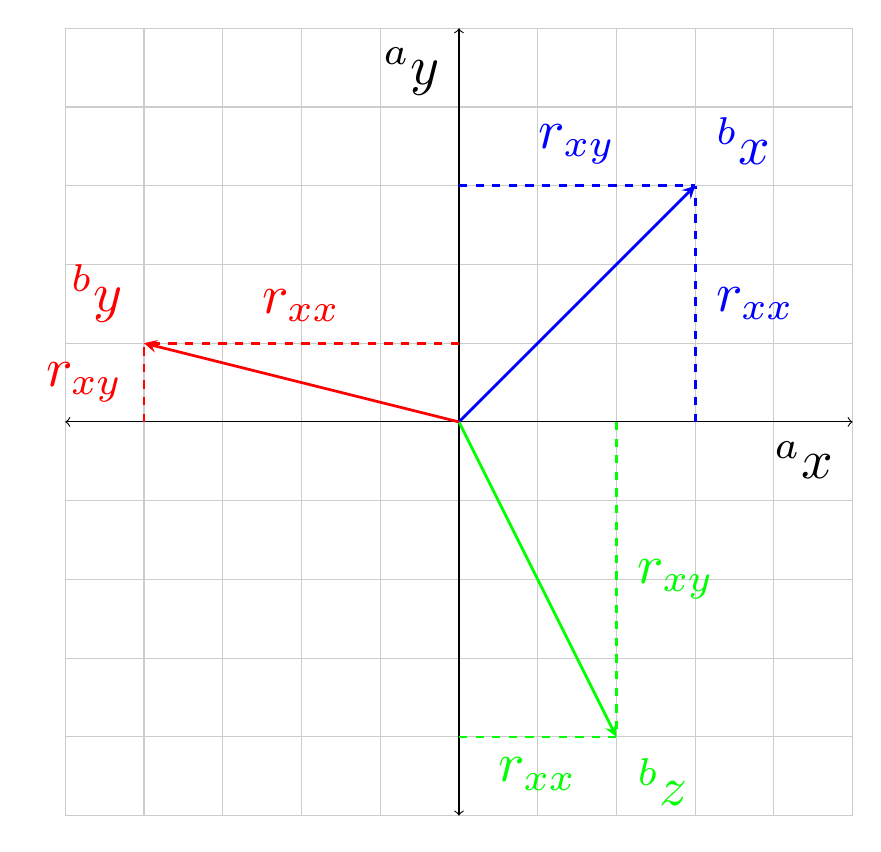
\begin{tikzpicture}
    \draw[thin,gray!40] (-5,-5) grid (5,5);
    \draw[<->] (-5,0)--(5,0) node[anchor=north east, scale=2]{$^{a}x$};
    \draw[<->] (0,-5)--(0,5) node[anchor=north east, scale=2]{$^{a}y$};
    \draw[line width=1pt,blue,-stealth](0,0)--(3,3) node[anchor=south west, scale=2]{$^{b}x$};
    \draw[line width=1pt,blue,dashed](3,0)--(3,3) node[midway, right, scale=2]{$r_{xx}$};
    \draw[line width=1pt,blue,dashed](0,3)--(3,3) node[midway, above, scale=2]{$r_{xy}$};
    \draw[line width=1pt,green,-stealth](0,0)--(2,-4) node[anchor=north west, scale=2]{${^{b}z}$};
    \draw[line width=1pt,green,dashed](0,-4)--(2,-4) node[midway, below, scale=2]{$r_{xx}$};
    \draw[line width=1pt,green,dashed](2,0)--(2,-4) node[midway, right, scale=2]{$r_{xy}$};
    \draw[line width=1pt,red,-stealth](0,0)--(-4,1) node[anchor=south east, scale=2]{${^{b}y}$};
    \draw[line width=1pt,red,dashed](0,1)--(-4,1) node[midway, above, scale=2]{$r_{xx}$};
    \draw[line width=1pt,red,dashed](-4,0)--(-4,1) node[midway, left, scale=2]{$r_{xy}$};
\end{tikzpicture}}
  \resizebox{0.54\linewidth}{!}{\tdplotsetmaincoords{40}{40}
\begin{tikzpicture}[tdplot_main_coords,font=\sffamily]
    \tdplotsetrotatedcoords{0}{0}{0}
    \begin{scope}[tdplot_rotated_coords]
        \begin{scope}[canvas is xy plane at z=0]
            \draw[thin,gray!40] (-5,-5) grid (5,5);
            % \fill[gray,fill opacity=0.3] (-2,-3) rectangle (2,3);
            \draw[-latex] (-5,0,0) -- (5,0,0)node[anchor=west]{$^{a}x$};
            \draw[-latex] (0,-5,0) -- (0,5,0)node[anchor=south]{$^{a}y$};
            \draw[line width=1pt,blue,dashed](3,0,0)--(3,3,0) node[midway, right, scale=2]{$r_{xy}$};
            \draw[line width=1pt,blue,dashed](0,3,0)--(3,3,0) node[midway, above, scale=2]{$r_{xx}$};
            \draw[line width=1pt,green,dashed](0,-4,0)--(2,-4,0) node[midway, below, scale=2]{$r_{zx}$};
            \draw[line width=1pt,green,dashed](2,0,0)--(2,-4,0) node[midway, right, scale=2]{$r_{zy}$};
            \draw[line width=1pt,red,dashed](0,1,0)--(-4,1,0) node[midway, above, scale=2]{$r_{yx}$};
            \draw[line width=1pt,red,dashed](-4,0,0)--(-4,1,0) node[midway, left, scale=2]{$r_{yy}$};
        \end{scope}
    \end{scope}
    \draw[line width=1pt,blue,-stealth](0,0,0)--(3,3,1) node[anchor=south west, scale=2]{$^{b}x$};
    \draw[line width=1pt,blue,dashed](3,3,0)--(3,3,1) node[midway, right, scale=2]{$r_{xz}$};
    \draw[line width=1pt,red,-stealth](0,0,0)--(-4,1,1) node[anchor=south east, scale=2]{${^{b}y}$};
    \draw[line width=1pt,red,dashed](-4,1,0)--(-4,1,1) node[midway, right, scale=2]{$r_{yz}$};
    \draw[line width=1pt,green,-stealth](0,0,0)--(2,-4,1) node[anchor=south east, scale=2]{${^{b}z}$};
    \draw[line width=1pt,green,dashed](2,-4,0)--(2,-4,1) node[midway, right, scale=2]{$r_{zz}$};
    \draw[-latex] (0,0,0) -- (0,0,6)node[anchor=north]{$^{a}z$};
\end{tikzpicture}}
  \caption{frame axis example.}
  \label{fig:axes_frames}
\end{figure}

In equation \ref{eq:rotation_matrices}, $R$ is a rotation matrix that can be applied to represent a composition of intrinsic rotations about axes $X$, $Y$, $Z$, (in that order), or a composition of extrinsic rotations about axes $Z$, $Y$, $X$ (in that order). The convention used in this work is represented by equation \ref{eq:axes_frames} and maps quantities described in frame $b$ to frame $a$. Comparing the structure of (2.3) with figure \ref{fig:axes_frames} it is seen that columns of $^a_bR$ represent each unity vector defining all axes of frame $b$.

\begin{equation}
  \textrm{$_{b}^{a}R$}
  =
  \begin{bmatrix}
    \textrm{$^{a}r_{xx}$} & \textrm{$^{a}r_{yx}$} & \textrm{$^{a}r_{zx}$} \\
    \textrm{$^{a}r_{xy}$} & \textrm{$^{a}r_{yy}$} & \textrm{$^{a}r_{zy}$} \\
    \textrm{$^{a}r_{xz}$} & \textrm{$^{a}r_{yz}$} & \textrm{$^{a}r_{zz}$} \\
  \end{bmatrix}
  \label{eq:axes_frames}
\end{equation}

Rotation matrices belong to the orthonormal group and one important property is that bRa bRT = I meaning a bRT = a bR-1 . Also a bRT is equal to b aR.

\subsubsection{Direct Cosine Matrix}

The direct cosine matrix (DCM) is similar to the rotational matrix, however it is a 3x3
matrix that contains the cosines of the 9 possible pairs of axes of two different Cartesian coordinate systems. The DCM is typically used to translate from the body frame into the earth frame. The DCM approach has gained much popularity for its advantage of
linear measurement equations in Kalman filters. \cite{premerlani2009direction}


\subsubsection{Euler angles}

Euler angles are a well-known form to represent attitude with respect to a fixed coordinate system. Mathematically, Euler angles represent three composed sequential rotations that stir a reference frame to a given referred frame \cite{diebel2006representing}. It expresses a rotation in three angles, often referred to as pitch, roll and yaw, denoted by $\phi$, $\theta$ and $\psi$ (The roll will have the range of $\pm180^\circ$, this allows the pitch to have the range of $\pm90^{\circ}$. The yaw is represented using the range of $\pm180^{\circ}$). These angles depict three successive rotations about the axes of the coordinate frame, for instance $x-y-z$: First rotate $\phi$ radians about the x-axis, then rotate $\theta$ radians about the y-axis and finally rotate $\psi$ radians about the z-axis \cite{grado1960solution}. As stated by the differential equations of Euler angles given at (equation \ref{eq:euler_equation}), $\phi$, $\theta$, and $\psi$ can be found based on angular rate measurements. Merely three differential equations require solving prior to the attitude gets distinctly approximated \cite{bar1985attitude}.

% \begin{figure}[!h]
%     \centering
%     \resizebox{0.70\linewidth}{!}{%% Creator: Matplotlib, PGF backend
%%
%% To include the figure in your LaTeX document, write
%%   \input{<filename>.pgf}
%%
%% Make sure the required packages are loaded in your preamble
%%   \usepackage{pgf}
%%
%% and, on pdftex
%%   \usepackage[utf8]{inputenc}\DeclareUnicodeCharacter{2212}{-}
%%
%% or, on luatex and xetex
%%   \usepackage{unicode-math}
%%
%% Figures using additional raster images can only be included by \input if
%% they are in the same directory as the main LaTeX file. For loading figures
%% from other directories you can use the `import` package
%%   \usepackage{import}
%%
%% and then include the figures with
%%   \import{<path to file>}{<filename>.pgf}
%%
%% Matplotlib used the following preamble
%%   \usepackage{fontspec}
%%
\begingroup%
\makeatletter%
\begin{pgfpicture}%
\pgfpathrectangle{\pgfpointorigin}{\pgfqpoint{6.400000in}{4.800000in}}%
\pgfusepath{use as bounding box, clip}%
\begin{pgfscope}%
\pgfsetbuttcap%
\pgfsetmiterjoin%
\definecolor{currentfill}{rgb}{1.000000,1.000000,1.000000}%
\pgfsetfillcolor{currentfill}%
\pgfsetlinewidth{0.000000pt}%
\definecolor{currentstroke}{rgb}{1.000000,1.000000,1.000000}%
\pgfsetstrokecolor{currentstroke}%
\pgfsetdash{}{0pt}%
\pgfpathmoveto{\pgfqpoint{0.000000in}{0.000000in}}%
\pgfpathlineto{\pgfqpoint{6.400000in}{0.000000in}}%
\pgfpathlineto{\pgfqpoint{6.400000in}{4.800000in}}%
\pgfpathlineto{\pgfqpoint{0.000000in}{4.800000in}}%
\pgfpathclose%
\pgfusepath{fill}%
\end{pgfscope}%
\begin{pgfscope}%
\pgfsetbuttcap%
\pgfsetmiterjoin%
\definecolor{currentfill}{rgb}{1.000000,1.000000,1.000000}%
\pgfsetfillcolor{currentfill}%
\pgfsetlinewidth{0.000000pt}%
\definecolor{currentstroke}{rgb}{0.000000,0.000000,0.000000}%
\pgfsetstrokecolor{currentstroke}%
\pgfsetstrokeopacity{0.000000}%
\pgfsetdash{}{0pt}%
\pgfpathmoveto{\pgfqpoint{0.758056in}{0.565000in}}%
\pgfpathlineto{\pgfqpoint{6.250000in}{0.565000in}}%
\pgfpathlineto{\pgfqpoint{6.250000in}{4.650000in}}%
\pgfpathlineto{\pgfqpoint{0.758056in}{4.650000in}}%
\pgfpathclose%
\pgfusepath{fill}%
\end{pgfscope}%
\begin{pgfscope}%
\pgfsetbuttcap%
\pgfsetroundjoin%
\definecolor{currentfill}{rgb}{0.000000,0.000000,0.000000}%
\pgfsetfillcolor{currentfill}%
\pgfsetlinewidth{0.803000pt}%
\definecolor{currentstroke}{rgb}{0.000000,0.000000,0.000000}%
\pgfsetstrokecolor{currentstroke}%
\pgfsetdash{}{0pt}%
\pgfsys@defobject{currentmarker}{\pgfqpoint{0.000000in}{-0.048611in}}{\pgfqpoint{0.000000in}{0.000000in}}{%
\pgfpathmoveto{\pgfqpoint{0.000000in}{0.000000in}}%
\pgfpathlineto{\pgfqpoint{0.000000in}{-0.048611in}}%
\pgfusepath{stroke,fill}%
}%
\begin{pgfscope}%
\pgfsys@transformshift{1.007690in}{0.565000in}%
\pgfsys@useobject{currentmarker}{}%
\end{pgfscope}%
\end{pgfscope}%
\begin{pgfscope}%
\definecolor{textcolor}{rgb}{0.000000,0.000000,0.000000}%
\pgfsetstrokecolor{textcolor}%
\pgfsetfillcolor{textcolor}%
\pgftext[x=1.007690in,y=0.467777in,,top]{\color{textcolor}\rmfamily\fontsize{10.000000}{12.000000}\selectfont \(\displaystyle {0}\)}%
\end{pgfscope}%
\begin{pgfscope}%
\pgfsetbuttcap%
\pgfsetroundjoin%
\definecolor{currentfill}{rgb}{0.000000,0.000000,0.000000}%
\pgfsetfillcolor{currentfill}%
\pgfsetlinewidth{0.803000pt}%
\definecolor{currentstroke}{rgb}{0.000000,0.000000,0.000000}%
\pgfsetstrokecolor{currentstroke}%
\pgfsetdash{}{0pt}%
\pgfsys@defobject{currentmarker}{\pgfqpoint{0.000000in}{-0.048611in}}{\pgfqpoint{0.000000in}{0.000000in}}{%
\pgfpathmoveto{\pgfqpoint{0.000000in}{0.000000in}}%
\pgfpathlineto{\pgfqpoint{0.000000in}{-0.048611in}}%
\pgfusepath{stroke,fill}%
}%
\begin{pgfscope}%
\pgfsys@transformshift{1.675160in}{0.565000in}%
\pgfsys@useobject{currentmarker}{}%
\end{pgfscope}%
\end{pgfscope}%
\begin{pgfscope}%
\definecolor{textcolor}{rgb}{0.000000,0.000000,0.000000}%
\pgfsetstrokecolor{textcolor}%
\pgfsetfillcolor{textcolor}%
\pgftext[x=1.675160in,y=0.467777in,,top]{\color{textcolor}\rmfamily\fontsize{10.000000}{12.000000}\selectfont \(\displaystyle {500}\)}%
\end{pgfscope}%
\begin{pgfscope}%
\pgfsetbuttcap%
\pgfsetroundjoin%
\definecolor{currentfill}{rgb}{0.000000,0.000000,0.000000}%
\pgfsetfillcolor{currentfill}%
\pgfsetlinewidth{0.803000pt}%
\definecolor{currentstroke}{rgb}{0.000000,0.000000,0.000000}%
\pgfsetstrokecolor{currentstroke}%
\pgfsetdash{}{0pt}%
\pgfsys@defobject{currentmarker}{\pgfqpoint{0.000000in}{-0.048611in}}{\pgfqpoint{0.000000in}{0.000000in}}{%
\pgfpathmoveto{\pgfqpoint{0.000000in}{0.000000in}}%
\pgfpathlineto{\pgfqpoint{0.000000in}{-0.048611in}}%
\pgfusepath{stroke,fill}%
}%
\begin{pgfscope}%
\pgfsys@transformshift{2.342630in}{0.565000in}%
\pgfsys@useobject{currentmarker}{}%
\end{pgfscope}%
\end{pgfscope}%
\begin{pgfscope}%
\definecolor{textcolor}{rgb}{0.000000,0.000000,0.000000}%
\pgfsetstrokecolor{textcolor}%
\pgfsetfillcolor{textcolor}%
\pgftext[x=2.342630in,y=0.467777in,,top]{\color{textcolor}\rmfamily\fontsize{10.000000}{12.000000}\selectfont \(\displaystyle {1000}\)}%
\end{pgfscope}%
\begin{pgfscope}%
\pgfsetbuttcap%
\pgfsetroundjoin%
\definecolor{currentfill}{rgb}{0.000000,0.000000,0.000000}%
\pgfsetfillcolor{currentfill}%
\pgfsetlinewidth{0.803000pt}%
\definecolor{currentstroke}{rgb}{0.000000,0.000000,0.000000}%
\pgfsetstrokecolor{currentstroke}%
\pgfsetdash{}{0pt}%
\pgfsys@defobject{currentmarker}{\pgfqpoint{0.000000in}{-0.048611in}}{\pgfqpoint{0.000000in}{0.000000in}}{%
\pgfpathmoveto{\pgfqpoint{0.000000in}{0.000000in}}%
\pgfpathlineto{\pgfqpoint{0.000000in}{-0.048611in}}%
\pgfusepath{stroke,fill}%
}%
\begin{pgfscope}%
\pgfsys@transformshift{3.010100in}{0.565000in}%
\pgfsys@useobject{currentmarker}{}%
\end{pgfscope}%
\end{pgfscope}%
\begin{pgfscope}%
\definecolor{textcolor}{rgb}{0.000000,0.000000,0.000000}%
\pgfsetstrokecolor{textcolor}%
\pgfsetfillcolor{textcolor}%
\pgftext[x=3.010100in,y=0.467777in,,top]{\color{textcolor}\rmfamily\fontsize{10.000000}{12.000000}\selectfont \(\displaystyle {1500}\)}%
\end{pgfscope}%
\begin{pgfscope}%
\pgfsetbuttcap%
\pgfsetroundjoin%
\definecolor{currentfill}{rgb}{0.000000,0.000000,0.000000}%
\pgfsetfillcolor{currentfill}%
\pgfsetlinewidth{0.803000pt}%
\definecolor{currentstroke}{rgb}{0.000000,0.000000,0.000000}%
\pgfsetstrokecolor{currentstroke}%
\pgfsetdash{}{0pt}%
\pgfsys@defobject{currentmarker}{\pgfqpoint{0.000000in}{-0.048611in}}{\pgfqpoint{0.000000in}{0.000000in}}{%
\pgfpathmoveto{\pgfqpoint{0.000000in}{0.000000in}}%
\pgfpathlineto{\pgfqpoint{0.000000in}{-0.048611in}}%
\pgfusepath{stroke,fill}%
}%
\begin{pgfscope}%
\pgfsys@transformshift{3.677570in}{0.565000in}%
\pgfsys@useobject{currentmarker}{}%
\end{pgfscope}%
\end{pgfscope}%
\begin{pgfscope}%
\definecolor{textcolor}{rgb}{0.000000,0.000000,0.000000}%
\pgfsetstrokecolor{textcolor}%
\pgfsetfillcolor{textcolor}%
\pgftext[x=3.677570in,y=0.467777in,,top]{\color{textcolor}\rmfamily\fontsize{10.000000}{12.000000}\selectfont \(\displaystyle {2000}\)}%
\end{pgfscope}%
\begin{pgfscope}%
\pgfsetbuttcap%
\pgfsetroundjoin%
\definecolor{currentfill}{rgb}{0.000000,0.000000,0.000000}%
\pgfsetfillcolor{currentfill}%
\pgfsetlinewidth{0.803000pt}%
\definecolor{currentstroke}{rgb}{0.000000,0.000000,0.000000}%
\pgfsetstrokecolor{currentstroke}%
\pgfsetdash{}{0pt}%
\pgfsys@defobject{currentmarker}{\pgfqpoint{0.000000in}{-0.048611in}}{\pgfqpoint{0.000000in}{0.000000in}}{%
\pgfpathmoveto{\pgfqpoint{0.000000in}{0.000000in}}%
\pgfpathlineto{\pgfqpoint{0.000000in}{-0.048611in}}%
\pgfusepath{stroke,fill}%
}%
\begin{pgfscope}%
\pgfsys@transformshift{4.345040in}{0.565000in}%
\pgfsys@useobject{currentmarker}{}%
\end{pgfscope}%
\end{pgfscope}%
\begin{pgfscope}%
\definecolor{textcolor}{rgb}{0.000000,0.000000,0.000000}%
\pgfsetstrokecolor{textcolor}%
\pgfsetfillcolor{textcolor}%
\pgftext[x=4.345040in,y=0.467777in,,top]{\color{textcolor}\rmfamily\fontsize{10.000000}{12.000000}\selectfont \(\displaystyle {2500}\)}%
\end{pgfscope}%
\begin{pgfscope}%
\pgfsetbuttcap%
\pgfsetroundjoin%
\definecolor{currentfill}{rgb}{0.000000,0.000000,0.000000}%
\pgfsetfillcolor{currentfill}%
\pgfsetlinewidth{0.803000pt}%
\definecolor{currentstroke}{rgb}{0.000000,0.000000,0.000000}%
\pgfsetstrokecolor{currentstroke}%
\pgfsetdash{}{0pt}%
\pgfsys@defobject{currentmarker}{\pgfqpoint{0.000000in}{-0.048611in}}{\pgfqpoint{0.000000in}{0.000000in}}{%
\pgfpathmoveto{\pgfqpoint{0.000000in}{0.000000in}}%
\pgfpathlineto{\pgfqpoint{0.000000in}{-0.048611in}}%
\pgfusepath{stroke,fill}%
}%
\begin{pgfscope}%
\pgfsys@transformshift{5.012510in}{0.565000in}%
\pgfsys@useobject{currentmarker}{}%
\end{pgfscope}%
\end{pgfscope}%
\begin{pgfscope}%
\definecolor{textcolor}{rgb}{0.000000,0.000000,0.000000}%
\pgfsetstrokecolor{textcolor}%
\pgfsetfillcolor{textcolor}%
\pgftext[x=5.012510in,y=0.467777in,,top]{\color{textcolor}\rmfamily\fontsize{10.000000}{12.000000}\selectfont \(\displaystyle {3000}\)}%
\end{pgfscope}%
\begin{pgfscope}%
\pgfsetbuttcap%
\pgfsetroundjoin%
\definecolor{currentfill}{rgb}{0.000000,0.000000,0.000000}%
\pgfsetfillcolor{currentfill}%
\pgfsetlinewidth{0.803000pt}%
\definecolor{currentstroke}{rgb}{0.000000,0.000000,0.000000}%
\pgfsetstrokecolor{currentstroke}%
\pgfsetdash{}{0pt}%
\pgfsys@defobject{currentmarker}{\pgfqpoint{0.000000in}{-0.048611in}}{\pgfqpoint{0.000000in}{0.000000in}}{%
\pgfpathmoveto{\pgfqpoint{0.000000in}{0.000000in}}%
\pgfpathlineto{\pgfqpoint{0.000000in}{-0.048611in}}%
\pgfusepath{stroke,fill}%
}%
\begin{pgfscope}%
\pgfsys@transformshift{5.679981in}{0.565000in}%
\pgfsys@useobject{currentmarker}{}%
\end{pgfscope}%
\end{pgfscope}%
\begin{pgfscope}%
\definecolor{textcolor}{rgb}{0.000000,0.000000,0.000000}%
\pgfsetstrokecolor{textcolor}%
\pgfsetfillcolor{textcolor}%
\pgftext[x=5.679981in,y=0.467777in,,top]{\color{textcolor}\rmfamily\fontsize{10.000000}{12.000000}\selectfont \(\displaystyle {3500}\)}%
\end{pgfscope}%
\begin{pgfscope}%
\definecolor{textcolor}{rgb}{0.000000,0.000000,0.000000}%
\pgfsetstrokecolor{textcolor}%
\pgfsetfillcolor{textcolor}%
\pgftext[x=3.504028in,y=0.288889in,,top]{\color{textcolor}\rmfamily\fontsize{10.000000}{12.000000}\selectfont Samples [\#]}%
\end{pgfscope}%
\begin{pgfscope}%
\pgfsetbuttcap%
\pgfsetroundjoin%
\definecolor{currentfill}{rgb}{0.000000,0.000000,0.000000}%
\pgfsetfillcolor{currentfill}%
\pgfsetlinewidth{0.803000pt}%
\definecolor{currentstroke}{rgb}{0.000000,0.000000,0.000000}%
\pgfsetstrokecolor{currentstroke}%
\pgfsetdash{}{0pt}%
\pgfsys@defobject{currentmarker}{\pgfqpoint{-0.048611in}{0.000000in}}{\pgfqpoint{-0.000000in}{0.000000in}}{%
\pgfpathmoveto{\pgfqpoint{-0.000000in}{0.000000in}}%
\pgfpathlineto{\pgfqpoint{-0.048611in}{0.000000in}}%
\pgfusepath{stroke,fill}%
}%
\begin{pgfscope}%
\pgfsys@transformshift{0.758056in}{1.060029in}%
\pgfsys@useobject{currentmarker}{}%
\end{pgfscope}%
\end{pgfscope}%
\begin{pgfscope}%
\definecolor{textcolor}{rgb}{0.000000,0.000000,0.000000}%
\pgfsetstrokecolor{textcolor}%
\pgfsetfillcolor{textcolor}%
\pgftext[x=0.344444in, y=1.011834in, left, base]{\color{textcolor}\rmfamily\fontsize{10.000000}{12.000000}\selectfont \(\displaystyle {−150}\)}%
\end{pgfscope}%
\begin{pgfscope}%
\pgfsetbuttcap%
\pgfsetroundjoin%
\definecolor{currentfill}{rgb}{0.000000,0.000000,0.000000}%
\pgfsetfillcolor{currentfill}%
\pgfsetlinewidth{0.803000pt}%
\definecolor{currentstroke}{rgb}{0.000000,0.000000,0.000000}%
\pgfsetstrokecolor{currentstroke}%
\pgfsetdash{}{0pt}%
\pgfsys@defobject{currentmarker}{\pgfqpoint{-0.048611in}{0.000000in}}{\pgfqpoint{-0.000000in}{0.000000in}}{%
\pgfpathmoveto{\pgfqpoint{-0.000000in}{0.000000in}}%
\pgfpathlineto{\pgfqpoint{-0.048611in}{0.000000in}}%
\pgfusepath{stroke,fill}%
}%
\begin{pgfscope}%
\pgfsys@transformshift{0.758056in}{1.575861in}%
\pgfsys@useobject{currentmarker}{}%
\end{pgfscope}%
\end{pgfscope}%
\begin{pgfscope}%
\definecolor{textcolor}{rgb}{0.000000,0.000000,0.000000}%
\pgfsetstrokecolor{textcolor}%
\pgfsetfillcolor{textcolor}%
\pgftext[x=0.344444in, y=1.527666in, left, base]{\color{textcolor}\rmfamily\fontsize{10.000000}{12.000000}\selectfont \(\displaystyle {−100}\)}%
\end{pgfscope}%
\begin{pgfscope}%
\pgfsetbuttcap%
\pgfsetroundjoin%
\definecolor{currentfill}{rgb}{0.000000,0.000000,0.000000}%
\pgfsetfillcolor{currentfill}%
\pgfsetlinewidth{0.803000pt}%
\definecolor{currentstroke}{rgb}{0.000000,0.000000,0.000000}%
\pgfsetstrokecolor{currentstroke}%
\pgfsetdash{}{0pt}%
\pgfsys@defobject{currentmarker}{\pgfqpoint{-0.048611in}{0.000000in}}{\pgfqpoint{-0.000000in}{0.000000in}}{%
\pgfpathmoveto{\pgfqpoint{-0.000000in}{0.000000in}}%
\pgfpathlineto{\pgfqpoint{-0.048611in}{0.000000in}}%
\pgfusepath{stroke,fill}%
}%
\begin{pgfscope}%
\pgfsys@transformshift{0.758056in}{2.091693in}%
\pgfsys@useobject{currentmarker}{}%
\end{pgfscope}%
\end{pgfscope}%
\begin{pgfscope}%
\definecolor{textcolor}{rgb}{0.000000,0.000000,0.000000}%
\pgfsetstrokecolor{textcolor}%
\pgfsetfillcolor{textcolor}%
\pgftext[x=0.413889in, y=2.043499in, left, base]{\color{textcolor}\rmfamily\fontsize{10.000000}{12.000000}\selectfont \(\displaystyle {−50}\)}%
\end{pgfscope}%
\begin{pgfscope}%
\pgfsetbuttcap%
\pgfsetroundjoin%
\definecolor{currentfill}{rgb}{0.000000,0.000000,0.000000}%
\pgfsetfillcolor{currentfill}%
\pgfsetlinewidth{0.803000pt}%
\definecolor{currentstroke}{rgb}{0.000000,0.000000,0.000000}%
\pgfsetstrokecolor{currentstroke}%
\pgfsetdash{}{0pt}%
\pgfsys@defobject{currentmarker}{\pgfqpoint{-0.048611in}{0.000000in}}{\pgfqpoint{-0.000000in}{0.000000in}}{%
\pgfpathmoveto{\pgfqpoint{-0.000000in}{0.000000in}}%
\pgfpathlineto{\pgfqpoint{-0.048611in}{0.000000in}}%
\pgfusepath{stroke,fill}%
}%
\begin{pgfscope}%
\pgfsys@transformshift{0.758056in}{2.607525in}%
\pgfsys@useobject{currentmarker}{}%
\end{pgfscope}%
\end{pgfscope}%
\begin{pgfscope}%
\definecolor{textcolor}{rgb}{0.000000,0.000000,0.000000}%
\pgfsetstrokecolor{textcolor}%
\pgfsetfillcolor{textcolor}%
\pgftext[x=0.591389in, y=2.559331in, left, base]{\color{textcolor}\rmfamily\fontsize{10.000000}{12.000000}\selectfont \(\displaystyle {0}\)}%
\end{pgfscope}%
\begin{pgfscope}%
\pgfsetbuttcap%
\pgfsetroundjoin%
\definecolor{currentfill}{rgb}{0.000000,0.000000,0.000000}%
\pgfsetfillcolor{currentfill}%
\pgfsetlinewidth{0.803000pt}%
\definecolor{currentstroke}{rgb}{0.000000,0.000000,0.000000}%
\pgfsetstrokecolor{currentstroke}%
\pgfsetdash{}{0pt}%
\pgfsys@defobject{currentmarker}{\pgfqpoint{-0.048611in}{0.000000in}}{\pgfqpoint{-0.000000in}{0.000000in}}{%
\pgfpathmoveto{\pgfqpoint{-0.000000in}{0.000000in}}%
\pgfpathlineto{\pgfqpoint{-0.048611in}{0.000000in}}%
\pgfusepath{stroke,fill}%
}%
\begin{pgfscope}%
\pgfsys@transformshift{0.758056in}{3.123357in}%
\pgfsys@useobject{currentmarker}{}%
\end{pgfscope}%
\end{pgfscope}%
\begin{pgfscope}%
\definecolor{textcolor}{rgb}{0.000000,0.000000,0.000000}%
\pgfsetstrokecolor{textcolor}%
\pgfsetfillcolor{textcolor}%
\pgftext[x=0.521944in, y=3.075163in, left, base]{\color{textcolor}\rmfamily\fontsize{10.000000}{12.000000}\selectfont \(\displaystyle {50}\)}%
\end{pgfscope}%
\begin{pgfscope}%
\pgfsetbuttcap%
\pgfsetroundjoin%
\definecolor{currentfill}{rgb}{0.000000,0.000000,0.000000}%
\pgfsetfillcolor{currentfill}%
\pgfsetlinewidth{0.803000pt}%
\definecolor{currentstroke}{rgb}{0.000000,0.000000,0.000000}%
\pgfsetstrokecolor{currentstroke}%
\pgfsetdash{}{0pt}%
\pgfsys@defobject{currentmarker}{\pgfqpoint{-0.048611in}{0.000000in}}{\pgfqpoint{-0.000000in}{0.000000in}}{%
\pgfpathmoveto{\pgfqpoint{-0.000000in}{0.000000in}}%
\pgfpathlineto{\pgfqpoint{-0.048611in}{0.000000in}}%
\pgfusepath{stroke,fill}%
}%
\begin{pgfscope}%
\pgfsys@transformshift{0.758056in}{3.639190in}%
\pgfsys@useobject{currentmarker}{}%
\end{pgfscope}%
\end{pgfscope}%
\begin{pgfscope}%
\definecolor{textcolor}{rgb}{0.000000,0.000000,0.000000}%
\pgfsetstrokecolor{textcolor}%
\pgfsetfillcolor{textcolor}%
\pgftext[x=0.452500in, y=3.590995in, left, base]{\color{textcolor}\rmfamily\fontsize{10.000000}{12.000000}\selectfont \(\displaystyle {100}\)}%
\end{pgfscope}%
\begin{pgfscope}%
\pgfsetbuttcap%
\pgfsetroundjoin%
\definecolor{currentfill}{rgb}{0.000000,0.000000,0.000000}%
\pgfsetfillcolor{currentfill}%
\pgfsetlinewidth{0.803000pt}%
\definecolor{currentstroke}{rgb}{0.000000,0.000000,0.000000}%
\pgfsetstrokecolor{currentstroke}%
\pgfsetdash{}{0pt}%
\pgfsys@defobject{currentmarker}{\pgfqpoint{-0.048611in}{0.000000in}}{\pgfqpoint{-0.000000in}{0.000000in}}{%
\pgfpathmoveto{\pgfqpoint{-0.000000in}{0.000000in}}%
\pgfpathlineto{\pgfqpoint{-0.048611in}{0.000000in}}%
\pgfusepath{stroke,fill}%
}%
\begin{pgfscope}%
\pgfsys@transformshift{0.758056in}{4.155022in}%
\pgfsys@useobject{currentmarker}{}%
\end{pgfscope}%
\end{pgfscope}%
\begin{pgfscope}%
\definecolor{textcolor}{rgb}{0.000000,0.000000,0.000000}%
\pgfsetstrokecolor{textcolor}%
\pgfsetfillcolor{textcolor}%
\pgftext[x=0.452500in, y=4.106827in, left, base]{\color{textcolor}\rmfamily\fontsize{10.000000}{12.000000}\selectfont \(\displaystyle {150}\)}%
\end{pgfscope}%
\begin{pgfscope}%
\definecolor{textcolor}{rgb}{0.000000,0.000000,0.000000}%
\pgfsetstrokecolor{textcolor}%
\pgfsetfillcolor{textcolor}%
\pgftext[x=0.288889in,y=2.607500in,,bottom,rotate=90.000000]{\color{textcolor}\rmfamily\fontsize{10.000000}{12.000000}\selectfont Degrees [\(\displaystyle \circ\)]}%
\end{pgfscope}%
\begin{pgfscope}%
\pgfpathrectangle{\pgfqpoint{0.758056in}{0.565000in}}{\pgfqpoint{5.491944in}{4.085000in}}%
\pgfusepath{clip}%
\pgfsetrectcap%
\pgfsetroundjoin%
\pgfsetlinewidth{1.505625pt}%
\definecolor{currentstroke}{rgb}{0.121569,0.466667,0.705882}%
\pgfsetstrokecolor{currentstroke}%
\pgfsetdash{}{0pt}%
\pgfpathmoveto{\pgfqpoint{1.007690in}{2.724542in}}%
\pgfpathlineto{\pgfqpoint{1.071767in}{2.675383in}}%
\pgfpathlineto{\pgfqpoint{1.079776in}{2.670549in}}%
\pgfpathlineto{\pgfqpoint{1.081111in}{2.671453in}}%
\pgfpathlineto{\pgfqpoint{1.083781in}{2.678801in}}%
\pgfpathlineto{\pgfqpoint{1.086451in}{2.682270in}}%
\pgfpathlineto{\pgfqpoint{1.098466in}{2.693299in}}%
\pgfpathlineto{\pgfqpoint{1.115820in}{2.716741in}}%
\pgfpathlineto{\pgfqpoint{1.157203in}{2.773058in}}%
\pgfpathlineto{\pgfqpoint{1.167882in}{2.785655in}}%
\pgfpathlineto{\pgfqpoint{1.187907in}{2.805131in}}%
\pgfpathlineto{\pgfqpoint{1.203926in}{2.816865in}}%
\pgfpathlineto{\pgfqpoint{1.215940in}{2.822464in}}%
\pgfpathlineto{\pgfqpoint{1.226620in}{2.824642in}}%
\pgfpathlineto{\pgfqpoint{1.239969in}{2.824348in}}%
\pgfpathlineto{\pgfqpoint{1.250649in}{2.821668in}}%
\pgfpathlineto{\pgfqpoint{1.255989in}{2.819075in}}%
\pgfpathlineto{\pgfqpoint{1.268003in}{2.813168in}}%
\pgfpathlineto{\pgfqpoint{1.270673in}{2.815306in}}%
\pgfpathlineto{\pgfqpoint{1.273343in}{2.812502in}}%
\pgfpathlineto{\pgfqpoint{1.276013in}{2.810772in}}%
\pgfpathlineto{\pgfqpoint{1.277348in}{2.811208in}}%
\pgfpathlineto{\pgfqpoint{1.280017in}{2.808179in}}%
\pgfpathlineto{\pgfqpoint{1.282687in}{2.808013in}}%
\pgfpathlineto{\pgfqpoint{1.286692in}{2.808331in}}%
\pgfpathlineto{\pgfqpoint{1.294702in}{2.806901in}}%
\pgfpathlineto{\pgfqpoint{1.308051in}{2.801757in}}%
\pgfpathlineto{\pgfqpoint{1.310721in}{2.800398in}}%
\pgfpathlineto{\pgfqpoint{1.312056in}{2.800785in}}%
\pgfpathlineto{\pgfqpoint{1.314726in}{2.798967in}}%
\pgfpathlineto{\pgfqpoint{1.317396in}{2.798193in}}%
\pgfpathlineto{\pgfqpoint{1.324070in}{2.798450in}}%
\pgfpathlineto{\pgfqpoint{1.325405in}{2.796735in}}%
\pgfpathlineto{\pgfqpoint{1.326740in}{2.797304in}}%
\pgfpathlineto{\pgfqpoint{1.332080in}{2.792921in}}%
\pgfpathlineto{\pgfqpoint{1.336085in}{2.793024in}}%
\pgfpathlineto{\pgfqpoint{1.337420in}{2.794142in}}%
\pgfpathlineto{\pgfqpoint{1.338755in}{2.793663in}}%
\pgfpathlineto{\pgfqpoint{1.341425in}{2.794128in}}%
\pgfpathlineto{\pgfqpoint{1.342760in}{2.793698in}}%
\pgfpathlineto{\pgfqpoint{1.344095in}{2.791982in}}%
\pgfpathlineto{\pgfqpoint{1.345430in}{2.792622in}}%
\pgfpathlineto{\pgfqpoint{1.349434in}{2.789025in}}%
\pgfpathlineto{\pgfqpoint{1.350769in}{2.787611in}}%
\pgfpathlineto{\pgfqpoint{1.352104in}{2.789122in}}%
\pgfpathlineto{\pgfqpoint{1.356109in}{2.786256in}}%
\pgfpathlineto{\pgfqpoint{1.360114in}{2.785592in}}%
\pgfpathlineto{\pgfqpoint{1.361449in}{2.786379in}}%
\pgfpathlineto{\pgfqpoint{1.362784in}{2.784345in}}%
\pgfpathlineto{\pgfqpoint{1.364119in}{2.780091in}}%
\pgfpathlineto{\pgfqpoint{1.365454in}{2.781644in}}%
\pgfpathlineto{\pgfqpoint{1.366789in}{2.780266in}}%
\pgfpathlineto{\pgfqpoint{1.373463in}{2.781638in}}%
\pgfpathlineto{\pgfqpoint{1.377468in}{2.777666in}}%
\pgfpathlineto{\pgfqpoint{1.386813in}{2.770906in}}%
\pgfpathlineto{\pgfqpoint{1.389483in}{2.770978in}}%
\pgfpathlineto{\pgfqpoint{1.393487in}{2.764674in}}%
\pgfpathlineto{\pgfqpoint{1.410842in}{2.730634in}}%
\pgfpathlineto{\pgfqpoint{1.416181in}{2.721050in}}%
\pgfpathlineto{\pgfqpoint{1.434871in}{2.681440in}}%
\pgfpathlineto{\pgfqpoint{1.446885in}{2.655493in}}%
\pgfpathlineto{\pgfqpoint{1.454895in}{2.637857in}}%
\pgfpathlineto{\pgfqpoint{1.461569in}{2.623457in}}%
\pgfpathlineto{\pgfqpoint{1.468244in}{2.609843in}}%
\pgfpathlineto{\pgfqpoint{1.477589in}{2.589391in}}%
\pgfpathlineto{\pgfqpoint{1.500283in}{2.540512in}}%
\pgfpathlineto{\pgfqpoint{1.506957in}{2.526043in}}%
\pgfpathlineto{\pgfqpoint{1.532321in}{2.478892in}}%
\pgfpathlineto{\pgfqpoint{1.544336in}{2.455129in}}%
\pgfpathlineto{\pgfqpoint{1.551010in}{2.440628in}}%
\pgfpathlineto{\pgfqpoint{1.583049in}{2.359317in}}%
\pgfpathlineto{\pgfqpoint{1.589724in}{2.340371in}}%
\pgfpathlineto{\pgfqpoint{1.615087in}{2.279915in}}%
\pgfpathlineto{\pgfqpoint{1.617757in}{2.275624in}}%
\pgfpathlineto{\pgfqpoint{1.621762in}{2.267553in}}%
\pgfpathlineto{\pgfqpoint{1.627102in}{2.263423in}}%
\pgfpathlineto{\pgfqpoint{1.629772in}{2.262033in}}%
\pgfpathlineto{\pgfqpoint{1.635112in}{2.255932in}}%
\pgfpathlineto{\pgfqpoint{1.636447in}{2.255420in}}%
\pgfpathlineto{\pgfqpoint{1.639116in}{2.252718in}}%
\pgfpathlineto{\pgfqpoint{1.648461in}{2.248026in}}%
\pgfpathlineto{\pgfqpoint{1.651131in}{2.246601in}}%
\pgfpathlineto{\pgfqpoint{1.652466in}{2.247039in}}%
\pgfpathlineto{\pgfqpoint{1.655136in}{2.244179in}}%
\pgfpathlineto{\pgfqpoint{1.657806in}{2.242876in}}%
\pgfpathlineto{\pgfqpoint{1.659140in}{2.243675in}}%
\pgfpathlineto{\pgfqpoint{1.661810in}{2.243340in}}%
\pgfpathlineto{\pgfqpoint{1.665815in}{2.244148in}}%
\pgfpathlineto{\pgfqpoint{1.668485in}{2.246193in}}%
\pgfpathlineto{\pgfqpoint{1.671155in}{2.245549in}}%
\pgfpathlineto{\pgfqpoint{1.673825in}{2.247226in}}%
\pgfpathlineto{\pgfqpoint{1.677830in}{2.247180in}}%
\pgfpathlineto{\pgfqpoint{1.679165in}{2.248255in}}%
\pgfpathlineto{\pgfqpoint{1.681834in}{2.246288in}}%
\pgfpathlineto{\pgfqpoint{1.687174in}{2.249029in}}%
\pgfpathlineto{\pgfqpoint{1.689844in}{2.248375in}}%
\pgfpathlineto{\pgfqpoint{1.691179in}{2.250298in}}%
\pgfpathlineto{\pgfqpoint{1.692514in}{2.248917in}}%
\pgfpathlineto{\pgfqpoint{1.693849in}{2.250298in}}%
\pgfpathlineto{\pgfqpoint{1.699189in}{2.248698in}}%
\pgfpathlineto{\pgfqpoint{1.701859in}{2.249661in}}%
\pgfpathlineto{\pgfqpoint{1.704528in}{2.247502in}}%
\pgfpathlineto{\pgfqpoint{1.705863in}{2.248073in}}%
\pgfpathlineto{\pgfqpoint{1.707198in}{2.247025in}}%
\pgfpathlineto{\pgfqpoint{1.709868in}{2.248165in}}%
\pgfpathlineto{\pgfqpoint{1.715208in}{2.243571in}}%
\pgfpathlineto{\pgfqpoint{1.716543in}{2.244272in}}%
\pgfpathlineto{\pgfqpoint{1.719213in}{2.249952in}}%
\pgfpathlineto{\pgfqpoint{1.735232in}{2.291262in}}%
\pgfpathlineto{\pgfqpoint{1.743242in}{2.307640in}}%
\pgfpathlineto{\pgfqpoint{1.755256in}{2.331011in}}%
\pgfpathlineto{\pgfqpoint{1.765936in}{2.349058in}}%
\pgfpathlineto{\pgfqpoint{1.769941in}{2.356123in}}%
\pgfpathlineto{\pgfqpoint{1.793969in}{2.402981in}}%
\pgfpathlineto{\pgfqpoint{1.801979in}{2.421528in}}%
\pgfpathlineto{\pgfqpoint{1.808654in}{2.440993in}}%
\pgfpathlineto{\pgfqpoint{1.809989in}{2.441332in}}%
\pgfpathlineto{\pgfqpoint{1.813994in}{2.445663in}}%
\pgfpathlineto{\pgfqpoint{1.820668in}{2.452619in}}%
\pgfpathlineto{\pgfqpoint{1.830013in}{2.464242in}}%
\pgfpathlineto{\pgfqpoint{1.912779in}{2.583661in}}%
\pgfpathlineto{\pgfqpoint{1.914114in}{2.584032in}}%
\pgfpathlineto{\pgfqpoint{1.915449in}{2.582973in}}%
\pgfpathlineto{\pgfqpoint{1.916784in}{2.583574in}}%
\pgfpathlineto{\pgfqpoint{1.926129in}{2.577950in}}%
\pgfpathlineto{\pgfqpoint{1.932803in}{2.574383in}}%
\pgfpathlineto{\pgfqpoint{1.936808in}{2.572060in}}%
\pgfpathlineto{\pgfqpoint{1.943483in}{2.567784in}}%
\pgfpathlineto{\pgfqpoint{1.946153in}{2.565463in}}%
\pgfpathlineto{\pgfqpoint{1.954162in}{2.561391in}}%
\pgfpathlineto{\pgfqpoint{1.956832in}{2.559099in}}%
\pgfpathlineto{\pgfqpoint{1.958167in}{2.559803in}}%
\pgfpathlineto{\pgfqpoint{1.960837in}{2.557223in}}%
\pgfpathlineto{\pgfqpoint{1.963507in}{2.555782in}}%
\pgfpathlineto{\pgfqpoint{1.966177in}{2.554268in}}%
\pgfpathlineto{\pgfqpoint{1.968847in}{2.551706in}}%
\pgfpathlineto{\pgfqpoint{1.971517in}{2.550714in}}%
\pgfpathlineto{\pgfqpoint{1.974186in}{2.548164in}}%
\pgfpathlineto{\pgfqpoint{1.976856in}{2.547991in}}%
\pgfpathlineto{\pgfqpoint{1.980861in}{2.545217in}}%
\pgfpathlineto{\pgfqpoint{1.983531in}{2.543699in}}%
\pgfpathlineto{\pgfqpoint{1.991541in}{2.538375in}}%
\pgfpathlineto{\pgfqpoint{1.994210in}{2.538370in}}%
\pgfpathlineto{\pgfqpoint{1.998215in}{2.535262in}}%
\pgfpathlineto{\pgfqpoint{1.999550in}{2.535628in}}%
\pgfpathlineto{\pgfqpoint{2.004890in}{2.530767in}}%
\pgfpathlineto{\pgfqpoint{2.006225in}{2.531481in}}%
\pgfpathlineto{\pgfqpoint{2.008895in}{2.529099in}}%
\pgfpathlineto{\pgfqpoint{2.011565in}{2.527307in}}%
\pgfpathlineto{\pgfqpoint{2.012900in}{2.527798in}}%
\pgfpathlineto{\pgfqpoint{2.028919in}{2.512902in}}%
\pgfpathlineto{\pgfqpoint{2.031589in}{2.509318in}}%
\pgfpathlineto{\pgfqpoint{2.034259in}{2.510476in}}%
\pgfpathlineto{\pgfqpoint{2.039598in}{2.507513in}}%
\pgfpathlineto{\pgfqpoint{2.040933in}{2.508175in}}%
\pgfpathlineto{\pgfqpoint{2.046273in}{2.503176in}}%
\pgfpathlineto{\pgfqpoint{2.047608in}{2.504824in}}%
\pgfpathlineto{\pgfqpoint{2.051613in}{2.501396in}}%
\pgfpathlineto{\pgfqpoint{2.058288in}{2.494264in}}%
\pgfpathlineto{\pgfqpoint{2.062292in}{2.488028in}}%
\pgfpathlineto{\pgfqpoint{2.064962in}{2.485236in}}%
\pgfpathlineto{\pgfqpoint{2.074307in}{2.469611in}}%
\pgfpathlineto{\pgfqpoint{2.087656in}{2.435817in}}%
\pgfpathlineto{\pgfqpoint{2.094331in}{2.417873in}}%
\pgfpathlineto{\pgfqpoint{2.101006in}{2.401564in}}%
\pgfpathlineto{\pgfqpoint{2.109015in}{2.380847in}}%
\pgfpathlineto{\pgfqpoint{2.113020in}{2.369449in}}%
\pgfpathlineto{\pgfqpoint{2.115690in}{2.362262in}}%
\pgfpathlineto{\pgfqpoint{2.122365in}{2.341677in}}%
\pgfpathlineto{\pgfqpoint{2.137049in}{2.301822in}}%
\pgfpathlineto{\pgfqpoint{2.151733in}{2.265445in}}%
\pgfpathlineto{\pgfqpoint{2.161078in}{2.249445in}}%
\pgfpathlineto{\pgfqpoint{2.165083in}{2.244052in}}%
\pgfpathlineto{\pgfqpoint{2.169088in}{2.239360in}}%
\pgfpathlineto{\pgfqpoint{2.171758in}{2.236894in}}%
\pgfpathlineto{\pgfqpoint{2.182437in}{2.225617in}}%
\pgfpathlineto{\pgfqpoint{2.186442in}{2.224189in}}%
\pgfpathlineto{\pgfqpoint{2.187777in}{2.223444in}}%
\pgfpathlineto{\pgfqpoint{2.189112in}{2.224563in}}%
\pgfpathlineto{\pgfqpoint{2.191782in}{2.221759in}}%
\pgfpathlineto{\pgfqpoint{2.194452in}{2.219659in}}%
\pgfpathlineto{\pgfqpoint{2.195786in}{2.220362in}}%
\pgfpathlineto{\pgfqpoint{2.201126in}{2.217216in}}%
\pgfpathlineto{\pgfqpoint{2.203796in}{2.216557in}}%
\pgfpathlineto{\pgfqpoint{2.205131in}{2.214382in}}%
\pgfpathlineto{\pgfqpoint{2.206466in}{2.216177in}}%
\pgfpathlineto{\pgfqpoint{2.209136in}{2.215696in}}%
\pgfpathlineto{\pgfqpoint{2.213141in}{2.217832in}}%
\pgfpathlineto{\pgfqpoint{2.221150in}{2.216398in}}%
\pgfpathlineto{\pgfqpoint{2.223820in}{2.218220in}}%
\pgfpathlineto{\pgfqpoint{2.227825in}{2.215622in}}%
\pgfpathlineto{\pgfqpoint{2.230495in}{2.217628in}}%
\pgfpathlineto{\pgfqpoint{2.233165in}{2.215711in}}%
\pgfpathlineto{\pgfqpoint{2.234500in}{2.216256in}}%
\pgfpathlineto{\pgfqpoint{2.235835in}{2.218836in}}%
\pgfpathlineto{\pgfqpoint{2.239840in}{2.218772in}}%
\pgfpathlineto{\pgfqpoint{2.245179in}{2.223344in}}%
\pgfpathlineto{\pgfqpoint{2.251854in}{2.219583in}}%
\pgfpathlineto{\pgfqpoint{2.254524in}{2.220350in}}%
\pgfpathlineto{\pgfqpoint{2.255859in}{2.218913in}}%
\pgfpathlineto{\pgfqpoint{2.257194in}{2.220247in}}%
\pgfpathlineto{\pgfqpoint{2.258529in}{2.219845in}}%
\pgfpathlineto{\pgfqpoint{2.261199in}{2.221568in}}%
\pgfpathlineto{\pgfqpoint{2.263868in}{2.220733in}}%
\pgfpathlineto{\pgfqpoint{2.265203in}{2.220177in}}%
\pgfpathlineto{\pgfqpoint{2.266538in}{2.221392in}}%
\pgfpathlineto{\pgfqpoint{2.269208in}{2.219006in}}%
\pgfpathlineto{\pgfqpoint{2.271878in}{2.220801in}}%
\pgfpathlineto{\pgfqpoint{2.274548in}{2.219470in}}%
\pgfpathlineto{\pgfqpoint{2.277218in}{2.219182in}}%
\pgfpathlineto{\pgfqpoint{2.281223in}{2.218746in}}%
\pgfpathlineto{\pgfqpoint{2.282558in}{2.220124in}}%
\pgfpathlineto{\pgfqpoint{2.286562in}{2.219135in}}%
\pgfpathlineto{\pgfqpoint{2.291902in}{2.220165in}}%
\pgfpathlineto{\pgfqpoint{2.294572in}{2.217590in}}%
\pgfpathlineto{\pgfqpoint{2.295907in}{2.217532in}}%
\pgfpathlineto{\pgfqpoint{2.297242in}{2.219346in}}%
\pgfpathlineto{\pgfqpoint{2.301247in}{2.216844in}}%
\pgfpathlineto{\pgfqpoint{2.303917in}{2.217158in}}%
\pgfpathlineto{\pgfqpoint{2.305252in}{2.218624in}}%
\pgfpathlineto{\pgfqpoint{2.306587in}{2.218210in}}%
\pgfpathlineto{\pgfqpoint{2.309256in}{2.219832in}}%
\pgfpathlineto{\pgfqpoint{2.310591in}{2.219621in}}%
\pgfpathlineto{\pgfqpoint{2.311926in}{2.221529in}}%
\pgfpathlineto{\pgfqpoint{2.313261in}{2.220786in}}%
\pgfpathlineto{\pgfqpoint{2.314596in}{2.221886in}}%
\pgfpathlineto{\pgfqpoint{2.317266in}{2.221600in}}%
\pgfpathlineto{\pgfqpoint{2.318601in}{2.222010in}}%
\pgfpathlineto{\pgfqpoint{2.321271in}{2.219281in}}%
\pgfpathlineto{\pgfqpoint{2.323941in}{2.223193in}}%
\pgfpathlineto{\pgfqpoint{2.326611in}{2.223025in}}%
\pgfpathlineto{\pgfqpoint{2.327946in}{2.221115in}}%
\pgfpathlineto{\pgfqpoint{2.331950in}{2.224853in}}%
\pgfpathlineto{\pgfqpoint{2.335955in}{2.223886in}}%
\pgfpathlineto{\pgfqpoint{2.337290in}{2.226138in}}%
\pgfpathlineto{\pgfqpoint{2.338625in}{2.226095in}}%
\pgfpathlineto{\pgfqpoint{2.341295in}{2.222971in}}%
\pgfpathlineto{\pgfqpoint{2.342630in}{2.223032in}}%
\pgfpathlineto{\pgfqpoint{2.343965in}{2.224782in}}%
\pgfpathlineto{\pgfqpoint{2.345300in}{2.224534in}}%
\pgfpathlineto{\pgfqpoint{2.347970in}{2.221401in}}%
\pgfpathlineto{\pgfqpoint{2.349305in}{2.221192in}}%
\pgfpathlineto{\pgfqpoint{2.350640in}{2.224259in}}%
\pgfpathlineto{\pgfqpoint{2.351974in}{2.224455in}}%
\pgfpathlineto{\pgfqpoint{2.353309in}{2.223116in}}%
\pgfpathlineto{\pgfqpoint{2.355979in}{2.224524in}}%
\pgfpathlineto{\pgfqpoint{2.359984in}{2.221163in}}%
\pgfpathlineto{\pgfqpoint{2.362654in}{2.224865in}}%
\pgfpathlineto{\pgfqpoint{2.369329in}{2.239372in}}%
\pgfpathlineto{\pgfqpoint{2.370664in}{2.240454in}}%
\pgfpathlineto{\pgfqpoint{2.378673in}{2.254930in}}%
\pgfpathlineto{\pgfqpoint{2.420056in}{2.317080in}}%
\pgfpathlineto{\pgfqpoint{2.424061in}{2.326208in}}%
\pgfpathlineto{\pgfqpoint{2.429401in}{2.339511in}}%
\pgfpathlineto{\pgfqpoint{2.438746in}{2.354896in}}%
\pgfpathlineto{\pgfqpoint{2.444085in}{2.365586in}}%
\pgfpathlineto{\pgfqpoint{2.448090in}{2.373527in}}%
\pgfpathlineto{\pgfqpoint{2.453430in}{2.386832in}}%
\pgfpathlineto{\pgfqpoint{2.454765in}{2.387966in}}%
\pgfpathlineto{\pgfqpoint{2.460105in}{2.400695in}}%
\pgfpathlineto{\pgfqpoint{2.476124in}{2.435886in}}%
\pgfpathlineto{\pgfqpoint{2.480129in}{2.442729in}}%
\pgfpathlineto{\pgfqpoint{2.488138in}{2.457884in}}%
\pgfpathlineto{\pgfqpoint{2.490808in}{2.462933in}}%
\pgfpathlineto{\pgfqpoint{2.520177in}{2.524172in}}%
\pgfpathlineto{\pgfqpoint{2.522847in}{2.529921in}}%
\pgfpathlineto{\pgfqpoint{2.525517in}{2.534875in}}%
\pgfpathlineto{\pgfqpoint{2.528187in}{2.540388in}}%
\pgfpathlineto{\pgfqpoint{2.529522in}{2.539603in}}%
\pgfpathlineto{\pgfqpoint{2.538866in}{2.561774in}}%
\pgfpathlineto{\pgfqpoint{2.540201in}{2.561154in}}%
\pgfpathlineto{\pgfqpoint{2.544206in}{2.572129in}}%
\pgfpathlineto{\pgfqpoint{2.545541in}{2.572338in}}%
\pgfpathlineto{\pgfqpoint{2.549546in}{2.585163in}}%
\pgfpathlineto{\pgfqpoint{2.552216in}{2.582535in}}%
\pgfpathlineto{\pgfqpoint{2.554885in}{2.580890in}}%
\pgfpathlineto{\pgfqpoint{2.578914in}{2.560264in}}%
\pgfpathlineto{\pgfqpoint{2.586924in}{2.552146in}}%
\pgfpathlineto{\pgfqpoint{2.593599in}{2.545900in}}%
\pgfpathlineto{\pgfqpoint{2.608283in}{2.532495in}}%
\pgfpathlineto{\pgfqpoint{2.614958in}{2.526503in}}%
\pgfpathlineto{\pgfqpoint{2.621632in}{2.519378in}}%
\pgfpathlineto{\pgfqpoint{2.624302in}{2.518085in}}%
\pgfpathlineto{\pgfqpoint{2.632312in}{2.512347in}}%
\pgfpathlineto{\pgfqpoint{2.633647in}{2.512008in}}%
\pgfpathlineto{\pgfqpoint{2.638987in}{2.504804in}}%
\pgfpathlineto{\pgfqpoint{2.640322in}{2.503997in}}%
\pgfpathlineto{\pgfqpoint{2.641657in}{2.504993in}}%
\pgfpathlineto{\pgfqpoint{2.657676in}{2.493847in}}%
\pgfpathlineto{\pgfqpoint{2.660346in}{2.490751in}}%
\pgfpathlineto{\pgfqpoint{2.667020in}{2.487756in}}%
\pgfpathlineto{\pgfqpoint{2.669690in}{2.487815in}}%
\pgfpathlineto{\pgfqpoint{2.687044in}{2.475158in}}%
\pgfpathlineto{\pgfqpoint{2.689714in}{2.477637in}}%
\pgfpathlineto{\pgfqpoint{2.692384in}{2.475991in}}%
\pgfpathlineto{\pgfqpoint{2.700394in}{2.477286in}}%
\pgfpathlineto{\pgfqpoint{2.703064in}{2.477468in}}%
\pgfpathlineto{\pgfqpoint{2.705734in}{2.475435in}}%
\pgfpathlineto{\pgfqpoint{2.707069in}{2.474500in}}%
\pgfpathlineto{\pgfqpoint{2.711073in}{2.476920in}}%
\pgfpathlineto{\pgfqpoint{2.712408in}{2.475741in}}%
\pgfpathlineto{\pgfqpoint{2.716413in}{2.462176in}}%
\pgfpathlineto{\pgfqpoint{2.721753in}{2.446789in}}%
\pgfpathlineto{\pgfqpoint{2.743112in}{2.385089in}}%
\pgfpathlineto{\pgfqpoint{2.745782in}{2.377037in}}%
\pgfpathlineto{\pgfqpoint{2.761801in}{2.334388in}}%
\pgfpathlineto{\pgfqpoint{2.784495in}{2.284167in}}%
\pgfpathlineto{\pgfqpoint{2.787165in}{2.280230in}}%
\pgfpathlineto{\pgfqpoint{2.791170in}{2.273911in}}%
\pgfpathlineto{\pgfqpoint{2.796510in}{2.268336in}}%
\pgfpathlineto{\pgfqpoint{2.797845in}{2.267954in}}%
\pgfpathlineto{\pgfqpoint{2.799179in}{2.270599in}}%
\pgfpathlineto{\pgfqpoint{2.803184in}{2.269159in}}%
\pgfpathlineto{\pgfqpoint{2.805854in}{2.262873in}}%
\pgfpathlineto{\pgfqpoint{2.808524in}{2.265836in}}%
\pgfpathlineto{\pgfqpoint{2.815199in}{2.260579in}}%
\pgfpathlineto{\pgfqpoint{2.816534in}{2.261922in}}%
\pgfpathlineto{\pgfqpoint{2.820539in}{2.258041in}}%
\pgfpathlineto{\pgfqpoint{2.821873in}{2.258570in}}%
\pgfpathlineto{\pgfqpoint{2.824543in}{2.256942in}}%
\pgfpathlineto{\pgfqpoint{2.829883in}{2.255614in}}%
\pgfpathlineto{\pgfqpoint{2.840563in}{2.253360in}}%
\pgfpathlineto{\pgfqpoint{2.853912in}{2.247834in}}%
\pgfpathlineto{\pgfqpoint{2.856582in}{2.247523in}}%
\pgfpathlineto{\pgfqpoint{2.859252in}{2.247141in}}%
\pgfpathlineto{\pgfqpoint{2.860587in}{2.248112in}}%
\pgfpathlineto{\pgfqpoint{2.863257in}{2.247579in}}%
\pgfpathlineto{\pgfqpoint{2.864592in}{2.247433in}}%
\pgfpathlineto{\pgfqpoint{2.865926in}{2.248764in}}%
\pgfpathlineto{\pgfqpoint{2.869931in}{2.247926in}}%
\pgfpathlineto{\pgfqpoint{2.871266in}{2.250299in}}%
\pgfpathlineto{\pgfqpoint{2.873936in}{2.249290in}}%
\pgfpathlineto{\pgfqpoint{2.875271in}{2.248056in}}%
\pgfpathlineto{\pgfqpoint{2.876606in}{2.248843in}}%
\pgfpathlineto{\pgfqpoint{2.877941in}{2.251014in}}%
\pgfpathlineto{\pgfqpoint{2.879276in}{2.250320in}}%
\pgfpathlineto{\pgfqpoint{2.881946in}{2.251681in}}%
\pgfpathlineto{\pgfqpoint{2.887286in}{2.250830in}}%
\pgfpathlineto{\pgfqpoint{2.891290in}{2.253365in}}%
\pgfpathlineto{\pgfqpoint{2.893960in}{2.251835in}}%
\pgfpathlineto{\pgfqpoint{2.896630in}{2.254516in}}%
\pgfpathlineto{\pgfqpoint{2.900635in}{2.254017in}}%
\pgfpathlineto{\pgfqpoint{2.901970in}{2.254818in}}%
\pgfpathlineto{\pgfqpoint{2.904640in}{2.253433in}}%
\pgfpathlineto{\pgfqpoint{2.905975in}{2.253716in}}%
\pgfpathlineto{\pgfqpoint{2.908645in}{2.255808in}}%
\pgfpathlineto{\pgfqpoint{2.919324in}{2.261744in}}%
\pgfpathlineto{\pgfqpoint{2.921994in}{2.267523in}}%
\pgfpathlineto{\pgfqpoint{2.927334in}{2.267977in}}%
\pgfpathlineto{\pgfqpoint{2.928669in}{2.268994in}}%
\pgfpathlineto{\pgfqpoint{2.943353in}{2.304099in}}%
\pgfpathlineto{\pgfqpoint{2.955367in}{2.334660in}}%
\pgfpathlineto{\pgfqpoint{2.958037in}{2.341021in}}%
\pgfpathlineto{\pgfqpoint{2.960707in}{2.346798in}}%
\pgfpathlineto{\pgfqpoint{2.962042in}{2.348639in}}%
\pgfpathlineto{\pgfqpoint{2.966047in}{2.360827in}}%
\pgfpathlineto{\pgfqpoint{2.968717in}{2.364733in}}%
\pgfpathlineto{\pgfqpoint{2.972722in}{2.375237in}}%
\pgfpathlineto{\pgfqpoint{2.974057in}{2.376741in}}%
\pgfpathlineto{\pgfqpoint{2.978061in}{2.388595in}}%
\pgfpathlineto{\pgfqpoint{2.979396in}{2.389480in}}%
\pgfpathlineto{\pgfqpoint{2.995416in}{2.428712in}}%
\pgfpathlineto{\pgfqpoint{2.998086in}{2.437362in}}%
\pgfpathlineto{\pgfqpoint{3.000755in}{2.444473in}}%
\pgfpathlineto{\pgfqpoint{3.002090in}{2.444824in}}%
\pgfpathlineto{\pgfqpoint{3.007430in}{2.455882in}}%
\pgfpathlineto{\pgfqpoint{3.008765in}{2.454992in}}%
\pgfpathlineto{\pgfqpoint{3.012770in}{2.462515in}}%
\pgfpathlineto{\pgfqpoint{3.015440in}{2.466825in}}%
\pgfpathlineto{\pgfqpoint{3.020780in}{2.479610in}}%
\pgfpathlineto{\pgfqpoint{3.027454in}{2.496853in}}%
\pgfpathlineto{\pgfqpoint{3.030124in}{2.502149in}}%
\pgfpathlineto{\pgfqpoint{3.035464in}{2.516594in}}%
\pgfpathlineto{\pgfqpoint{3.042139in}{2.531591in}}%
\pgfpathlineto{\pgfqpoint{3.044808in}{2.534925in}}%
\pgfpathlineto{\pgfqpoint{3.047478in}{2.541848in}}%
\pgfpathlineto{\pgfqpoint{3.050148in}{2.543352in}}%
\pgfpathlineto{\pgfqpoint{3.054153in}{2.551745in}}%
\pgfpathlineto{\pgfqpoint{3.055488in}{2.552631in}}%
\pgfpathlineto{\pgfqpoint{3.059493in}{2.562453in}}%
\pgfpathlineto{\pgfqpoint{3.060828in}{2.562616in}}%
\pgfpathlineto{\pgfqpoint{3.064833in}{2.572634in}}%
\pgfpathlineto{\pgfqpoint{3.066168in}{2.571749in}}%
\pgfpathlineto{\pgfqpoint{3.068837in}{2.577912in}}%
\pgfpathlineto{\pgfqpoint{3.070172in}{2.580955in}}%
\pgfpathlineto{\pgfqpoint{3.072842in}{2.580888in}}%
\pgfpathlineto{\pgfqpoint{3.076847in}{2.590496in}}%
\pgfpathlineto{\pgfqpoint{3.078182in}{2.589598in}}%
\pgfpathlineto{\pgfqpoint{3.082187in}{2.599333in}}%
\pgfpathlineto{\pgfqpoint{3.083522in}{2.598107in}}%
\pgfpathlineto{\pgfqpoint{3.087527in}{2.608304in}}%
\pgfpathlineto{\pgfqpoint{3.088862in}{2.607000in}}%
\pgfpathlineto{\pgfqpoint{3.092866in}{2.617394in}}%
\pgfpathlineto{\pgfqpoint{3.095536in}{2.616962in}}%
\pgfpathlineto{\pgfqpoint{3.098206in}{2.624287in}}%
\pgfpathlineto{\pgfqpoint{3.099541in}{2.625519in}}%
\pgfpathlineto{\pgfqpoint{3.100876in}{2.624453in}}%
\pgfpathlineto{\pgfqpoint{3.104881in}{2.634365in}}%
\pgfpathlineto{\pgfqpoint{3.107551in}{2.633865in}}%
\pgfpathlineto{\pgfqpoint{3.110221in}{2.640346in}}%
\pgfpathlineto{\pgfqpoint{3.111555in}{2.641604in}}%
\pgfpathlineto{\pgfqpoint{3.112890in}{2.640850in}}%
\pgfpathlineto{\pgfqpoint{3.116895in}{2.649575in}}%
\pgfpathlineto{\pgfqpoint{3.118230in}{2.648930in}}%
\pgfpathlineto{\pgfqpoint{3.122235in}{2.658130in}}%
\pgfpathlineto{\pgfqpoint{3.124905in}{2.657677in}}%
\pgfpathlineto{\pgfqpoint{3.126240in}{2.658543in}}%
\pgfpathlineto{\pgfqpoint{3.128910in}{2.664390in}}%
\pgfpathlineto{\pgfqpoint{3.132915in}{2.667695in}}%
\pgfpathlineto{\pgfqpoint{3.135584in}{2.673311in}}%
\pgfpathlineto{\pgfqpoint{3.138254in}{2.669066in}}%
\pgfpathlineto{\pgfqpoint{3.142259in}{2.675009in}}%
\pgfpathlineto{\pgfqpoint{3.143594in}{2.676120in}}%
\pgfpathlineto{\pgfqpoint{3.146264in}{2.668122in}}%
\pgfpathlineto{\pgfqpoint{3.147599in}{2.669219in}}%
\pgfpathlineto{\pgfqpoint{3.148934in}{2.669233in}}%
\pgfpathlineto{\pgfqpoint{3.170293in}{2.651906in}}%
\pgfpathlineto{\pgfqpoint{3.171628in}{2.651500in}}%
\pgfpathlineto{\pgfqpoint{3.174298in}{2.648479in}}%
\pgfpathlineto{\pgfqpoint{3.175633in}{2.648063in}}%
\pgfpathlineto{\pgfqpoint{3.178302in}{2.645531in}}%
\pgfpathlineto{\pgfqpoint{3.180972in}{2.644151in}}%
\pgfpathlineto{\pgfqpoint{3.184977in}{2.639466in}}%
\pgfpathlineto{\pgfqpoint{3.186312in}{2.639532in}}%
\pgfpathlineto{\pgfqpoint{3.190317in}{2.634536in}}%
\pgfpathlineto{\pgfqpoint{3.203666in}{2.622831in}}%
\pgfpathlineto{\pgfqpoint{3.206336in}{2.620570in}}%
\pgfpathlineto{\pgfqpoint{3.210341in}{2.616435in}}%
\pgfpathlineto{\pgfqpoint{3.242380in}{2.584358in}}%
\pgfpathlineto{\pgfqpoint{3.243715in}{2.584163in}}%
\pgfpathlineto{\pgfqpoint{3.254394in}{2.572868in}}%
\pgfpathlineto{\pgfqpoint{3.257064in}{2.572642in}}%
\pgfpathlineto{\pgfqpoint{3.262404in}{2.567047in}}%
\pgfpathlineto{\pgfqpoint{3.265074in}{2.567229in}}%
\pgfpathlineto{\pgfqpoint{3.269078in}{2.563258in}}%
\pgfpathlineto{\pgfqpoint{3.270413in}{2.565299in}}%
\pgfpathlineto{\pgfqpoint{3.271748in}{2.565135in}}%
\pgfpathlineto{\pgfqpoint{3.274418in}{2.560441in}}%
\pgfpathlineto{\pgfqpoint{3.275753in}{2.561539in}}%
\pgfpathlineto{\pgfqpoint{3.277088in}{2.563201in}}%
\pgfpathlineto{\pgfqpoint{3.279758in}{2.560177in}}%
\pgfpathlineto{\pgfqpoint{3.283763in}{2.564237in}}%
\pgfpathlineto{\pgfqpoint{3.286433in}{2.561999in}}%
\pgfpathlineto{\pgfqpoint{3.287768in}{2.562814in}}%
\pgfpathlineto{\pgfqpoint{3.290437in}{2.560101in}}%
\pgfpathlineto{\pgfqpoint{3.293107in}{2.556615in}}%
\pgfpathlineto{\pgfqpoint{3.297112in}{2.562118in}}%
\pgfpathlineto{\pgfqpoint{3.299782in}{2.557918in}}%
\pgfpathlineto{\pgfqpoint{3.301117in}{2.557712in}}%
\pgfpathlineto{\pgfqpoint{3.302452in}{2.558632in}}%
\pgfpathlineto{\pgfqpoint{3.305122in}{2.556117in}}%
\pgfpathlineto{\pgfqpoint{3.307792in}{2.552546in}}%
\pgfpathlineto{\pgfqpoint{3.310462in}{2.554268in}}%
\pgfpathlineto{\pgfqpoint{3.314466in}{2.550649in}}%
\pgfpathlineto{\pgfqpoint{3.317136in}{2.553615in}}%
\pgfpathlineto{\pgfqpoint{3.318471in}{2.554288in}}%
\pgfpathlineto{\pgfqpoint{3.321141in}{2.553348in}}%
\pgfpathlineto{\pgfqpoint{3.325146in}{2.556640in}}%
\pgfpathlineto{\pgfqpoint{3.326481in}{2.559566in}}%
\pgfpathlineto{\pgfqpoint{3.329151in}{2.557020in}}%
\pgfpathlineto{\pgfqpoint{3.330486in}{2.553068in}}%
\pgfpathlineto{\pgfqpoint{3.333156in}{2.557623in}}%
\pgfpathlineto{\pgfqpoint{3.335825in}{2.557888in}}%
\pgfpathlineto{\pgfqpoint{3.338495in}{2.554013in}}%
\pgfpathlineto{\pgfqpoint{3.339830in}{2.555721in}}%
\pgfpathlineto{\pgfqpoint{3.343835in}{2.554202in}}%
\pgfpathlineto{\pgfqpoint{3.353180in}{2.538403in}}%
\pgfpathlineto{\pgfqpoint{3.355850in}{2.534515in}}%
\pgfpathlineto{\pgfqpoint{3.361189in}{2.527825in}}%
\pgfpathlineto{\pgfqpoint{3.363859in}{2.526842in}}%
\pgfpathlineto{\pgfqpoint{3.366529in}{2.523861in}}%
\pgfpathlineto{\pgfqpoint{3.369199in}{2.522509in}}%
\pgfpathlineto{\pgfqpoint{3.377209in}{2.515321in}}%
\pgfpathlineto{\pgfqpoint{3.379878in}{2.514706in}}%
\pgfpathlineto{\pgfqpoint{3.389223in}{2.509920in}}%
\pgfpathlineto{\pgfqpoint{3.390558in}{2.510486in}}%
\pgfpathlineto{\pgfqpoint{3.394563in}{2.507967in}}%
\pgfpathlineto{\pgfqpoint{3.397233in}{2.508653in}}%
\pgfpathlineto{\pgfqpoint{3.398568in}{2.508106in}}%
\pgfpathlineto{\pgfqpoint{3.401238in}{2.504819in}}%
\pgfpathlineto{\pgfqpoint{3.405242in}{2.501455in}}%
\pgfpathlineto{\pgfqpoint{3.407912in}{2.498584in}}%
\pgfpathlineto{\pgfqpoint{3.414587in}{2.492477in}}%
\pgfpathlineto{\pgfqpoint{3.417257in}{2.487359in}}%
\pgfpathlineto{\pgfqpoint{3.419927in}{2.487262in}}%
\pgfpathlineto{\pgfqpoint{3.423932in}{2.485012in}}%
\pgfpathlineto{\pgfqpoint{3.425266in}{2.485506in}}%
\pgfpathlineto{\pgfqpoint{3.429271in}{2.484190in}}%
\pgfpathlineto{\pgfqpoint{3.430606in}{2.484969in}}%
\pgfpathlineto{\pgfqpoint{3.433276in}{2.484001in}}%
\pgfpathlineto{\pgfqpoint{3.438616in}{2.485235in}}%
\pgfpathlineto{\pgfqpoint{3.442621in}{2.487230in}}%
\pgfpathlineto{\pgfqpoint{3.443956in}{2.486909in}}%
\pgfpathlineto{\pgfqpoint{3.446625in}{2.489170in}}%
\pgfpathlineto{\pgfqpoint{3.467985in}{2.502235in}}%
\pgfpathlineto{\pgfqpoint{3.470654in}{2.505857in}}%
\pgfpathlineto{\pgfqpoint{3.473324in}{2.507440in}}%
\pgfpathlineto{\pgfqpoint{3.474659in}{2.508082in}}%
\pgfpathlineto{\pgfqpoint{3.477329in}{2.510614in}}%
\pgfpathlineto{\pgfqpoint{3.488009in}{2.521426in}}%
\pgfpathlineto{\pgfqpoint{3.490679in}{2.524868in}}%
\pgfpathlineto{\pgfqpoint{3.493348in}{2.527097in}}%
\pgfpathlineto{\pgfqpoint{3.501358in}{2.534169in}}%
\pgfpathlineto{\pgfqpoint{3.505363in}{2.541204in}}%
\pgfpathlineto{\pgfqpoint{3.506698in}{2.541015in}}%
\pgfpathlineto{\pgfqpoint{3.512038in}{2.549759in}}%
\pgfpathlineto{\pgfqpoint{3.514707in}{2.552695in}}%
\pgfpathlineto{\pgfqpoint{3.518712in}{2.559955in}}%
\pgfpathlineto{\pgfqpoint{3.522717in}{2.566284in}}%
\pgfpathlineto{\pgfqpoint{3.525387in}{2.566513in}}%
\pgfpathlineto{\pgfqpoint{3.528057in}{2.568960in}}%
\pgfpathlineto{\pgfqpoint{3.530727in}{2.572246in}}%
\pgfpathlineto{\pgfqpoint{3.534732in}{2.574984in}}%
\pgfpathlineto{\pgfqpoint{3.537401in}{2.577628in}}%
\pgfpathlineto{\pgfqpoint{3.540071in}{2.579842in}}%
\pgfpathlineto{\pgfqpoint{3.541406in}{2.582671in}}%
\pgfpathlineto{\pgfqpoint{3.542741in}{2.582757in}}%
\pgfpathlineto{\pgfqpoint{3.546746in}{2.588472in}}%
\pgfpathlineto{\pgfqpoint{3.548081in}{2.588319in}}%
\pgfpathlineto{\pgfqpoint{3.554756in}{2.595427in}}%
\pgfpathlineto{\pgfqpoint{3.556091in}{2.596039in}}%
\pgfpathlineto{\pgfqpoint{3.560095in}{2.601176in}}%
\pgfpathlineto{\pgfqpoint{3.561430in}{2.601788in}}%
\pgfpathlineto{\pgfqpoint{3.562765in}{2.604591in}}%
\pgfpathlineto{\pgfqpoint{3.564100in}{2.604645in}}%
\pgfpathlineto{\pgfqpoint{3.568105in}{2.610122in}}%
\pgfpathlineto{\pgfqpoint{3.569440in}{2.610670in}}%
\pgfpathlineto{\pgfqpoint{3.572110in}{2.614299in}}%
\pgfpathlineto{\pgfqpoint{3.573445in}{2.616200in}}%
\pgfpathlineto{\pgfqpoint{3.574780in}{2.615785in}}%
\pgfpathlineto{\pgfqpoint{3.578785in}{2.620905in}}%
\pgfpathlineto{\pgfqpoint{3.580120in}{2.621599in}}%
\pgfpathlineto{\pgfqpoint{3.582789in}{2.623956in}}%
\pgfpathlineto{\pgfqpoint{3.592134in}{2.632385in}}%
\pgfpathlineto{\pgfqpoint{3.593469in}{2.635276in}}%
\pgfpathlineto{\pgfqpoint{3.596139in}{2.636380in}}%
\pgfpathlineto{\pgfqpoint{3.601479in}{2.641195in}}%
\pgfpathlineto{\pgfqpoint{3.604148in}{2.644062in}}%
\pgfpathlineto{\pgfqpoint{3.605483in}{2.643355in}}%
\pgfpathlineto{\pgfqpoint{3.612158in}{2.646553in}}%
\pgfpathlineto{\pgfqpoint{3.613493in}{2.648938in}}%
\pgfpathlineto{\pgfqpoint{3.614828in}{2.649009in}}%
\pgfpathlineto{\pgfqpoint{3.617498in}{2.652032in}}%
\pgfpathlineto{\pgfqpoint{3.618833in}{2.654357in}}%
\pgfpathlineto{\pgfqpoint{3.625507in}{2.652924in}}%
\pgfpathlineto{\pgfqpoint{3.628177in}{2.654256in}}%
\pgfpathlineto{\pgfqpoint{3.629512in}{2.654152in}}%
\pgfpathlineto{\pgfqpoint{3.636187in}{2.660712in}}%
\pgfpathlineto{\pgfqpoint{3.637522in}{2.658199in}}%
\pgfpathlineto{\pgfqpoint{3.640192in}{2.661210in}}%
\pgfpathlineto{\pgfqpoint{3.641527in}{2.660592in}}%
\pgfpathlineto{\pgfqpoint{3.642862in}{2.657434in}}%
\pgfpathlineto{\pgfqpoint{3.649536in}{2.659107in}}%
\pgfpathlineto{\pgfqpoint{3.650871in}{2.662518in}}%
\pgfpathlineto{\pgfqpoint{3.653541in}{2.661643in}}%
\pgfpathlineto{\pgfqpoint{3.654876in}{2.662456in}}%
\pgfpathlineto{\pgfqpoint{3.656211in}{2.665394in}}%
\pgfpathlineto{\pgfqpoint{3.657546in}{2.664249in}}%
\pgfpathlineto{\pgfqpoint{3.661551in}{2.668964in}}%
\pgfpathlineto{\pgfqpoint{3.665556in}{2.667523in}}%
\pgfpathlineto{\pgfqpoint{3.673565in}{2.679201in}}%
\pgfpathlineto{\pgfqpoint{3.674900in}{2.677329in}}%
\pgfpathlineto{\pgfqpoint{3.677570in}{2.677756in}}%
\pgfpathlineto{\pgfqpoint{3.678905in}{2.680673in}}%
\pgfpathlineto{\pgfqpoint{3.680240in}{2.676935in}}%
\pgfpathlineto{\pgfqpoint{3.684245in}{2.678489in}}%
\pgfpathlineto{\pgfqpoint{3.685580in}{2.675912in}}%
\pgfpathlineto{\pgfqpoint{3.686915in}{2.675937in}}%
\pgfpathlineto{\pgfqpoint{3.688250in}{2.674572in}}%
\pgfpathlineto{\pgfqpoint{3.689585in}{2.676200in}}%
\pgfpathlineto{\pgfqpoint{3.690920in}{2.679980in}}%
\pgfpathlineto{\pgfqpoint{3.694924in}{2.679223in}}%
\pgfpathlineto{\pgfqpoint{3.696259in}{2.682417in}}%
\pgfpathlineto{\pgfqpoint{3.697594in}{2.681050in}}%
\pgfpathlineto{\pgfqpoint{3.700264in}{2.681027in}}%
\pgfpathlineto{\pgfqpoint{3.701599in}{2.684820in}}%
\pgfpathlineto{\pgfqpoint{3.702934in}{2.682360in}}%
\pgfpathlineto{\pgfqpoint{3.704269in}{2.683633in}}%
\pgfpathlineto{\pgfqpoint{3.705604in}{2.683320in}}%
\pgfpathlineto{\pgfqpoint{3.706939in}{2.686020in}}%
\pgfpathlineto{\pgfqpoint{3.708274in}{2.684677in}}%
\pgfpathlineto{\pgfqpoint{3.709609in}{2.685194in}}%
\pgfpathlineto{\pgfqpoint{3.710944in}{2.683801in}}%
\pgfpathlineto{\pgfqpoint{3.712279in}{2.685158in}}%
\pgfpathlineto{\pgfqpoint{3.713614in}{2.683118in}}%
\pgfpathlineto{\pgfqpoint{3.714948in}{2.683380in}}%
\pgfpathlineto{\pgfqpoint{3.716283in}{2.681537in}}%
\pgfpathlineto{\pgfqpoint{3.718953in}{2.684879in}}%
\pgfpathlineto{\pgfqpoint{3.720288in}{2.683973in}}%
\pgfpathlineto{\pgfqpoint{3.725628in}{2.690258in}}%
\pgfpathlineto{\pgfqpoint{3.726963in}{2.688225in}}%
\pgfpathlineto{\pgfqpoint{3.728298in}{2.689457in}}%
\pgfpathlineto{\pgfqpoint{3.732303in}{2.681281in}}%
\pgfpathlineto{\pgfqpoint{3.733638in}{2.681587in}}%
\pgfpathlineto{\pgfqpoint{3.736308in}{2.686618in}}%
\pgfpathlineto{\pgfqpoint{3.737642in}{2.685375in}}%
\pgfpathlineto{\pgfqpoint{3.738977in}{2.687029in}}%
\pgfpathlineto{\pgfqpoint{3.741647in}{2.686246in}}%
\pgfpathlineto{\pgfqpoint{3.742982in}{2.686666in}}%
\pgfpathlineto{\pgfqpoint{3.745652in}{2.683867in}}%
\pgfpathlineto{\pgfqpoint{3.752327in}{2.693238in}}%
\pgfpathlineto{\pgfqpoint{3.777691in}{2.735967in}}%
\pgfpathlineto{\pgfqpoint{3.789705in}{2.749125in}}%
\pgfpathlineto{\pgfqpoint{3.796380in}{2.759081in}}%
\pgfpathlineto{\pgfqpoint{3.800385in}{2.765365in}}%
\pgfpathlineto{\pgfqpoint{3.819074in}{2.784528in}}%
\pgfpathlineto{\pgfqpoint{3.824414in}{2.790032in}}%
\pgfpathlineto{\pgfqpoint{3.831088in}{2.796453in}}%
\pgfpathlineto{\pgfqpoint{3.852447in}{2.813257in}}%
\pgfpathlineto{\pgfqpoint{3.855117in}{2.813975in}}%
\pgfpathlineto{\pgfqpoint{3.859122in}{2.817409in}}%
\pgfpathlineto{\pgfqpoint{3.863127in}{2.818824in}}%
\pgfpathlineto{\pgfqpoint{3.865797in}{2.820409in}}%
\pgfpathlineto{\pgfqpoint{3.868467in}{2.820542in}}%
\pgfpathlineto{\pgfqpoint{3.875141in}{2.820934in}}%
\pgfpathlineto{\pgfqpoint{3.877811in}{2.821092in}}%
\pgfpathlineto{\pgfqpoint{3.880481in}{2.820973in}}%
\pgfpathlineto{\pgfqpoint{3.900505in}{2.812115in}}%
\pgfpathlineto{\pgfqpoint{3.903175in}{2.811772in}}%
\pgfpathlineto{\pgfqpoint{3.911185in}{2.807239in}}%
\pgfpathlineto{\pgfqpoint{3.912520in}{2.807929in}}%
\pgfpathlineto{\pgfqpoint{3.924534in}{2.800445in}}%
\pgfpathlineto{\pgfqpoint{3.927204in}{2.796539in}}%
\pgfpathlineto{\pgfqpoint{3.928539in}{2.797616in}}%
\pgfpathlineto{\pgfqpoint{3.929874in}{2.795794in}}%
\pgfpathlineto{\pgfqpoint{3.933879in}{2.801405in}}%
\pgfpathlineto{\pgfqpoint{3.943223in}{2.816447in}}%
\pgfpathlineto{\pgfqpoint{3.945893in}{2.819114in}}%
\pgfpathlineto{\pgfqpoint{3.952568in}{2.828502in}}%
\pgfpathlineto{\pgfqpoint{3.953903in}{2.829163in}}%
\pgfpathlineto{\pgfqpoint{3.957908in}{2.834488in}}%
\pgfpathlineto{\pgfqpoint{3.960577in}{2.836878in}}%
\pgfpathlineto{\pgfqpoint{3.963247in}{2.840381in}}%
\pgfpathlineto{\pgfqpoint{3.988611in}{2.875235in}}%
\pgfpathlineto{\pgfqpoint{3.989946in}{2.875332in}}%
\pgfpathlineto{\pgfqpoint{3.993951in}{2.880324in}}%
\pgfpathlineto{\pgfqpoint{3.996621in}{2.883600in}}%
\pgfpathlineto{\pgfqpoint{4.001961in}{2.890617in}}%
\pgfpathlineto{\pgfqpoint{4.004631in}{2.892021in}}%
\pgfpathlineto{\pgfqpoint{4.012640in}{2.901036in}}%
\pgfpathlineto{\pgfqpoint{4.016645in}{2.904917in}}%
\pgfpathlineto{\pgfqpoint{4.017980in}{2.904376in}}%
\pgfpathlineto{\pgfqpoint{4.020650in}{2.909058in}}%
\pgfpathlineto{\pgfqpoint{4.021985in}{2.908928in}}%
\pgfpathlineto{\pgfqpoint{4.025990in}{2.912819in}}%
\pgfpathlineto{\pgfqpoint{4.027324in}{2.912464in}}%
\pgfpathlineto{\pgfqpoint{4.029994in}{2.917663in}}%
\pgfpathlineto{\pgfqpoint{4.031329in}{2.917190in}}%
\pgfpathlineto{\pgfqpoint{4.040674in}{2.926375in}}%
\pgfpathlineto{\pgfqpoint{4.042009in}{2.924755in}}%
\pgfpathlineto{\pgfqpoint{4.044679in}{2.928783in}}%
\pgfpathlineto{\pgfqpoint{4.046014in}{2.929040in}}%
\pgfpathlineto{\pgfqpoint{4.047349in}{2.927891in}}%
\pgfpathlineto{\pgfqpoint{4.054023in}{2.936340in}}%
\pgfpathlineto{\pgfqpoint{4.056693in}{2.935915in}}%
\pgfpathlineto{\pgfqpoint{4.059363in}{2.939296in}}%
\pgfpathlineto{\pgfqpoint{4.060698in}{2.938760in}}%
\pgfpathlineto{\pgfqpoint{4.064703in}{2.941901in}}%
\pgfpathlineto{\pgfqpoint{4.066038in}{2.940784in}}%
\pgfpathlineto{\pgfqpoint{4.070043in}{2.946355in}}%
\pgfpathlineto{\pgfqpoint{4.071378in}{2.944954in}}%
\pgfpathlineto{\pgfqpoint{4.074047in}{2.948331in}}%
\pgfpathlineto{\pgfqpoint{4.076717in}{2.946097in}}%
\pgfpathlineto{\pgfqpoint{4.079387in}{2.948828in}}%
\pgfpathlineto{\pgfqpoint{4.080722in}{2.946916in}}%
\pgfpathlineto{\pgfqpoint{4.083392in}{2.949900in}}%
\pgfpathlineto{\pgfqpoint{4.086062in}{2.946645in}}%
\pgfpathlineto{\pgfqpoint{4.088732in}{2.949341in}}%
\pgfpathlineto{\pgfqpoint{4.090067in}{2.947686in}}%
\pgfpathlineto{\pgfqpoint{4.092737in}{2.949375in}}%
\pgfpathlineto{\pgfqpoint{4.095406in}{2.946567in}}%
\pgfpathlineto{\pgfqpoint{4.096741in}{2.948207in}}%
\pgfpathlineto{\pgfqpoint{4.100746in}{2.947203in}}%
\pgfpathlineto{\pgfqpoint{4.102081in}{2.947831in}}%
\pgfpathlineto{\pgfqpoint{4.106086in}{2.945291in}}%
\pgfpathlineto{\pgfqpoint{4.107421in}{2.947176in}}%
\pgfpathlineto{\pgfqpoint{4.110091in}{2.945130in}}%
\pgfpathlineto{\pgfqpoint{4.112761in}{2.945131in}}%
\pgfpathlineto{\pgfqpoint{4.114096in}{2.943378in}}%
\pgfpathlineto{\pgfqpoint{4.116765in}{2.945048in}}%
\pgfpathlineto{\pgfqpoint{4.118100in}{2.944611in}}%
\pgfpathlineto{\pgfqpoint{4.124775in}{2.936453in}}%
\pgfpathlineto{\pgfqpoint{4.127445in}{2.936721in}}%
\pgfpathlineto{\pgfqpoint{4.136790in}{2.926495in}}%
\pgfpathlineto{\pgfqpoint{4.163488in}{2.888745in}}%
\pgfpathlineto{\pgfqpoint{4.167493in}{2.882133in}}%
\pgfpathlineto{\pgfqpoint{4.174168in}{2.871894in}}%
\pgfpathlineto{\pgfqpoint{4.188852in}{2.845159in}}%
\pgfpathlineto{\pgfqpoint{4.191522in}{2.840222in}}%
\pgfpathlineto{\pgfqpoint{4.226231in}{2.769915in}}%
\pgfpathlineto{\pgfqpoint{4.230235in}{2.760660in}}%
\pgfpathlineto{\pgfqpoint{4.234240in}{2.752430in}}%
\pgfpathlineto{\pgfqpoint{4.242250in}{2.737076in}}%
\pgfpathlineto{\pgfqpoint{4.250260in}{2.722512in}}%
\pgfpathlineto{\pgfqpoint{4.252929in}{2.721063in}}%
\pgfpathlineto{\pgfqpoint{4.258269in}{2.711085in}}%
\pgfpathlineto{\pgfqpoint{4.260939in}{2.706783in}}%
\pgfpathlineto{\pgfqpoint{4.263609in}{2.699779in}}%
\pgfpathlineto{\pgfqpoint{4.266279in}{2.698996in}}%
\pgfpathlineto{\pgfqpoint{4.270284in}{2.689172in}}%
\pgfpathlineto{\pgfqpoint{4.272953in}{2.687239in}}%
\pgfpathlineto{\pgfqpoint{4.299652in}{2.633641in}}%
\pgfpathlineto{\pgfqpoint{4.303657in}{2.628729in}}%
\pgfpathlineto{\pgfqpoint{4.306327in}{2.622781in}}%
\pgfpathlineto{\pgfqpoint{4.311667in}{2.610235in}}%
\pgfpathlineto{\pgfqpoint{4.315672in}{2.601428in}}%
\pgfpathlineto{\pgfqpoint{4.323681in}{2.586795in}}%
\pgfpathlineto{\pgfqpoint{4.331691in}{2.574107in}}%
\pgfpathlineto{\pgfqpoint{4.335696in}{2.570044in}}%
\pgfpathlineto{\pgfqpoint{4.341035in}{2.561121in}}%
\pgfpathlineto{\pgfqpoint{4.350380in}{2.549771in}}%
\pgfpathlineto{\pgfqpoint{4.361060in}{2.544203in}}%
\pgfpathlineto{\pgfqpoint{4.363729in}{2.541742in}}%
\pgfpathlineto{\pgfqpoint{4.366399in}{2.540391in}}%
\pgfpathlineto{\pgfqpoint{4.370404in}{2.538930in}}%
\pgfpathlineto{\pgfqpoint{4.374409in}{2.535290in}}%
\pgfpathlineto{\pgfqpoint{4.387758in}{2.529686in}}%
\pgfpathlineto{\pgfqpoint{4.389093in}{2.528257in}}%
\pgfpathlineto{\pgfqpoint{4.390428in}{2.528598in}}%
\pgfpathlineto{\pgfqpoint{4.394433in}{2.524218in}}%
\pgfpathlineto{\pgfqpoint{4.395768in}{2.524378in}}%
\pgfpathlineto{\pgfqpoint{4.398438in}{2.522116in}}%
\pgfpathlineto{\pgfqpoint{4.399773in}{2.521715in}}%
\pgfpathlineto{\pgfqpoint{4.401108in}{2.522735in}}%
\pgfpathlineto{\pgfqpoint{4.403778in}{2.520399in}}%
\pgfpathlineto{\pgfqpoint{4.405113in}{2.521520in}}%
\pgfpathlineto{\pgfqpoint{4.407782in}{2.519390in}}%
\pgfpathlineto{\pgfqpoint{4.410452in}{2.520402in}}%
\pgfpathlineto{\pgfqpoint{4.414457in}{2.518534in}}%
\pgfpathlineto{\pgfqpoint{4.429142in}{2.511359in}}%
\pgfpathlineto{\pgfqpoint{4.430476in}{2.511584in}}%
\pgfpathlineto{\pgfqpoint{4.433146in}{2.508841in}}%
\pgfpathlineto{\pgfqpoint{4.434481in}{2.510559in}}%
\pgfpathlineto{\pgfqpoint{4.437151in}{2.507300in}}%
\pgfpathlineto{\pgfqpoint{4.438486in}{2.507565in}}%
\pgfpathlineto{\pgfqpoint{4.441156in}{2.506050in}}%
\pgfpathlineto{\pgfqpoint{4.447831in}{2.505215in}}%
\pgfpathlineto{\pgfqpoint{4.451835in}{2.501346in}}%
\pgfpathlineto{\pgfqpoint{4.453170in}{2.502506in}}%
\pgfpathlineto{\pgfqpoint{4.457175in}{2.499481in}}%
\pgfpathlineto{\pgfqpoint{4.458510in}{2.500841in}}%
\pgfpathlineto{\pgfqpoint{4.463850in}{2.497507in}}%
\pgfpathlineto{\pgfqpoint{4.466520in}{2.495607in}}%
\pgfpathlineto{\pgfqpoint{4.467855in}{2.497146in}}%
\pgfpathlineto{\pgfqpoint{4.470525in}{2.493899in}}%
\pgfpathlineto{\pgfqpoint{4.471860in}{2.494598in}}%
\pgfpathlineto{\pgfqpoint{4.474529in}{2.493014in}}%
\pgfpathlineto{\pgfqpoint{4.475864in}{2.492449in}}%
\pgfpathlineto{\pgfqpoint{4.477199in}{2.493891in}}%
\pgfpathlineto{\pgfqpoint{4.479869in}{2.490779in}}%
\pgfpathlineto{\pgfqpoint{4.481204in}{2.492444in}}%
\pgfpathlineto{\pgfqpoint{4.483874in}{2.489571in}}%
\pgfpathlineto{\pgfqpoint{4.486544in}{2.490264in}}%
\pgfpathlineto{\pgfqpoint{4.493219in}{2.486842in}}%
\pgfpathlineto{\pgfqpoint{4.495889in}{2.487266in}}%
\pgfpathlineto{\pgfqpoint{4.498558in}{2.486237in}}%
\pgfpathlineto{\pgfqpoint{4.499893in}{2.488220in}}%
\pgfpathlineto{\pgfqpoint{4.502563in}{2.486265in}}%
\pgfpathlineto{\pgfqpoint{4.503898in}{2.486991in}}%
\pgfpathlineto{\pgfqpoint{4.506568in}{2.485641in}}%
\pgfpathlineto{\pgfqpoint{4.507903in}{2.484445in}}%
\pgfpathlineto{\pgfqpoint{4.509238in}{2.486122in}}%
\pgfpathlineto{\pgfqpoint{4.513243in}{2.483751in}}%
\pgfpathlineto{\pgfqpoint{4.514578in}{2.484349in}}%
\pgfpathlineto{\pgfqpoint{4.517248in}{2.481927in}}%
\pgfpathlineto{\pgfqpoint{4.519917in}{2.483407in}}%
\pgfpathlineto{\pgfqpoint{4.522587in}{2.483151in}}%
\pgfpathlineto{\pgfqpoint{4.523922in}{2.486046in}}%
\pgfpathlineto{\pgfqpoint{4.526592in}{2.484845in}}%
\pgfpathlineto{\pgfqpoint{4.529262in}{2.485583in}}%
\pgfpathlineto{\pgfqpoint{4.531932in}{2.484460in}}%
\pgfpathlineto{\pgfqpoint{4.533267in}{2.486879in}}%
\pgfpathlineto{\pgfqpoint{4.535937in}{2.485243in}}%
\pgfpathlineto{\pgfqpoint{4.547951in}{2.490023in}}%
\pgfpathlineto{\pgfqpoint{4.554626in}{2.508616in}}%
\pgfpathlineto{\pgfqpoint{4.559966in}{2.513719in}}%
\pgfpathlineto{\pgfqpoint{4.562636in}{2.517896in}}%
\pgfpathlineto{\pgfqpoint{4.569310in}{2.526934in}}%
\pgfpathlineto{\pgfqpoint{4.570645in}{2.528521in}}%
\pgfpathlineto{\pgfqpoint{4.577320in}{2.542911in}}%
\pgfpathlineto{\pgfqpoint{4.579990in}{2.546779in}}%
\pgfpathlineto{\pgfqpoint{4.583995in}{2.555156in}}%
\pgfpathlineto{\pgfqpoint{4.593339in}{2.573929in}}%
\pgfpathlineto{\pgfqpoint{4.596009in}{2.577996in}}%
\pgfpathlineto{\pgfqpoint{4.598679in}{2.584121in}}%
\pgfpathlineto{\pgfqpoint{4.614698in}{2.611797in}}%
\pgfpathlineto{\pgfqpoint{4.618703in}{2.624168in}}%
\pgfpathlineto{\pgfqpoint{4.620038in}{2.624578in}}%
\pgfpathlineto{\pgfqpoint{4.624043in}{2.637080in}}%
\pgfpathlineto{\pgfqpoint{4.625378in}{2.638033in}}%
\pgfpathlineto{\pgfqpoint{4.629383in}{2.650269in}}%
\pgfpathlineto{\pgfqpoint{4.632052in}{2.651207in}}%
\pgfpathlineto{\pgfqpoint{4.633387in}{2.653084in}}%
\pgfpathlineto{\pgfqpoint{4.636057in}{2.658813in}}%
\pgfpathlineto{\pgfqpoint{4.637392in}{2.659329in}}%
\pgfpathlineto{\pgfqpoint{4.638727in}{2.661883in}}%
\pgfpathlineto{\pgfqpoint{4.641397in}{2.667833in}}%
\pgfpathlineto{\pgfqpoint{4.644067in}{2.670523in}}%
\pgfpathlineto{\pgfqpoint{4.645402in}{2.674749in}}%
\pgfpathlineto{\pgfqpoint{4.648072in}{2.674392in}}%
\pgfpathlineto{\pgfqpoint{4.650742in}{2.679200in}}%
\pgfpathlineto{\pgfqpoint{4.653411in}{2.679897in}}%
\pgfpathlineto{\pgfqpoint{4.660086in}{2.689507in}}%
\pgfpathlineto{\pgfqpoint{4.661421in}{2.690212in}}%
\pgfpathlineto{\pgfqpoint{4.662756in}{2.692262in}}%
\pgfpathlineto{\pgfqpoint{4.664091in}{2.692081in}}%
\pgfpathlineto{\pgfqpoint{4.668096in}{2.697187in}}%
\pgfpathlineto{\pgfqpoint{4.669431in}{2.697184in}}%
\pgfpathlineto{\pgfqpoint{4.673436in}{2.702499in}}%
\pgfpathlineto{\pgfqpoint{4.676105in}{2.702161in}}%
\pgfpathlineto{\pgfqpoint{4.678775in}{2.706350in}}%
\pgfpathlineto{\pgfqpoint{4.680110in}{2.705215in}}%
\pgfpathlineto{\pgfqpoint{4.681445in}{2.707387in}}%
\pgfpathlineto{\pgfqpoint{4.684115in}{2.714423in}}%
\pgfpathlineto{\pgfqpoint{4.697464in}{2.729605in}}%
\pgfpathlineto{\pgfqpoint{4.718824in}{2.762103in}}%
\pgfpathlineto{\pgfqpoint{4.729503in}{2.775785in}}%
\pgfpathlineto{\pgfqpoint{4.746857in}{2.795747in}}%
\pgfpathlineto{\pgfqpoint{4.748192in}{2.798974in}}%
\pgfpathlineto{\pgfqpoint{4.749527in}{2.798395in}}%
\pgfpathlineto{\pgfqpoint{4.752197in}{2.802505in}}%
\pgfpathlineto{\pgfqpoint{4.753532in}{2.802242in}}%
\pgfpathlineto{\pgfqpoint{4.756202in}{2.806320in}}%
\pgfpathlineto{\pgfqpoint{4.758872in}{2.808182in}}%
\pgfpathlineto{\pgfqpoint{4.761542in}{2.811242in}}%
\pgfpathlineto{\pgfqpoint{4.762877in}{2.809701in}}%
\pgfpathlineto{\pgfqpoint{4.765546in}{2.814068in}}%
\pgfpathlineto{\pgfqpoint{4.766881in}{2.812843in}}%
\pgfpathlineto{\pgfqpoint{4.769551in}{2.817738in}}%
\pgfpathlineto{\pgfqpoint{4.770886in}{2.817187in}}%
\pgfpathlineto{\pgfqpoint{4.773556in}{2.820777in}}%
\pgfpathlineto{\pgfqpoint{4.774891in}{2.823068in}}%
\pgfpathlineto{\pgfqpoint{4.776226in}{2.822099in}}%
\pgfpathlineto{\pgfqpoint{4.780231in}{2.824394in}}%
\pgfpathlineto{\pgfqpoint{4.781566in}{2.822692in}}%
\pgfpathlineto{\pgfqpoint{4.784236in}{2.825412in}}%
\pgfpathlineto{\pgfqpoint{4.785571in}{2.823815in}}%
\pgfpathlineto{\pgfqpoint{4.788240in}{2.828714in}}%
\pgfpathlineto{\pgfqpoint{4.789575in}{2.827325in}}%
\pgfpathlineto{\pgfqpoint{4.792245in}{2.829474in}}%
\pgfpathlineto{\pgfqpoint{4.793580in}{2.829061in}}%
\pgfpathlineto{\pgfqpoint{4.794915in}{2.827294in}}%
\pgfpathlineto{\pgfqpoint{4.796250in}{2.828584in}}%
\pgfpathlineto{\pgfqpoint{4.797585in}{2.828286in}}%
\pgfpathlineto{\pgfqpoint{4.798920in}{2.826582in}}%
\pgfpathlineto{\pgfqpoint{4.801590in}{2.827975in}}%
\pgfpathlineto{\pgfqpoint{4.802925in}{2.826122in}}%
\pgfpathlineto{\pgfqpoint{4.805595in}{2.829473in}}%
\pgfpathlineto{\pgfqpoint{4.806930in}{2.827883in}}%
\pgfpathlineto{\pgfqpoint{4.810934in}{2.828212in}}%
\pgfpathlineto{\pgfqpoint{4.812269in}{2.825883in}}%
\pgfpathlineto{\pgfqpoint{4.814939in}{2.828972in}}%
\pgfpathlineto{\pgfqpoint{4.816274in}{2.827041in}}%
\pgfpathlineto{\pgfqpoint{4.818944in}{2.829984in}}%
\pgfpathlineto{\pgfqpoint{4.820279in}{2.828630in}}%
\pgfpathlineto{\pgfqpoint{4.821614in}{2.831525in}}%
\pgfpathlineto{\pgfqpoint{4.824284in}{2.831181in}}%
\pgfpathlineto{\pgfqpoint{4.825619in}{2.828759in}}%
\pgfpathlineto{\pgfqpoint{4.828289in}{2.831557in}}%
\pgfpathlineto{\pgfqpoint{4.829624in}{2.829548in}}%
\pgfpathlineto{\pgfqpoint{4.832293in}{2.830574in}}%
\pgfpathlineto{\pgfqpoint{4.837633in}{2.828040in}}%
\pgfpathlineto{\pgfqpoint{4.838968in}{2.824258in}}%
\pgfpathlineto{\pgfqpoint{4.840303in}{2.825403in}}%
\pgfpathlineto{\pgfqpoint{4.841638in}{2.824986in}}%
\pgfpathlineto{\pgfqpoint{4.842973in}{2.821308in}}%
\pgfpathlineto{\pgfqpoint{4.845643in}{2.826238in}}%
\pgfpathlineto{\pgfqpoint{4.846978in}{2.824181in}}%
\pgfpathlineto{\pgfqpoint{4.849648in}{2.825418in}}%
\pgfpathlineto{\pgfqpoint{4.850983in}{2.824290in}}%
\pgfpathlineto{\pgfqpoint{4.852318in}{2.821092in}}%
\pgfpathlineto{\pgfqpoint{4.854987in}{2.825358in}}%
\pgfpathlineto{\pgfqpoint{4.856322in}{2.823521in}}%
\pgfpathlineto{\pgfqpoint{4.858992in}{2.826013in}}%
\pgfpathlineto{\pgfqpoint{4.860327in}{2.824745in}}%
\pgfpathlineto{\pgfqpoint{4.861662in}{2.819748in}}%
\pgfpathlineto{\pgfqpoint{4.862997in}{2.822380in}}%
\pgfpathlineto{\pgfqpoint{4.865667in}{2.819390in}}%
\pgfpathlineto{\pgfqpoint{4.867002in}{2.821155in}}%
\pgfpathlineto{\pgfqpoint{4.868337in}{2.820938in}}%
\pgfpathlineto{\pgfqpoint{4.869672in}{2.817807in}}%
\pgfpathlineto{\pgfqpoint{4.875012in}{2.823237in}}%
\pgfpathlineto{\pgfqpoint{4.876346in}{2.823900in}}%
\pgfpathlineto{\pgfqpoint{4.877681in}{2.822469in}}%
\pgfpathlineto{\pgfqpoint{4.880351in}{2.818494in}}%
\pgfpathlineto{\pgfqpoint{4.883021in}{2.814614in}}%
\pgfpathlineto{\pgfqpoint{4.884356in}{2.816047in}}%
\pgfpathlineto{\pgfqpoint{4.885691in}{2.815734in}}%
\pgfpathlineto{\pgfqpoint{4.887026in}{2.811598in}}%
\pgfpathlineto{\pgfqpoint{4.888361in}{2.813694in}}%
\pgfpathlineto{\pgfqpoint{4.889696in}{2.812716in}}%
\pgfpathlineto{\pgfqpoint{4.891031in}{2.809823in}}%
\pgfpathlineto{\pgfqpoint{4.892366in}{2.811445in}}%
\pgfpathlineto{\pgfqpoint{4.895036in}{2.807746in}}%
\pgfpathlineto{\pgfqpoint{4.896371in}{2.803792in}}%
\pgfpathlineto{\pgfqpoint{4.897706in}{2.803914in}}%
\pgfpathlineto{\pgfqpoint{4.899040in}{2.802912in}}%
\pgfpathlineto{\pgfqpoint{4.900375in}{2.799974in}}%
\pgfpathlineto{\pgfqpoint{4.901710in}{2.802379in}}%
\pgfpathlineto{\pgfqpoint{4.903045in}{2.802274in}}%
\pgfpathlineto{\pgfqpoint{4.904380in}{2.798665in}}%
\pgfpathlineto{\pgfqpoint{4.905715in}{2.800779in}}%
\pgfpathlineto{\pgfqpoint{4.908385in}{2.797622in}}%
\pgfpathlineto{\pgfqpoint{4.912390in}{2.799478in}}%
\pgfpathlineto{\pgfqpoint{4.913725in}{2.796228in}}%
\pgfpathlineto{\pgfqpoint{4.916395in}{2.796900in}}%
\pgfpathlineto{\pgfqpoint{4.917730in}{2.793958in}}%
\pgfpathlineto{\pgfqpoint{4.919065in}{2.796525in}}%
\pgfpathlineto{\pgfqpoint{4.923069in}{2.792347in}}%
\pgfpathlineto{\pgfqpoint{4.924404in}{2.794551in}}%
\pgfpathlineto{\pgfqpoint{4.927074in}{2.789557in}}%
\pgfpathlineto{\pgfqpoint{4.929744in}{2.794697in}}%
\pgfpathlineto{\pgfqpoint{4.931079in}{2.790953in}}%
\pgfpathlineto{\pgfqpoint{4.932414in}{2.793703in}}%
\pgfpathlineto{\pgfqpoint{4.935084in}{2.788511in}}%
\pgfpathlineto{\pgfqpoint{4.937754in}{2.789801in}}%
\pgfpathlineto{\pgfqpoint{4.939089in}{2.788336in}}%
\pgfpathlineto{\pgfqpoint{4.940424in}{2.784344in}}%
\pgfpathlineto{\pgfqpoint{4.941759in}{2.786641in}}%
\pgfpathlineto{\pgfqpoint{4.943094in}{2.786316in}}%
\pgfpathlineto{\pgfqpoint{4.944428in}{2.783361in}}%
\pgfpathlineto{\pgfqpoint{4.947098in}{2.786354in}}%
\pgfpathlineto{\pgfqpoint{4.948433in}{2.784642in}}%
\pgfpathlineto{\pgfqpoint{4.949768in}{2.780854in}}%
\pgfpathlineto{\pgfqpoint{4.951103in}{2.782235in}}%
\pgfpathlineto{\pgfqpoint{4.952438in}{2.781213in}}%
\pgfpathlineto{\pgfqpoint{4.953773in}{2.778020in}}%
\pgfpathlineto{\pgfqpoint{4.956443in}{2.778878in}}%
\pgfpathlineto{\pgfqpoint{4.960448in}{2.773105in}}%
\pgfpathlineto{\pgfqpoint{5.016515in}{2.636059in}}%
\pgfpathlineto{\pgfqpoint{5.021855in}{2.621552in}}%
\pgfpathlineto{\pgfqpoint{5.024525in}{2.615034in}}%
\pgfpathlineto{\pgfqpoint{5.033869in}{2.590778in}}%
\pgfpathlineto{\pgfqpoint{5.049889in}{2.554763in}}%
\pgfpathlineto{\pgfqpoint{5.068578in}{2.517206in}}%
\pgfpathlineto{\pgfqpoint{5.071248in}{2.509749in}}%
\pgfpathlineto{\pgfqpoint{5.072583in}{2.508774in}}%
\pgfpathlineto{\pgfqpoint{5.075253in}{2.501303in}}%
\pgfpathlineto{\pgfqpoint{5.081927in}{2.492870in}}%
\pgfpathlineto{\pgfqpoint{5.087267in}{2.480515in}}%
\pgfpathlineto{\pgfqpoint{5.089937in}{2.479342in}}%
\pgfpathlineto{\pgfqpoint{5.092607in}{2.475389in}}%
\pgfpathlineto{\pgfqpoint{5.093942in}{2.475595in}}%
\pgfpathlineto{\pgfqpoint{5.096612in}{2.469974in}}%
\pgfpathlineto{\pgfqpoint{5.099282in}{2.469062in}}%
\pgfpathlineto{\pgfqpoint{5.100616in}{2.467455in}}%
\pgfpathlineto{\pgfqpoint{5.103286in}{2.467787in}}%
\pgfpathlineto{\pgfqpoint{5.105956in}{2.467680in}}%
\pgfpathlineto{\pgfqpoint{5.107291in}{2.468962in}}%
\pgfpathlineto{\pgfqpoint{5.123310in}{2.455391in}}%
\pgfpathlineto{\pgfqpoint{5.124645in}{2.452597in}}%
\pgfpathlineto{\pgfqpoint{5.127315in}{2.453485in}}%
\pgfpathlineto{\pgfqpoint{5.128650in}{2.453866in}}%
\pgfpathlineto{\pgfqpoint{5.133990in}{2.449769in}}%
\pgfpathlineto{\pgfqpoint{5.136660in}{2.446994in}}%
\pgfpathlineto{\pgfqpoint{5.150009in}{2.446269in}}%
\pgfpathlineto{\pgfqpoint{5.152679in}{2.449647in}}%
\pgfpathlineto{\pgfqpoint{5.155349in}{2.445412in}}%
\pgfpathlineto{\pgfqpoint{5.156684in}{2.449082in}}%
\pgfpathlineto{\pgfqpoint{5.158019in}{2.448328in}}%
\pgfpathlineto{\pgfqpoint{5.164694in}{2.450998in}}%
\pgfpathlineto{\pgfqpoint{5.168698in}{2.446199in}}%
\pgfpathlineto{\pgfqpoint{5.171368in}{2.454058in}}%
\pgfpathlineto{\pgfqpoint{5.174038in}{2.451843in}}%
\pgfpathlineto{\pgfqpoint{5.176708in}{2.452090in}}%
\pgfpathlineto{\pgfqpoint{5.178043in}{2.455061in}}%
\pgfpathlineto{\pgfqpoint{5.183383in}{2.446321in}}%
\pgfpathlineto{\pgfqpoint{5.184718in}{2.449744in}}%
\pgfpathlineto{\pgfqpoint{5.186053in}{2.447543in}}%
\pgfpathlineto{\pgfqpoint{5.187388in}{2.448584in}}%
\pgfpathlineto{\pgfqpoint{5.194062in}{2.437836in}}%
\pgfpathlineto{\pgfqpoint{5.195397in}{2.437732in}}%
\pgfpathlineto{\pgfqpoint{5.196732in}{2.436313in}}%
\pgfpathlineto{\pgfqpoint{5.198067in}{2.441234in}}%
\pgfpathlineto{\pgfqpoint{5.200737in}{2.437216in}}%
\pgfpathlineto{\pgfqpoint{5.203407in}{2.438549in}}%
\pgfpathlineto{\pgfqpoint{5.207412in}{2.430989in}}%
\pgfpathlineto{\pgfqpoint{5.210082in}{2.431539in}}%
\pgfpathlineto{\pgfqpoint{5.215421in}{2.424959in}}%
\pgfpathlineto{\pgfqpoint{5.216756in}{2.429587in}}%
\pgfpathlineto{\pgfqpoint{5.222096in}{2.426748in}}%
\pgfpathlineto{\pgfqpoint{5.223431in}{2.429765in}}%
\pgfpathlineto{\pgfqpoint{5.226101in}{2.426707in}}%
\pgfpathlineto{\pgfqpoint{5.227436in}{2.426484in}}%
\pgfpathlineto{\pgfqpoint{5.228771in}{2.424914in}}%
\pgfpathlineto{\pgfqpoint{5.230106in}{2.425707in}}%
\pgfpathlineto{\pgfqpoint{5.231441in}{2.422351in}}%
\pgfpathlineto{\pgfqpoint{5.234110in}{2.425490in}}%
\pgfpathlineto{\pgfqpoint{5.235445in}{2.426033in}}%
\pgfpathlineto{\pgfqpoint{5.236780in}{2.429400in}}%
\pgfpathlineto{\pgfqpoint{5.240785in}{2.424886in}}%
\pgfpathlineto{\pgfqpoint{5.248795in}{2.433060in}}%
\pgfpathlineto{\pgfqpoint{5.250130in}{2.435900in}}%
\pgfpathlineto{\pgfqpoint{5.252800in}{2.432148in}}%
\pgfpathlineto{\pgfqpoint{5.255470in}{2.428375in}}%
\pgfpathlineto{\pgfqpoint{5.256804in}{2.426864in}}%
\pgfpathlineto{\pgfqpoint{5.259474in}{2.429145in}}%
\pgfpathlineto{\pgfqpoint{5.262144in}{2.428662in}}%
\pgfpathlineto{\pgfqpoint{5.263479in}{2.430142in}}%
\pgfpathlineto{\pgfqpoint{5.264814in}{2.429795in}}%
\pgfpathlineto{\pgfqpoint{5.267484in}{2.437765in}}%
\pgfpathlineto{\pgfqpoint{5.268819in}{2.438177in}}%
\pgfpathlineto{\pgfqpoint{5.271489in}{2.434788in}}%
\pgfpathlineto{\pgfqpoint{5.279498in}{2.419632in}}%
\pgfpathlineto{\pgfqpoint{5.283503in}{2.413626in}}%
\pgfpathlineto{\pgfqpoint{5.307532in}{2.362371in}}%
\pgfpathlineto{\pgfqpoint{5.314207in}{2.344188in}}%
\pgfpathlineto{\pgfqpoint{5.315542in}{2.346297in}}%
\pgfpathlineto{\pgfqpoint{5.326221in}{2.324220in}}%
\pgfpathlineto{\pgfqpoint{5.334231in}{2.314362in}}%
\pgfpathlineto{\pgfqpoint{5.335566in}{2.314664in}}%
\pgfpathlineto{\pgfqpoint{5.338236in}{2.308207in}}%
\pgfpathlineto{\pgfqpoint{5.339571in}{2.309735in}}%
\pgfpathlineto{\pgfqpoint{5.342241in}{2.305215in}}%
\pgfpathlineto{\pgfqpoint{5.343576in}{2.305393in}}%
\pgfpathlineto{\pgfqpoint{5.344911in}{2.308019in}}%
\pgfpathlineto{\pgfqpoint{5.347580in}{2.299414in}}%
\pgfpathlineto{\pgfqpoint{5.348915in}{2.301274in}}%
\pgfpathlineto{\pgfqpoint{5.352920in}{2.297851in}}%
\pgfpathlineto{\pgfqpoint{5.354255in}{2.299700in}}%
\pgfpathlineto{\pgfqpoint{5.358260in}{2.295003in}}%
\pgfpathlineto{\pgfqpoint{5.359595in}{2.296072in}}%
\pgfpathlineto{\pgfqpoint{5.362265in}{2.288937in}}%
\pgfpathlineto{\pgfqpoint{5.363600in}{2.289075in}}%
\pgfpathlineto{\pgfqpoint{5.366270in}{2.285413in}}%
\pgfpathlineto{\pgfqpoint{5.367604in}{2.283949in}}%
\pgfpathlineto{\pgfqpoint{5.368939in}{2.288696in}}%
\pgfpathlineto{\pgfqpoint{5.371609in}{2.283926in}}%
\pgfpathlineto{\pgfqpoint{5.372944in}{2.283677in}}%
\pgfpathlineto{\pgfqpoint{5.374279in}{2.284927in}}%
\pgfpathlineto{\pgfqpoint{5.376949in}{2.282080in}}%
\pgfpathlineto{\pgfqpoint{5.378284in}{2.283371in}}%
\pgfpathlineto{\pgfqpoint{5.383624in}{2.280861in}}%
\pgfpathlineto{\pgfqpoint{5.387629in}{2.274285in}}%
\pgfpathlineto{\pgfqpoint{5.388964in}{2.274965in}}%
\pgfpathlineto{\pgfqpoint{5.391633in}{2.272247in}}%
\pgfpathlineto{\pgfqpoint{5.392968in}{2.272439in}}%
\pgfpathlineto{\pgfqpoint{5.394303in}{2.273852in}}%
\pgfpathlineto{\pgfqpoint{5.396973in}{2.270624in}}%
\pgfpathlineto{\pgfqpoint{5.398308in}{2.271186in}}%
\pgfpathlineto{\pgfqpoint{5.399643in}{2.274426in}}%
\pgfpathlineto{\pgfqpoint{5.402313in}{2.270652in}}%
\pgfpathlineto{\pgfqpoint{5.404983in}{2.271522in}}%
\pgfpathlineto{\pgfqpoint{5.406318in}{2.270445in}}%
\pgfpathlineto{\pgfqpoint{5.407653in}{2.267773in}}%
\pgfpathlineto{\pgfqpoint{5.411658in}{2.271246in}}%
\pgfpathlineto{\pgfqpoint{5.412992in}{2.273786in}}%
\pgfpathlineto{\pgfqpoint{5.414327in}{2.272857in}}%
\pgfpathlineto{\pgfqpoint{5.415662in}{2.274858in}}%
\pgfpathlineto{\pgfqpoint{5.416997in}{2.274261in}}%
\pgfpathlineto{\pgfqpoint{5.430347in}{2.298679in}}%
\pgfpathlineto{\pgfqpoint{5.431682in}{2.299114in}}%
\pgfpathlineto{\pgfqpoint{5.435686in}{2.305223in}}%
\pgfpathlineto{\pgfqpoint{5.439691in}{2.311577in}}%
\pgfpathlineto{\pgfqpoint{5.442361in}{2.314693in}}%
\pgfpathlineto{\pgfqpoint{5.446366in}{2.319701in}}%
\pgfpathlineto{\pgfqpoint{5.458380in}{2.335762in}}%
\pgfpathlineto{\pgfqpoint{5.462385in}{2.340875in}}%
\pgfpathlineto{\pgfqpoint{5.465055in}{2.343862in}}%
\pgfpathlineto{\pgfqpoint{5.470395in}{2.348529in}}%
\pgfpathlineto{\pgfqpoint{5.474400in}{2.354015in}}%
\pgfpathlineto{\pgfqpoint{5.493089in}{2.375408in}}%
\pgfpathlineto{\pgfqpoint{5.494424in}{2.375781in}}%
\pgfpathlineto{\pgfqpoint{5.503768in}{2.401031in}}%
\pgfpathlineto{\pgfqpoint{5.505103in}{2.407512in}}%
\pgfpathlineto{\pgfqpoint{5.506438in}{2.406939in}}%
\pgfpathlineto{\pgfqpoint{5.511778in}{2.422917in}}%
\pgfpathlineto{\pgfqpoint{5.513113in}{2.428564in}}%
\pgfpathlineto{\pgfqpoint{5.514448in}{2.428923in}}%
\pgfpathlineto{\pgfqpoint{5.521123in}{2.439940in}}%
\pgfpathlineto{\pgfqpoint{5.523793in}{2.448508in}}%
\pgfpathlineto{\pgfqpoint{5.530467in}{2.460422in}}%
\pgfpathlineto{\pgfqpoint{5.533137in}{2.468783in}}%
\pgfpathlineto{\pgfqpoint{5.545152in}{2.498842in}}%
\pgfpathlineto{\pgfqpoint{5.546486in}{2.499248in}}%
\pgfpathlineto{\pgfqpoint{5.549156in}{2.505863in}}%
\pgfpathlineto{\pgfqpoint{5.550491in}{2.505991in}}%
\pgfpathlineto{\pgfqpoint{5.553161in}{2.513420in}}%
\pgfpathlineto{\pgfqpoint{5.554496in}{2.513359in}}%
\pgfpathlineto{\pgfqpoint{5.561171in}{2.530732in}}%
\pgfpathlineto{\pgfqpoint{5.567846in}{2.547688in}}%
\pgfpathlineto{\pgfqpoint{5.569180in}{2.547769in}}%
\pgfpathlineto{\pgfqpoint{5.574520in}{2.556308in}}%
\pgfpathlineto{\pgfqpoint{5.575855in}{2.557306in}}%
\pgfpathlineto{\pgfqpoint{5.578525in}{2.562192in}}%
\pgfpathlineto{\pgfqpoint{5.594544in}{2.585232in}}%
\pgfpathlineto{\pgfqpoint{5.595879in}{2.584339in}}%
\pgfpathlineto{\pgfqpoint{5.602554in}{2.593833in}}%
\pgfpathlineto{\pgfqpoint{5.603889in}{2.594108in}}%
\pgfpathlineto{\pgfqpoint{5.609229in}{2.600466in}}%
\pgfpathlineto{\pgfqpoint{5.610564in}{2.600943in}}%
\pgfpathlineto{\pgfqpoint{5.613234in}{2.607343in}}%
\pgfpathlineto{\pgfqpoint{5.614568in}{2.606622in}}%
\pgfpathlineto{\pgfqpoint{5.615903in}{2.607569in}}%
\pgfpathlineto{\pgfqpoint{5.622578in}{2.618017in}}%
\pgfpathlineto{\pgfqpoint{5.625248in}{2.618214in}}%
\pgfpathlineto{\pgfqpoint{5.626583in}{2.619555in}}%
\pgfpathlineto{\pgfqpoint{5.627918in}{2.622884in}}%
\pgfpathlineto{\pgfqpoint{5.629253in}{2.621755in}}%
\pgfpathlineto{\pgfqpoint{5.631923in}{2.625327in}}%
\pgfpathlineto{\pgfqpoint{5.633258in}{2.624609in}}%
\pgfpathlineto{\pgfqpoint{5.643937in}{2.644573in}}%
\pgfpathlineto{\pgfqpoint{5.650612in}{2.640446in}}%
\pgfpathlineto{\pgfqpoint{5.657287in}{2.632964in}}%
\pgfpathlineto{\pgfqpoint{5.661291in}{2.628932in}}%
\pgfpathlineto{\pgfqpoint{5.663961in}{2.627198in}}%
\pgfpathlineto{\pgfqpoint{5.671971in}{2.619696in}}%
\pgfpathlineto{\pgfqpoint{5.674641in}{2.617355in}}%
\pgfpathlineto{\pgfqpoint{5.679981in}{2.611250in}}%
\pgfpathlineto{\pgfqpoint{5.682650in}{2.611429in}}%
\pgfpathlineto{\pgfqpoint{5.686655in}{2.606512in}}%
\pgfpathlineto{\pgfqpoint{5.689325in}{2.604600in}}%
\pgfpathlineto{\pgfqpoint{5.691995in}{2.604312in}}%
\pgfpathlineto{\pgfqpoint{5.696000in}{2.598905in}}%
\pgfpathlineto{\pgfqpoint{5.700005in}{2.595267in}}%
\pgfpathlineto{\pgfqpoint{5.706679in}{2.589198in}}%
\pgfpathlineto{\pgfqpoint{5.712019in}{2.582741in}}%
\pgfpathlineto{\pgfqpoint{5.717359in}{2.576869in}}%
\pgfpathlineto{\pgfqpoint{5.721364in}{2.572098in}}%
\pgfpathlineto{\pgfqpoint{5.726703in}{2.567425in}}%
\pgfpathlineto{\pgfqpoint{5.730708in}{2.562898in}}%
\pgfpathlineto{\pgfqpoint{5.737383in}{2.557958in}}%
\pgfpathlineto{\pgfqpoint{5.742723in}{2.552401in}}%
\pgfpathlineto{\pgfqpoint{5.748062in}{2.551496in}}%
\pgfpathlineto{\pgfqpoint{5.754737in}{2.545912in}}%
\pgfpathlineto{\pgfqpoint{5.756072in}{2.546528in}}%
\pgfpathlineto{\pgfqpoint{5.758742in}{2.544218in}}%
\pgfpathlineto{\pgfqpoint{5.761412in}{2.541796in}}%
\pgfpathlineto{\pgfqpoint{5.770756in}{2.519261in}}%
\pgfpathlineto{\pgfqpoint{5.806800in}{2.413361in}}%
\pgfpathlineto{\pgfqpoint{5.809470in}{2.407377in}}%
\pgfpathlineto{\pgfqpoint{5.812140in}{2.400335in}}%
\pgfpathlineto{\pgfqpoint{5.821484in}{2.375894in}}%
\pgfpathlineto{\pgfqpoint{5.838838in}{2.335415in}}%
\pgfpathlineto{\pgfqpoint{5.840173in}{2.335848in}}%
\pgfpathlineto{\pgfqpoint{5.848183in}{2.317637in}}%
\pgfpathlineto{\pgfqpoint{5.849518in}{2.319366in}}%
\pgfpathlineto{\pgfqpoint{5.852188in}{2.316483in}}%
\pgfpathlineto{\pgfqpoint{5.853523in}{2.313296in}}%
\pgfpathlineto{\pgfqpoint{5.854858in}{2.313337in}}%
\pgfpathlineto{\pgfqpoint{5.858863in}{2.305128in}}%
\pgfpathlineto{\pgfqpoint{5.860197in}{2.305017in}}%
\pgfpathlineto{\pgfqpoint{5.862867in}{2.298833in}}%
\pgfpathlineto{\pgfqpoint{5.864202in}{2.301140in}}%
\pgfpathlineto{\pgfqpoint{5.865537in}{2.298910in}}%
\pgfpathlineto{\pgfqpoint{5.866872in}{2.293803in}}%
\pgfpathlineto{\pgfqpoint{5.869542in}{2.297124in}}%
\pgfpathlineto{\pgfqpoint{5.870877in}{2.295744in}}%
\pgfpathlineto{\pgfqpoint{5.872212in}{2.292439in}}%
\pgfpathlineto{\pgfqpoint{5.873547in}{2.294313in}}%
\pgfpathlineto{\pgfqpoint{5.876217in}{2.288068in}}%
\pgfpathlineto{\pgfqpoint{5.877552in}{2.289567in}}%
\pgfpathlineto{\pgfqpoint{5.880222in}{2.285768in}}%
\pgfpathlineto{\pgfqpoint{5.881556in}{2.285196in}}%
\pgfpathlineto{\pgfqpoint{5.882891in}{2.286042in}}%
\pgfpathlineto{\pgfqpoint{5.885561in}{2.281468in}}%
\pgfpathlineto{\pgfqpoint{5.886896in}{2.283454in}}%
\pgfpathlineto{\pgfqpoint{5.889566in}{2.278435in}}%
\pgfpathlineto{\pgfqpoint{5.898911in}{2.282526in}}%
\pgfpathlineto{\pgfqpoint{5.900246in}{2.284166in}}%
\pgfpathlineto{\pgfqpoint{5.901581in}{2.282731in}}%
\pgfpathlineto{\pgfqpoint{5.902916in}{2.283880in}}%
\pgfpathlineto{\pgfqpoint{5.916265in}{2.311836in}}%
\pgfpathlineto{\pgfqpoint{5.920270in}{2.316284in}}%
\pgfpathlineto{\pgfqpoint{5.922940in}{2.320978in}}%
\pgfpathlineto{\pgfqpoint{5.924275in}{2.321310in}}%
\pgfpathlineto{\pgfqpoint{5.926944in}{2.328453in}}%
\pgfpathlineto{\pgfqpoint{5.928279in}{2.329393in}}%
\pgfpathlineto{\pgfqpoint{5.929614in}{2.328845in}}%
\pgfpathlineto{\pgfqpoint{5.933619in}{2.338621in}}%
\pgfpathlineto{\pgfqpoint{5.934954in}{2.338147in}}%
\pgfpathlineto{\pgfqpoint{5.938959in}{2.345128in}}%
\pgfpathlineto{\pgfqpoint{5.940294in}{2.345134in}}%
\pgfpathlineto{\pgfqpoint{5.944299in}{2.352429in}}%
\pgfpathlineto{\pgfqpoint{5.945634in}{2.352415in}}%
\pgfpathlineto{\pgfqpoint{5.946969in}{2.354010in}}%
\pgfpathlineto{\pgfqpoint{5.949638in}{2.359715in}}%
\pgfpathlineto{\pgfqpoint{5.952308in}{2.359467in}}%
\pgfpathlineto{\pgfqpoint{5.957648in}{2.368616in}}%
\pgfpathlineto{\pgfqpoint{5.958983in}{2.368555in}}%
\pgfpathlineto{\pgfqpoint{5.961653in}{2.375217in}}%
\pgfpathlineto{\pgfqpoint{5.964323in}{2.375387in}}%
\pgfpathlineto{\pgfqpoint{5.966993in}{2.383061in}}%
\pgfpathlineto{\pgfqpoint{5.969663in}{2.382668in}}%
\pgfpathlineto{\pgfqpoint{5.972332in}{2.388992in}}%
\pgfpathlineto{\pgfqpoint{5.973667in}{2.387411in}}%
\pgfpathlineto{\pgfqpoint{5.975002in}{2.388675in}}%
\pgfpathlineto{\pgfqpoint{5.977672in}{2.392975in}}%
\pgfpathlineto{\pgfqpoint{5.979007in}{2.392075in}}%
\pgfpathlineto{\pgfqpoint{5.983012in}{2.403889in}}%
\pgfpathlineto{\pgfqpoint{5.984347in}{2.402782in}}%
\pgfpathlineto{\pgfqpoint{5.991022in}{2.418373in}}%
\pgfpathlineto{\pgfqpoint{5.993691in}{2.416382in}}%
\pgfpathlineto{\pgfqpoint{5.995026in}{2.416857in}}%
\pgfpathlineto{\pgfqpoint{5.996361in}{2.414795in}}%
\pgfpathlineto{\pgfqpoint{5.997696in}{2.416098in}}%
\pgfpathlineto{\pgfqpoint{5.999031in}{2.419307in}}%
\pgfpathlineto{\pgfqpoint{6.000366in}{2.419307in}}%
\pgfpathlineto{\pgfqpoint{6.000366in}{2.419307in}}%
\pgfusepath{stroke}%
\end{pgfscope}%
\begin{pgfscope}%
\pgfpathrectangle{\pgfqpoint{0.758056in}{0.565000in}}{\pgfqpoint{5.491944in}{4.085000in}}%
\pgfusepath{clip}%
\pgfsetrectcap%
\pgfsetroundjoin%
\pgfsetlinewidth{1.505625pt}%
\definecolor{currentstroke}{rgb}{1.000000,0.498039,0.054902}%
\pgfsetstrokecolor{currentstroke}%
\pgfsetdash{}{0pt}%
\pgfpathmoveto{\pgfqpoint{1.007690in}{2.632622in}}%
\pgfpathlineto{\pgfqpoint{1.034388in}{2.613611in}}%
\pgfpathlineto{\pgfqpoint{1.054413in}{2.598734in}}%
\pgfpathlineto{\pgfqpoint{1.081111in}{2.580197in}}%
\pgfpathlineto{\pgfqpoint{1.082446in}{2.580762in}}%
\pgfpathlineto{\pgfqpoint{1.085116in}{2.584927in}}%
\pgfpathlineto{\pgfqpoint{1.086451in}{2.584919in}}%
\pgfpathlineto{\pgfqpoint{1.091791in}{2.581235in}}%
\pgfpathlineto{\pgfqpoint{1.102470in}{2.571776in}}%
\pgfpathlineto{\pgfqpoint{1.122495in}{2.551157in}}%
\pgfpathlineto{\pgfqpoint{1.127834in}{2.544772in}}%
\pgfpathlineto{\pgfqpoint{1.170552in}{2.493391in}}%
\pgfpathlineto{\pgfqpoint{1.189242in}{2.474854in}}%
\pgfpathlineto{\pgfqpoint{1.213270in}{2.456394in}}%
\pgfpathlineto{\pgfqpoint{1.225285in}{2.449869in}}%
\pgfpathlineto{\pgfqpoint{1.254654in}{2.440556in}}%
\pgfpathlineto{\pgfqpoint{1.257323in}{2.441113in}}%
\pgfpathlineto{\pgfqpoint{1.258658in}{2.437006in}}%
\pgfpathlineto{\pgfqpoint{1.259993in}{2.439276in}}%
\pgfpathlineto{\pgfqpoint{1.261328in}{2.435632in}}%
\pgfpathlineto{\pgfqpoint{1.262663in}{2.438283in}}%
\pgfpathlineto{\pgfqpoint{1.263998in}{2.434197in}}%
\pgfpathlineto{\pgfqpoint{1.265333in}{2.438583in}}%
\pgfpathlineto{\pgfqpoint{1.266668in}{2.435119in}}%
\pgfpathlineto{\pgfqpoint{1.268003in}{2.438358in}}%
\pgfpathlineto{\pgfqpoint{1.270673in}{2.434149in}}%
\pgfpathlineto{\pgfqpoint{1.272008in}{2.434703in}}%
\pgfpathlineto{\pgfqpoint{1.273343in}{2.430907in}}%
\pgfpathlineto{\pgfqpoint{1.274678in}{2.433527in}}%
\pgfpathlineto{\pgfqpoint{1.276013in}{2.429680in}}%
\pgfpathlineto{\pgfqpoint{1.277348in}{2.429637in}}%
\pgfpathlineto{\pgfqpoint{1.278683in}{2.431231in}}%
\pgfpathlineto{\pgfqpoint{1.280017in}{2.428408in}}%
\pgfpathlineto{\pgfqpoint{1.281352in}{2.431432in}}%
\pgfpathlineto{\pgfqpoint{1.284022in}{2.425684in}}%
\pgfpathlineto{\pgfqpoint{1.285357in}{2.427476in}}%
\pgfpathlineto{\pgfqpoint{1.288027in}{2.425100in}}%
\pgfpathlineto{\pgfqpoint{1.289362in}{2.426554in}}%
\pgfpathlineto{\pgfqpoint{1.292032in}{2.422894in}}%
\pgfpathlineto{\pgfqpoint{1.293367in}{2.425480in}}%
\pgfpathlineto{\pgfqpoint{1.296037in}{2.422774in}}%
\pgfpathlineto{\pgfqpoint{1.297372in}{2.425135in}}%
\pgfpathlineto{\pgfqpoint{1.300042in}{2.421179in}}%
\pgfpathlineto{\pgfqpoint{1.301377in}{2.423614in}}%
\pgfpathlineto{\pgfqpoint{1.302711in}{2.422749in}}%
\pgfpathlineto{\pgfqpoint{1.304046in}{2.420305in}}%
\pgfpathlineto{\pgfqpoint{1.306716in}{2.423403in}}%
\pgfpathlineto{\pgfqpoint{1.308051in}{2.420997in}}%
\pgfpathlineto{\pgfqpoint{1.310721in}{2.424097in}}%
\pgfpathlineto{\pgfqpoint{1.312056in}{2.422242in}}%
\pgfpathlineto{\pgfqpoint{1.314726in}{2.425642in}}%
\pgfpathlineto{\pgfqpoint{1.316061in}{2.423310in}}%
\pgfpathlineto{\pgfqpoint{1.317396in}{2.426392in}}%
\pgfpathlineto{\pgfqpoint{1.320066in}{2.422880in}}%
\pgfpathlineto{\pgfqpoint{1.321401in}{2.425607in}}%
\pgfpathlineto{\pgfqpoint{1.322736in}{2.421482in}}%
\pgfpathlineto{\pgfqpoint{1.325405in}{2.425577in}}%
\pgfpathlineto{\pgfqpoint{1.326740in}{2.421606in}}%
\pgfpathlineto{\pgfqpoint{1.329410in}{2.426440in}}%
\pgfpathlineto{\pgfqpoint{1.330745in}{2.424064in}}%
\pgfpathlineto{\pgfqpoint{1.332080in}{2.427660in}}%
\pgfpathlineto{\pgfqpoint{1.334750in}{2.424332in}}%
\pgfpathlineto{\pgfqpoint{1.336085in}{2.427033in}}%
\pgfpathlineto{\pgfqpoint{1.337420in}{2.422589in}}%
\pgfpathlineto{\pgfqpoint{1.338755in}{2.423376in}}%
\pgfpathlineto{\pgfqpoint{1.340090in}{2.428627in}}%
\pgfpathlineto{\pgfqpoint{1.341425in}{2.424444in}}%
\pgfpathlineto{\pgfqpoint{1.344095in}{2.431279in}}%
\pgfpathlineto{\pgfqpoint{1.345430in}{2.427358in}}%
\pgfpathlineto{\pgfqpoint{1.348099in}{2.432355in}}%
\pgfpathlineto{\pgfqpoint{1.349434in}{2.429551in}}%
\pgfpathlineto{\pgfqpoint{1.350769in}{2.432777in}}%
\pgfpathlineto{\pgfqpoint{1.353439in}{2.429006in}}%
\pgfpathlineto{\pgfqpoint{1.354774in}{2.433310in}}%
\pgfpathlineto{\pgfqpoint{1.356109in}{2.433416in}}%
\pgfpathlineto{\pgfqpoint{1.357444in}{2.429590in}}%
\pgfpathlineto{\pgfqpoint{1.358779in}{2.432967in}}%
\pgfpathlineto{\pgfqpoint{1.361449in}{2.423111in}}%
\pgfpathlineto{\pgfqpoint{1.364119in}{2.428982in}}%
\pgfpathlineto{\pgfqpoint{1.365454in}{2.423905in}}%
\pgfpathlineto{\pgfqpoint{1.366789in}{2.426644in}}%
\pgfpathlineto{\pgfqpoint{1.368124in}{2.432171in}}%
\pgfpathlineto{\pgfqpoint{1.369458in}{2.429291in}}%
\pgfpathlineto{\pgfqpoint{1.370793in}{2.429546in}}%
\pgfpathlineto{\pgfqpoint{1.372128in}{2.433754in}}%
\pgfpathlineto{\pgfqpoint{1.373463in}{2.433639in}}%
\pgfpathlineto{\pgfqpoint{1.382808in}{2.449986in}}%
\pgfpathlineto{\pgfqpoint{1.388148in}{2.456952in}}%
\pgfpathlineto{\pgfqpoint{1.393487in}{2.448187in}}%
\pgfpathlineto{\pgfqpoint{1.412177in}{2.424788in}}%
\pgfpathlineto{\pgfqpoint{1.417516in}{2.417777in}}%
\pgfpathlineto{\pgfqpoint{1.429531in}{2.403094in}}%
\pgfpathlineto{\pgfqpoint{1.430866in}{2.402662in}}%
\pgfpathlineto{\pgfqpoint{1.442880in}{2.388134in}}%
\pgfpathlineto{\pgfqpoint{1.444215in}{2.388110in}}%
\pgfpathlineto{\pgfqpoint{1.446885in}{2.383904in}}%
\pgfpathlineto{\pgfqpoint{1.448220in}{2.383431in}}%
\pgfpathlineto{\pgfqpoint{1.452225in}{2.378129in}}%
\pgfpathlineto{\pgfqpoint{1.453560in}{2.377199in}}%
\pgfpathlineto{\pgfqpoint{1.456230in}{2.372105in}}%
\pgfpathlineto{\pgfqpoint{1.458899in}{2.370883in}}%
\pgfpathlineto{\pgfqpoint{1.461569in}{2.365456in}}%
\pgfpathlineto{\pgfqpoint{1.464239in}{2.364814in}}%
\pgfpathlineto{\pgfqpoint{1.466909in}{2.360005in}}%
\pgfpathlineto{\pgfqpoint{1.468244in}{2.360053in}}%
\pgfpathlineto{\pgfqpoint{1.470914in}{2.355086in}}%
\pgfpathlineto{\pgfqpoint{1.472249in}{2.355533in}}%
\pgfpathlineto{\pgfqpoint{1.474919in}{2.350893in}}%
\pgfpathlineto{\pgfqpoint{1.477589in}{2.347476in}}%
\pgfpathlineto{\pgfqpoint{1.478924in}{2.347955in}}%
\pgfpathlineto{\pgfqpoint{1.482928in}{2.340903in}}%
\pgfpathlineto{\pgfqpoint{1.484263in}{2.341172in}}%
\pgfpathlineto{\pgfqpoint{1.493608in}{2.333198in}}%
\pgfpathlineto{\pgfqpoint{1.498948in}{2.330265in}}%
\pgfpathlineto{\pgfqpoint{1.504287in}{2.334978in}}%
\pgfpathlineto{\pgfqpoint{1.510962in}{2.343164in}}%
\pgfpathlineto{\pgfqpoint{1.532321in}{2.369100in}}%
\pgfpathlineto{\pgfqpoint{1.533656in}{2.369325in}}%
\pgfpathlineto{\pgfqpoint{1.537661in}{2.374628in}}%
\pgfpathlineto{\pgfqpoint{1.538996in}{2.375793in}}%
\pgfpathlineto{\pgfqpoint{1.541666in}{2.379390in}}%
\pgfpathlineto{\pgfqpoint{1.543001in}{2.379458in}}%
\pgfpathlineto{\pgfqpoint{1.545671in}{2.383878in}}%
\pgfpathlineto{\pgfqpoint{1.547006in}{2.384096in}}%
\pgfpathlineto{\pgfqpoint{1.551010in}{2.390245in}}%
\pgfpathlineto{\pgfqpoint{1.552345in}{2.389750in}}%
\pgfpathlineto{\pgfqpoint{1.556350in}{2.395851in}}%
\pgfpathlineto{\pgfqpoint{1.557685in}{2.396184in}}%
\pgfpathlineto{\pgfqpoint{1.561690in}{2.402765in}}%
\pgfpathlineto{\pgfqpoint{1.575039in}{2.422911in}}%
\pgfpathlineto{\pgfqpoint{1.576374in}{2.423191in}}%
\pgfpathlineto{\pgfqpoint{1.579044in}{2.430507in}}%
\pgfpathlineto{\pgfqpoint{1.580379in}{2.430203in}}%
\pgfpathlineto{\pgfqpoint{1.584384in}{2.437931in}}%
\pgfpathlineto{\pgfqpoint{1.585719in}{2.439125in}}%
\pgfpathlineto{\pgfqpoint{1.588389in}{2.446513in}}%
\pgfpathlineto{\pgfqpoint{1.589724in}{2.446294in}}%
\pgfpathlineto{\pgfqpoint{1.593728in}{2.455174in}}%
\pgfpathlineto{\pgfqpoint{1.595063in}{2.454664in}}%
\pgfpathlineto{\pgfqpoint{1.597733in}{2.463192in}}%
\pgfpathlineto{\pgfqpoint{1.600403in}{2.464253in}}%
\pgfpathlineto{\pgfqpoint{1.603073in}{2.470711in}}%
\pgfpathlineto{\pgfqpoint{1.604408in}{2.469210in}}%
\pgfpathlineto{\pgfqpoint{1.608413in}{2.479355in}}%
\pgfpathlineto{\pgfqpoint{1.609748in}{2.477475in}}%
\pgfpathlineto{\pgfqpoint{1.613753in}{2.487213in}}%
\pgfpathlineto{\pgfqpoint{1.615087in}{2.484884in}}%
\pgfpathlineto{\pgfqpoint{1.617757in}{2.493297in}}%
\pgfpathlineto{\pgfqpoint{1.619092in}{2.492720in}}%
\pgfpathlineto{\pgfqpoint{1.620427in}{2.490394in}}%
\pgfpathlineto{\pgfqpoint{1.623097in}{2.499654in}}%
\pgfpathlineto{\pgfqpoint{1.625767in}{2.499583in}}%
\pgfpathlineto{\pgfqpoint{1.628437in}{2.509326in}}%
\pgfpathlineto{\pgfqpoint{1.631107in}{2.505568in}}%
\pgfpathlineto{\pgfqpoint{1.633777in}{2.515389in}}%
\pgfpathlineto{\pgfqpoint{1.636447in}{2.511196in}}%
\pgfpathlineto{\pgfqpoint{1.639116in}{2.520351in}}%
\pgfpathlineto{\pgfqpoint{1.640451in}{2.516601in}}%
\pgfpathlineto{\pgfqpoint{1.644456in}{2.527325in}}%
\pgfpathlineto{\pgfqpoint{1.645791in}{2.523017in}}%
\pgfpathlineto{\pgfqpoint{1.648461in}{2.531827in}}%
\pgfpathlineto{\pgfqpoint{1.649796in}{2.530341in}}%
\pgfpathlineto{\pgfqpoint{1.651131in}{2.526099in}}%
\pgfpathlineto{\pgfqpoint{1.653801in}{2.534154in}}%
\pgfpathlineto{\pgfqpoint{1.656471in}{2.527110in}}%
\pgfpathlineto{\pgfqpoint{1.659140in}{2.536456in}}%
\pgfpathlineto{\pgfqpoint{1.661810in}{2.528399in}}%
\pgfpathlineto{\pgfqpoint{1.664480in}{2.537480in}}%
\pgfpathlineto{\pgfqpoint{1.667150in}{2.532884in}}%
\pgfpathlineto{\pgfqpoint{1.671155in}{2.542296in}}%
\pgfpathlineto{\pgfqpoint{1.672490in}{2.539223in}}%
\pgfpathlineto{\pgfqpoint{1.673825in}{2.539138in}}%
\pgfpathlineto{\pgfqpoint{1.676495in}{2.546670in}}%
\pgfpathlineto{\pgfqpoint{1.679165in}{2.540071in}}%
\pgfpathlineto{\pgfqpoint{1.681834in}{2.548488in}}%
\pgfpathlineto{\pgfqpoint{1.684504in}{2.543197in}}%
\pgfpathlineto{\pgfqpoint{1.685839in}{2.545248in}}%
\pgfpathlineto{\pgfqpoint{1.688509in}{2.552060in}}%
\pgfpathlineto{\pgfqpoint{1.691179in}{2.545555in}}%
\pgfpathlineto{\pgfqpoint{1.693849in}{2.552779in}}%
\pgfpathlineto{\pgfqpoint{1.696519in}{2.544872in}}%
\pgfpathlineto{\pgfqpoint{1.699189in}{2.552694in}}%
\pgfpathlineto{\pgfqpoint{1.700524in}{2.552092in}}%
\pgfpathlineto{\pgfqpoint{1.703194in}{2.545157in}}%
\pgfpathlineto{\pgfqpoint{1.705863in}{2.552586in}}%
\pgfpathlineto{\pgfqpoint{1.708533in}{2.549588in}}%
\pgfpathlineto{\pgfqpoint{1.713873in}{2.549893in}}%
\pgfpathlineto{\pgfqpoint{1.717878in}{2.555613in}}%
\pgfpathlineto{\pgfqpoint{1.720548in}{2.557577in}}%
\pgfpathlineto{\pgfqpoint{1.725888in}{2.561867in}}%
\pgfpathlineto{\pgfqpoint{1.735232in}{2.574634in}}%
\pgfpathlineto{\pgfqpoint{1.736567in}{2.573846in}}%
\pgfpathlineto{\pgfqpoint{1.739237in}{2.580050in}}%
\pgfpathlineto{\pgfqpoint{1.740572in}{2.578705in}}%
\pgfpathlineto{\pgfqpoint{1.743242in}{2.585459in}}%
\pgfpathlineto{\pgfqpoint{1.744577in}{2.583598in}}%
\pgfpathlineto{\pgfqpoint{1.748581in}{2.590130in}}%
\pgfpathlineto{\pgfqpoint{1.749916in}{2.588527in}}%
\pgfpathlineto{\pgfqpoint{1.752586in}{2.595630in}}%
\pgfpathlineto{\pgfqpoint{1.753921in}{2.593657in}}%
\pgfpathlineto{\pgfqpoint{1.757926in}{2.599178in}}%
\pgfpathlineto{\pgfqpoint{1.759261in}{2.598819in}}%
\pgfpathlineto{\pgfqpoint{1.761931in}{2.606737in}}%
\pgfpathlineto{\pgfqpoint{1.764601in}{2.603363in}}%
\pgfpathlineto{\pgfqpoint{1.767271in}{2.608393in}}%
\pgfpathlineto{\pgfqpoint{1.768606in}{2.604727in}}%
\pgfpathlineto{\pgfqpoint{1.771275in}{2.610752in}}%
\pgfpathlineto{\pgfqpoint{1.773945in}{2.609472in}}%
\pgfpathlineto{\pgfqpoint{1.776615in}{2.614049in}}%
\pgfpathlineto{\pgfqpoint{1.777950in}{2.610702in}}%
\pgfpathlineto{\pgfqpoint{1.780620in}{2.617573in}}%
\pgfpathlineto{\pgfqpoint{1.781955in}{2.614156in}}%
\pgfpathlineto{\pgfqpoint{1.783290in}{2.613948in}}%
\pgfpathlineto{\pgfqpoint{1.784625in}{2.617462in}}%
\pgfpathlineto{\pgfqpoint{1.785960in}{2.617762in}}%
\pgfpathlineto{\pgfqpoint{1.787295in}{2.613843in}}%
\pgfpathlineto{\pgfqpoint{1.791300in}{2.619497in}}%
\pgfpathlineto{\pgfqpoint{1.792635in}{2.619157in}}%
\pgfpathlineto{\pgfqpoint{1.795304in}{2.625221in}}%
\pgfpathlineto{\pgfqpoint{1.797974in}{2.621197in}}%
\pgfpathlineto{\pgfqpoint{1.803314in}{2.632741in}}%
\pgfpathlineto{\pgfqpoint{1.804649in}{2.634217in}}%
\pgfpathlineto{\pgfqpoint{1.807319in}{2.641251in}}%
\pgfpathlineto{\pgfqpoint{1.808654in}{2.639828in}}%
\pgfpathlineto{\pgfqpoint{1.809989in}{2.641938in}}%
\pgfpathlineto{\pgfqpoint{1.812659in}{2.640698in}}%
\pgfpathlineto{\pgfqpoint{1.817998in}{2.638396in}}%
\pgfpathlineto{\pgfqpoint{1.819333in}{2.636247in}}%
\pgfpathlineto{\pgfqpoint{1.820668in}{2.636238in}}%
\pgfpathlineto{\pgfqpoint{1.823338in}{2.631262in}}%
\pgfpathlineto{\pgfqpoint{1.824673in}{2.632609in}}%
\pgfpathlineto{\pgfqpoint{1.827343in}{2.628393in}}%
\pgfpathlineto{\pgfqpoint{1.828678in}{2.630143in}}%
\pgfpathlineto{\pgfqpoint{1.832683in}{2.626412in}}%
\pgfpathlineto{\pgfqpoint{1.834018in}{2.625686in}}%
\pgfpathlineto{\pgfqpoint{1.836688in}{2.621576in}}%
\pgfpathlineto{\pgfqpoint{1.838022in}{2.622719in}}%
\pgfpathlineto{\pgfqpoint{1.840692in}{2.617704in}}%
\pgfpathlineto{\pgfqpoint{1.843362in}{2.618482in}}%
\pgfpathlineto{\pgfqpoint{1.846032in}{2.613519in}}%
\pgfpathlineto{\pgfqpoint{1.847367in}{2.614720in}}%
\pgfpathlineto{\pgfqpoint{1.848702in}{2.614194in}}%
\pgfpathlineto{\pgfqpoint{1.851372in}{2.608899in}}%
\pgfpathlineto{\pgfqpoint{1.852707in}{2.609945in}}%
\pgfpathlineto{\pgfqpoint{1.854042in}{2.608944in}}%
\pgfpathlineto{\pgfqpoint{1.855377in}{2.605708in}}%
\pgfpathlineto{\pgfqpoint{1.856712in}{2.605391in}}%
\pgfpathlineto{\pgfqpoint{1.858047in}{2.606830in}}%
\pgfpathlineto{\pgfqpoint{1.860716in}{2.601750in}}%
\pgfpathlineto{\pgfqpoint{1.863386in}{2.603053in}}%
\pgfpathlineto{\pgfqpoint{1.866056in}{2.597608in}}%
\pgfpathlineto{\pgfqpoint{1.868726in}{2.597911in}}%
\pgfpathlineto{\pgfqpoint{1.871396in}{2.593207in}}%
\pgfpathlineto{\pgfqpoint{1.872731in}{2.594653in}}%
\pgfpathlineto{\pgfqpoint{1.876736in}{2.588400in}}%
\pgfpathlineto{\pgfqpoint{1.878071in}{2.590264in}}%
\pgfpathlineto{\pgfqpoint{1.879406in}{2.588689in}}%
\pgfpathlineto{\pgfqpoint{1.882076in}{2.584475in}}%
\pgfpathlineto{\pgfqpoint{1.883410in}{2.586146in}}%
\pgfpathlineto{\pgfqpoint{1.887415in}{2.579337in}}%
\pgfpathlineto{\pgfqpoint{1.888750in}{2.581728in}}%
\pgfpathlineto{\pgfqpoint{1.892755in}{2.574896in}}%
\pgfpathlineto{\pgfqpoint{1.894090in}{2.577661in}}%
\pgfpathlineto{\pgfqpoint{1.898095in}{2.571018in}}%
\pgfpathlineto{\pgfqpoint{1.899430in}{2.574096in}}%
\pgfpathlineto{\pgfqpoint{1.902100in}{2.567045in}}%
\pgfpathlineto{\pgfqpoint{1.903435in}{2.567860in}}%
\pgfpathlineto{\pgfqpoint{1.904770in}{2.570882in}}%
\pgfpathlineto{\pgfqpoint{1.907439in}{2.563728in}}%
\pgfpathlineto{\pgfqpoint{1.910109in}{2.566065in}}%
\pgfpathlineto{\pgfqpoint{1.912779in}{2.564524in}}%
\pgfpathlineto{\pgfqpoint{1.915449in}{2.563768in}}%
\pgfpathlineto{\pgfqpoint{1.926129in}{2.547558in}}%
\pgfpathlineto{\pgfqpoint{1.927463in}{2.546220in}}%
\pgfpathlineto{\pgfqpoint{1.930133in}{2.541038in}}%
\pgfpathlineto{\pgfqpoint{1.932803in}{2.537658in}}%
\pgfpathlineto{\pgfqpoint{1.935473in}{2.532839in}}%
\pgfpathlineto{\pgfqpoint{1.938143in}{2.529208in}}%
\pgfpathlineto{\pgfqpoint{1.940813in}{2.524845in}}%
\pgfpathlineto{\pgfqpoint{1.943483in}{2.520547in}}%
\pgfpathlineto{\pgfqpoint{1.946153in}{2.517132in}}%
\pgfpathlineto{\pgfqpoint{1.948823in}{2.514152in}}%
\pgfpathlineto{\pgfqpoint{1.951492in}{2.509231in}}%
\pgfpathlineto{\pgfqpoint{1.952827in}{2.508433in}}%
\pgfpathlineto{\pgfqpoint{1.955497in}{2.502933in}}%
\pgfpathlineto{\pgfqpoint{1.958167in}{2.500995in}}%
\pgfpathlineto{\pgfqpoint{1.962172in}{2.493365in}}%
\pgfpathlineto{\pgfqpoint{1.963507in}{2.492971in}}%
\pgfpathlineto{\pgfqpoint{1.974186in}{2.477096in}}%
\pgfpathlineto{\pgfqpoint{1.976856in}{2.473097in}}%
\pgfpathlineto{\pgfqpoint{1.979526in}{2.467761in}}%
\pgfpathlineto{\pgfqpoint{1.982196in}{2.465083in}}%
\pgfpathlineto{\pgfqpoint{1.984866in}{2.460500in}}%
\pgfpathlineto{\pgfqpoint{1.986201in}{2.460101in}}%
\pgfpathlineto{\pgfqpoint{1.996880in}{2.443103in}}%
\pgfpathlineto{\pgfqpoint{1.998215in}{2.442912in}}%
\pgfpathlineto{\pgfqpoint{2.000885in}{2.438423in}}%
\pgfpathlineto{\pgfqpoint{2.003555in}{2.434115in}}%
\pgfpathlineto{\pgfqpoint{2.006225in}{2.433188in}}%
\pgfpathlineto{\pgfqpoint{2.010230in}{2.425211in}}%
\pgfpathlineto{\pgfqpoint{2.012900in}{2.424364in}}%
\pgfpathlineto{\pgfqpoint{2.016904in}{2.416995in}}%
\pgfpathlineto{\pgfqpoint{2.019574in}{2.415814in}}%
\pgfpathlineto{\pgfqpoint{2.023579in}{2.407754in}}%
\pgfpathlineto{\pgfqpoint{2.026249in}{2.407040in}}%
\pgfpathlineto{\pgfqpoint{2.030254in}{2.398291in}}%
\pgfpathlineto{\pgfqpoint{2.034259in}{2.398101in}}%
\pgfpathlineto{\pgfqpoint{2.038264in}{2.391690in}}%
\pgfpathlineto{\pgfqpoint{2.040933in}{2.392244in}}%
\pgfpathlineto{\pgfqpoint{2.044938in}{2.385173in}}%
\pgfpathlineto{\pgfqpoint{2.047608in}{2.385804in}}%
\pgfpathlineto{\pgfqpoint{2.048943in}{2.384602in}}%
\pgfpathlineto{\pgfqpoint{2.051613in}{2.378817in}}%
\pgfpathlineto{\pgfqpoint{2.055618in}{2.378088in}}%
\pgfpathlineto{\pgfqpoint{2.056953in}{2.376631in}}%
\pgfpathlineto{\pgfqpoint{2.060958in}{2.368547in}}%
\pgfpathlineto{\pgfqpoint{2.063627in}{2.369406in}}%
\pgfpathlineto{\pgfqpoint{2.064962in}{2.368292in}}%
\pgfpathlineto{\pgfqpoint{2.067632in}{2.363617in}}%
\pgfpathlineto{\pgfqpoint{2.070302in}{2.362120in}}%
\pgfpathlineto{\pgfqpoint{2.072972in}{2.359033in}}%
\pgfpathlineto{\pgfqpoint{2.074307in}{2.359835in}}%
\pgfpathlineto{\pgfqpoint{2.075642in}{2.359206in}}%
\pgfpathlineto{\pgfqpoint{2.080982in}{2.371002in}}%
\pgfpathlineto{\pgfqpoint{2.083651in}{2.377720in}}%
\pgfpathlineto{\pgfqpoint{2.084986in}{2.378882in}}%
\pgfpathlineto{\pgfqpoint{2.087656in}{2.385201in}}%
\pgfpathlineto{\pgfqpoint{2.088991in}{2.386640in}}%
\pgfpathlineto{\pgfqpoint{2.092996in}{2.396145in}}%
\pgfpathlineto{\pgfqpoint{2.095666in}{2.401605in}}%
\pgfpathlineto{\pgfqpoint{2.098336in}{2.408253in}}%
\pgfpathlineto{\pgfqpoint{2.101006in}{2.412264in}}%
\pgfpathlineto{\pgfqpoint{2.105011in}{2.422166in}}%
\pgfpathlineto{\pgfqpoint{2.106345in}{2.424243in}}%
\pgfpathlineto{\pgfqpoint{2.110350in}{2.434699in}}%
\pgfpathlineto{\pgfqpoint{2.111685in}{2.436031in}}%
\pgfpathlineto{\pgfqpoint{2.115690in}{2.446509in}}%
\pgfpathlineto{\pgfqpoint{2.118360in}{2.447388in}}%
\pgfpathlineto{\pgfqpoint{2.121030in}{2.455335in}}%
\pgfpathlineto{\pgfqpoint{2.123700in}{2.457529in}}%
\pgfpathlineto{\pgfqpoint{2.126370in}{2.466855in}}%
\pgfpathlineto{\pgfqpoint{2.129039in}{2.467092in}}%
\pgfpathlineto{\pgfqpoint{2.133044in}{2.479873in}}%
\pgfpathlineto{\pgfqpoint{2.135714in}{2.478990in}}%
\pgfpathlineto{\pgfqpoint{2.145059in}{2.508097in}}%
\pgfpathlineto{\pgfqpoint{2.146394in}{2.507578in}}%
\pgfpathlineto{\pgfqpoint{2.147729in}{2.509889in}}%
\pgfpathlineto{\pgfqpoint{2.150399in}{2.520307in}}%
\pgfpathlineto{\pgfqpoint{2.153068in}{2.513509in}}%
\pgfpathlineto{\pgfqpoint{2.157073in}{2.524145in}}%
\pgfpathlineto{\pgfqpoint{2.158408in}{2.520667in}}%
\pgfpathlineto{\pgfqpoint{2.162413in}{2.532787in}}%
\pgfpathlineto{\pgfqpoint{2.165083in}{2.528644in}}%
\pgfpathlineto{\pgfqpoint{2.167753in}{2.538688in}}%
\pgfpathlineto{\pgfqpoint{2.170423in}{2.530937in}}%
\pgfpathlineto{\pgfqpoint{2.173092in}{2.541789in}}%
\pgfpathlineto{\pgfqpoint{2.174427in}{2.540514in}}%
\pgfpathlineto{\pgfqpoint{2.175762in}{2.536491in}}%
\pgfpathlineto{\pgfqpoint{2.179767in}{2.548405in}}%
\pgfpathlineto{\pgfqpoint{2.182437in}{2.540328in}}%
\pgfpathlineto{\pgfqpoint{2.183772in}{2.541289in}}%
\pgfpathlineto{\pgfqpoint{2.186442in}{2.550941in}}%
\pgfpathlineto{\pgfqpoint{2.189112in}{2.545810in}}%
\pgfpathlineto{\pgfqpoint{2.191782in}{2.556770in}}%
\pgfpathlineto{\pgfqpoint{2.193117in}{2.555580in}}%
\pgfpathlineto{\pgfqpoint{2.194452in}{2.551631in}}%
\pgfpathlineto{\pgfqpoint{2.195786in}{2.554664in}}%
\pgfpathlineto{\pgfqpoint{2.198456in}{2.564322in}}%
\pgfpathlineto{\pgfqpoint{2.201126in}{2.556175in}}%
\pgfpathlineto{\pgfqpoint{2.203796in}{2.566162in}}%
\pgfpathlineto{\pgfqpoint{2.206466in}{2.559738in}}%
\pgfpathlineto{\pgfqpoint{2.209136in}{2.570747in}}%
\pgfpathlineto{\pgfqpoint{2.210471in}{2.570296in}}%
\pgfpathlineto{\pgfqpoint{2.213141in}{2.565303in}}%
\pgfpathlineto{\pgfqpoint{2.215811in}{2.575439in}}%
\pgfpathlineto{\pgfqpoint{2.218480in}{2.566839in}}%
\pgfpathlineto{\pgfqpoint{2.221150in}{2.577456in}}%
\pgfpathlineto{\pgfqpoint{2.223820in}{2.568918in}}%
\pgfpathlineto{\pgfqpoint{2.226490in}{2.579532in}}%
\pgfpathlineto{\pgfqpoint{2.227825in}{2.578275in}}%
\pgfpathlineto{\pgfqpoint{2.229160in}{2.573937in}}%
\pgfpathlineto{\pgfqpoint{2.230495in}{2.575997in}}%
\pgfpathlineto{\pgfqpoint{2.231830in}{2.581698in}}%
\pgfpathlineto{\pgfqpoint{2.235835in}{2.573341in}}%
\pgfpathlineto{\pgfqpoint{2.238505in}{2.582094in}}%
\pgfpathlineto{\pgfqpoint{2.241174in}{2.573521in}}%
\pgfpathlineto{\pgfqpoint{2.245179in}{2.583388in}}%
\pgfpathlineto{\pgfqpoint{2.247849in}{2.575084in}}%
\pgfpathlineto{\pgfqpoint{2.250519in}{2.583810in}}%
\pgfpathlineto{\pgfqpoint{2.253189in}{2.575338in}}%
\pgfpathlineto{\pgfqpoint{2.254524in}{2.578251in}}%
\pgfpathlineto{\pgfqpoint{2.257194in}{2.585667in}}%
\pgfpathlineto{\pgfqpoint{2.259864in}{2.576803in}}%
\pgfpathlineto{\pgfqpoint{2.262533in}{2.586358in}}%
\pgfpathlineto{\pgfqpoint{2.263868in}{2.585138in}}%
\pgfpathlineto{\pgfqpoint{2.266538in}{2.577770in}}%
\pgfpathlineto{\pgfqpoint{2.269208in}{2.586525in}}%
\pgfpathlineto{\pgfqpoint{2.273213in}{2.578004in}}%
\pgfpathlineto{\pgfqpoint{2.275883in}{2.587335in}}%
\pgfpathlineto{\pgfqpoint{2.278553in}{2.578023in}}%
\pgfpathlineto{\pgfqpoint{2.282558in}{2.589955in}}%
\pgfpathlineto{\pgfqpoint{2.285227in}{2.582639in}}%
\pgfpathlineto{\pgfqpoint{2.287897in}{2.592754in}}%
\pgfpathlineto{\pgfqpoint{2.291902in}{2.586995in}}%
\pgfpathlineto{\pgfqpoint{2.294572in}{2.596005in}}%
\pgfpathlineto{\pgfqpoint{2.297242in}{2.587443in}}%
\pgfpathlineto{\pgfqpoint{2.301247in}{2.599024in}}%
\pgfpathlineto{\pgfqpoint{2.303917in}{2.591421in}}%
\pgfpathlineto{\pgfqpoint{2.307921in}{2.603268in}}%
\pgfpathlineto{\pgfqpoint{2.310591in}{2.594640in}}%
\pgfpathlineto{\pgfqpoint{2.313261in}{2.604178in}}%
\pgfpathlineto{\pgfqpoint{2.314596in}{2.608518in}}%
\pgfpathlineto{\pgfqpoint{2.317266in}{2.600461in}}%
\pgfpathlineto{\pgfqpoint{2.319936in}{2.610179in}}%
\pgfpathlineto{\pgfqpoint{2.322606in}{2.605056in}}%
\pgfpathlineto{\pgfqpoint{2.323941in}{2.601300in}}%
\pgfpathlineto{\pgfqpoint{2.326611in}{2.611345in}}%
\pgfpathlineto{\pgfqpoint{2.329281in}{2.606597in}}%
\pgfpathlineto{\pgfqpoint{2.330615in}{2.602702in}}%
\pgfpathlineto{\pgfqpoint{2.333285in}{2.612155in}}%
\pgfpathlineto{\pgfqpoint{2.337290in}{2.601978in}}%
\pgfpathlineto{\pgfqpoint{2.339960in}{2.613209in}}%
\pgfpathlineto{\pgfqpoint{2.343965in}{2.605016in}}%
\pgfpathlineto{\pgfqpoint{2.346635in}{2.615568in}}%
\pgfpathlineto{\pgfqpoint{2.350640in}{2.607978in}}%
\pgfpathlineto{\pgfqpoint{2.354644in}{2.617743in}}%
\pgfpathlineto{\pgfqpoint{2.355979in}{2.619323in}}%
\pgfpathlineto{\pgfqpoint{2.357314in}{2.618537in}}%
\pgfpathlineto{\pgfqpoint{2.358649in}{2.620265in}}%
\pgfpathlineto{\pgfqpoint{2.359984in}{2.617302in}}%
\pgfpathlineto{\pgfqpoint{2.363989in}{2.617923in}}%
\pgfpathlineto{\pgfqpoint{2.366659in}{2.620610in}}%
\pgfpathlineto{\pgfqpoint{2.377338in}{2.633316in}}%
\pgfpathlineto{\pgfqpoint{2.378673in}{2.632407in}}%
\pgfpathlineto{\pgfqpoint{2.381343in}{2.638925in}}%
\pgfpathlineto{\pgfqpoint{2.384013in}{2.635797in}}%
\pgfpathlineto{\pgfqpoint{2.388018in}{2.644046in}}%
\pgfpathlineto{\pgfqpoint{2.389353in}{2.641388in}}%
\pgfpathlineto{\pgfqpoint{2.390688in}{2.642316in}}%
\pgfpathlineto{\pgfqpoint{2.393358in}{2.649838in}}%
\pgfpathlineto{\pgfqpoint{2.394693in}{2.649495in}}%
\pgfpathlineto{\pgfqpoint{2.396028in}{2.646154in}}%
\pgfpathlineto{\pgfqpoint{2.397362in}{2.647409in}}%
\pgfpathlineto{\pgfqpoint{2.400032in}{2.654735in}}%
\pgfpathlineto{\pgfqpoint{2.401367in}{2.653491in}}%
\pgfpathlineto{\pgfqpoint{2.402702in}{2.650582in}}%
\pgfpathlineto{\pgfqpoint{2.404037in}{2.652193in}}%
\pgfpathlineto{\pgfqpoint{2.406707in}{2.657932in}}%
\pgfpathlineto{\pgfqpoint{2.409377in}{2.652440in}}%
\pgfpathlineto{\pgfqpoint{2.413382in}{2.659635in}}%
\pgfpathlineto{\pgfqpoint{2.416052in}{2.654427in}}%
\pgfpathlineto{\pgfqpoint{2.417387in}{2.655533in}}%
\pgfpathlineto{\pgfqpoint{2.418721in}{2.654480in}}%
\pgfpathlineto{\pgfqpoint{2.422726in}{2.658866in}}%
\pgfpathlineto{\pgfqpoint{2.425396in}{2.658049in}}%
\pgfpathlineto{\pgfqpoint{2.426731in}{2.654788in}}%
\pgfpathlineto{\pgfqpoint{2.428066in}{2.655513in}}%
\pgfpathlineto{\pgfqpoint{2.436076in}{2.652364in}}%
\pgfpathlineto{\pgfqpoint{2.437411in}{2.653236in}}%
\pgfpathlineto{\pgfqpoint{2.440081in}{2.649703in}}%
\pgfpathlineto{\pgfqpoint{2.441415in}{2.652459in}}%
\pgfpathlineto{\pgfqpoint{2.444085in}{2.646576in}}%
\pgfpathlineto{\pgfqpoint{2.445420in}{2.649330in}}%
\pgfpathlineto{\pgfqpoint{2.448090in}{2.643737in}}%
\pgfpathlineto{\pgfqpoint{2.450760in}{2.647653in}}%
\pgfpathlineto{\pgfqpoint{2.453430in}{2.641745in}}%
\pgfpathlineto{\pgfqpoint{2.454765in}{2.644809in}}%
\pgfpathlineto{\pgfqpoint{2.457435in}{2.638929in}}%
\pgfpathlineto{\pgfqpoint{2.460105in}{2.642530in}}%
\pgfpathlineto{\pgfqpoint{2.462775in}{2.635480in}}%
\pgfpathlineto{\pgfqpoint{2.465444in}{2.640107in}}%
\pgfpathlineto{\pgfqpoint{2.468114in}{2.633601in}}%
\pgfpathlineto{\pgfqpoint{2.469449in}{2.636354in}}%
\pgfpathlineto{\pgfqpoint{2.470784in}{2.636019in}}%
\pgfpathlineto{\pgfqpoint{2.473454in}{2.630168in}}%
\pgfpathlineto{\pgfqpoint{2.474789in}{2.633556in}}%
\pgfpathlineto{\pgfqpoint{2.478794in}{2.627794in}}%
\pgfpathlineto{\pgfqpoint{2.480129in}{2.631282in}}%
\pgfpathlineto{\pgfqpoint{2.484134in}{2.624590in}}%
\pgfpathlineto{\pgfqpoint{2.485469in}{2.628548in}}%
\pgfpathlineto{\pgfqpoint{2.489473in}{2.622096in}}%
\pgfpathlineto{\pgfqpoint{2.490808in}{2.626883in}}%
\pgfpathlineto{\pgfqpoint{2.494813in}{2.618857in}}%
\pgfpathlineto{\pgfqpoint{2.496148in}{2.623790in}}%
\pgfpathlineto{\pgfqpoint{2.498818in}{2.615702in}}%
\pgfpathlineto{\pgfqpoint{2.500153in}{2.617668in}}%
\pgfpathlineto{\pgfqpoint{2.501488in}{2.623105in}}%
\pgfpathlineto{\pgfqpoint{2.504158in}{2.615271in}}%
\pgfpathlineto{\pgfqpoint{2.506828in}{2.623343in}}%
\pgfpathlineto{\pgfqpoint{2.509497in}{2.614991in}}%
\pgfpathlineto{\pgfqpoint{2.510832in}{2.615468in}}%
\pgfpathlineto{\pgfqpoint{2.512167in}{2.621016in}}%
\pgfpathlineto{\pgfqpoint{2.513502in}{2.618923in}}%
\pgfpathlineto{\pgfqpoint{2.516172in}{2.611931in}}%
\pgfpathlineto{\pgfqpoint{2.518842in}{2.618760in}}%
\pgfpathlineto{\pgfqpoint{2.521512in}{2.611155in}}%
\pgfpathlineto{\pgfqpoint{2.524182in}{2.621005in}}%
\pgfpathlineto{\pgfqpoint{2.526852in}{2.611689in}}%
\pgfpathlineto{\pgfqpoint{2.529522in}{2.621316in}}%
\pgfpathlineto{\pgfqpoint{2.532191in}{2.612039in}}%
\pgfpathlineto{\pgfqpoint{2.533526in}{2.612911in}}%
\pgfpathlineto{\pgfqpoint{2.534861in}{2.618981in}}%
\pgfpathlineto{\pgfqpoint{2.537531in}{2.609305in}}%
\pgfpathlineto{\pgfqpoint{2.538866in}{2.612359in}}%
\pgfpathlineto{\pgfqpoint{2.540201in}{2.618312in}}%
\pgfpathlineto{\pgfqpoint{2.544206in}{2.606242in}}%
\pgfpathlineto{\pgfqpoint{2.545541in}{2.611947in}}%
\pgfpathlineto{\pgfqpoint{2.546876in}{2.612022in}}%
\pgfpathlineto{\pgfqpoint{2.549546in}{2.604417in}}%
\pgfpathlineto{\pgfqpoint{2.554885in}{2.601577in}}%
\pgfpathlineto{\pgfqpoint{2.557555in}{2.598091in}}%
\pgfpathlineto{\pgfqpoint{2.592264in}{2.545769in}}%
\pgfpathlineto{\pgfqpoint{2.593599in}{2.545050in}}%
\pgfpathlineto{\pgfqpoint{2.597603in}{2.538890in}}%
\pgfpathlineto{\pgfqpoint{2.598938in}{2.538496in}}%
\pgfpathlineto{\pgfqpoint{2.601608in}{2.533203in}}%
\pgfpathlineto{\pgfqpoint{2.602943in}{2.533523in}}%
\pgfpathlineto{\pgfqpoint{2.606948in}{2.527837in}}%
\pgfpathlineto{\pgfqpoint{2.608283in}{2.527163in}}%
\pgfpathlineto{\pgfqpoint{2.610953in}{2.522094in}}%
\pgfpathlineto{\pgfqpoint{2.612288in}{2.522768in}}%
\pgfpathlineto{\pgfqpoint{2.614958in}{2.517388in}}%
\pgfpathlineto{\pgfqpoint{2.616293in}{2.517765in}}%
\pgfpathlineto{\pgfqpoint{2.620297in}{2.511828in}}%
\pgfpathlineto{\pgfqpoint{2.621632in}{2.513187in}}%
\pgfpathlineto{\pgfqpoint{2.625637in}{2.507015in}}%
\pgfpathlineto{\pgfqpoint{2.626972in}{2.507533in}}%
\pgfpathlineto{\pgfqpoint{2.629642in}{2.501516in}}%
\pgfpathlineto{\pgfqpoint{2.630977in}{2.502657in}}%
\pgfpathlineto{\pgfqpoint{2.632312in}{2.501310in}}%
\pgfpathlineto{\pgfqpoint{2.634982in}{2.496661in}}%
\pgfpathlineto{\pgfqpoint{2.636317in}{2.496813in}}%
\pgfpathlineto{\pgfqpoint{2.638987in}{2.489803in}}%
\pgfpathlineto{\pgfqpoint{2.640322in}{2.489791in}}%
\pgfpathlineto{\pgfqpoint{2.641657in}{2.490977in}}%
\pgfpathlineto{\pgfqpoint{2.644326in}{2.483880in}}%
\pgfpathlineto{\pgfqpoint{2.646996in}{2.484272in}}%
\pgfpathlineto{\pgfqpoint{2.649666in}{2.478406in}}%
\pgfpathlineto{\pgfqpoint{2.651001in}{2.480027in}}%
\pgfpathlineto{\pgfqpoint{2.653671in}{2.478942in}}%
\pgfpathlineto{\pgfqpoint{2.656341in}{2.472486in}}%
\pgfpathlineto{\pgfqpoint{2.657676in}{2.474137in}}%
\pgfpathlineto{\pgfqpoint{2.659011in}{2.473606in}}%
\pgfpathlineto{\pgfqpoint{2.661681in}{2.468761in}}%
\pgfpathlineto{\pgfqpoint{2.663016in}{2.471007in}}%
\pgfpathlineto{\pgfqpoint{2.667020in}{2.465760in}}%
\pgfpathlineto{\pgfqpoint{2.668355in}{2.468416in}}%
\pgfpathlineto{\pgfqpoint{2.669690in}{2.467302in}}%
\pgfpathlineto{\pgfqpoint{2.672360in}{2.462580in}}%
\pgfpathlineto{\pgfqpoint{2.673695in}{2.465220in}}%
\pgfpathlineto{\pgfqpoint{2.675030in}{2.464593in}}%
\pgfpathlineto{\pgfqpoint{2.677700in}{2.459426in}}%
\pgfpathlineto{\pgfqpoint{2.679035in}{2.461759in}}%
\pgfpathlineto{\pgfqpoint{2.680370in}{2.460795in}}%
\pgfpathlineto{\pgfqpoint{2.681705in}{2.456818in}}%
\pgfpathlineto{\pgfqpoint{2.683040in}{2.457455in}}%
\pgfpathlineto{\pgfqpoint{2.684375in}{2.460065in}}%
\pgfpathlineto{\pgfqpoint{2.687044in}{2.454363in}}%
\pgfpathlineto{\pgfqpoint{2.688379in}{2.456894in}}%
\pgfpathlineto{\pgfqpoint{2.689714in}{2.456816in}}%
\pgfpathlineto{\pgfqpoint{2.691049in}{2.453204in}}%
\pgfpathlineto{\pgfqpoint{2.692384in}{2.453809in}}%
\pgfpathlineto{\pgfqpoint{2.693719in}{2.456500in}}%
\pgfpathlineto{\pgfqpoint{2.696389in}{2.452127in}}%
\pgfpathlineto{\pgfqpoint{2.699059in}{2.456343in}}%
\pgfpathlineto{\pgfqpoint{2.701729in}{2.452191in}}%
\pgfpathlineto{\pgfqpoint{2.704399in}{2.455536in}}%
\pgfpathlineto{\pgfqpoint{2.707069in}{2.451791in}}%
\pgfpathlineto{\pgfqpoint{2.709738in}{2.456733in}}%
\pgfpathlineto{\pgfqpoint{2.711073in}{2.456045in}}%
\pgfpathlineto{\pgfqpoint{2.712408in}{2.456610in}}%
\pgfpathlineto{\pgfqpoint{2.715078in}{2.460016in}}%
\pgfpathlineto{\pgfqpoint{2.716413in}{2.459929in}}%
\pgfpathlineto{\pgfqpoint{2.723088in}{2.473676in}}%
\pgfpathlineto{\pgfqpoint{2.749787in}{2.542100in}}%
\pgfpathlineto{\pgfqpoint{2.751122in}{2.542871in}}%
\pgfpathlineto{\pgfqpoint{2.755126in}{2.555512in}}%
\pgfpathlineto{\pgfqpoint{2.756461in}{2.556515in}}%
\pgfpathlineto{\pgfqpoint{2.760466in}{2.567796in}}%
\pgfpathlineto{\pgfqpoint{2.764471in}{2.580027in}}%
\pgfpathlineto{\pgfqpoint{2.765806in}{2.577415in}}%
\pgfpathlineto{\pgfqpoint{2.769811in}{2.588693in}}%
\pgfpathlineto{\pgfqpoint{2.771146in}{2.587945in}}%
\pgfpathlineto{\pgfqpoint{2.773816in}{2.598139in}}%
\pgfpathlineto{\pgfqpoint{2.775151in}{2.596718in}}%
\pgfpathlineto{\pgfqpoint{2.776485in}{2.599720in}}%
\pgfpathlineto{\pgfqpoint{2.777820in}{2.605897in}}%
\pgfpathlineto{\pgfqpoint{2.779155in}{2.605622in}}%
\pgfpathlineto{\pgfqpoint{2.780490in}{2.603232in}}%
\pgfpathlineto{\pgfqpoint{2.783160in}{2.613601in}}%
\pgfpathlineto{\pgfqpoint{2.784495in}{2.611298in}}%
\pgfpathlineto{\pgfqpoint{2.785830in}{2.613734in}}%
\pgfpathlineto{\pgfqpoint{2.788500in}{2.620437in}}%
\pgfpathlineto{\pgfqpoint{2.789835in}{2.616176in}}%
\pgfpathlineto{\pgfqpoint{2.792505in}{2.626652in}}%
\pgfpathlineto{\pgfqpoint{2.795175in}{2.621633in}}%
\pgfpathlineto{\pgfqpoint{2.797845in}{2.630151in}}%
\pgfpathlineto{\pgfqpoint{2.799179in}{2.627570in}}%
\pgfpathlineto{\pgfqpoint{2.803184in}{2.640547in}}%
\pgfpathlineto{\pgfqpoint{2.805854in}{2.635215in}}%
\pgfpathlineto{\pgfqpoint{2.808524in}{2.643230in}}%
\pgfpathlineto{\pgfqpoint{2.811194in}{2.635933in}}%
\pgfpathlineto{\pgfqpoint{2.813864in}{2.647027in}}%
\pgfpathlineto{\pgfqpoint{2.816534in}{2.639806in}}%
\pgfpathlineto{\pgfqpoint{2.819204in}{2.651232in}}%
\pgfpathlineto{\pgfqpoint{2.821873in}{2.643623in}}%
\pgfpathlineto{\pgfqpoint{2.824543in}{2.655099in}}%
\pgfpathlineto{\pgfqpoint{2.827213in}{2.646154in}}%
\pgfpathlineto{\pgfqpoint{2.829883in}{2.656898in}}%
\pgfpathlineto{\pgfqpoint{2.832553in}{2.648539in}}%
\pgfpathlineto{\pgfqpoint{2.835223in}{2.659834in}}%
\pgfpathlineto{\pgfqpoint{2.837893in}{2.651641in}}%
\pgfpathlineto{\pgfqpoint{2.840563in}{2.662986in}}%
\pgfpathlineto{\pgfqpoint{2.843232in}{2.655304in}}%
\pgfpathlineto{\pgfqpoint{2.845902in}{2.665806in}}%
\pgfpathlineto{\pgfqpoint{2.848572in}{2.657454in}}%
\pgfpathlineto{\pgfqpoint{2.851242in}{2.667691in}}%
\pgfpathlineto{\pgfqpoint{2.853912in}{2.661571in}}%
\pgfpathlineto{\pgfqpoint{2.857917in}{2.673218in}}%
\pgfpathlineto{\pgfqpoint{2.859252in}{2.669383in}}%
\pgfpathlineto{\pgfqpoint{2.863257in}{2.681970in}}%
\pgfpathlineto{\pgfqpoint{2.865926in}{2.673698in}}%
\pgfpathlineto{\pgfqpoint{2.868596in}{2.685659in}}%
\pgfpathlineto{\pgfqpoint{2.871266in}{2.678437in}}%
\pgfpathlineto{\pgfqpoint{2.873936in}{2.690353in}}%
\pgfpathlineto{\pgfqpoint{2.877941in}{2.683588in}}%
\pgfpathlineto{\pgfqpoint{2.880611in}{2.692569in}}%
\pgfpathlineto{\pgfqpoint{2.883281in}{2.686554in}}%
\pgfpathlineto{\pgfqpoint{2.885951in}{2.697927in}}%
\pgfpathlineto{\pgfqpoint{2.889955in}{2.685863in}}%
\pgfpathlineto{\pgfqpoint{2.893960in}{2.697903in}}%
\pgfpathlineto{\pgfqpoint{2.896630in}{2.691522in}}%
\pgfpathlineto{\pgfqpoint{2.899300in}{2.701445in}}%
\pgfpathlineto{\pgfqpoint{2.901970in}{2.695879in}}%
\pgfpathlineto{\pgfqpoint{2.907310in}{2.709529in}}%
\pgfpathlineto{\pgfqpoint{2.908645in}{2.711040in}}%
\pgfpathlineto{\pgfqpoint{2.909980in}{2.714243in}}%
\pgfpathlineto{\pgfqpoint{2.911314in}{2.711230in}}%
\pgfpathlineto{\pgfqpoint{2.913984in}{2.722138in}}%
\pgfpathlineto{\pgfqpoint{2.916654in}{2.715575in}}%
\pgfpathlineto{\pgfqpoint{2.920659in}{2.719742in}}%
\pgfpathlineto{\pgfqpoint{2.921994in}{2.720744in}}%
\pgfpathlineto{\pgfqpoint{2.931339in}{2.747231in}}%
\pgfpathlineto{\pgfqpoint{2.942018in}{2.774414in}}%
\pgfpathlineto{\pgfqpoint{2.951363in}{2.801012in}}%
\pgfpathlineto{\pgfqpoint{2.952698in}{2.802202in}}%
\pgfpathlineto{\pgfqpoint{2.955367in}{2.810015in}}%
\pgfpathlineto{\pgfqpoint{2.958037in}{2.817150in}}%
\pgfpathlineto{\pgfqpoint{2.959372in}{2.819603in}}%
\pgfpathlineto{\pgfqpoint{2.964712in}{2.835461in}}%
\pgfpathlineto{\pgfqpoint{2.986071in}{2.898652in}}%
\pgfpathlineto{\pgfqpoint{2.987406in}{2.899072in}}%
\pgfpathlineto{\pgfqpoint{2.990076in}{2.907585in}}%
\pgfpathlineto{\pgfqpoint{2.992746in}{2.912612in}}%
\pgfpathlineto{\pgfqpoint{2.995416in}{2.921140in}}%
\pgfpathlineto{\pgfqpoint{2.998086in}{2.927522in}}%
\pgfpathlineto{\pgfqpoint{2.999421in}{2.929170in}}%
\pgfpathlineto{\pgfqpoint{3.004760in}{2.946144in}}%
\pgfpathlineto{\pgfqpoint{3.007430in}{2.951275in}}%
\pgfpathlineto{\pgfqpoint{3.014105in}{2.936276in}}%
\pgfpathlineto{\pgfqpoint{3.019445in}{2.925169in}}%
\pgfpathlineto{\pgfqpoint{3.020780in}{2.926267in}}%
\pgfpathlineto{\pgfqpoint{3.023449in}{2.920334in}}%
\pgfpathlineto{\pgfqpoint{3.024784in}{2.922852in}}%
\pgfpathlineto{\pgfqpoint{3.027454in}{2.915784in}}%
\pgfpathlineto{\pgfqpoint{3.028789in}{2.917809in}}%
\pgfpathlineto{\pgfqpoint{3.038134in}{2.902703in}}%
\pgfpathlineto{\pgfqpoint{3.039469in}{2.904542in}}%
\pgfpathlineto{\pgfqpoint{3.042139in}{2.896455in}}%
\pgfpathlineto{\pgfqpoint{3.044808in}{2.899526in}}%
\pgfpathlineto{\pgfqpoint{3.047478in}{2.891489in}}%
\pgfpathlineto{\pgfqpoint{3.050148in}{2.896039in}}%
\pgfpathlineto{\pgfqpoint{3.052818in}{2.887762in}}%
\pgfpathlineto{\pgfqpoint{3.055488in}{2.890352in}}%
\pgfpathlineto{\pgfqpoint{3.059493in}{2.879494in}}%
\pgfpathlineto{\pgfqpoint{3.060828in}{2.881367in}}%
\pgfpathlineto{\pgfqpoint{3.064833in}{2.870391in}}%
\pgfpathlineto{\pgfqpoint{3.066168in}{2.873429in}}%
\pgfpathlineto{\pgfqpoint{3.068837in}{2.866530in}}%
\pgfpathlineto{\pgfqpoint{3.070172in}{2.862290in}}%
\pgfpathlineto{\pgfqpoint{3.072842in}{2.866765in}}%
\pgfpathlineto{\pgfqpoint{3.075512in}{2.857495in}}%
\pgfpathlineto{\pgfqpoint{3.076847in}{2.857870in}}%
\pgfpathlineto{\pgfqpoint{3.078182in}{2.861468in}}%
\pgfpathlineto{\pgfqpoint{3.080852in}{2.853227in}}%
\pgfpathlineto{\pgfqpoint{3.082187in}{2.853391in}}%
\pgfpathlineto{\pgfqpoint{3.083522in}{2.857009in}}%
\pgfpathlineto{\pgfqpoint{3.087527in}{2.846899in}}%
\pgfpathlineto{\pgfqpoint{3.088862in}{2.850733in}}%
\pgfpathlineto{\pgfqpoint{3.092866in}{2.838455in}}%
\pgfpathlineto{\pgfqpoint{3.095536in}{2.843359in}}%
\pgfpathlineto{\pgfqpoint{3.098206in}{2.833888in}}%
\pgfpathlineto{\pgfqpoint{3.100876in}{2.839987in}}%
\pgfpathlineto{\pgfqpoint{3.104881in}{2.828361in}}%
\pgfpathlineto{\pgfqpoint{3.107551in}{2.832695in}}%
\pgfpathlineto{\pgfqpoint{3.110221in}{2.823575in}}%
\pgfpathlineto{\pgfqpoint{3.111555in}{2.825221in}}%
\pgfpathlineto{\pgfqpoint{3.112890in}{2.829361in}}%
\pgfpathlineto{\pgfqpoint{3.116895in}{2.820800in}}%
\pgfpathlineto{\pgfqpoint{3.118230in}{2.824782in}}%
\pgfpathlineto{\pgfqpoint{3.119565in}{2.822994in}}%
\pgfpathlineto{\pgfqpoint{3.122235in}{2.815937in}}%
\pgfpathlineto{\pgfqpoint{3.126240in}{2.824233in}}%
\pgfpathlineto{\pgfqpoint{3.128910in}{2.814518in}}%
\pgfpathlineto{\pgfqpoint{3.131580in}{2.820625in}}%
\pgfpathlineto{\pgfqpoint{3.135584in}{2.807534in}}%
\pgfpathlineto{\pgfqpoint{3.138254in}{2.815259in}}%
\pgfpathlineto{\pgfqpoint{3.143594in}{2.796137in}}%
\pgfpathlineto{\pgfqpoint{3.144929in}{2.799882in}}%
\pgfpathlineto{\pgfqpoint{3.146264in}{2.798095in}}%
\pgfpathlineto{\pgfqpoint{3.147599in}{2.799500in}}%
\pgfpathlineto{\pgfqpoint{3.154274in}{2.791132in}}%
\pgfpathlineto{\pgfqpoint{3.162283in}{2.780942in}}%
\pgfpathlineto{\pgfqpoint{3.163618in}{2.780391in}}%
\pgfpathlineto{\pgfqpoint{3.167623in}{2.774489in}}%
\pgfpathlineto{\pgfqpoint{3.170293in}{2.772460in}}%
\pgfpathlineto{\pgfqpoint{3.172963in}{2.768091in}}%
\pgfpathlineto{\pgfqpoint{3.174298in}{2.768129in}}%
\pgfpathlineto{\pgfqpoint{3.184977in}{2.753338in}}%
\pgfpathlineto{\pgfqpoint{3.186312in}{2.753501in}}%
\pgfpathlineto{\pgfqpoint{3.190317in}{2.746485in}}%
\pgfpathlineto{\pgfqpoint{3.191652in}{2.746048in}}%
\pgfpathlineto{\pgfqpoint{3.195657in}{2.737685in}}%
\pgfpathlineto{\pgfqpoint{3.196992in}{2.738451in}}%
\pgfpathlineto{\pgfqpoint{3.198327in}{2.737688in}}%
\pgfpathlineto{\pgfqpoint{3.202331in}{2.730111in}}%
\pgfpathlineto{\pgfqpoint{3.203666in}{2.730590in}}%
\pgfpathlineto{\pgfqpoint{3.206336in}{2.724962in}}%
\pgfpathlineto{\pgfqpoint{3.209006in}{2.721188in}}%
\pgfpathlineto{\pgfqpoint{3.210341in}{2.721284in}}%
\pgfpathlineto{\pgfqpoint{3.214346in}{2.711304in}}%
\pgfpathlineto{\pgfqpoint{3.217016in}{2.712446in}}%
\pgfpathlineto{\pgfqpoint{3.221021in}{2.703297in}}%
\pgfpathlineto{\pgfqpoint{3.222356in}{2.703976in}}%
\pgfpathlineto{\pgfqpoint{3.223690in}{2.702804in}}%
\pgfpathlineto{\pgfqpoint{3.227695in}{2.693098in}}%
\pgfpathlineto{\pgfqpoint{3.230365in}{2.693778in}}%
\pgfpathlineto{\pgfqpoint{3.234370in}{2.683054in}}%
\pgfpathlineto{\pgfqpoint{3.235705in}{2.684383in}}%
\pgfpathlineto{\pgfqpoint{3.237040in}{2.683706in}}%
\pgfpathlineto{\pgfqpoint{3.241045in}{2.672282in}}%
\pgfpathlineto{\pgfqpoint{3.243715in}{2.674626in}}%
\pgfpathlineto{\pgfqpoint{3.247719in}{2.663686in}}%
\pgfpathlineto{\pgfqpoint{3.250389in}{2.666520in}}%
\pgfpathlineto{\pgfqpoint{3.254394in}{2.655508in}}%
\pgfpathlineto{\pgfqpoint{3.257064in}{2.658177in}}%
\pgfpathlineto{\pgfqpoint{3.261069in}{2.648272in}}%
\pgfpathlineto{\pgfqpoint{3.263739in}{2.652392in}}%
\pgfpathlineto{\pgfqpoint{3.267743in}{2.640826in}}%
\pgfpathlineto{\pgfqpoint{3.270413in}{2.646168in}}%
\pgfpathlineto{\pgfqpoint{3.274418in}{2.634122in}}%
\pgfpathlineto{\pgfqpoint{3.277088in}{2.638636in}}%
\pgfpathlineto{\pgfqpoint{3.279758in}{2.630003in}}%
\pgfpathlineto{\pgfqpoint{3.282428in}{2.637152in}}%
\pgfpathlineto{\pgfqpoint{3.286433in}{2.626671in}}%
\pgfpathlineto{\pgfqpoint{3.289103in}{2.632917in}}%
\pgfpathlineto{\pgfqpoint{3.293107in}{2.621893in}}%
\pgfpathlineto{\pgfqpoint{3.295777in}{2.630188in}}%
\pgfpathlineto{\pgfqpoint{3.298447in}{2.621438in}}%
\pgfpathlineto{\pgfqpoint{3.299782in}{2.616909in}}%
\pgfpathlineto{\pgfqpoint{3.301117in}{2.618808in}}%
\pgfpathlineto{\pgfqpoint{3.302452in}{2.624027in}}%
\pgfpathlineto{\pgfqpoint{3.303787in}{2.624010in}}%
\pgfpathlineto{\pgfqpoint{3.307792in}{2.610256in}}%
\pgfpathlineto{\pgfqpoint{3.310462in}{2.619860in}}%
\pgfpathlineto{\pgfqpoint{3.314466in}{2.604442in}}%
\pgfpathlineto{\pgfqpoint{3.317136in}{2.613934in}}%
\pgfpathlineto{\pgfqpoint{3.319806in}{2.604101in}}%
\pgfpathlineto{\pgfqpoint{3.321141in}{2.599080in}}%
\pgfpathlineto{\pgfqpoint{3.323811in}{2.609715in}}%
\pgfpathlineto{\pgfqpoint{3.325146in}{2.609504in}}%
\pgfpathlineto{\pgfqpoint{3.327816in}{2.600650in}}%
\pgfpathlineto{\pgfqpoint{3.330486in}{2.591213in}}%
\pgfpathlineto{\pgfqpoint{3.334491in}{2.602656in}}%
\pgfpathlineto{\pgfqpoint{3.338495in}{2.585848in}}%
\pgfpathlineto{\pgfqpoint{3.341165in}{2.592824in}}%
\pgfpathlineto{\pgfqpoint{3.345170in}{2.585135in}}%
\pgfpathlineto{\pgfqpoint{3.347840in}{2.582213in}}%
\pgfpathlineto{\pgfqpoint{3.350510in}{2.585633in}}%
\pgfpathlineto{\pgfqpoint{3.358519in}{2.606164in}}%
\pgfpathlineto{\pgfqpoint{3.371869in}{2.641263in}}%
\pgfpathlineto{\pgfqpoint{3.373204in}{2.643461in}}%
\pgfpathlineto{\pgfqpoint{3.377209in}{2.654344in}}%
\pgfpathlineto{\pgfqpoint{3.378544in}{2.655199in}}%
\pgfpathlineto{\pgfqpoint{3.382548in}{2.665432in}}%
\pgfpathlineto{\pgfqpoint{3.383883in}{2.665504in}}%
\pgfpathlineto{\pgfqpoint{3.394563in}{2.689154in}}%
\pgfpathlineto{\pgfqpoint{3.397233in}{2.694634in}}%
\pgfpathlineto{\pgfqpoint{3.399903in}{2.700518in}}%
\pgfpathlineto{\pgfqpoint{3.402572in}{2.702748in}}%
\pgfpathlineto{\pgfqpoint{3.405242in}{2.710310in}}%
\pgfpathlineto{\pgfqpoint{3.406577in}{2.710695in}}%
\pgfpathlineto{\pgfqpoint{3.407912in}{2.708724in}}%
\pgfpathlineto{\pgfqpoint{3.410582in}{2.717069in}}%
\pgfpathlineto{\pgfqpoint{3.413252in}{2.717657in}}%
\pgfpathlineto{\pgfqpoint{3.414587in}{2.720578in}}%
\pgfpathlineto{\pgfqpoint{3.415922in}{2.719656in}}%
\pgfpathlineto{\pgfqpoint{3.417257in}{2.721382in}}%
\pgfpathlineto{\pgfqpoint{3.419927in}{2.730342in}}%
\pgfpathlineto{\pgfqpoint{3.421262in}{2.728702in}}%
\pgfpathlineto{\pgfqpoint{3.422597in}{2.729884in}}%
\pgfpathlineto{\pgfqpoint{3.425266in}{2.737723in}}%
\pgfpathlineto{\pgfqpoint{3.426601in}{2.736475in}}%
\pgfpathlineto{\pgfqpoint{3.427936in}{2.736960in}}%
\pgfpathlineto{\pgfqpoint{3.431941in}{2.747534in}}%
\pgfpathlineto{\pgfqpoint{3.433276in}{2.745982in}}%
\pgfpathlineto{\pgfqpoint{3.437281in}{2.756724in}}%
\pgfpathlineto{\pgfqpoint{3.438616in}{2.755237in}}%
\pgfpathlineto{\pgfqpoint{3.439951in}{2.756807in}}%
\pgfpathlineto{\pgfqpoint{3.442621in}{2.764838in}}%
\pgfpathlineto{\pgfqpoint{3.445291in}{2.762585in}}%
\pgfpathlineto{\pgfqpoint{3.447960in}{2.770824in}}%
\pgfpathlineto{\pgfqpoint{3.450630in}{2.768232in}}%
\pgfpathlineto{\pgfqpoint{3.451965in}{2.766557in}}%
\pgfpathlineto{\pgfqpoint{3.454635in}{2.773876in}}%
\pgfpathlineto{\pgfqpoint{3.458640in}{2.770790in}}%
\pgfpathlineto{\pgfqpoint{3.461310in}{2.776161in}}%
\pgfpathlineto{\pgfqpoint{3.463980in}{2.772888in}}%
\pgfpathlineto{\pgfqpoint{3.466650in}{2.780761in}}%
\pgfpathlineto{\pgfqpoint{3.470654in}{2.776642in}}%
\pgfpathlineto{\pgfqpoint{3.473324in}{2.782696in}}%
\pgfpathlineto{\pgfqpoint{3.475994in}{2.777096in}}%
\pgfpathlineto{\pgfqpoint{3.478664in}{2.783962in}}%
\pgfpathlineto{\pgfqpoint{3.482669in}{2.777638in}}%
\pgfpathlineto{\pgfqpoint{3.485339in}{2.784034in}}%
\pgfpathlineto{\pgfqpoint{3.489344in}{2.779151in}}%
\pgfpathlineto{\pgfqpoint{3.490679in}{2.783284in}}%
\pgfpathlineto{\pgfqpoint{3.493348in}{2.779202in}}%
\pgfpathlineto{\pgfqpoint{3.494683in}{2.777670in}}%
\pgfpathlineto{\pgfqpoint{3.496018in}{2.782415in}}%
\pgfpathlineto{\pgfqpoint{3.497353in}{2.780952in}}%
\pgfpathlineto{\pgfqpoint{3.500023in}{2.774426in}}%
\pgfpathlineto{\pgfqpoint{3.501358in}{2.777366in}}%
\pgfpathlineto{\pgfqpoint{3.502693in}{2.777361in}}%
\pgfpathlineto{\pgfqpoint{3.505363in}{2.771124in}}%
\pgfpathlineto{\pgfqpoint{3.508033in}{2.775696in}}%
\pgfpathlineto{\pgfqpoint{3.510703in}{2.767681in}}%
\pgfpathlineto{\pgfqpoint{3.512038in}{2.767814in}}%
\pgfpathlineto{\pgfqpoint{3.513372in}{2.771435in}}%
\pgfpathlineto{\pgfqpoint{3.517377in}{2.765029in}}%
\pgfpathlineto{\pgfqpoint{3.520047in}{2.767860in}}%
\pgfpathlineto{\pgfqpoint{3.522717in}{2.761254in}}%
\pgfpathlineto{\pgfqpoint{3.524052in}{2.761164in}}%
\pgfpathlineto{\pgfqpoint{3.525387in}{2.765656in}}%
\pgfpathlineto{\pgfqpoint{3.528057in}{2.760960in}}%
\pgfpathlineto{\pgfqpoint{3.529392in}{2.758122in}}%
\pgfpathlineto{\pgfqpoint{3.532062in}{2.764717in}}%
\pgfpathlineto{\pgfqpoint{3.536066in}{2.755062in}}%
\pgfpathlineto{\pgfqpoint{3.537401in}{2.759749in}}%
\pgfpathlineto{\pgfqpoint{3.538736in}{2.758369in}}%
\pgfpathlineto{\pgfqpoint{3.541406in}{2.750826in}}%
\pgfpathlineto{\pgfqpoint{3.542741in}{2.755082in}}%
\pgfpathlineto{\pgfqpoint{3.544076in}{2.754242in}}%
\pgfpathlineto{\pgfqpoint{3.546746in}{2.745548in}}%
\pgfpathlineto{\pgfqpoint{3.549416in}{2.749545in}}%
\pgfpathlineto{\pgfqpoint{3.552086in}{2.740598in}}%
\pgfpathlineto{\pgfqpoint{3.553421in}{2.745496in}}%
\pgfpathlineto{\pgfqpoint{3.554756in}{2.744074in}}%
\pgfpathlineto{\pgfqpoint{3.557426in}{2.735449in}}%
\pgfpathlineto{\pgfqpoint{3.560095in}{2.741904in}}%
\pgfpathlineto{\pgfqpoint{3.562765in}{2.732236in}}%
\pgfpathlineto{\pgfqpoint{3.565435in}{2.738833in}}%
\pgfpathlineto{\pgfqpoint{3.568105in}{2.729721in}}%
\pgfpathlineto{\pgfqpoint{3.569440in}{2.728690in}}%
\pgfpathlineto{\pgfqpoint{3.570775in}{2.731021in}}%
\pgfpathlineto{\pgfqpoint{3.573445in}{2.721022in}}%
\pgfpathlineto{\pgfqpoint{3.576115in}{2.727138in}}%
\pgfpathlineto{\pgfqpoint{3.578785in}{2.717580in}}%
\pgfpathlineto{\pgfqpoint{3.581454in}{2.725735in}}%
\pgfpathlineto{\pgfqpoint{3.584124in}{2.714492in}}%
\pgfpathlineto{\pgfqpoint{3.585459in}{2.715812in}}%
\pgfpathlineto{\pgfqpoint{3.586794in}{2.720388in}}%
\pgfpathlineto{\pgfqpoint{3.590799in}{2.705140in}}%
\pgfpathlineto{\pgfqpoint{3.592134in}{2.710917in}}%
\pgfpathlineto{\pgfqpoint{3.593469in}{2.710632in}}%
\pgfpathlineto{\pgfqpoint{3.596139in}{2.701228in}}%
\pgfpathlineto{\pgfqpoint{3.597474in}{2.700963in}}%
\pgfpathlineto{\pgfqpoint{3.598809in}{2.706772in}}%
\pgfpathlineto{\pgfqpoint{3.600144in}{2.704908in}}%
\pgfpathlineto{\pgfqpoint{3.601479in}{2.699629in}}%
\pgfpathlineto{\pgfqpoint{3.602813in}{2.698894in}}%
\pgfpathlineto{\pgfqpoint{3.604148in}{2.704763in}}%
\pgfpathlineto{\pgfqpoint{3.606818in}{2.695327in}}%
\pgfpathlineto{\pgfqpoint{3.608153in}{2.688657in}}%
\pgfpathlineto{\pgfqpoint{3.610823in}{2.696911in}}%
\pgfpathlineto{\pgfqpoint{3.613493in}{2.685006in}}%
\pgfpathlineto{\pgfqpoint{3.614828in}{2.690637in}}%
\pgfpathlineto{\pgfqpoint{3.616163in}{2.688842in}}%
\pgfpathlineto{\pgfqpoint{3.618833in}{2.678302in}}%
\pgfpathlineto{\pgfqpoint{3.620168in}{2.683860in}}%
\pgfpathlineto{\pgfqpoint{3.624173in}{2.670476in}}%
\pgfpathlineto{\pgfqpoint{3.625507in}{2.676030in}}%
\pgfpathlineto{\pgfqpoint{3.629512in}{2.662311in}}%
\pgfpathlineto{\pgfqpoint{3.630847in}{2.668274in}}%
\pgfpathlineto{\pgfqpoint{3.634852in}{2.657643in}}%
\pgfpathlineto{\pgfqpoint{3.636187in}{2.663955in}}%
\pgfpathlineto{\pgfqpoint{3.638857in}{2.654562in}}%
\pgfpathlineto{\pgfqpoint{3.640192in}{2.647745in}}%
\pgfpathlineto{\pgfqpoint{3.641527in}{2.653868in}}%
\pgfpathlineto{\pgfqpoint{3.645532in}{2.636738in}}%
\pgfpathlineto{\pgfqpoint{3.646867in}{2.642711in}}%
\pgfpathlineto{\pgfqpoint{3.649536in}{2.633875in}}%
\pgfpathlineto{\pgfqpoint{3.650871in}{2.628440in}}%
\pgfpathlineto{\pgfqpoint{3.652206in}{2.634186in}}%
\pgfpathlineto{\pgfqpoint{3.653541in}{2.634076in}}%
\pgfpathlineto{\pgfqpoint{3.656211in}{2.623100in}}%
\pgfpathlineto{\pgfqpoint{3.658881in}{2.631929in}}%
\pgfpathlineto{\pgfqpoint{3.661551in}{2.620790in}}%
\pgfpathlineto{\pgfqpoint{3.664221in}{2.631725in}}%
\pgfpathlineto{\pgfqpoint{3.666891in}{2.621102in}}%
\pgfpathlineto{\pgfqpoint{3.668226in}{2.622154in}}%
\pgfpathlineto{\pgfqpoint{3.670895in}{2.630507in}}%
\pgfpathlineto{\pgfqpoint{3.673565in}{2.619155in}}%
\pgfpathlineto{\pgfqpoint{3.676235in}{2.630452in}}%
\pgfpathlineto{\pgfqpoint{3.678905in}{2.619683in}}%
\pgfpathlineto{\pgfqpoint{3.681575in}{2.629868in}}%
\pgfpathlineto{\pgfqpoint{3.684245in}{2.618635in}}%
\pgfpathlineto{\pgfqpoint{3.686915in}{2.629740in}}%
\pgfpathlineto{\pgfqpoint{3.690920in}{2.616361in}}%
\pgfpathlineto{\pgfqpoint{3.692254in}{2.622805in}}%
\pgfpathlineto{\pgfqpoint{3.693589in}{2.620874in}}%
\pgfpathlineto{\pgfqpoint{3.696259in}{2.610640in}}%
\pgfpathlineto{\pgfqpoint{3.698929in}{2.622089in}}%
\pgfpathlineto{\pgfqpoint{3.701599in}{2.612265in}}%
\pgfpathlineto{\pgfqpoint{3.704269in}{2.623678in}}%
\pgfpathlineto{\pgfqpoint{3.706939in}{2.612544in}}%
\pgfpathlineto{\pgfqpoint{3.709609in}{2.624392in}}%
\pgfpathlineto{\pgfqpoint{3.712279in}{2.612733in}}%
\pgfpathlineto{\pgfqpoint{3.714948in}{2.623700in}}%
\pgfpathlineto{\pgfqpoint{3.717618in}{2.612354in}}%
\pgfpathlineto{\pgfqpoint{3.721623in}{2.628986in}}%
\pgfpathlineto{\pgfqpoint{3.724293in}{2.618636in}}%
\pgfpathlineto{\pgfqpoint{3.725628in}{2.625093in}}%
\pgfpathlineto{\pgfqpoint{3.728298in}{2.613784in}}%
\pgfpathlineto{\pgfqpoint{3.729633in}{2.616456in}}%
\pgfpathlineto{\pgfqpoint{3.730968in}{2.622778in}}%
\pgfpathlineto{\pgfqpoint{3.736308in}{2.602262in}}%
\pgfpathlineto{\pgfqpoint{3.741647in}{2.623993in}}%
\pgfpathlineto{\pgfqpoint{3.744317in}{2.627428in}}%
\pgfpathlineto{\pgfqpoint{3.746987in}{2.624100in}}%
\pgfpathlineto{\pgfqpoint{3.748322in}{2.624251in}}%
\pgfpathlineto{\pgfqpoint{3.759002in}{2.638156in}}%
\pgfpathlineto{\pgfqpoint{3.761671in}{2.646003in}}%
\pgfpathlineto{\pgfqpoint{3.763006in}{2.650394in}}%
\pgfpathlineto{\pgfqpoint{3.764341in}{2.650626in}}%
\pgfpathlineto{\pgfqpoint{3.765676in}{2.652196in}}%
\pgfpathlineto{\pgfqpoint{3.768346in}{2.660721in}}%
\pgfpathlineto{\pgfqpoint{3.769681in}{2.659673in}}%
\pgfpathlineto{\pgfqpoint{3.772351in}{2.665788in}}%
\pgfpathlineto{\pgfqpoint{3.773686in}{2.670024in}}%
\pgfpathlineto{\pgfqpoint{3.775021in}{2.667973in}}%
\pgfpathlineto{\pgfqpoint{3.776356in}{2.669455in}}%
\pgfpathlineto{\pgfqpoint{3.779026in}{2.678087in}}%
\pgfpathlineto{\pgfqpoint{3.780361in}{2.675904in}}%
\pgfpathlineto{\pgfqpoint{3.781695in}{2.677038in}}%
\pgfpathlineto{\pgfqpoint{3.784365in}{2.686228in}}%
\pgfpathlineto{\pgfqpoint{3.787035in}{2.681872in}}%
\pgfpathlineto{\pgfqpoint{3.789705in}{2.687603in}}%
\pgfpathlineto{\pgfqpoint{3.791040in}{2.688359in}}%
\pgfpathlineto{\pgfqpoint{3.792375in}{2.687140in}}%
\pgfpathlineto{\pgfqpoint{3.795045in}{2.693909in}}%
\pgfpathlineto{\pgfqpoint{3.797715in}{2.692159in}}%
\pgfpathlineto{\pgfqpoint{3.799050in}{2.693639in}}%
\pgfpathlineto{\pgfqpoint{3.801720in}{2.697251in}}%
\pgfpathlineto{\pgfqpoint{3.803055in}{2.697687in}}%
\pgfpathlineto{\pgfqpoint{3.807059in}{2.705416in}}%
\pgfpathlineto{\pgfqpoint{3.808394in}{2.702982in}}%
\pgfpathlineto{\pgfqpoint{3.812399in}{2.708481in}}%
\pgfpathlineto{\pgfqpoint{3.815069in}{2.705511in}}%
\pgfpathlineto{\pgfqpoint{3.817739in}{2.712608in}}%
\pgfpathlineto{\pgfqpoint{3.820409in}{2.708348in}}%
\pgfpathlineto{\pgfqpoint{3.823079in}{2.713098in}}%
\pgfpathlineto{\pgfqpoint{3.824414in}{2.711502in}}%
\pgfpathlineto{\pgfqpoint{3.825749in}{2.712711in}}%
\pgfpathlineto{\pgfqpoint{3.828418in}{2.718577in}}%
\pgfpathlineto{\pgfqpoint{3.831088in}{2.713261in}}%
\pgfpathlineto{\pgfqpoint{3.832423in}{2.713846in}}%
\pgfpathlineto{\pgfqpoint{3.833758in}{2.717277in}}%
\pgfpathlineto{\pgfqpoint{3.836428in}{2.714782in}}%
\pgfpathlineto{\pgfqpoint{3.839098in}{2.721480in}}%
\pgfpathlineto{\pgfqpoint{3.841768in}{2.715036in}}%
\pgfpathlineto{\pgfqpoint{3.844438in}{2.720212in}}%
\pgfpathlineto{\pgfqpoint{3.847108in}{2.713873in}}%
\pgfpathlineto{\pgfqpoint{3.851112in}{2.719603in}}%
\pgfpathlineto{\pgfqpoint{3.852447in}{2.716439in}}%
\pgfpathlineto{\pgfqpoint{3.853782in}{2.717650in}}%
\pgfpathlineto{\pgfqpoint{3.855117in}{2.721390in}}%
\pgfpathlineto{\pgfqpoint{3.856452in}{2.720932in}}%
\pgfpathlineto{\pgfqpoint{3.857787in}{2.718060in}}%
\pgfpathlineto{\pgfqpoint{3.859122in}{2.719462in}}%
\pgfpathlineto{\pgfqpoint{3.860457in}{2.723695in}}%
\pgfpathlineto{\pgfqpoint{3.861792in}{2.722646in}}%
\pgfpathlineto{\pgfqpoint{3.863127in}{2.718580in}}%
\pgfpathlineto{\pgfqpoint{3.864462in}{2.718741in}}%
\pgfpathlineto{\pgfqpoint{3.865797in}{2.722936in}}%
\pgfpathlineto{\pgfqpoint{3.867132in}{2.722110in}}%
\pgfpathlineto{\pgfqpoint{3.869802in}{2.714537in}}%
\pgfpathlineto{\pgfqpoint{3.872471in}{2.721164in}}%
\pgfpathlineto{\pgfqpoint{3.875141in}{2.714494in}}%
\pgfpathlineto{\pgfqpoint{3.877811in}{2.721456in}}%
\pgfpathlineto{\pgfqpoint{3.880481in}{2.714406in}}%
\pgfpathlineto{\pgfqpoint{3.883151in}{2.721306in}}%
\pgfpathlineto{\pgfqpoint{3.885821in}{2.713889in}}%
\pgfpathlineto{\pgfqpoint{3.888491in}{2.717981in}}%
\pgfpathlineto{\pgfqpoint{3.891161in}{2.708510in}}%
\pgfpathlineto{\pgfqpoint{3.893830in}{2.715100in}}%
\pgfpathlineto{\pgfqpoint{3.896500in}{2.706804in}}%
\pgfpathlineto{\pgfqpoint{3.899170in}{2.714168in}}%
\pgfpathlineto{\pgfqpoint{3.901840in}{2.703603in}}%
\pgfpathlineto{\pgfqpoint{3.904510in}{2.711785in}}%
\pgfpathlineto{\pgfqpoint{3.907180in}{2.701956in}}%
\pgfpathlineto{\pgfqpoint{3.909850in}{2.707542in}}%
\pgfpathlineto{\pgfqpoint{3.912520in}{2.699954in}}%
\pgfpathlineto{\pgfqpoint{3.913855in}{2.704312in}}%
\pgfpathlineto{\pgfqpoint{3.915190in}{2.704003in}}%
\pgfpathlineto{\pgfqpoint{3.917859in}{2.696000in}}%
\pgfpathlineto{\pgfqpoint{3.920529in}{2.700292in}}%
\pgfpathlineto{\pgfqpoint{3.923199in}{2.692862in}}%
\pgfpathlineto{\pgfqpoint{3.925869in}{2.699964in}}%
\pgfpathlineto{\pgfqpoint{3.929874in}{2.697449in}}%
\pgfpathlineto{\pgfqpoint{3.931209in}{2.700360in}}%
\pgfpathlineto{\pgfqpoint{3.932544in}{2.700388in}}%
\pgfpathlineto{\pgfqpoint{3.945893in}{2.674584in}}%
\pgfpathlineto{\pgfqpoint{3.952568in}{2.660108in}}%
\pgfpathlineto{\pgfqpoint{3.953903in}{2.659587in}}%
\pgfpathlineto{\pgfqpoint{3.956573in}{2.651222in}}%
\pgfpathlineto{\pgfqpoint{3.957908in}{2.650967in}}%
\pgfpathlineto{\pgfqpoint{3.975262in}{2.616953in}}%
\pgfpathlineto{\pgfqpoint{3.976597in}{2.617622in}}%
\pgfpathlineto{\pgfqpoint{3.979267in}{2.609461in}}%
\pgfpathlineto{\pgfqpoint{3.980602in}{2.610500in}}%
\pgfpathlineto{\pgfqpoint{3.983271in}{2.602350in}}%
\pgfpathlineto{\pgfqpoint{3.984606in}{2.603402in}}%
\pgfpathlineto{\pgfqpoint{3.985941in}{2.601660in}}%
\pgfpathlineto{\pgfqpoint{3.988611in}{2.593993in}}%
\pgfpathlineto{\pgfqpoint{3.989946in}{2.595308in}}%
\pgfpathlineto{\pgfqpoint{3.992616in}{2.586480in}}%
\pgfpathlineto{\pgfqpoint{3.993951in}{2.588305in}}%
\pgfpathlineto{\pgfqpoint{3.997956in}{2.579645in}}%
\pgfpathlineto{\pgfqpoint{3.999291in}{2.580425in}}%
\pgfpathlineto{\pgfqpoint{4.001961in}{2.571786in}}%
\pgfpathlineto{\pgfqpoint{4.003296in}{2.573484in}}%
\pgfpathlineto{\pgfqpoint{4.004631in}{2.571412in}}%
\pgfpathlineto{\pgfqpoint{4.007300in}{2.564348in}}%
\pgfpathlineto{\pgfqpoint{4.008635in}{2.566879in}}%
\pgfpathlineto{\pgfqpoint{4.011305in}{2.557300in}}%
\pgfpathlineto{\pgfqpoint{4.012640in}{2.559002in}}%
\pgfpathlineto{\pgfqpoint{4.015310in}{2.549271in}}%
\pgfpathlineto{\pgfqpoint{4.016645in}{2.551530in}}%
\pgfpathlineto{\pgfqpoint{4.017980in}{2.551430in}}%
\pgfpathlineto{\pgfqpoint{4.020650in}{2.543173in}}%
\pgfpathlineto{\pgfqpoint{4.021985in}{2.545648in}}%
\pgfpathlineto{\pgfqpoint{4.024655in}{2.536216in}}%
\pgfpathlineto{\pgfqpoint{4.027324in}{2.540030in}}%
\pgfpathlineto{\pgfqpoint{4.029994in}{2.531312in}}%
\pgfpathlineto{\pgfqpoint{4.031329in}{2.533755in}}%
\pgfpathlineto{\pgfqpoint{4.035334in}{2.522350in}}%
\pgfpathlineto{\pgfqpoint{4.036669in}{2.524723in}}%
\pgfpathlineto{\pgfqpoint{4.039339in}{2.515051in}}%
\pgfpathlineto{\pgfqpoint{4.042009in}{2.519167in}}%
\pgfpathlineto{\pgfqpoint{4.044679in}{2.509063in}}%
\pgfpathlineto{\pgfqpoint{4.046014in}{2.511177in}}%
\pgfpathlineto{\pgfqpoint{4.047349in}{2.509698in}}%
\pgfpathlineto{\pgfqpoint{4.050018in}{2.501985in}}%
\pgfpathlineto{\pgfqpoint{4.051353in}{2.504414in}}%
\pgfpathlineto{\pgfqpoint{4.054023in}{2.494698in}}%
\pgfpathlineto{\pgfqpoint{4.055358in}{2.497230in}}%
\pgfpathlineto{\pgfqpoint{4.056693in}{2.496471in}}%
\pgfpathlineto{\pgfqpoint{4.058028in}{2.491373in}}%
\pgfpathlineto{\pgfqpoint{4.059363in}{2.490892in}}%
\pgfpathlineto{\pgfqpoint{4.060698in}{2.493291in}}%
\pgfpathlineto{\pgfqpoint{4.063368in}{2.483672in}}%
\pgfpathlineto{\pgfqpoint{4.066038in}{2.487994in}}%
\pgfpathlineto{\pgfqpoint{4.068708in}{2.478574in}}%
\pgfpathlineto{\pgfqpoint{4.070043in}{2.479563in}}%
\pgfpathlineto{\pgfqpoint{4.071378in}{2.483139in}}%
\pgfpathlineto{\pgfqpoint{4.074047in}{2.473730in}}%
\pgfpathlineto{\pgfqpoint{4.075382in}{2.476412in}}%
\pgfpathlineto{\pgfqpoint{4.076717in}{2.474730in}}%
\pgfpathlineto{\pgfqpoint{4.078052in}{2.469312in}}%
\pgfpathlineto{\pgfqpoint{4.079387in}{2.470329in}}%
\pgfpathlineto{\pgfqpoint{4.080722in}{2.473663in}}%
\pgfpathlineto{\pgfqpoint{4.083392in}{2.463389in}}%
\pgfpathlineto{\pgfqpoint{4.086062in}{2.467357in}}%
\pgfpathlineto{\pgfqpoint{4.088732in}{2.460605in}}%
\pgfpathlineto{\pgfqpoint{4.090067in}{2.463659in}}%
\pgfpathlineto{\pgfqpoint{4.092737in}{2.454036in}}%
\pgfpathlineto{\pgfqpoint{4.095406in}{2.459006in}}%
\pgfpathlineto{\pgfqpoint{4.096741in}{2.453132in}}%
\pgfpathlineto{\pgfqpoint{4.098076in}{2.453510in}}%
\pgfpathlineto{\pgfqpoint{4.099411in}{2.457088in}}%
\pgfpathlineto{\pgfqpoint{4.102081in}{2.447706in}}%
\pgfpathlineto{\pgfqpoint{4.104751in}{2.452480in}}%
\pgfpathlineto{\pgfqpoint{4.107421in}{2.444124in}}%
\pgfpathlineto{\pgfqpoint{4.108756in}{2.447288in}}%
\pgfpathlineto{\pgfqpoint{4.111426in}{2.439403in}}%
\pgfpathlineto{\pgfqpoint{4.114096in}{2.445043in}}%
\pgfpathlineto{\pgfqpoint{4.116765in}{2.435933in}}%
\pgfpathlineto{\pgfqpoint{4.119435in}{2.441473in}}%
\pgfpathlineto{\pgfqpoint{4.122105in}{2.440424in}}%
\pgfpathlineto{\pgfqpoint{4.124775in}{2.440807in}}%
\pgfpathlineto{\pgfqpoint{4.128780in}{2.439745in}}%
\pgfpathlineto{\pgfqpoint{4.130115in}{2.440227in}}%
\pgfpathlineto{\pgfqpoint{4.134120in}{2.435277in}}%
\pgfpathlineto{\pgfqpoint{4.139459in}{2.428837in}}%
\pgfpathlineto{\pgfqpoint{4.155479in}{2.406531in}}%
\pgfpathlineto{\pgfqpoint{4.158149in}{2.401598in}}%
\pgfpathlineto{\pgfqpoint{4.160819in}{2.396254in}}%
\pgfpathlineto{\pgfqpoint{4.163488in}{2.391915in}}%
\pgfpathlineto{\pgfqpoint{4.166158in}{2.386421in}}%
\pgfpathlineto{\pgfqpoint{4.168828in}{2.382271in}}%
\pgfpathlineto{\pgfqpoint{4.171498in}{2.377391in}}%
\pgfpathlineto{\pgfqpoint{4.174168in}{2.372793in}}%
\pgfpathlineto{\pgfqpoint{4.176838in}{2.368942in}}%
\pgfpathlineto{\pgfqpoint{4.180843in}{2.362030in}}%
\pgfpathlineto{\pgfqpoint{4.204872in}{2.320589in}}%
\pgfpathlineto{\pgfqpoint{4.207541in}{2.315258in}}%
\pgfpathlineto{\pgfqpoint{4.208876in}{2.314718in}}%
\pgfpathlineto{\pgfqpoint{4.212881in}{2.306980in}}%
\pgfpathlineto{\pgfqpoint{4.214216in}{2.306312in}}%
\pgfpathlineto{\pgfqpoint{4.216886in}{2.300423in}}%
\pgfpathlineto{\pgfqpoint{4.219556in}{2.299668in}}%
\pgfpathlineto{\pgfqpoint{4.223561in}{2.291423in}}%
\pgfpathlineto{\pgfqpoint{4.226231in}{2.290794in}}%
\pgfpathlineto{\pgfqpoint{4.231570in}{2.281874in}}%
\pgfpathlineto{\pgfqpoint{4.232905in}{2.281526in}}%
\pgfpathlineto{\pgfqpoint{4.238245in}{2.271161in}}%
\pgfpathlineto{\pgfqpoint{4.239580in}{2.271271in}}%
\pgfpathlineto{\pgfqpoint{4.240915in}{2.270101in}}%
\pgfpathlineto{\pgfqpoint{4.243585in}{2.263421in}}%
\pgfpathlineto{\pgfqpoint{4.246255in}{2.262381in}}%
\pgfpathlineto{\pgfqpoint{4.247590in}{2.261895in}}%
\pgfpathlineto{\pgfqpoint{4.251594in}{2.252377in}}%
\pgfpathlineto{\pgfqpoint{4.254264in}{2.254122in}}%
\pgfpathlineto{\pgfqpoint{4.256934in}{2.248773in}}%
\pgfpathlineto{\pgfqpoint{4.258269in}{2.247751in}}%
\pgfpathlineto{\pgfqpoint{4.259604in}{2.249670in}}%
\pgfpathlineto{\pgfqpoint{4.260939in}{2.248626in}}%
\pgfpathlineto{\pgfqpoint{4.263609in}{2.241334in}}%
\pgfpathlineto{\pgfqpoint{4.264944in}{2.240859in}}%
\pgfpathlineto{\pgfqpoint{4.266279in}{2.243016in}}%
\pgfpathlineto{\pgfqpoint{4.271619in}{2.234566in}}%
\pgfpathlineto{\pgfqpoint{4.274288in}{2.236592in}}%
\pgfpathlineto{\pgfqpoint{4.275623in}{2.235257in}}%
\pgfpathlineto{\pgfqpoint{4.278293in}{2.228874in}}%
\pgfpathlineto{\pgfqpoint{4.279628in}{2.228148in}}%
\pgfpathlineto{\pgfqpoint{4.282298in}{2.229809in}}%
\pgfpathlineto{\pgfqpoint{4.283633in}{2.227816in}}%
\pgfpathlineto{\pgfqpoint{4.286303in}{2.220880in}}%
\pgfpathlineto{\pgfqpoint{4.287638in}{2.220428in}}%
\pgfpathlineto{\pgfqpoint{4.288973in}{2.221622in}}%
\pgfpathlineto{\pgfqpoint{4.290308in}{2.221270in}}%
\pgfpathlineto{\pgfqpoint{4.292978in}{2.214860in}}%
\pgfpathlineto{\pgfqpoint{4.294313in}{2.214707in}}%
\pgfpathlineto{\pgfqpoint{4.295647in}{2.215937in}}%
\pgfpathlineto{\pgfqpoint{4.296982in}{2.214430in}}%
\pgfpathlineto{\pgfqpoint{4.299652in}{2.208440in}}%
\pgfpathlineto{\pgfqpoint{4.300987in}{2.208497in}}%
\pgfpathlineto{\pgfqpoint{4.303657in}{2.211420in}}%
\pgfpathlineto{\pgfqpoint{4.304992in}{2.209618in}}%
\pgfpathlineto{\pgfqpoint{4.307662in}{2.202785in}}%
\pgfpathlineto{\pgfqpoint{4.308997in}{2.202353in}}%
\pgfpathlineto{\pgfqpoint{4.310332in}{2.203870in}}%
\pgfpathlineto{\pgfqpoint{4.311667in}{2.201949in}}%
\pgfpathlineto{\pgfqpoint{4.314337in}{2.196891in}}%
\pgfpathlineto{\pgfqpoint{4.317007in}{2.197902in}}%
\pgfpathlineto{\pgfqpoint{4.321011in}{2.189766in}}%
\pgfpathlineto{\pgfqpoint{4.322346in}{2.191175in}}%
\pgfpathlineto{\pgfqpoint{4.323681in}{2.190039in}}%
\pgfpathlineto{\pgfqpoint{4.326351in}{2.184452in}}%
\pgfpathlineto{\pgfqpoint{4.327686in}{2.185126in}}%
\pgfpathlineto{\pgfqpoint{4.329021in}{2.188101in}}%
\pgfpathlineto{\pgfqpoint{4.330356in}{2.185879in}}%
\pgfpathlineto{\pgfqpoint{4.333026in}{2.179859in}}%
\pgfpathlineto{\pgfqpoint{4.337031in}{2.182408in}}%
\pgfpathlineto{\pgfqpoint{4.339701in}{2.176634in}}%
\pgfpathlineto{\pgfqpoint{4.341035in}{2.175949in}}%
\pgfpathlineto{\pgfqpoint{4.347710in}{2.181154in}}%
\pgfpathlineto{\pgfqpoint{4.351715in}{2.179673in}}%
\pgfpathlineto{\pgfqpoint{4.365064in}{2.193310in}}%
\pgfpathlineto{\pgfqpoint{4.366399in}{2.194503in}}%
\pgfpathlineto{\pgfqpoint{4.369069in}{2.197474in}}%
\pgfpathlineto{\pgfqpoint{4.371739in}{2.200943in}}%
\pgfpathlineto{\pgfqpoint{4.374409in}{2.202635in}}%
\pgfpathlineto{\pgfqpoint{4.375744in}{2.203374in}}%
\pgfpathlineto{\pgfqpoint{4.378414in}{2.207130in}}%
\pgfpathlineto{\pgfqpoint{4.379749in}{2.207146in}}%
\pgfpathlineto{\pgfqpoint{4.394433in}{2.219822in}}%
\pgfpathlineto{\pgfqpoint{4.395768in}{2.219896in}}%
\pgfpathlineto{\pgfqpoint{4.398438in}{2.223660in}}%
\pgfpathlineto{\pgfqpoint{4.401108in}{2.223973in}}%
\pgfpathlineto{\pgfqpoint{4.403778in}{2.227368in}}%
\pgfpathlineto{\pgfqpoint{4.405113in}{2.227220in}}%
\pgfpathlineto{\pgfqpoint{4.409117in}{2.230324in}}%
\pgfpathlineto{\pgfqpoint{4.410452in}{2.230669in}}%
\pgfpathlineto{\pgfqpoint{4.413122in}{2.233915in}}%
\pgfpathlineto{\pgfqpoint{4.414457in}{2.232862in}}%
\pgfpathlineto{\pgfqpoint{4.423802in}{2.240469in}}%
\pgfpathlineto{\pgfqpoint{4.425137in}{2.240381in}}%
\pgfpathlineto{\pgfqpoint{4.427807in}{2.244083in}}%
\pgfpathlineto{\pgfqpoint{4.430476in}{2.243951in}}%
\pgfpathlineto{\pgfqpoint{4.433146in}{2.246682in}}%
\pgfpathlineto{\pgfqpoint{4.434481in}{2.245414in}}%
\pgfpathlineto{\pgfqpoint{4.437151in}{2.249194in}}%
\pgfpathlineto{\pgfqpoint{4.438486in}{2.247901in}}%
\pgfpathlineto{\pgfqpoint{4.442491in}{2.251095in}}%
\pgfpathlineto{\pgfqpoint{4.443826in}{2.250622in}}%
\pgfpathlineto{\pgfqpoint{4.446496in}{2.254717in}}%
\pgfpathlineto{\pgfqpoint{4.447831in}{2.253773in}}%
\pgfpathlineto{\pgfqpoint{4.449166in}{2.254506in}}%
\pgfpathlineto{\pgfqpoint{4.451835in}{2.257078in}}%
\pgfpathlineto{\pgfqpoint{4.453170in}{2.255778in}}%
\pgfpathlineto{\pgfqpoint{4.454505in}{2.256640in}}%
\pgfpathlineto{\pgfqpoint{4.455840in}{2.259706in}}%
\pgfpathlineto{\pgfqpoint{4.458510in}{2.259134in}}%
\pgfpathlineto{\pgfqpoint{4.461180in}{2.262077in}}%
\pgfpathlineto{\pgfqpoint{4.462515in}{2.260435in}}%
\pgfpathlineto{\pgfqpoint{4.463850in}{2.261143in}}%
\pgfpathlineto{\pgfqpoint{4.465185in}{2.264039in}}%
\pgfpathlineto{\pgfqpoint{4.467855in}{2.263871in}}%
\pgfpathlineto{\pgfqpoint{4.470525in}{2.266793in}}%
\pgfpathlineto{\pgfqpoint{4.471860in}{2.264904in}}%
\pgfpathlineto{\pgfqpoint{4.473195in}{2.265499in}}%
\pgfpathlineto{\pgfqpoint{4.474529in}{2.268468in}}%
\pgfpathlineto{\pgfqpoint{4.477199in}{2.267252in}}%
\pgfpathlineto{\pgfqpoint{4.479869in}{2.270438in}}%
\pgfpathlineto{\pgfqpoint{4.481204in}{2.269536in}}%
\pgfpathlineto{\pgfqpoint{4.482539in}{2.271075in}}%
\pgfpathlineto{\pgfqpoint{4.483874in}{2.274435in}}%
\pgfpathlineto{\pgfqpoint{4.485209in}{2.272754in}}%
\pgfpathlineto{\pgfqpoint{4.486544in}{2.272865in}}%
\pgfpathlineto{\pgfqpoint{4.489214in}{2.276448in}}%
\pgfpathlineto{\pgfqpoint{4.490549in}{2.275090in}}%
\pgfpathlineto{\pgfqpoint{4.493219in}{2.280918in}}%
\pgfpathlineto{\pgfqpoint{4.495889in}{2.279819in}}%
\pgfpathlineto{\pgfqpoint{4.497223in}{2.282604in}}%
\pgfpathlineto{\pgfqpoint{4.498558in}{2.282568in}}%
\pgfpathlineto{\pgfqpoint{4.499893in}{2.280885in}}%
\pgfpathlineto{\pgfqpoint{4.502563in}{2.284121in}}%
\pgfpathlineto{\pgfqpoint{4.503898in}{2.283117in}}%
\pgfpathlineto{\pgfqpoint{4.505233in}{2.283971in}}%
\pgfpathlineto{\pgfqpoint{4.506568in}{2.286970in}}%
\pgfpathlineto{\pgfqpoint{4.507903in}{2.286860in}}%
\pgfpathlineto{\pgfqpoint{4.509238in}{2.285260in}}%
\pgfpathlineto{\pgfqpoint{4.511908in}{2.289664in}}%
\pgfpathlineto{\pgfqpoint{4.513243in}{2.288163in}}%
\pgfpathlineto{\pgfqpoint{4.514578in}{2.288948in}}%
\pgfpathlineto{\pgfqpoint{4.517248in}{2.293031in}}%
\pgfpathlineto{\pgfqpoint{4.518583in}{2.291729in}}%
\pgfpathlineto{\pgfqpoint{4.519917in}{2.292735in}}%
\pgfpathlineto{\pgfqpoint{4.521252in}{2.296059in}}%
\pgfpathlineto{\pgfqpoint{4.522587in}{2.295616in}}%
\pgfpathlineto{\pgfqpoint{4.523922in}{2.293984in}}%
\pgfpathlineto{\pgfqpoint{4.526592in}{2.297915in}}%
\pgfpathlineto{\pgfqpoint{4.527927in}{2.295994in}}%
\pgfpathlineto{\pgfqpoint{4.529262in}{2.296557in}}%
\pgfpathlineto{\pgfqpoint{4.530597in}{2.299507in}}%
\pgfpathlineto{\pgfqpoint{4.531932in}{2.298664in}}%
\pgfpathlineto{\pgfqpoint{4.533267in}{2.296349in}}%
\pgfpathlineto{\pgfqpoint{4.535937in}{2.300771in}}%
\pgfpathlineto{\pgfqpoint{4.537272in}{2.299548in}}%
\pgfpathlineto{\pgfqpoint{4.542611in}{2.304050in}}%
\pgfpathlineto{\pgfqpoint{4.543946in}{2.301323in}}%
\pgfpathlineto{\pgfqpoint{4.549286in}{2.305572in}}%
\pgfpathlineto{\pgfqpoint{4.561301in}{2.338703in}}%
\pgfpathlineto{\pgfqpoint{4.562636in}{2.338538in}}%
\pgfpathlineto{\pgfqpoint{4.565305in}{2.347895in}}%
\pgfpathlineto{\pgfqpoint{4.566640in}{2.345455in}}%
\pgfpathlineto{\pgfqpoint{4.569310in}{2.354491in}}%
\pgfpathlineto{\pgfqpoint{4.570645in}{2.351471in}}%
\pgfpathlineto{\pgfqpoint{4.573315in}{2.359611in}}%
\pgfpathlineto{\pgfqpoint{4.574650in}{2.363297in}}%
\pgfpathlineto{\pgfqpoint{4.575985in}{2.361886in}}%
\pgfpathlineto{\pgfqpoint{4.579990in}{2.374412in}}%
\pgfpathlineto{\pgfqpoint{4.581325in}{2.372733in}}%
\pgfpathlineto{\pgfqpoint{4.583995in}{2.382409in}}%
\pgfpathlineto{\pgfqpoint{4.585330in}{2.378946in}}%
\pgfpathlineto{\pgfqpoint{4.586664in}{2.379159in}}%
\pgfpathlineto{\pgfqpoint{4.589334in}{2.389645in}}%
\pgfpathlineto{\pgfqpoint{4.592004in}{2.385214in}}%
\pgfpathlineto{\pgfqpoint{4.594674in}{2.396241in}}%
\pgfpathlineto{\pgfqpoint{4.596009in}{2.393877in}}%
\pgfpathlineto{\pgfqpoint{4.597344in}{2.393873in}}%
\pgfpathlineto{\pgfqpoint{4.600014in}{2.404523in}}%
\pgfpathlineto{\pgfqpoint{4.602684in}{2.397867in}}%
\pgfpathlineto{\pgfqpoint{4.605354in}{2.408548in}}%
\pgfpathlineto{\pgfqpoint{4.606689in}{2.405015in}}%
\pgfpathlineto{\pgfqpoint{4.609358in}{2.415098in}}%
\pgfpathlineto{\pgfqpoint{4.610693in}{2.420435in}}%
\pgfpathlineto{\pgfqpoint{4.612028in}{2.415906in}}%
\pgfpathlineto{\pgfqpoint{4.614698in}{2.426392in}}%
\pgfpathlineto{\pgfqpoint{4.616033in}{2.425357in}}%
\pgfpathlineto{\pgfqpoint{4.617368in}{2.421812in}}%
\pgfpathlineto{\pgfqpoint{4.620038in}{2.432641in}}%
\pgfpathlineto{\pgfqpoint{4.622708in}{2.427685in}}%
\pgfpathlineto{\pgfqpoint{4.625378in}{2.438804in}}%
\pgfpathlineto{\pgfqpoint{4.628048in}{2.433368in}}%
\pgfpathlineto{\pgfqpoint{4.630717in}{2.443298in}}%
\pgfpathlineto{\pgfqpoint{4.632052in}{2.449300in}}%
\pgfpathlineto{\pgfqpoint{4.633387in}{2.444581in}}%
\pgfpathlineto{\pgfqpoint{4.634722in}{2.444359in}}%
\pgfpathlineto{\pgfqpoint{4.637392in}{2.456592in}}%
\pgfpathlineto{\pgfqpoint{4.640062in}{2.450748in}}%
\pgfpathlineto{\pgfqpoint{4.642732in}{2.462644in}}%
\pgfpathlineto{\pgfqpoint{4.645402in}{2.454312in}}%
\pgfpathlineto{\pgfqpoint{4.648072in}{2.465757in}}%
\pgfpathlineto{\pgfqpoint{4.649407in}{2.462977in}}%
\pgfpathlineto{\pgfqpoint{4.650742in}{2.463211in}}%
\pgfpathlineto{\pgfqpoint{4.654746in}{2.474225in}}%
\pgfpathlineto{\pgfqpoint{4.656081in}{2.472023in}}%
\pgfpathlineto{\pgfqpoint{4.657416in}{2.473484in}}%
\pgfpathlineto{\pgfqpoint{4.660086in}{2.483270in}}%
\pgfpathlineto{\pgfqpoint{4.662756in}{2.487668in}}%
\pgfpathlineto{\pgfqpoint{4.665426in}{2.495305in}}%
\pgfpathlineto{\pgfqpoint{4.666761in}{2.489583in}}%
\pgfpathlineto{\pgfqpoint{4.669431in}{2.500632in}}%
\pgfpathlineto{\pgfqpoint{4.670766in}{2.499456in}}%
\pgfpathlineto{\pgfqpoint{4.672101in}{2.494147in}}%
\pgfpathlineto{\pgfqpoint{4.676105in}{2.511202in}}%
\pgfpathlineto{\pgfqpoint{4.677440in}{2.506247in}}%
\pgfpathlineto{\pgfqpoint{4.681445in}{2.519915in}}%
\pgfpathlineto{\pgfqpoint{4.682780in}{2.518032in}}%
\pgfpathlineto{\pgfqpoint{4.688120in}{2.521381in}}%
\pgfpathlineto{\pgfqpoint{4.720158in}{2.488117in}}%
\pgfpathlineto{\pgfqpoint{4.733508in}{2.478260in}}%
\pgfpathlineto{\pgfqpoint{4.741518in}{2.473781in}}%
\pgfpathlineto{\pgfqpoint{4.744187in}{2.469305in}}%
\pgfpathlineto{\pgfqpoint{4.745522in}{2.471667in}}%
\pgfpathlineto{\pgfqpoint{4.748192in}{2.464040in}}%
\pgfpathlineto{\pgfqpoint{4.749527in}{2.466350in}}%
\pgfpathlineto{\pgfqpoint{4.750862in}{2.461575in}}%
\pgfpathlineto{\pgfqpoint{4.752197in}{2.460979in}}%
\pgfpathlineto{\pgfqpoint{4.753532in}{2.463000in}}%
\pgfpathlineto{\pgfqpoint{4.756202in}{2.455970in}}%
\pgfpathlineto{\pgfqpoint{4.757537in}{2.457360in}}%
\pgfpathlineto{\pgfqpoint{4.760207in}{2.449911in}}%
\pgfpathlineto{\pgfqpoint{4.762877in}{2.454034in}}%
\pgfpathlineto{\pgfqpoint{4.764212in}{2.449262in}}%
\pgfpathlineto{\pgfqpoint{4.765546in}{2.448964in}}%
\pgfpathlineto{\pgfqpoint{4.766881in}{2.451719in}}%
\pgfpathlineto{\pgfqpoint{4.769551in}{2.444750in}}%
\pgfpathlineto{\pgfqpoint{4.770886in}{2.447556in}}%
\pgfpathlineto{\pgfqpoint{4.774891in}{2.438200in}}%
\pgfpathlineto{\pgfqpoint{4.776226in}{2.441164in}}%
\pgfpathlineto{\pgfqpoint{4.778896in}{2.433841in}}%
\pgfpathlineto{\pgfqpoint{4.781566in}{2.438164in}}%
\pgfpathlineto{\pgfqpoint{4.782901in}{2.433903in}}%
\pgfpathlineto{\pgfqpoint{4.784236in}{2.435009in}}%
\pgfpathlineto{\pgfqpoint{4.785571in}{2.438232in}}%
\pgfpathlineto{\pgfqpoint{4.788240in}{2.430807in}}%
\pgfpathlineto{\pgfqpoint{4.789575in}{2.434106in}}%
\pgfpathlineto{\pgfqpoint{4.792245in}{2.426094in}}%
\pgfpathlineto{\pgfqpoint{4.794915in}{2.429996in}}%
\pgfpathlineto{\pgfqpoint{4.796250in}{2.424979in}}%
\pgfpathlineto{\pgfqpoint{4.798920in}{2.430898in}}%
\pgfpathlineto{\pgfqpoint{4.800255in}{2.427056in}}%
\pgfpathlineto{\pgfqpoint{4.801590in}{2.428558in}}%
\pgfpathlineto{\pgfqpoint{4.802925in}{2.432040in}}%
\pgfpathlineto{\pgfqpoint{4.805595in}{2.424913in}}%
\pgfpathlineto{\pgfqpoint{4.806930in}{2.428484in}}%
\pgfpathlineto{\pgfqpoint{4.809599in}{2.419865in}}%
\pgfpathlineto{\pgfqpoint{4.812269in}{2.426467in}}%
\pgfpathlineto{\pgfqpoint{4.814939in}{2.419067in}}%
\pgfpathlineto{\pgfqpoint{4.816274in}{2.423158in}}%
\pgfpathlineto{\pgfqpoint{4.818944in}{2.415753in}}%
\pgfpathlineto{\pgfqpoint{4.820279in}{2.419393in}}%
\pgfpathlineto{\pgfqpoint{4.821614in}{2.418730in}}%
\pgfpathlineto{\pgfqpoint{4.822949in}{2.415211in}}%
\pgfpathlineto{\pgfqpoint{4.825619in}{2.422311in}}%
\pgfpathlineto{\pgfqpoint{4.828289in}{2.414974in}}%
\pgfpathlineto{\pgfqpoint{4.829624in}{2.418357in}}%
\pgfpathlineto{\pgfqpoint{4.832293in}{2.410705in}}%
\pgfpathlineto{\pgfqpoint{4.833628in}{2.414122in}}%
\pgfpathlineto{\pgfqpoint{4.836298in}{2.406110in}}%
\pgfpathlineto{\pgfqpoint{4.837633in}{2.410077in}}%
\pgfpathlineto{\pgfqpoint{4.838968in}{2.408534in}}%
\pgfpathlineto{\pgfqpoint{4.840303in}{2.403243in}}%
\pgfpathlineto{\pgfqpoint{4.842973in}{2.410530in}}%
\pgfpathlineto{\pgfqpoint{4.845643in}{2.402665in}}%
\pgfpathlineto{\pgfqpoint{4.846978in}{2.406372in}}%
\pgfpathlineto{\pgfqpoint{4.849648in}{2.397292in}}%
\pgfpathlineto{\pgfqpoint{4.852318in}{2.405424in}}%
\pgfpathlineto{\pgfqpoint{4.853653in}{2.399745in}}%
\pgfpathlineto{\pgfqpoint{4.854987in}{2.399787in}}%
\pgfpathlineto{\pgfqpoint{4.856322in}{2.403316in}}%
\pgfpathlineto{\pgfqpoint{4.858992in}{2.394651in}}%
\pgfpathlineto{\pgfqpoint{4.860327in}{2.398265in}}%
\pgfpathlineto{\pgfqpoint{4.861662in}{2.398650in}}%
\pgfpathlineto{\pgfqpoint{4.862997in}{2.392968in}}%
\pgfpathlineto{\pgfqpoint{4.865667in}{2.401870in}}%
\pgfpathlineto{\pgfqpoint{4.867002in}{2.396760in}}%
\pgfpathlineto{\pgfqpoint{4.869672in}{2.404309in}}%
\pgfpathlineto{\pgfqpoint{4.872342in}{2.397589in}}%
\pgfpathlineto{\pgfqpoint{4.873677in}{2.401120in}}%
\pgfpathlineto{\pgfqpoint{4.876346in}{2.390809in}}%
\pgfpathlineto{\pgfqpoint{4.877681in}{2.394211in}}%
\pgfpathlineto{\pgfqpoint{4.879016in}{2.392363in}}%
\pgfpathlineto{\pgfqpoint{4.880351in}{2.388237in}}%
\pgfpathlineto{\pgfqpoint{4.881686in}{2.391519in}}%
\pgfpathlineto{\pgfqpoint{4.883021in}{2.390376in}}%
\pgfpathlineto{\pgfqpoint{4.884356in}{2.384949in}}%
\pgfpathlineto{\pgfqpoint{4.887026in}{2.393722in}}%
\pgfpathlineto{\pgfqpoint{4.888361in}{2.387664in}}%
\pgfpathlineto{\pgfqpoint{4.889696in}{2.389624in}}%
\pgfpathlineto{\pgfqpoint{4.891031in}{2.394164in}}%
\pgfpathlineto{\pgfqpoint{4.893701in}{2.387544in}}%
\pgfpathlineto{\pgfqpoint{4.895036in}{2.391225in}}%
\pgfpathlineto{\pgfqpoint{4.896371in}{2.388960in}}%
\pgfpathlineto{\pgfqpoint{4.897706in}{2.383890in}}%
\pgfpathlineto{\pgfqpoint{4.900375in}{2.392830in}}%
\pgfpathlineto{\pgfqpoint{4.901710in}{2.387914in}}%
\pgfpathlineto{\pgfqpoint{4.904380in}{2.394953in}}%
\pgfpathlineto{\pgfqpoint{4.905715in}{2.389438in}}%
\pgfpathlineto{\pgfqpoint{4.907050in}{2.389180in}}%
\pgfpathlineto{\pgfqpoint{4.908385in}{2.392171in}}%
\pgfpathlineto{\pgfqpoint{4.911055in}{2.384595in}}%
\pgfpathlineto{\pgfqpoint{4.913725in}{2.392966in}}%
\pgfpathlineto{\pgfqpoint{4.915060in}{2.388639in}}%
\pgfpathlineto{\pgfqpoint{4.917730in}{2.396124in}}%
\pgfpathlineto{\pgfqpoint{4.919065in}{2.390862in}}%
\pgfpathlineto{\pgfqpoint{4.920400in}{2.391658in}}%
\pgfpathlineto{\pgfqpoint{4.921734in}{2.395458in}}%
\pgfpathlineto{\pgfqpoint{4.924404in}{2.387671in}}%
\pgfpathlineto{\pgfqpoint{4.927074in}{2.396000in}}%
\pgfpathlineto{\pgfqpoint{4.928409in}{2.390807in}}%
\pgfpathlineto{\pgfqpoint{4.931079in}{2.398163in}}%
\pgfpathlineto{\pgfqpoint{4.933749in}{2.391279in}}%
\pgfpathlineto{\pgfqpoint{4.935084in}{2.394469in}}%
\pgfpathlineto{\pgfqpoint{4.937754in}{2.388048in}}%
\pgfpathlineto{\pgfqpoint{4.940424in}{2.395491in}}%
\pgfpathlineto{\pgfqpoint{4.941759in}{2.391144in}}%
\pgfpathlineto{\pgfqpoint{4.944428in}{2.398880in}}%
\pgfpathlineto{\pgfqpoint{4.945763in}{2.394148in}}%
\pgfpathlineto{\pgfqpoint{4.947098in}{2.394013in}}%
\pgfpathlineto{\pgfqpoint{4.949768in}{2.401182in}}%
\pgfpathlineto{\pgfqpoint{4.951103in}{2.398322in}}%
\pgfpathlineto{\pgfqpoint{4.953773in}{2.406591in}}%
\pgfpathlineto{\pgfqpoint{4.956443in}{2.402791in}}%
\pgfpathlineto{\pgfqpoint{4.969792in}{2.386478in}}%
\pgfpathlineto{\pgfqpoint{4.971127in}{2.385877in}}%
\pgfpathlineto{\pgfqpoint{4.973797in}{2.382369in}}%
\pgfpathlineto{\pgfqpoint{4.975132in}{2.382724in}}%
\pgfpathlineto{\pgfqpoint{4.979137in}{2.377108in}}%
\pgfpathlineto{\pgfqpoint{4.980472in}{2.376331in}}%
\pgfpathlineto{\pgfqpoint{4.983142in}{2.372532in}}%
\pgfpathlineto{\pgfqpoint{4.984477in}{2.372852in}}%
\pgfpathlineto{\pgfqpoint{4.988481in}{2.366608in}}%
\pgfpathlineto{\pgfqpoint{4.989816in}{2.367086in}}%
\pgfpathlineto{\pgfqpoint{4.993821in}{2.361075in}}%
\pgfpathlineto{\pgfqpoint{4.995156in}{2.361983in}}%
\pgfpathlineto{\pgfqpoint{4.999161in}{2.355479in}}%
\pgfpathlineto{\pgfqpoint{5.000496in}{2.356632in}}%
\pgfpathlineto{\pgfqpoint{5.004501in}{2.351803in}}%
\pgfpathlineto{\pgfqpoint{5.005836in}{2.352394in}}%
\pgfpathlineto{\pgfqpoint{5.009841in}{2.348026in}}%
\pgfpathlineto{\pgfqpoint{5.012510in}{2.349131in}}%
\pgfpathlineto{\pgfqpoint{5.015180in}{2.344027in}}%
\pgfpathlineto{\pgfqpoint{5.016515in}{2.345193in}}%
\pgfpathlineto{\pgfqpoint{5.017850in}{2.344607in}}%
\pgfpathlineto{\pgfqpoint{5.020520in}{2.340310in}}%
\pgfpathlineto{\pgfqpoint{5.023190in}{2.341802in}}%
\pgfpathlineto{\pgfqpoint{5.027195in}{2.337604in}}%
\pgfpathlineto{\pgfqpoint{5.028530in}{2.338412in}}%
\pgfpathlineto{\pgfqpoint{5.031200in}{2.334513in}}%
\pgfpathlineto{\pgfqpoint{5.032534in}{2.332739in}}%
\pgfpathlineto{\pgfqpoint{5.035204in}{2.334237in}}%
\pgfpathlineto{\pgfqpoint{5.036539in}{2.332781in}}%
\pgfpathlineto{\pgfqpoint{5.037874in}{2.329310in}}%
\pgfpathlineto{\pgfqpoint{5.040544in}{2.332032in}}%
\pgfpathlineto{\pgfqpoint{5.041879in}{2.330644in}}%
\pgfpathlineto{\pgfqpoint{5.043214in}{2.326445in}}%
\pgfpathlineto{\pgfqpoint{5.044549in}{2.326099in}}%
\pgfpathlineto{\pgfqpoint{5.045884in}{2.328355in}}%
\pgfpathlineto{\pgfqpoint{5.049889in}{2.324184in}}%
\pgfpathlineto{\pgfqpoint{5.051224in}{2.326141in}}%
\pgfpathlineto{\pgfqpoint{5.052559in}{2.324611in}}%
\pgfpathlineto{\pgfqpoint{5.053894in}{2.320987in}}%
\pgfpathlineto{\pgfqpoint{5.055228in}{2.321137in}}%
\pgfpathlineto{\pgfqpoint{5.056563in}{2.322872in}}%
\pgfpathlineto{\pgfqpoint{5.057898in}{2.322692in}}%
\pgfpathlineto{\pgfqpoint{5.060568in}{2.320098in}}%
\pgfpathlineto{\pgfqpoint{5.063238in}{2.323979in}}%
\pgfpathlineto{\pgfqpoint{5.065908in}{2.321926in}}%
\pgfpathlineto{\pgfqpoint{5.067243in}{2.325193in}}%
\pgfpathlineto{\pgfqpoint{5.071248in}{2.324637in}}%
\pgfpathlineto{\pgfqpoint{5.072583in}{2.327161in}}%
\pgfpathlineto{\pgfqpoint{5.075253in}{2.326840in}}%
\pgfpathlineto{\pgfqpoint{5.076588in}{2.324613in}}%
\pgfpathlineto{\pgfqpoint{5.080592in}{2.329130in}}%
\pgfpathlineto{\pgfqpoint{5.081927in}{2.327860in}}%
\pgfpathlineto{\pgfqpoint{5.084597in}{2.331113in}}%
\pgfpathlineto{\pgfqpoint{5.085932in}{2.330281in}}%
\pgfpathlineto{\pgfqpoint{5.087267in}{2.330915in}}%
\pgfpathlineto{\pgfqpoint{5.089937in}{2.334326in}}%
\pgfpathlineto{\pgfqpoint{5.091272in}{2.334474in}}%
\pgfpathlineto{\pgfqpoint{5.092607in}{2.333258in}}%
\pgfpathlineto{\pgfqpoint{5.095277in}{2.337241in}}%
\pgfpathlineto{\pgfqpoint{5.096612in}{2.337765in}}%
\pgfpathlineto{\pgfqpoint{5.097947in}{2.335532in}}%
\pgfpathlineto{\pgfqpoint{5.100616in}{2.340815in}}%
\pgfpathlineto{\pgfqpoint{5.101951in}{2.339654in}}%
\pgfpathlineto{\pgfqpoint{5.103286in}{2.336091in}}%
\pgfpathlineto{\pgfqpoint{5.104621in}{2.336331in}}%
\pgfpathlineto{\pgfqpoint{5.105956in}{2.338757in}}%
\pgfpathlineto{\pgfqpoint{5.107291in}{2.338140in}}%
\pgfpathlineto{\pgfqpoint{5.108626in}{2.336244in}}%
\pgfpathlineto{\pgfqpoint{5.112631in}{2.339523in}}%
\pgfpathlineto{\pgfqpoint{5.113966in}{2.337580in}}%
\pgfpathlineto{\pgfqpoint{5.117971in}{2.340944in}}%
\pgfpathlineto{\pgfqpoint{5.119306in}{2.339228in}}%
\pgfpathlineto{\pgfqpoint{5.120641in}{2.340037in}}%
\pgfpathlineto{\pgfqpoint{5.123310in}{2.343589in}}%
\pgfpathlineto{\pgfqpoint{5.125980in}{2.342716in}}%
\pgfpathlineto{\pgfqpoint{5.128650in}{2.345699in}}%
\pgfpathlineto{\pgfqpoint{5.129985in}{2.346357in}}%
\pgfpathlineto{\pgfqpoint{5.131320in}{2.343456in}}%
\pgfpathlineto{\pgfqpoint{5.135325in}{2.346804in}}%
\pgfpathlineto{\pgfqpoint{5.136660in}{2.345894in}}%
\pgfpathlineto{\pgfqpoint{5.140665in}{2.351329in}}%
\pgfpathlineto{\pgfqpoint{5.142000in}{2.349957in}}%
\pgfpathlineto{\pgfqpoint{5.146004in}{2.355303in}}%
\pgfpathlineto{\pgfqpoint{5.147339in}{2.352619in}}%
\pgfpathlineto{\pgfqpoint{5.150009in}{2.357426in}}%
\pgfpathlineto{\pgfqpoint{5.151344in}{2.357221in}}%
\pgfpathlineto{\pgfqpoint{5.152679in}{2.353745in}}%
\pgfpathlineto{\pgfqpoint{5.155349in}{2.360711in}}%
\pgfpathlineto{\pgfqpoint{5.158019in}{2.352299in}}%
\pgfpathlineto{\pgfqpoint{5.159354in}{2.353366in}}%
\pgfpathlineto{\pgfqpoint{5.160689in}{2.356611in}}%
\pgfpathlineto{\pgfqpoint{5.162024in}{2.356149in}}%
\pgfpathlineto{\pgfqpoint{5.163359in}{2.354393in}}%
\pgfpathlineto{\pgfqpoint{5.164694in}{2.348826in}}%
\pgfpathlineto{\pgfqpoint{5.168698in}{2.359129in}}%
\pgfpathlineto{\pgfqpoint{5.170033in}{2.358369in}}%
\pgfpathlineto{\pgfqpoint{5.171368in}{2.358986in}}%
\pgfpathlineto{\pgfqpoint{5.172703in}{2.354239in}}%
\pgfpathlineto{\pgfqpoint{5.175373in}{2.358684in}}%
\pgfpathlineto{\pgfqpoint{5.176708in}{2.362418in}}%
\pgfpathlineto{\pgfqpoint{5.180713in}{2.353537in}}%
\pgfpathlineto{\pgfqpoint{5.183383in}{2.359650in}}%
\pgfpathlineto{\pgfqpoint{5.184718in}{2.357506in}}%
\pgfpathlineto{\pgfqpoint{5.186053in}{2.358177in}}%
\pgfpathlineto{\pgfqpoint{5.187388in}{2.356929in}}%
\pgfpathlineto{\pgfqpoint{5.190057in}{2.365460in}}%
\pgfpathlineto{\pgfqpoint{5.192727in}{2.362025in}}%
\pgfpathlineto{\pgfqpoint{5.196732in}{2.374191in}}%
\pgfpathlineto{\pgfqpoint{5.199402in}{2.368674in}}%
\pgfpathlineto{\pgfqpoint{5.202072in}{2.374335in}}%
\pgfpathlineto{\pgfqpoint{5.203407in}{2.372277in}}%
\pgfpathlineto{\pgfqpoint{5.204742in}{2.373627in}}%
\pgfpathlineto{\pgfqpoint{5.206077in}{2.370003in}}%
\pgfpathlineto{\pgfqpoint{5.208747in}{2.376588in}}%
\pgfpathlineto{\pgfqpoint{5.210082in}{2.373212in}}%
\pgfpathlineto{\pgfqpoint{5.211416in}{2.375067in}}%
\pgfpathlineto{\pgfqpoint{5.212751in}{2.373480in}}%
\pgfpathlineto{\pgfqpoint{5.215421in}{2.382949in}}%
\pgfpathlineto{\pgfqpoint{5.216756in}{2.380940in}}%
\pgfpathlineto{\pgfqpoint{5.219426in}{2.382452in}}%
\pgfpathlineto{\pgfqpoint{5.222096in}{2.389876in}}%
\pgfpathlineto{\pgfqpoint{5.223431in}{2.389383in}}%
\pgfpathlineto{\pgfqpoint{5.224766in}{2.386750in}}%
\pgfpathlineto{\pgfqpoint{5.227436in}{2.392774in}}%
\pgfpathlineto{\pgfqpoint{5.228771in}{2.399006in}}%
\pgfpathlineto{\pgfqpoint{5.231441in}{2.390424in}}%
\pgfpathlineto{\pgfqpoint{5.232776in}{2.390737in}}%
\pgfpathlineto{\pgfqpoint{5.235445in}{2.396693in}}%
\pgfpathlineto{\pgfqpoint{5.238115in}{2.387817in}}%
\pgfpathlineto{\pgfqpoint{5.240785in}{2.394775in}}%
\pgfpathlineto{\pgfqpoint{5.243455in}{2.389563in}}%
\pgfpathlineto{\pgfqpoint{5.244790in}{2.389883in}}%
\pgfpathlineto{\pgfqpoint{5.247460in}{2.395779in}}%
\pgfpathlineto{\pgfqpoint{5.250130in}{2.390405in}}%
\pgfpathlineto{\pgfqpoint{5.252800in}{2.399827in}}%
\pgfpathlineto{\pgfqpoint{5.254135in}{2.396688in}}%
\pgfpathlineto{\pgfqpoint{5.258139in}{2.405251in}}%
\pgfpathlineto{\pgfqpoint{5.259474in}{2.403374in}}%
\pgfpathlineto{\pgfqpoint{5.264814in}{2.419818in}}%
\pgfpathlineto{\pgfqpoint{5.267484in}{2.416767in}}%
\pgfpathlineto{\pgfqpoint{5.270154in}{2.420963in}}%
\pgfpathlineto{\pgfqpoint{5.271489in}{2.422014in}}%
\pgfpathlineto{\pgfqpoint{5.272824in}{2.424764in}}%
\pgfpathlineto{\pgfqpoint{5.274159in}{2.423576in}}%
\pgfpathlineto{\pgfqpoint{5.298188in}{2.504949in}}%
\pgfpathlineto{\pgfqpoint{5.299523in}{2.506492in}}%
\pgfpathlineto{\pgfqpoint{5.303527in}{2.521280in}}%
\pgfpathlineto{\pgfqpoint{5.304862in}{2.518331in}}%
\pgfpathlineto{\pgfqpoint{5.308867in}{2.532076in}}%
\pgfpathlineto{\pgfqpoint{5.310202in}{2.530749in}}%
\pgfpathlineto{\pgfqpoint{5.314207in}{2.544379in}}%
\pgfpathlineto{\pgfqpoint{5.315542in}{2.546536in}}%
\pgfpathlineto{\pgfqpoint{5.318212in}{2.557953in}}%
\pgfpathlineto{\pgfqpoint{5.319547in}{2.557760in}}%
\pgfpathlineto{\pgfqpoint{5.323551in}{2.572862in}}%
\pgfpathlineto{\pgfqpoint{5.324886in}{2.571462in}}%
\pgfpathlineto{\pgfqpoint{5.328891in}{2.584855in}}%
\pgfpathlineto{\pgfqpoint{5.330226in}{2.583199in}}%
\pgfpathlineto{\pgfqpoint{5.332896in}{2.594341in}}%
\pgfpathlineto{\pgfqpoint{5.334231in}{2.590020in}}%
\pgfpathlineto{\pgfqpoint{5.338236in}{2.601488in}}%
\pgfpathlineto{\pgfqpoint{5.339571in}{2.597625in}}%
\pgfpathlineto{\pgfqpoint{5.342241in}{2.609792in}}%
\pgfpathlineto{\pgfqpoint{5.343576in}{2.606966in}}%
\pgfpathlineto{\pgfqpoint{5.344911in}{2.607210in}}%
\pgfpathlineto{\pgfqpoint{5.347580in}{2.616770in}}%
\pgfpathlineto{\pgfqpoint{5.348915in}{2.611974in}}%
\pgfpathlineto{\pgfqpoint{5.351585in}{2.623750in}}%
\pgfpathlineto{\pgfqpoint{5.352920in}{2.619914in}}%
\pgfpathlineto{\pgfqpoint{5.354255in}{2.622253in}}%
\pgfpathlineto{\pgfqpoint{5.356925in}{2.632352in}}%
\pgfpathlineto{\pgfqpoint{5.358260in}{2.628359in}}%
\pgfpathlineto{\pgfqpoint{5.360930in}{2.638298in}}%
\pgfpathlineto{\pgfqpoint{5.362265in}{2.635545in}}%
\pgfpathlineto{\pgfqpoint{5.363600in}{2.629770in}}%
\pgfpathlineto{\pgfqpoint{5.366270in}{2.641650in}}%
\pgfpathlineto{\pgfqpoint{5.368939in}{2.636181in}}%
\pgfpathlineto{\pgfqpoint{5.371609in}{2.647494in}}%
\pgfpathlineto{\pgfqpoint{5.372944in}{2.642982in}}%
\pgfpathlineto{\pgfqpoint{5.376949in}{2.656587in}}%
\pgfpathlineto{\pgfqpoint{5.378284in}{2.652064in}}%
\pgfpathlineto{\pgfqpoint{5.380954in}{2.664003in}}%
\pgfpathlineto{\pgfqpoint{5.383624in}{2.655141in}}%
\pgfpathlineto{\pgfqpoint{5.386294in}{2.665635in}}%
\pgfpathlineto{\pgfqpoint{5.388964in}{2.658274in}}%
\pgfpathlineto{\pgfqpoint{5.391633in}{2.669470in}}%
\pgfpathlineto{\pgfqpoint{5.394303in}{2.662107in}}%
\pgfpathlineto{\pgfqpoint{5.396973in}{2.672838in}}%
\pgfpathlineto{\pgfqpoint{5.398308in}{2.669020in}}%
\pgfpathlineto{\pgfqpoint{5.399643in}{2.670218in}}%
\pgfpathlineto{\pgfqpoint{5.402313in}{2.680774in}}%
\pgfpathlineto{\pgfqpoint{5.404983in}{2.674598in}}%
\pgfpathlineto{\pgfqpoint{5.407653in}{2.684127in}}%
\pgfpathlineto{\pgfqpoint{5.412992in}{2.674196in}}%
\pgfpathlineto{\pgfqpoint{5.419667in}{2.691360in}}%
\pgfpathlineto{\pgfqpoint{5.421002in}{2.693472in}}%
\pgfpathlineto{\pgfqpoint{5.423672in}{2.699161in}}%
\pgfpathlineto{\pgfqpoint{5.425007in}{2.701071in}}%
\pgfpathlineto{\pgfqpoint{5.427677in}{2.709973in}}%
\pgfpathlineto{\pgfqpoint{5.429012in}{2.710140in}}%
\pgfpathlineto{\pgfqpoint{5.433017in}{2.720199in}}%
\pgfpathlineto{\pgfqpoint{5.435686in}{2.726425in}}%
\pgfpathlineto{\pgfqpoint{5.437021in}{2.727667in}}%
\pgfpathlineto{\pgfqpoint{5.439691in}{2.735703in}}%
\pgfpathlineto{\pgfqpoint{5.442361in}{2.741827in}}%
\pgfpathlineto{\pgfqpoint{5.443696in}{2.743439in}}%
\pgfpathlineto{\pgfqpoint{5.447701in}{2.754815in}}%
\pgfpathlineto{\pgfqpoint{5.449036in}{2.755596in}}%
\pgfpathlineto{\pgfqpoint{5.454376in}{2.768535in}}%
\pgfpathlineto{\pgfqpoint{5.455711in}{2.770807in}}%
\pgfpathlineto{\pgfqpoint{5.459715in}{2.780769in}}%
\pgfpathlineto{\pgfqpoint{5.461050in}{2.780851in}}%
\pgfpathlineto{\pgfqpoint{5.465055in}{2.789794in}}%
\pgfpathlineto{\pgfqpoint{5.466390in}{2.790857in}}%
\pgfpathlineto{\pgfqpoint{5.469060in}{2.801238in}}%
\pgfpathlineto{\pgfqpoint{5.471730in}{2.801479in}}%
\pgfpathlineto{\pgfqpoint{5.475735in}{2.811885in}}%
\pgfpathlineto{\pgfqpoint{5.477070in}{2.811602in}}%
\pgfpathlineto{\pgfqpoint{5.482409in}{2.821912in}}%
\pgfpathlineto{\pgfqpoint{5.483744in}{2.822618in}}%
\pgfpathlineto{\pgfqpoint{5.485079in}{2.825212in}}%
\pgfpathlineto{\pgfqpoint{5.486414in}{2.830303in}}%
\pgfpathlineto{\pgfqpoint{5.489084in}{2.830505in}}%
\pgfpathlineto{\pgfqpoint{5.495759in}{2.845103in}}%
\pgfpathlineto{\pgfqpoint{5.499764in}{2.836636in}}%
\pgfpathlineto{\pgfqpoint{5.502433in}{2.835226in}}%
\pgfpathlineto{\pgfqpoint{5.503768in}{2.830754in}}%
\pgfpathlineto{\pgfqpoint{5.505103in}{2.831942in}}%
\pgfpathlineto{\pgfqpoint{5.506438in}{2.836771in}}%
\pgfpathlineto{\pgfqpoint{5.507773in}{2.832520in}}%
\pgfpathlineto{\pgfqpoint{5.509108in}{2.832357in}}%
\pgfpathlineto{\pgfqpoint{5.510443in}{2.837103in}}%
\pgfpathlineto{\pgfqpoint{5.513113in}{2.829163in}}%
\pgfpathlineto{\pgfqpoint{5.514448in}{2.833710in}}%
\pgfpathlineto{\pgfqpoint{5.517118in}{2.823818in}}%
\pgfpathlineto{\pgfqpoint{5.518453in}{2.827798in}}%
\pgfpathlineto{\pgfqpoint{5.519788in}{2.825475in}}%
\pgfpathlineto{\pgfqpoint{5.522458in}{2.818792in}}%
\pgfpathlineto{\pgfqpoint{5.523793in}{2.823174in}}%
\pgfpathlineto{\pgfqpoint{5.526462in}{2.813821in}}%
\pgfpathlineto{\pgfqpoint{5.529132in}{2.819709in}}%
\pgfpathlineto{\pgfqpoint{5.531802in}{2.812681in}}%
\pgfpathlineto{\pgfqpoint{5.533137in}{2.817409in}}%
\pgfpathlineto{\pgfqpoint{5.535807in}{2.808558in}}%
\pgfpathlineto{\pgfqpoint{5.537142in}{2.812352in}}%
\pgfpathlineto{\pgfqpoint{5.538477in}{2.811843in}}%
\pgfpathlineto{\pgfqpoint{5.539812in}{2.806975in}}%
\pgfpathlineto{\pgfqpoint{5.541147in}{2.808208in}}%
\pgfpathlineto{\pgfqpoint{5.542482in}{2.813003in}}%
\pgfpathlineto{\pgfqpoint{5.545152in}{2.804589in}}%
\pgfpathlineto{\pgfqpoint{5.546486in}{2.809209in}}%
\pgfpathlineto{\pgfqpoint{5.549156in}{2.799628in}}%
\pgfpathlineto{\pgfqpoint{5.550491in}{2.803979in}}%
\pgfpathlineto{\pgfqpoint{5.551826in}{2.802622in}}%
\pgfpathlineto{\pgfqpoint{5.553161in}{2.796881in}}%
\pgfpathlineto{\pgfqpoint{5.554496in}{2.801237in}}%
\pgfpathlineto{\pgfqpoint{5.555831in}{2.798641in}}%
\pgfpathlineto{\pgfqpoint{5.557166in}{2.792618in}}%
\pgfpathlineto{\pgfqpoint{5.558501in}{2.792803in}}%
\pgfpathlineto{\pgfqpoint{5.559836in}{2.797566in}}%
\pgfpathlineto{\pgfqpoint{5.562506in}{2.787450in}}%
\pgfpathlineto{\pgfqpoint{5.563841in}{2.792382in}}%
\pgfpathlineto{\pgfqpoint{5.565176in}{2.791226in}}%
\pgfpathlineto{\pgfqpoint{5.567846in}{2.781518in}}%
\pgfpathlineto{\pgfqpoint{5.569180in}{2.786702in}}%
\pgfpathlineto{\pgfqpoint{5.571850in}{2.776105in}}%
\pgfpathlineto{\pgfqpoint{5.574520in}{2.785064in}}%
\pgfpathlineto{\pgfqpoint{5.577190in}{2.774989in}}%
\pgfpathlineto{\pgfqpoint{5.578525in}{2.779517in}}%
\pgfpathlineto{\pgfqpoint{5.581195in}{2.768343in}}%
\pgfpathlineto{\pgfqpoint{5.583865in}{2.777440in}}%
\pgfpathlineto{\pgfqpoint{5.586535in}{2.766765in}}%
\pgfpathlineto{\pgfqpoint{5.587870in}{2.771445in}}%
\pgfpathlineto{\pgfqpoint{5.590540in}{2.760449in}}%
\pgfpathlineto{\pgfqpoint{5.591874in}{2.763083in}}%
\pgfpathlineto{\pgfqpoint{5.593209in}{2.768280in}}%
\pgfpathlineto{\pgfqpoint{5.595879in}{2.755649in}}%
\pgfpathlineto{\pgfqpoint{5.597214in}{2.760474in}}%
\pgfpathlineto{\pgfqpoint{5.599884in}{2.750089in}}%
\pgfpathlineto{\pgfqpoint{5.602554in}{2.759658in}}%
\pgfpathlineto{\pgfqpoint{5.605224in}{2.747163in}}%
\pgfpathlineto{\pgfqpoint{5.606559in}{2.752056in}}%
\pgfpathlineto{\pgfqpoint{5.609229in}{2.741274in}}%
\pgfpathlineto{\pgfqpoint{5.610564in}{2.745632in}}%
\pgfpathlineto{\pgfqpoint{5.611899in}{2.745705in}}%
\pgfpathlineto{\pgfqpoint{5.613234in}{2.738946in}}%
\pgfpathlineto{\pgfqpoint{5.615903in}{2.749191in}}%
\pgfpathlineto{\pgfqpoint{5.618573in}{2.739453in}}%
\pgfpathlineto{\pgfqpoint{5.619908in}{2.744866in}}%
\pgfpathlineto{\pgfqpoint{5.622578in}{2.733872in}}%
\pgfpathlineto{\pgfqpoint{5.625248in}{2.745005in}}%
\pgfpathlineto{\pgfqpoint{5.626583in}{2.738699in}}%
\pgfpathlineto{\pgfqpoint{5.629253in}{2.747675in}}%
\pgfpathlineto{\pgfqpoint{5.631923in}{2.735886in}}%
\pgfpathlineto{\pgfqpoint{5.633258in}{2.740775in}}%
\pgfpathlineto{\pgfqpoint{5.639932in}{2.720502in}}%
\pgfpathlineto{\pgfqpoint{5.642602in}{2.715654in}}%
\pgfpathlineto{\pgfqpoint{5.646607in}{2.708703in}}%
\pgfpathlineto{\pgfqpoint{5.651947in}{2.702767in}}%
\pgfpathlineto{\pgfqpoint{5.654617in}{2.700303in}}%
\pgfpathlineto{\pgfqpoint{5.658621in}{2.693508in}}%
\pgfpathlineto{\pgfqpoint{5.659956in}{2.693144in}}%
\pgfpathlineto{\pgfqpoint{5.661291in}{2.694530in}}%
\pgfpathlineto{\pgfqpoint{5.663961in}{2.691456in}}%
\pgfpathlineto{\pgfqpoint{5.667966in}{2.685554in}}%
\pgfpathlineto{\pgfqpoint{5.673306in}{2.685951in}}%
\pgfpathlineto{\pgfqpoint{5.678646in}{2.678771in}}%
\pgfpathlineto{\pgfqpoint{5.681315in}{2.680096in}}%
\pgfpathlineto{\pgfqpoint{5.683985in}{2.677169in}}%
\pgfpathlineto{\pgfqpoint{5.686655in}{2.673900in}}%
\pgfpathlineto{\pgfqpoint{5.689325in}{2.674167in}}%
\pgfpathlineto{\pgfqpoint{5.690660in}{2.674579in}}%
\pgfpathlineto{\pgfqpoint{5.693330in}{2.671872in}}%
\pgfpathlineto{\pgfqpoint{5.697335in}{2.666603in}}%
\pgfpathlineto{\pgfqpoint{5.701340in}{2.666435in}}%
\pgfpathlineto{\pgfqpoint{5.709349in}{2.656730in}}%
\pgfpathlineto{\pgfqpoint{5.710684in}{2.657926in}}%
\pgfpathlineto{\pgfqpoint{5.713354in}{2.656666in}}%
\pgfpathlineto{\pgfqpoint{5.721364in}{2.647370in}}%
\pgfpathlineto{\pgfqpoint{5.724034in}{2.649925in}}%
\pgfpathlineto{\pgfqpoint{5.730708in}{2.641082in}}%
\pgfpathlineto{\pgfqpoint{5.734713in}{2.646287in}}%
\pgfpathlineto{\pgfqpoint{5.740053in}{2.638923in}}%
\pgfpathlineto{\pgfqpoint{5.741388in}{2.639434in}}%
\pgfpathlineto{\pgfqpoint{5.745393in}{2.644765in}}%
\pgfpathlineto{\pgfqpoint{5.752067in}{2.634964in}}%
\pgfpathlineto{\pgfqpoint{5.754737in}{2.640191in}}%
\pgfpathlineto{\pgfqpoint{5.762747in}{2.627643in}}%
\pgfpathlineto{\pgfqpoint{5.765417in}{2.625454in}}%
\pgfpathlineto{\pgfqpoint{5.768087in}{2.627048in}}%
\pgfpathlineto{\pgfqpoint{5.786776in}{2.664776in}}%
\pgfpathlineto{\pgfqpoint{5.788111in}{2.662599in}}%
\pgfpathlineto{\pgfqpoint{5.792115in}{2.673335in}}%
\pgfpathlineto{\pgfqpoint{5.793450in}{2.670206in}}%
\pgfpathlineto{\pgfqpoint{5.796120in}{2.679185in}}%
\pgfpathlineto{\pgfqpoint{5.797455in}{2.677500in}}%
\pgfpathlineto{\pgfqpoint{5.798790in}{2.678099in}}%
\pgfpathlineto{\pgfqpoint{5.801460in}{2.686544in}}%
\pgfpathlineto{\pgfqpoint{5.802795in}{2.683313in}}%
\pgfpathlineto{\pgfqpoint{5.805465in}{2.693595in}}%
\pgfpathlineto{\pgfqpoint{5.806800in}{2.690632in}}%
\pgfpathlineto{\pgfqpoint{5.808135in}{2.690941in}}%
\pgfpathlineto{\pgfqpoint{5.809470in}{2.695266in}}%
\pgfpathlineto{\pgfqpoint{5.810805in}{2.693814in}}%
\pgfpathlineto{\pgfqpoint{5.812140in}{2.689971in}}%
\pgfpathlineto{\pgfqpoint{5.813475in}{2.691089in}}%
\pgfpathlineto{\pgfqpoint{5.814809in}{2.695989in}}%
\pgfpathlineto{\pgfqpoint{5.816144in}{2.693412in}}%
\pgfpathlineto{\pgfqpoint{5.817479in}{2.694500in}}%
\pgfpathlineto{\pgfqpoint{5.818814in}{2.698873in}}%
\pgfpathlineto{\pgfqpoint{5.820149in}{2.697327in}}%
\pgfpathlineto{\pgfqpoint{5.821484in}{2.693642in}}%
\pgfpathlineto{\pgfqpoint{5.824154in}{2.700002in}}%
\pgfpathlineto{\pgfqpoint{5.825489in}{2.696097in}}%
\pgfpathlineto{\pgfqpoint{5.828159in}{2.706020in}}%
\pgfpathlineto{\pgfqpoint{5.830829in}{2.698529in}}%
\pgfpathlineto{\pgfqpoint{5.832164in}{2.703444in}}%
\pgfpathlineto{\pgfqpoint{5.833499in}{2.701570in}}%
\pgfpathlineto{\pgfqpoint{5.834834in}{2.696249in}}%
\pgfpathlineto{\pgfqpoint{5.837503in}{2.705746in}}%
\pgfpathlineto{\pgfqpoint{5.838838in}{2.702629in}}%
\pgfpathlineto{\pgfqpoint{5.840173in}{2.703572in}}%
\pgfpathlineto{\pgfqpoint{5.842843in}{2.711302in}}%
\pgfpathlineto{\pgfqpoint{5.844178in}{2.706995in}}%
\pgfpathlineto{\pgfqpoint{5.846848in}{2.715149in}}%
\pgfpathlineto{\pgfqpoint{5.849518in}{2.707618in}}%
\pgfpathlineto{\pgfqpoint{5.852188in}{2.719206in}}%
\pgfpathlineto{\pgfqpoint{5.854858in}{2.715054in}}%
\pgfpathlineto{\pgfqpoint{5.856193in}{2.719798in}}%
\pgfpathlineto{\pgfqpoint{5.857528in}{2.720194in}}%
\pgfpathlineto{\pgfqpoint{5.858863in}{2.715781in}}%
\pgfpathlineto{\pgfqpoint{5.860197in}{2.716921in}}%
\pgfpathlineto{\pgfqpoint{5.861532in}{2.723266in}}%
\pgfpathlineto{\pgfqpoint{5.864202in}{2.714050in}}%
\pgfpathlineto{\pgfqpoint{5.865537in}{2.719700in}}%
\pgfpathlineto{\pgfqpoint{5.866872in}{2.720062in}}%
\pgfpathlineto{\pgfqpoint{5.868207in}{2.715296in}}%
\pgfpathlineto{\pgfqpoint{5.870877in}{2.725232in}}%
\pgfpathlineto{\pgfqpoint{5.872212in}{2.722466in}}%
\pgfpathlineto{\pgfqpoint{5.873547in}{2.723663in}}%
\pgfpathlineto{\pgfqpoint{5.874882in}{2.728466in}}%
\pgfpathlineto{\pgfqpoint{5.877552in}{2.721101in}}%
\pgfpathlineto{\pgfqpoint{5.880222in}{2.731368in}}%
\pgfpathlineto{\pgfqpoint{5.881556in}{2.726886in}}%
\pgfpathlineto{\pgfqpoint{5.882891in}{2.727430in}}%
\pgfpathlineto{\pgfqpoint{5.884226in}{2.733238in}}%
\pgfpathlineto{\pgfqpoint{5.886896in}{2.725003in}}%
\pgfpathlineto{\pgfqpoint{5.888231in}{2.730423in}}%
\pgfpathlineto{\pgfqpoint{5.889566in}{2.729658in}}%
\pgfpathlineto{\pgfqpoint{5.890901in}{2.726800in}}%
\pgfpathlineto{\pgfqpoint{5.894906in}{2.728903in}}%
\pgfpathlineto{\pgfqpoint{5.896241in}{2.728132in}}%
\pgfpathlineto{\pgfqpoint{5.897576in}{2.730247in}}%
\pgfpathlineto{\pgfqpoint{5.898911in}{2.730150in}}%
\pgfpathlineto{\pgfqpoint{5.900246in}{2.732243in}}%
\pgfpathlineto{\pgfqpoint{5.901581in}{2.731269in}}%
\pgfpathlineto{\pgfqpoint{5.905585in}{2.743725in}}%
\pgfpathlineto{\pgfqpoint{5.910925in}{2.755969in}}%
\pgfpathlineto{\pgfqpoint{5.918935in}{2.779358in}}%
\pgfpathlineto{\pgfqpoint{5.925610in}{2.797021in}}%
\pgfpathlineto{\pgfqpoint{5.926944in}{2.798835in}}%
\pgfpathlineto{\pgfqpoint{5.930949in}{2.811069in}}%
\pgfpathlineto{\pgfqpoint{5.932284in}{2.813140in}}%
\pgfpathlineto{\pgfqpoint{5.936289in}{2.826813in}}%
\pgfpathlineto{\pgfqpoint{5.937624in}{2.825956in}}%
\pgfpathlineto{\pgfqpoint{5.940294in}{2.835273in}}%
\pgfpathlineto{\pgfqpoint{5.941629in}{2.840262in}}%
\pgfpathlineto{\pgfqpoint{5.942964in}{2.840271in}}%
\pgfpathlineto{\pgfqpoint{5.945634in}{2.849057in}}%
\pgfpathlineto{\pgfqpoint{5.946969in}{2.854568in}}%
\pgfpathlineto{\pgfqpoint{5.948304in}{2.854747in}}%
\pgfpathlineto{\pgfqpoint{5.950973in}{2.863636in}}%
\pgfpathlineto{\pgfqpoint{5.953643in}{2.873777in}}%
\pgfpathlineto{\pgfqpoint{5.954978in}{2.874025in}}%
\pgfpathlineto{\pgfqpoint{5.957648in}{2.883290in}}%
\pgfpathlineto{\pgfqpoint{5.958983in}{2.888586in}}%
\pgfpathlineto{\pgfqpoint{5.960318in}{2.888279in}}%
\pgfpathlineto{\pgfqpoint{5.962988in}{2.896813in}}%
\pgfpathlineto{\pgfqpoint{5.964323in}{2.901920in}}%
\pgfpathlineto{\pgfqpoint{5.965658in}{2.901174in}}%
\pgfpathlineto{\pgfqpoint{5.966993in}{2.903904in}}%
\pgfpathlineto{\pgfqpoint{5.969663in}{2.914426in}}%
\pgfpathlineto{\pgfqpoint{5.970997in}{2.913681in}}%
\pgfpathlineto{\pgfqpoint{5.973667in}{2.922155in}}%
\pgfpathlineto{\pgfqpoint{5.975002in}{2.927437in}}%
\pgfpathlineto{\pgfqpoint{5.976337in}{2.925224in}}%
\pgfpathlineto{\pgfqpoint{5.980342in}{2.937699in}}%
\pgfpathlineto{\pgfqpoint{5.981677in}{2.936730in}}%
\pgfpathlineto{\pgfqpoint{5.995026in}{2.970425in}}%
\pgfpathlineto{\pgfqpoint{5.999031in}{2.981332in}}%
\pgfpathlineto{\pgfqpoint{6.000366in}{2.981332in}}%
\pgfpathlineto{\pgfqpoint{6.000366in}{2.981332in}}%
\pgfusepath{stroke}%
\end{pgfscope}%
\begin{pgfscope}%
\pgfpathrectangle{\pgfqpoint{0.758056in}{0.565000in}}{\pgfqpoint{5.491944in}{4.085000in}}%
\pgfusepath{clip}%
\pgfsetrectcap%
\pgfsetroundjoin%
\pgfsetlinewidth{1.505625pt}%
\definecolor{currentstroke}{rgb}{0.172549,0.627451,0.172549}%
\pgfsetstrokecolor{currentstroke}%
\pgfsetdash{}{0pt}%
\pgfpathmoveto{\pgfqpoint{1.007690in}{0.781814in}}%
\pgfpathlineto{\pgfqpoint{1.022374in}{0.751987in}}%
\pgfpathlineto{\pgfqpoint{1.023709in}{4.463379in}}%
\pgfpathlineto{\pgfqpoint{1.069097in}{4.363576in}}%
\pgfpathlineto{\pgfqpoint{1.078441in}{4.339979in}}%
\pgfpathlineto{\pgfqpoint{1.082446in}{4.325743in}}%
\pgfpathlineto{\pgfqpoint{1.085116in}{4.328196in}}%
\pgfpathlineto{\pgfqpoint{1.087786in}{4.331888in}}%
\pgfpathlineto{\pgfqpoint{1.102470in}{4.357088in}}%
\pgfpathlineto{\pgfqpoint{1.130504in}{4.410877in}}%
\pgfpathlineto{\pgfqpoint{1.155868in}{4.464318in}}%
\pgfpathlineto{\pgfqpoint{1.157203in}{0.753380in}}%
\pgfpathlineto{\pgfqpoint{1.175892in}{0.797189in}}%
\pgfpathlineto{\pgfqpoint{1.201256in}{0.861591in}}%
\pgfpathlineto{\pgfqpoint{1.234630in}{0.955256in}}%
\pgfpathlineto{\pgfqpoint{1.280017in}{1.081975in}}%
\pgfpathlineto{\pgfqpoint{1.282687in}{1.088724in}}%
\pgfpathlineto{\pgfqpoint{1.350769in}{1.262219in}}%
\pgfpathlineto{\pgfqpoint{1.361449in}{1.287114in}}%
\pgfpathlineto{\pgfqpoint{1.362784in}{1.288523in}}%
\pgfpathlineto{\pgfqpoint{1.380138in}{1.330825in}}%
\pgfpathlineto{\pgfqpoint{1.388148in}{1.348744in}}%
\pgfpathlineto{\pgfqpoint{1.404167in}{1.369916in}}%
\pgfpathlineto{\pgfqpoint{1.421521in}{1.400180in}}%
\pgfpathlineto{\pgfqpoint{1.448220in}{1.449739in}}%
\pgfpathlineto{\pgfqpoint{1.488268in}{1.546475in}}%
\pgfpathlineto{\pgfqpoint{1.496278in}{1.567657in}}%
\pgfpathlineto{\pgfqpoint{1.498948in}{1.569135in}}%
\pgfpathlineto{\pgfqpoint{1.502952in}{1.569280in}}%
\pgfpathlineto{\pgfqpoint{1.505622in}{1.570011in}}%
\pgfpathlineto{\pgfqpoint{1.522977in}{1.563353in}}%
\pgfpathlineto{\pgfqpoint{1.525646in}{1.562330in}}%
\pgfpathlineto{\pgfqpoint{1.533656in}{1.559902in}}%
\pgfpathlineto{\pgfqpoint{1.536326in}{1.559646in}}%
\pgfpathlineto{\pgfqpoint{1.538996in}{1.558310in}}%
\pgfpathlineto{\pgfqpoint{1.544336in}{1.557632in}}%
\pgfpathlineto{\pgfqpoint{1.548340in}{1.555774in}}%
\pgfpathlineto{\pgfqpoint{1.555015in}{1.554263in}}%
\pgfpathlineto{\pgfqpoint{1.557685in}{1.552962in}}%
\pgfpathlineto{\pgfqpoint{1.560355in}{1.552478in}}%
\pgfpathlineto{\pgfqpoint{1.563025in}{1.551600in}}%
\pgfpathlineto{\pgfqpoint{1.564360in}{1.551792in}}%
\pgfpathlineto{\pgfqpoint{1.568365in}{1.550335in}}%
\pgfpathlineto{\pgfqpoint{1.572369in}{1.549051in}}%
\pgfpathlineto{\pgfqpoint{1.575039in}{1.548063in}}%
\pgfpathlineto{\pgfqpoint{1.577709in}{1.547259in}}%
\pgfpathlineto{\pgfqpoint{1.585719in}{1.543018in}}%
\pgfpathlineto{\pgfqpoint{1.587054in}{1.543149in}}%
\pgfpathlineto{\pgfqpoint{1.591059in}{1.540627in}}%
\pgfpathlineto{\pgfqpoint{1.593728in}{1.539207in}}%
\pgfpathlineto{\pgfqpoint{1.596398in}{1.537406in}}%
\pgfpathlineto{\pgfqpoint{1.608413in}{1.528106in}}%
\pgfpathlineto{\pgfqpoint{1.611083in}{1.526553in}}%
\pgfpathlineto{\pgfqpoint{1.613753in}{1.524335in}}%
\pgfpathlineto{\pgfqpoint{1.616422in}{1.522174in}}%
\pgfpathlineto{\pgfqpoint{1.623097in}{1.516641in}}%
\pgfpathlineto{\pgfqpoint{1.625767in}{1.512999in}}%
\pgfpathlineto{\pgfqpoint{1.628437in}{1.511019in}}%
\pgfpathlineto{\pgfqpoint{1.631107in}{1.507793in}}%
\pgfpathlineto{\pgfqpoint{1.633777in}{1.506378in}}%
\pgfpathlineto{\pgfqpoint{1.640451in}{1.500459in}}%
\pgfpathlineto{\pgfqpoint{1.668485in}{1.481345in}}%
\pgfpathlineto{\pgfqpoint{1.671155in}{1.479893in}}%
\pgfpathlineto{\pgfqpoint{1.673825in}{1.477688in}}%
\pgfpathlineto{\pgfqpoint{1.676495in}{1.476324in}}%
\pgfpathlineto{\pgfqpoint{1.680500in}{1.474092in}}%
\pgfpathlineto{\pgfqpoint{1.691179in}{1.467086in}}%
\pgfpathlineto{\pgfqpoint{1.693849in}{1.466347in}}%
\pgfpathlineto{\pgfqpoint{1.709868in}{1.457648in}}%
\pgfpathlineto{\pgfqpoint{1.713873in}{1.451703in}}%
\pgfpathlineto{\pgfqpoint{1.729892in}{1.390550in}}%
\pgfpathlineto{\pgfqpoint{1.748581in}{1.325002in}}%
\pgfpathlineto{\pgfqpoint{1.764601in}{1.266877in}}%
\pgfpathlineto{\pgfqpoint{1.795304in}{1.159433in}}%
\pgfpathlineto{\pgfqpoint{1.800644in}{1.142383in}}%
\pgfpathlineto{\pgfqpoint{1.805984in}{1.124368in}}%
\pgfpathlineto{\pgfqpoint{1.807319in}{1.122425in}}%
\pgfpathlineto{\pgfqpoint{1.812659in}{1.130509in}}%
\pgfpathlineto{\pgfqpoint{1.822003in}{1.152363in}}%
\pgfpathlineto{\pgfqpoint{1.874066in}{1.268201in}}%
\pgfpathlineto{\pgfqpoint{1.886080in}{1.295679in}}%
\pgfpathlineto{\pgfqpoint{1.899430in}{1.325273in}}%
\pgfpathlineto{\pgfqpoint{1.912779in}{1.355326in}}%
\pgfpathlineto{\pgfqpoint{1.916784in}{1.358776in}}%
\pgfpathlineto{\pgfqpoint{1.920789in}{1.362489in}}%
\pgfpathlineto{\pgfqpoint{1.940813in}{1.390323in}}%
\pgfpathlineto{\pgfqpoint{1.947488in}{1.400807in}}%
\pgfpathlineto{\pgfqpoint{1.955497in}{1.413333in}}%
\pgfpathlineto{\pgfqpoint{1.979526in}{1.453896in}}%
\pgfpathlineto{\pgfqpoint{1.994210in}{1.481590in}}%
\pgfpathlineto{\pgfqpoint{2.022244in}{1.539410in}}%
\pgfpathlineto{\pgfqpoint{2.054283in}{1.611850in}}%
\pgfpathlineto{\pgfqpoint{2.071637in}{1.656937in}}%
\pgfpathlineto{\pgfqpoint{2.074307in}{1.660758in}}%
\pgfpathlineto{\pgfqpoint{2.083651in}{1.664145in}}%
\pgfpathlineto{\pgfqpoint{2.098336in}{1.663465in}}%
\pgfpathlineto{\pgfqpoint{2.101006in}{1.662439in}}%
\pgfpathlineto{\pgfqpoint{2.103676in}{1.663179in}}%
\pgfpathlineto{\pgfqpoint{2.106345in}{1.662394in}}%
\pgfpathlineto{\pgfqpoint{2.138384in}{1.660756in}}%
\pgfpathlineto{\pgfqpoint{2.142389in}{1.658776in}}%
\pgfpathlineto{\pgfqpoint{2.145059in}{1.659554in}}%
\pgfpathlineto{\pgfqpoint{2.146394in}{1.658920in}}%
\pgfpathlineto{\pgfqpoint{2.149064in}{1.659623in}}%
\pgfpathlineto{\pgfqpoint{2.159743in}{1.657467in}}%
\pgfpathlineto{\pgfqpoint{2.162413in}{1.657338in}}%
\pgfpathlineto{\pgfqpoint{2.165083in}{1.656594in}}%
\pgfpathlineto{\pgfqpoint{2.167753in}{1.657012in}}%
\pgfpathlineto{\pgfqpoint{2.170423in}{1.656178in}}%
\pgfpathlineto{\pgfqpoint{2.173092in}{1.655971in}}%
\pgfpathlineto{\pgfqpoint{2.175762in}{1.654573in}}%
\pgfpathlineto{\pgfqpoint{2.181102in}{1.653429in}}%
\pgfpathlineto{\pgfqpoint{2.182437in}{1.652393in}}%
\pgfpathlineto{\pgfqpoint{2.185107in}{1.652428in}}%
\pgfpathlineto{\pgfqpoint{2.187777in}{1.651631in}}%
\pgfpathlineto{\pgfqpoint{2.223820in}{1.648187in}}%
\pgfpathlineto{\pgfqpoint{2.226490in}{1.649596in}}%
\pgfpathlineto{\pgfqpoint{2.229160in}{1.649625in}}%
\pgfpathlineto{\pgfqpoint{2.231830in}{1.651179in}}%
\pgfpathlineto{\pgfqpoint{2.241174in}{1.651880in}}%
\pgfpathlineto{\pgfqpoint{2.245179in}{1.653387in}}%
\pgfpathlineto{\pgfqpoint{2.247849in}{1.653392in}}%
\pgfpathlineto{\pgfqpoint{2.250519in}{1.655439in}}%
\pgfpathlineto{\pgfqpoint{2.254524in}{1.655906in}}%
\pgfpathlineto{\pgfqpoint{2.257194in}{1.656373in}}%
\pgfpathlineto{\pgfqpoint{2.259864in}{1.656218in}}%
\pgfpathlineto{\pgfqpoint{2.263868in}{1.657392in}}%
\pgfpathlineto{\pgfqpoint{2.265203in}{1.657044in}}%
\pgfpathlineto{\pgfqpoint{2.269208in}{1.658689in}}%
\pgfpathlineto{\pgfqpoint{2.271878in}{1.658520in}}%
\pgfpathlineto{\pgfqpoint{2.274548in}{1.660139in}}%
\pgfpathlineto{\pgfqpoint{2.278553in}{1.660231in}}%
\pgfpathlineto{\pgfqpoint{2.281223in}{1.661468in}}%
\pgfpathlineto{\pgfqpoint{2.285227in}{1.661467in}}%
\pgfpathlineto{\pgfqpoint{2.287897in}{1.662612in}}%
\pgfpathlineto{\pgfqpoint{2.297242in}{1.659054in}}%
\pgfpathlineto{\pgfqpoint{2.299912in}{1.659082in}}%
\pgfpathlineto{\pgfqpoint{2.303917in}{1.657207in}}%
\pgfpathlineto{\pgfqpoint{2.321271in}{1.654438in}}%
\pgfpathlineto{\pgfqpoint{2.323941in}{1.653800in}}%
\pgfpathlineto{\pgfqpoint{2.326611in}{1.653695in}}%
\pgfpathlineto{\pgfqpoint{2.341295in}{1.649891in}}%
\pgfpathlineto{\pgfqpoint{2.343965in}{1.649355in}}%
\pgfpathlineto{\pgfqpoint{2.347970in}{1.649021in}}%
\pgfpathlineto{\pgfqpoint{2.350640in}{1.648775in}}%
\pgfpathlineto{\pgfqpoint{2.354644in}{1.649351in}}%
\pgfpathlineto{\pgfqpoint{2.357314in}{1.647903in}}%
\pgfpathlineto{\pgfqpoint{2.358649in}{1.646517in}}%
\pgfpathlineto{\pgfqpoint{2.363989in}{1.625077in}}%
\pgfpathlineto{\pgfqpoint{2.380008in}{1.561249in}}%
\pgfpathlineto{\pgfqpoint{2.386683in}{1.536406in}}%
\pgfpathlineto{\pgfqpoint{2.422726in}{1.407945in}}%
\pgfpathlineto{\pgfqpoint{2.425396in}{1.397213in}}%
\pgfpathlineto{\pgfqpoint{2.426731in}{1.394042in}}%
\pgfpathlineto{\pgfqpoint{2.433406in}{1.409090in}}%
\pgfpathlineto{\pgfqpoint{2.442750in}{1.429821in}}%
\pgfpathlineto{\pgfqpoint{2.446755in}{1.436908in}}%
\pgfpathlineto{\pgfqpoint{2.452095in}{1.446921in}}%
\pgfpathlineto{\pgfqpoint{2.454765in}{1.450579in}}%
\pgfpathlineto{\pgfqpoint{2.462775in}{1.465574in}}%
\pgfpathlineto{\pgfqpoint{2.469449in}{1.475866in}}%
\pgfpathlineto{\pgfqpoint{2.478794in}{1.494348in}}%
\pgfpathlineto{\pgfqpoint{2.504158in}{1.538442in}}%
\pgfpathlineto{\pgfqpoint{2.512167in}{1.549722in}}%
\pgfpathlineto{\pgfqpoint{2.516172in}{1.556486in}}%
\pgfpathlineto{\pgfqpoint{2.517507in}{1.556758in}}%
\pgfpathlineto{\pgfqpoint{2.520177in}{1.562581in}}%
\pgfpathlineto{\pgfqpoint{2.538866in}{1.584801in}}%
\pgfpathlineto{\pgfqpoint{2.540201in}{1.584984in}}%
\pgfpathlineto{\pgfqpoint{2.544206in}{1.590210in}}%
\pgfpathlineto{\pgfqpoint{2.545541in}{1.589416in}}%
\pgfpathlineto{\pgfqpoint{2.548211in}{1.593737in}}%
\pgfpathlineto{\pgfqpoint{2.550881in}{1.596326in}}%
\pgfpathlineto{\pgfqpoint{2.552216in}{1.598549in}}%
\pgfpathlineto{\pgfqpoint{2.553550in}{1.597895in}}%
\pgfpathlineto{\pgfqpoint{2.556220in}{1.600457in}}%
\pgfpathlineto{\pgfqpoint{2.562895in}{1.612555in}}%
\pgfpathlineto{\pgfqpoint{2.578914in}{1.641553in}}%
\pgfpathlineto{\pgfqpoint{2.581584in}{1.646904in}}%
\pgfpathlineto{\pgfqpoint{2.624302in}{1.738906in}}%
\pgfpathlineto{\pgfqpoint{2.630977in}{1.755404in}}%
\pgfpathlineto{\pgfqpoint{2.638987in}{1.773477in}}%
\pgfpathlineto{\pgfqpoint{2.646996in}{1.794509in}}%
\pgfpathlineto{\pgfqpoint{2.652336in}{1.808241in}}%
\pgfpathlineto{\pgfqpoint{2.668355in}{1.851620in}}%
\pgfpathlineto{\pgfqpoint{2.681705in}{1.888615in}}%
\pgfpathlineto{\pgfqpoint{2.685710in}{1.899149in}}%
\pgfpathlineto{\pgfqpoint{2.695054in}{1.925987in}}%
\pgfpathlineto{\pgfqpoint{2.715078in}{1.978216in}}%
\pgfpathlineto{\pgfqpoint{2.716413in}{1.979740in}}%
\pgfpathlineto{\pgfqpoint{2.720418in}{1.987671in}}%
\pgfpathlineto{\pgfqpoint{2.735102in}{2.007069in}}%
\pgfpathlineto{\pgfqpoint{2.744447in}{2.018192in}}%
\pgfpathlineto{\pgfqpoint{2.748452in}{2.025049in}}%
\pgfpathlineto{\pgfqpoint{2.755126in}{2.033672in}}%
\pgfpathlineto{\pgfqpoint{2.759131in}{2.038888in}}%
\pgfpathlineto{\pgfqpoint{2.771146in}{2.058564in}}%
\pgfpathlineto{\pgfqpoint{2.779155in}{2.072907in}}%
\pgfpathlineto{\pgfqpoint{2.783160in}{2.079312in}}%
\pgfpathlineto{\pgfqpoint{2.819204in}{2.147736in}}%
\pgfpathlineto{\pgfqpoint{2.845902in}{2.194108in}}%
\pgfpathlineto{\pgfqpoint{2.881946in}{2.265427in}}%
\pgfpathlineto{\pgfqpoint{2.884616in}{2.271908in}}%
\pgfpathlineto{\pgfqpoint{2.887286in}{2.276289in}}%
\pgfpathlineto{\pgfqpoint{2.891290in}{2.284819in}}%
\pgfpathlineto{\pgfqpoint{2.892625in}{2.285853in}}%
\pgfpathlineto{\pgfqpoint{2.896630in}{2.296316in}}%
\pgfpathlineto{\pgfqpoint{2.899300in}{2.300520in}}%
\pgfpathlineto{\pgfqpoint{2.908645in}{2.326233in}}%
\pgfpathlineto{\pgfqpoint{2.913984in}{2.338644in}}%
\pgfpathlineto{\pgfqpoint{2.919324in}{2.354959in}}%
\pgfpathlineto{\pgfqpoint{2.925999in}{2.374134in}}%
\pgfpathlineto{\pgfqpoint{2.928669in}{2.372939in}}%
\pgfpathlineto{\pgfqpoint{2.935343in}{2.363663in}}%
\pgfpathlineto{\pgfqpoint{2.950028in}{2.340663in}}%
\pgfpathlineto{\pgfqpoint{2.954033in}{2.335355in}}%
\pgfpathlineto{\pgfqpoint{2.962042in}{2.323916in}}%
\pgfpathlineto{\pgfqpoint{2.963377in}{2.323268in}}%
\pgfpathlineto{\pgfqpoint{2.970052in}{2.314714in}}%
\pgfpathlineto{\pgfqpoint{2.986071in}{2.297937in}}%
\pgfpathlineto{\pgfqpoint{2.998086in}{2.286806in}}%
\pgfpathlineto{\pgfqpoint{2.999421in}{2.286635in}}%
\pgfpathlineto{\pgfqpoint{3.004760in}{2.278139in}}%
\pgfpathlineto{\pgfqpoint{3.016775in}{2.240325in}}%
\pgfpathlineto{\pgfqpoint{3.019445in}{2.235427in}}%
\pgfpathlineto{\pgfqpoint{3.022114in}{2.231005in}}%
\pgfpathlineto{\pgfqpoint{3.034129in}{2.203797in}}%
\pgfpathlineto{\pgfqpoint{3.036799in}{2.199946in}}%
\pgfpathlineto{\pgfqpoint{3.046143in}{2.177755in}}%
\pgfpathlineto{\pgfqpoint{3.048813in}{2.169451in}}%
\pgfpathlineto{\pgfqpoint{3.050148in}{2.164983in}}%
\pgfpathlineto{\pgfqpoint{3.051483in}{2.164449in}}%
\pgfpathlineto{\pgfqpoint{3.054153in}{2.156596in}}%
\pgfpathlineto{\pgfqpoint{3.055488in}{2.151637in}}%
\pgfpathlineto{\pgfqpoint{3.056823in}{2.151574in}}%
\pgfpathlineto{\pgfqpoint{3.059493in}{2.146308in}}%
\pgfpathlineto{\pgfqpoint{3.062163in}{2.138535in}}%
\pgfpathlineto{\pgfqpoint{3.063498in}{2.137550in}}%
\pgfpathlineto{\pgfqpoint{3.079517in}{2.100976in}}%
\pgfpathlineto{\pgfqpoint{3.080852in}{2.098738in}}%
\pgfpathlineto{\pgfqpoint{3.084857in}{2.089001in}}%
\pgfpathlineto{\pgfqpoint{3.086192in}{2.087508in}}%
\pgfpathlineto{\pgfqpoint{3.090196in}{2.076735in}}%
\pgfpathlineto{\pgfqpoint{3.091531in}{2.075836in}}%
\pgfpathlineto{\pgfqpoint{3.092866in}{2.073427in}}%
\pgfpathlineto{\pgfqpoint{3.095536in}{2.063624in}}%
\pgfpathlineto{\pgfqpoint{3.096871in}{2.064620in}}%
\pgfpathlineto{\pgfqpoint{3.098206in}{2.063184in}}%
\pgfpathlineto{\pgfqpoint{3.100876in}{2.054250in}}%
\pgfpathlineto{\pgfqpoint{3.103546in}{2.052917in}}%
\pgfpathlineto{\pgfqpoint{3.112890in}{2.029125in}}%
\pgfpathlineto{\pgfqpoint{3.115560in}{2.026347in}}%
\pgfpathlineto{\pgfqpoint{3.119565in}{2.015347in}}%
\pgfpathlineto{\pgfqpoint{3.120900in}{2.014390in}}%
\pgfpathlineto{\pgfqpoint{3.127575in}{1.997086in}}%
\pgfpathlineto{\pgfqpoint{3.128910in}{1.995311in}}%
\pgfpathlineto{\pgfqpoint{3.131580in}{1.986750in}}%
\pgfpathlineto{\pgfqpoint{3.134249in}{1.984929in}}%
\pgfpathlineto{\pgfqpoint{3.139589in}{1.972392in}}%
\pgfpathlineto{\pgfqpoint{3.140924in}{1.970578in}}%
\pgfpathlineto{\pgfqpoint{3.144929in}{1.959642in}}%
\pgfpathlineto{\pgfqpoint{3.147599in}{1.958687in}}%
\pgfpathlineto{\pgfqpoint{3.160948in}{1.986738in}}%
\pgfpathlineto{\pgfqpoint{3.164953in}{1.996310in}}%
\pgfpathlineto{\pgfqpoint{3.171628in}{2.012587in}}%
\pgfpathlineto{\pgfqpoint{3.215681in}{2.126738in}}%
\pgfpathlineto{\pgfqpoint{3.218351in}{2.134524in}}%
\pgfpathlineto{\pgfqpoint{3.221021in}{2.140544in}}%
\pgfpathlineto{\pgfqpoint{3.225025in}{2.151484in}}%
\pgfpathlineto{\pgfqpoint{3.226360in}{2.153332in}}%
\pgfpathlineto{\pgfqpoint{3.239710in}{2.191911in}}%
\pgfpathlineto{\pgfqpoint{3.242380in}{2.200456in}}%
\pgfpathlineto{\pgfqpoint{3.245050in}{2.209202in}}%
\pgfpathlineto{\pgfqpoint{3.247719in}{2.215257in}}%
\pgfpathlineto{\pgfqpoint{3.253059in}{2.231526in}}%
\pgfpathlineto{\pgfqpoint{3.278423in}{2.309920in}}%
\pgfpathlineto{\pgfqpoint{3.286433in}{2.335184in}}%
\pgfpathlineto{\pgfqpoint{3.290437in}{2.347067in}}%
\pgfpathlineto{\pgfqpoint{3.291772in}{2.348283in}}%
\pgfpathlineto{\pgfqpoint{3.297112in}{2.367350in}}%
\pgfpathlineto{\pgfqpoint{3.299782in}{2.373038in}}%
\pgfpathlineto{\pgfqpoint{3.303787in}{2.387244in}}%
\pgfpathlineto{\pgfqpoint{3.309127in}{2.400261in}}%
\pgfpathlineto{\pgfqpoint{3.311797in}{2.407202in}}%
\pgfpathlineto{\pgfqpoint{3.314466in}{2.410433in}}%
\pgfpathlineto{\pgfqpoint{3.318471in}{2.420839in}}%
\pgfpathlineto{\pgfqpoint{3.319806in}{2.421948in}}%
\pgfpathlineto{\pgfqpoint{3.329151in}{2.443972in}}%
\pgfpathlineto{\pgfqpoint{3.337160in}{2.458344in}}%
\pgfpathlineto{\pgfqpoint{3.339830in}{2.463054in}}%
\pgfpathlineto{\pgfqpoint{3.345170in}{2.482197in}}%
\pgfpathlineto{\pgfqpoint{3.354515in}{2.509371in}}%
\pgfpathlineto{\pgfqpoint{3.362524in}{2.537803in}}%
\pgfpathlineto{\pgfqpoint{3.365194in}{2.546491in}}%
\pgfpathlineto{\pgfqpoint{3.374539in}{2.578511in}}%
\pgfpathlineto{\pgfqpoint{3.377209in}{2.588179in}}%
\pgfpathlineto{\pgfqpoint{3.383883in}{2.613022in}}%
\pgfpathlineto{\pgfqpoint{3.406577in}{2.695321in}}%
\pgfpathlineto{\pgfqpoint{3.414587in}{2.725357in}}%
\pgfpathlineto{\pgfqpoint{3.429271in}{2.772719in}}%
\pgfpathlineto{\pgfqpoint{3.430606in}{2.775407in}}%
\pgfpathlineto{\pgfqpoint{3.438616in}{2.805719in}}%
\pgfpathlineto{\pgfqpoint{3.446625in}{2.835017in}}%
\pgfpathlineto{\pgfqpoint{3.449295in}{2.844845in}}%
\pgfpathlineto{\pgfqpoint{3.465315in}{2.908593in}}%
\pgfpathlineto{\pgfqpoint{3.467985in}{2.918445in}}%
\pgfpathlineto{\pgfqpoint{3.482669in}{2.976401in}}%
\pgfpathlineto{\pgfqpoint{3.485339in}{2.984834in}}%
\pgfpathlineto{\pgfqpoint{3.494683in}{3.023180in}}%
\pgfpathlineto{\pgfqpoint{3.496018in}{3.026187in}}%
\pgfpathlineto{\pgfqpoint{3.505363in}{3.062163in}}%
\pgfpathlineto{\pgfqpoint{3.521382in}{3.120410in}}%
\pgfpathlineto{\pgfqpoint{3.556091in}{3.231783in}}%
\pgfpathlineto{\pgfqpoint{3.565435in}{3.257248in}}%
\pgfpathlineto{\pgfqpoint{3.573445in}{3.279151in}}%
\pgfpathlineto{\pgfqpoint{3.577450in}{3.290026in}}%
\pgfpathlineto{\pgfqpoint{3.584124in}{3.301543in}}%
\pgfpathlineto{\pgfqpoint{3.586794in}{3.307982in}}%
\pgfpathlineto{\pgfqpoint{3.601479in}{3.338269in}}%
\pgfpathlineto{\pgfqpoint{3.605483in}{3.348738in}}%
\pgfpathlineto{\pgfqpoint{3.609488in}{3.354073in}}%
\pgfpathlineto{\pgfqpoint{3.612158in}{3.359846in}}%
\pgfpathlineto{\pgfqpoint{3.614828in}{3.364178in}}%
\pgfpathlineto{\pgfqpoint{3.617498in}{3.370159in}}%
\pgfpathlineto{\pgfqpoint{3.634852in}{3.403393in}}%
\pgfpathlineto{\pgfqpoint{3.636187in}{3.404428in}}%
\pgfpathlineto{\pgfqpoint{3.638857in}{3.407953in}}%
\pgfpathlineto{\pgfqpoint{3.642862in}{3.410161in}}%
\pgfpathlineto{\pgfqpoint{3.644197in}{3.409376in}}%
\pgfpathlineto{\pgfqpoint{3.646867in}{3.411906in}}%
\pgfpathlineto{\pgfqpoint{3.649536in}{3.416359in}}%
\pgfpathlineto{\pgfqpoint{3.652206in}{3.419929in}}%
\pgfpathlineto{\pgfqpoint{3.654876in}{3.425709in}}%
\pgfpathlineto{\pgfqpoint{3.656211in}{3.426935in}}%
\pgfpathlineto{\pgfqpoint{3.661551in}{3.435510in}}%
\pgfpathlineto{\pgfqpoint{3.665556in}{3.441206in}}%
\pgfpathlineto{\pgfqpoint{3.666891in}{3.441785in}}%
\pgfpathlineto{\pgfqpoint{3.670895in}{3.450927in}}%
\pgfpathlineto{\pgfqpoint{3.673565in}{3.450585in}}%
\pgfpathlineto{\pgfqpoint{3.682910in}{3.459043in}}%
\pgfpathlineto{\pgfqpoint{3.685580in}{3.459789in}}%
\pgfpathlineto{\pgfqpoint{3.689585in}{3.461130in}}%
\pgfpathlineto{\pgfqpoint{3.693589in}{3.468512in}}%
\pgfpathlineto{\pgfqpoint{3.698929in}{3.473702in}}%
\pgfpathlineto{\pgfqpoint{3.702934in}{3.477955in}}%
\pgfpathlineto{\pgfqpoint{3.705604in}{3.479243in}}%
\pgfpathlineto{\pgfqpoint{3.706939in}{3.478207in}}%
\pgfpathlineto{\pgfqpoint{3.716283in}{3.482304in}}%
\pgfpathlineto{\pgfqpoint{3.722958in}{3.487174in}}%
\pgfpathlineto{\pgfqpoint{3.724293in}{3.484229in}}%
\pgfpathlineto{\pgfqpoint{3.728298in}{3.484283in}}%
\pgfpathlineto{\pgfqpoint{3.729633in}{3.486132in}}%
\pgfpathlineto{\pgfqpoint{3.734973in}{3.484936in}}%
\pgfpathlineto{\pgfqpoint{3.737642in}{3.488654in}}%
\pgfpathlineto{\pgfqpoint{3.738977in}{3.488565in}}%
\pgfpathlineto{\pgfqpoint{3.741647in}{3.494005in}}%
\pgfpathlineto{\pgfqpoint{3.746987in}{3.505918in}}%
\pgfpathlineto{\pgfqpoint{3.795045in}{3.681219in}}%
\pgfpathlineto{\pgfqpoint{3.804389in}{3.720743in}}%
\pgfpathlineto{\pgfqpoint{3.807059in}{3.731028in}}%
\pgfpathlineto{\pgfqpoint{3.816404in}{3.768562in}}%
\pgfpathlineto{\pgfqpoint{3.869802in}{3.983789in}}%
\pgfpathlineto{\pgfqpoint{3.873806in}{3.998257in}}%
\pgfpathlineto{\pgfqpoint{3.888491in}{4.051961in}}%
\pgfpathlineto{\pgfqpoint{3.897835in}{4.079875in}}%
\pgfpathlineto{\pgfqpoint{3.901840in}{4.091806in}}%
\pgfpathlineto{\pgfqpoint{3.903175in}{4.094250in}}%
\pgfpathlineto{\pgfqpoint{3.907180in}{4.106541in}}%
\pgfpathlineto{\pgfqpoint{3.911185in}{4.119109in}}%
\pgfpathlineto{\pgfqpoint{3.924534in}{4.165965in}}%
\pgfpathlineto{\pgfqpoint{3.931209in}{4.184330in}}%
\pgfpathlineto{\pgfqpoint{3.932544in}{4.184460in}}%
\pgfpathlineto{\pgfqpoint{3.944558in}{4.202943in}}%
\pgfpathlineto{\pgfqpoint{3.956573in}{4.217924in}}%
\pgfpathlineto{\pgfqpoint{3.957908in}{4.218633in}}%
\pgfpathlineto{\pgfqpoint{3.964582in}{4.228273in}}%
\pgfpathlineto{\pgfqpoint{3.971257in}{4.236375in}}%
\pgfpathlineto{\pgfqpoint{3.979267in}{4.250296in}}%
\pgfpathlineto{\pgfqpoint{3.993951in}{4.271113in}}%
\pgfpathlineto{\pgfqpoint{3.999291in}{4.281065in}}%
\pgfpathlineto{\pgfqpoint{4.015310in}{4.304823in}}%
\pgfpathlineto{\pgfqpoint{4.016645in}{4.306098in}}%
\pgfpathlineto{\pgfqpoint{4.020650in}{4.313024in}}%
\pgfpathlineto{\pgfqpoint{4.052688in}{4.364087in}}%
\pgfpathlineto{\pgfqpoint{4.064703in}{4.385896in}}%
\pgfpathlineto{\pgfqpoint{4.070043in}{4.397699in}}%
\pgfpathlineto{\pgfqpoint{4.078052in}{4.412828in}}%
\pgfpathlineto{\pgfqpoint{4.103416in}{4.460675in}}%
\pgfpathlineto{\pgfqpoint{4.104751in}{0.750681in}}%
\pgfpathlineto{\pgfqpoint{4.119435in}{0.780490in}}%
\pgfpathlineto{\pgfqpoint{4.127445in}{0.800874in}}%
\pgfpathlineto{\pgfqpoint{4.128780in}{0.801331in}}%
\pgfpathlineto{\pgfqpoint{4.132785in}{0.799996in}}%
\pgfpathlineto{\pgfqpoint{4.148804in}{0.802502in}}%
\pgfpathlineto{\pgfqpoint{4.154144in}{0.804448in}}%
\pgfpathlineto{\pgfqpoint{4.170163in}{0.808111in}}%
\pgfpathlineto{\pgfqpoint{4.183513in}{0.814813in}}%
\pgfpathlineto{\pgfqpoint{4.191522in}{0.819871in}}%
\pgfpathlineto{\pgfqpoint{4.202202in}{0.827734in}}%
\pgfpathlineto{\pgfqpoint{4.239580in}{0.864216in}}%
\pgfpathlineto{\pgfqpoint{4.243585in}{0.870142in}}%
\pgfpathlineto{\pgfqpoint{4.247590in}{0.874701in}}%
\pgfpathlineto{\pgfqpoint{4.250260in}{0.878466in}}%
\pgfpathlineto{\pgfqpoint{4.254264in}{0.882087in}}%
\pgfpathlineto{\pgfqpoint{4.264944in}{0.895716in}}%
\pgfpathlineto{\pgfqpoint{4.266279in}{0.896303in}}%
\pgfpathlineto{\pgfqpoint{4.270284in}{0.903768in}}%
\pgfpathlineto{\pgfqpoint{4.272953in}{0.904579in}}%
\pgfpathlineto{\pgfqpoint{4.317007in}{0.969578in}}%
\pgfpathlineto{\pgfqpoint{4.319676in}{0.974521in}}%
\pgfpathlineto{\pgfqpoint{4.325016in}{0.981969in}}%
\pgfpathlineto{\pgfqpoint{4.327686in}{0.985587in}}%
\pgfpathlineto{\pgfqpoint{4.330356in}{0.989599in}}%
\pgfpathlineto{\pgfqpoint{4.346375in}{1.008206in}}%
\pgfpathlineto{\pgfqpoint{4.349045in}{1.006121in}}%
\pgfpathlineto{\pgfqpoint{4.357055in}{0.990046in}}%
\pgfpathlineto{\pgfqpoint{4.359725in}{0.985154in}}%
\pgfpathlineto{\pgfqpoint{4.378414in}{0.951839in}}%
\pgfpathlineto{\pgfqpoint{4.386423in}{0.934616in}}%
\pgfpathlineto{\pgfqpoint{4.407782in}{0.890766in}}%
\pgfpathlineto{\pgfqpoint{4.411787in}{0.881293in}}%
\pgfpathlineto{\pgfqpoint{4.433146in}{0.833730in}}%
\pgfpathlineto{\pgfqpoint{4.435816in}{0.827928in}}%
\pgfpathlineto{\pgfqpoint{4.441156in}{0.815922in}}%
\pgfpathlineto{\pgfqpoint{4.449166in}{0.796025in}}%
\pgfpathlineto{\pgfqpoint{4.451835in}{0.791187in}}%
\pgfpathlineto{\pgfqpoint{4.454505in}{0.784913in}}%
\pgfpathlineto{\pgfqpoint{4.466520in}{0.758396in}}%
\pgfpathlineto{\pgfqpoint{4.469190in}{0.752001in}}%
\pgfpathlineto{\pgfqpoint{4.470525in}{4.463539in}}%
\pgfpathlineto{\pgfqpoint{4.474529in}{4.454284in}}%
\pgfpathlineto{\pgfqpoint{4.522587in}{4.335517in}}%
\pgfpathlineto{\pgfqpoint{4.525257in}{4.328094in}}%
\pgfpathlineto{\pgfqpoint{4.547951in}{4.267212in}}%
\pgfpathlineto{\pgfqpoint{4.550621in}{4.255985in}}%
\pgfpathlineto{\pgfqpoint{4.553291in}{4.253358in}}%
\pgfpathlineto{\pgfqpoint{4.558631in}{4.264060in}}%
\pgfpathlineto{\pgfqpoint{4.567975in}{4.286280in}}%
\pgfpathlineto{\pgfqpoint{4.569310in}{4.286734in}}%
\pgfpathlineto{\pgfqpoint{4.571980in}{4.293182in}}%
\pgfpathlineto{\pgfqpoint{4.573315in}{4.292756in}}%
\pgfpathlineto{\pgfqpoint{4.577320in}{4.300834in}}%
\pgfpathlineto{\pgfqpoint{4.578655in}{4.300849in}}%
\pgfpathlineto{\pgfqpoint{4.581325in}{4.309561in}}%
\pgfpathlineto{\pgfqpoint{4.583995in}{4.310097in}}%
\pgfpathlineto{\pgfqpoint{4.586664in}{4.317475in}}%
\pgfpathlineto{\pgfqpoint{4.587999in}{4.316808in}}%
\pgfpathlineto{\pgfqpoint{4.589334in}{4.318399in}}%
\pgfpathlineto{\pgfqpoint{4.592004in}{4.324411in}}%
\pgfpathlineto{\pgfqpoint{4.594674in}{4.325250in}}%
\pgfpathlineto{\pgfqpoint{4.597344in}{4.332133in}}%
\pgfpathlineto{\pgfqpoint{4.598679in}{4.331070in}}%
\pgfpathlineto{\pgfqpoint{4.600014in}{4.333199in}}%
\pgfpathlineto{\pgfqpoint{4.602684in}{4.340764in}}%
\pgfpathlineto{\pgfqpoint{4.604019in}{4.340978in}}%
\pgfpathlineto{\pgfqpoint{4.605354in}{4.342367in}}%
\pgfpathlineto{\pgfqpoint{4.608023in}{4.348463in}}%
\pgfpathlineto{\pgfqpoint{4.609358in}{4.347671in}}%
\pgfpathlineto{\pgfqpoint{4.612028in}{4.353850in}}%
\pgfpathlineto{\pgfqpoint{4.614698in}{4.351636in}}%
\pgfpathlineto{\pgfqpoint{4.617368in}{4.355971in}}%
\pgfpathlineto{\pgfqpoint{4.620038in}{4.354864in}}%
\pgfpathlineto{\pgfqpoint{4.622708in}{4.359636in}}%
\pgfpathlineto{\pgfqpoint{4.625378in}{4.359242in}}%
\pgfpathlineto{\pgfqpoint{4.628048in}{4.367282in}}%
\pgfpathlineto{\pgfqpoint{4.629383in}{4.367131in}}%
\pgfpathlineto{\pgfqpoint{4.630717in}{4.365637in}}%
\pgfpathlineto{\pgfqpoint{4.632052in}{4.367651in}}%
\pgfpathlineto{\pgfqpoint{4.634722in}{4.374784in}}%
\pgfpathlineto{\pgfqpoint{4.636057in}{4.373026in}}%
\pgfpathlineto{\pgfqpoint{4.637392in}{4.373485in}}%
\pgfpathlineto{\pgfqpoint{4.640062in}{4.378637in}}%
\pgfpathlineto{\pgfqpoint{4.641397in}{4.376633in}}%
\pgfpathlineto{\pgfqpoint{4.642732in}{4.377119in}}%
\pgfpathlineto{\pgfqpoint{4.645402in}{4.382967in}}%
\pgfpathlineto{\pgfqpoint{4.646737in}{4.382508in}}%
\pgfpathlineto{\pgfqpoint{4.648072in}{4.384526in}}%
\pgfpathlineto{\pgfqpoint{4.652077in}{4.397227in}}%
\pgfpathlineto{\pgfqpoint{4.653411in}{4.399207in}}%
\pgfpathlineto{\pgfqpoint{4.657416in}{4.413713in}}%
\pgfpathlineto{\pgfqpoint{4.658751in}{4.414560in}}%
\pgfpathlineto{\pgfqpoint{4.666761in}{4.438913in}}%
\pgfpathlineto{\pgfqpoint{4.669431in}{4.439992in}}%
\pgfpathlineto{\pgfqpoint{4.672101in}{4.448483in}}%
\pgfpathlineto{\pgfqpoint{4.674771in}{4.447960in}}%
\pgfpathlineto{\pgfqpoint{4.677440in}{4.454340in}}%
\pgfpathlineto{\pgfqpoint{4.681445in}{4.459880in}}%
\pgfpathlineto{\pgfqpoint{4.682780in}{4.462355in}}%
\pgfpathlineto{\pgfqpoint{4.684115in}{0.751165in}}%
\pgfpathlineto{\pgfqpoint{4.692125in}{0.766662in}}%
\pgfpathlineto{\pgfqpoint{4.705474in}{0.793900in}}%
\pgfpathlineto{\pgfqpoint{4.728168in}{0.845737in}}%
\pgfpathlineto{\pgfqpoint{4.748192in}{0.891708in}}%
\pgfpathlineto{\pgfqpoint{4.757537in}{0.911104in}}%
\pgfpathlineto{\pgfqpoint{4.765546in}{0.929480in}}%
\pgfpathlineto{\pgfqpoint{4.781566in}{0.963942in}}%
\pgfpathlineto{\pgfqpoint{4.788240in}{0.978146in}}%
\pgfpathlineto{\pgfqpoint{4.790910in}{0.983196in}}%
\pgfpathlineto{\pgfqpoint{4.846978in}{1.108602in}}%
\pgfpathlineto{\pgfqpoint{4.857657in}{1.130293in}}%
\pgfpathlineto{\pgfqpoint{4.862997in}{1.141884in}}%
\pgfpathlineto{\pgfqpoint{4.865667in}{1.147070in}}%
\pgfpathlineto{\pgfqpoint{4.872342in}{1.160844in}}%
\pgfpathlineto{\pgfqpoint{4.877681in}{1.167780in}}%
\pgfpathlineto{\pgfqpoint{4.880351in}{1.176774in}}%
\pgfpathlineto{\pgfqpoint{4.881686in}{1.177961in}}%
\pgfpathlineto{\pgfqpoint{4.884356in}{1.186539in}}%
\pgfpathlineto{\pgfqpoint{4.892366in}{1.198375in}}%
\pgfpathlineto{\pgfqpoint{4.897706in}{1.212534in}}%
\pgfpathlineto{\pgfqpoint{4.900375in}{1.216522in}}%
\pgfpathlineto{\pgfqpoint{4.911055in}{1.239826in}}%
\pgfpathlineto{\pgfqpoint{4.912390in}{1.240320in}}%
\pgfpathlineto{\pgfqpoint{4.919065in}{1.252986in}}%
\pgfpathlineto{\pgfqpoint{4.924404in}{1.265205in}}%
\pgfpathlineto{\pgfqpoint{4.925739in}{1.266287in}}%
\pgfpathlineto{\pgfqpoint{4.931079in}{1.275547in}}%
\pgfpathlineto{\pgfqpoint{4.936419in}{1.287098in}}%
\pgfpathlineto{\pgfqpoint{4.941759in}{1.300254in}}%
\pgfpathlineto{\pgfqpoint{4.945763in}{1.306182in}}%
\pgfpathlineto{\pgfqpoint{4.951103in}{1.318952in}}%
\pgfpathlineto{\pgfqpoint{4.953773in}{1.321541in}}%
\pgfpathlineto{\pgfqpoint{4.956443in}{1.326404in}}%
\pgfpathlineto{\pgfqpoint{4.964453in}{1.336900in}}%
\pgfpathlineto{\pgfqpoint{4.969792in}{1.345503in}}%
\pgfpathlineto{\pgfqpoint{4.972462in}{1.348752in}}%
\pgfpathlineto{\pgfqpoint{5.005836in}{1.413634in}}%
\pgfpathlineto{\pgfqpoint{5.011175in}{1.425360in}}%
\pgfpathlineto{\pgfqpoint{5.036539in}{1.484773in}}%
\pgfpathlineto{\pgfqpoint{5.044549in}{1.504384in}}%
\pgfpathlineto{\pgfqpoint{5.059233in}{1.539630in}}%
\pgfpathlineto{\pgfqpoint{5.065908in}{1.556780in}}%
\pgfpathlineto{\pgfqpoint{5.068578in}{1.562631in}}%
\pgfpathlineto{\pgfqpoint{5.077922in}{1.584991in}}%
\pgfpathlineto{\pgfqpoint{5.081927in}{1.594147in}}%
\pgfpathlineto{\pgfqpoint{5.092607in}{1.621047in}}%
\pgfpathlineto{\pgfqpoint{5.095277in}{1.626270in}}%
\pgfpathlineto{\pgfqpoint{5.133990in}{1.713435in}}%
\pgfpathlineto{\pgfqpoint{5.148674in}{1.747108in}}%
\pgfpathlineto{\pgfqpoint{5.167363in}{1.781880in}}%
\pgfpathlineto{\pgfqpoint{5.168698in}{1.784535in}}%
\pgfpathlineto{\pgfqpoint{5.170033in}{1.782592in}}%
\pgfpathlineto{\pgfqpoint{5.171368in}{1.784520in}}%
\pgfpathlineto{\pgfqpoint{5.175373in}{1.794759in}}%
\pgfpathlineto{\pgfqpoint{5.180713in}{1.806296in}}%
\pgfpathlineto{\pgfqpoint{5.184718in}{1.813701in}}%
\pgfpathlineto{\pgfqpoint{5.188723in}{1.822529in}}%
\pgfpathlineto{\pgfqpoint{5.191392in}{1.829574in}}%
\pgfpathlineto{\pgfqpoint{5.195397in}{1.839284in}}%
\pgfpathlineto{\pgfqpoint{5.202072in}{1.852973in}}%
\pgfpathlineto{\pgfqpoint{5.214086in}{1.882867in}}%
\pgfpathlineto{\pgfqpoint{5.236780in}{1.925293in}}%
\pgfpathlineto{\pgfqpoint{5.238115in}{1.926641in}}%
\pgfpathlineto{\pgfqpoint{5.242120in}{1.934463in}}%
\pgfpathlineto{\pgfqpoint{5.244790in}{1.940941in}}%
\pgfpathlineto{\pgfqpoint{5.247460in}{1.947014in}}%
\pgfpathlineto{\pgfqpoint{5.252800in}{1.956807in}}%
\pgfpathlineto{\pgfqpoint{5.255470in}{1.963594in}}%
\pgfpathlineto{\pgfqpoint{5.258139in}{1.969349in}}%
\pgfpathlineto{\pgfqpoint{5.262144in}{1.978267in}}%
\pgfpathlineto{\pgfqpoint{5.264814in}{1.982667in}}%
\pgfpathlineto{\pgfqpoint{5.266149in}{1.982727in}}%
\pgfpathlineto{\pgfqpoint{5.268819in}{1.986404in}}%
\pgfpathlineto{\pgfqpoint{5.272824in}{1.994005in}}%
\pgfpathlineto{\pgfqpoint{5.279498in}{1.998321in}}%
\pgfpathlineto{\pgfqpoint{5.286173in}{2.002157in}}%
\pgfpathlineto{\pgfqpoint{5.291513in}{2.005844in}}%
\pgfpathlineto{\pgfqpoint{5.294183in}{2.007903in}}%
\pgfpathlineto{\pgfqpoint{5.300857in}{2.014389in}}%
\pgfpathlineto{\pgfqpoint{5.303527in}{2.015666in}}%
\pgfpathlineto{\pgfqpoint{5.306197in}{2.018199in}}%
\pgfpathlineto{\pgfqpoint{5.308867in}{2.020088in}}%
\pgfpathlineto{\pgfqpoint{5.311537in}{2.023289in}}%
\pgfpathlineto{\pgfqpoint{5.314207in}{2.024682in}}%
\pgfpathlineto{\pgfqpoint{5.339571in}{2.045133in}}%
\pgfpathlineto{\pgfqpoint{5.340906in}{2.047155in}}%
\pgfpathlineto{\pgfqpoint{5.342241in}{2.046803in}}%
\pgfpathlineto{\pgfqpoint{5.343576in}{2.048243in}}%
\pgfpathlineto{\pgfqpoint{5.346245in}{2.052442in}}%
\pgfpathlineto{\pgfqpoint{5.350250in}{2.054537in}}%
\pgfpathlineto{\pgfqpoint{5.352920in}{2.055146in}}%
\pgfpathlineto{\pgfqpoint{5.355590in}{2.058537in}}%
\pgfpathlineto{\pgfqpoint{5.367604in}{2.071884in}}%
\pgfpathlineto{\pgfqpoint{5.370274in}{2.075559in}}%
\pgfpathlineto{\pgfqpoint{5.372944in}{2.077714in}}%
\pgfpathlineto{\pgfqpoint{5.376949in}{2.084616in}}%
\pgfpathlineto{\pgfqpoint{5.382289in}{2.089103in}}%
\pgfpathlineto{\pgfqpoint{5.384959in}{2.092593in}}%
\pgfpathlineto{\pgfqpoint{5.387629in}{2.095053in}}%
\pgfpathlineto{\pgfqpoint{5.390298in}{2.098998in}}%
\pgfpathlineto{\pgfqpoint{5.392968in}{2.101877in}}%
\pgfpathlineto{\pgfqpoint{5.396973in}{2.108492in}}%
\pgfpathlineto{\pgfqpoint{5.403648in}{2.117845in}}%
\pgfpathlineto{\pgfqpoint{5.406318in}{2.123090in}}%
\pgfpathlineto{\pgfqpoint{5.412992in}{2.133681in}}%
\pgfpathlineto{\pgfqpoint{5.414327in}{2.134283in}}%
\pgfpathlineto{\pgfqpoint{5.415662in}{2.132218in}}%
\pgfpathlineto{\pgfqpoint{5.438356in}{2.060366in}}%
\pgfpathlineto{\pgfqpoint{5.441026in}{2.053833in}}%
\pgfpathlineto{\pgfqpoint{5.445031in}{2.041235in}}%
\pgfpathlineto{\pgfqpoint{5.447701in}{2.032439in}}%
\pgfpathlineto{\pgfqpoint{5.450371in}{2.025989in}}%
\pgfpathlineto{\pgfqpoint{5.453041in}{2.018587in}}%
\pgfpathlineto{\pgfqpoint{5.455711in}{2.009369in}}%
\pgfpathlineto{\pgfqpoint{5.458380in}{2.003659in}}%
\pgfpathlineto{\pgfqpoint{5.461050in}{1.993574in}}%
\pgfpathlineto{\pgfqpoint{5.463720in}{1.988140in}}%
\pgfpathlineto{\pgfqpoint{5.466390in}{1.978013in}}%
\pgfpathlineto{\pgfqpoint{5.469060in}{1.971681in}}%
\pgfpathlineto{\pgfqpoint{5.473065in}{1.958844in}}%
\pgfpathlineto{\pgfqpoint{5.475735in}{1.950093in}}%
\pgfpathlineto{\pgfqpoint{5.478405in}{1.943813in}}%
\pgfpathlineto{\pgfqpoint{5.479739in}{1.940956in}}%
\pgfpathlineto{\pgfqpoint{5.485079in}{1.922856in}}%
\pgfpathlineto{\pgfqpoint{5.487749in}{1.913925in}}%
\pgfpathlineto{\pgfqpoint{5.495759in}{1.887585in}}%
\pgfpathlineto{\pgfqpoint{5.498429in}{1.881492in}}%
\pgfpathlineto{\pgfqpoint{5.506438in}{1.869314in}}%
\pgfpathlineto{\pgfqpoint{5.509108in}{1.870186in}}%
\pgfpathlineto{\pgfqpoint{5.510443in}{1.868000in}}%
\pgfpathlineto{\pgfqpoint{5.511778in}{1.869459in}}%
\pgfpathlineto{\pgfqpoint{5.513113in}{1.869165in}}%
\pgfpathlineto{\pgfqpoint{5.514448in}{1.866617in}}%
\pgfpathlineto{\pgfqpoint{5.515783in}{1.866923in}}%
\pgfpathlineto{\pgfqpoint{5.517118in}{1.866009in}}%
\pgfpathlineto{\pgfqpoint{5.521123in}{1.858746in}}%
\pgfpathlineto{\pgfqpoint{5.522458in}{1.857966in}}%
\pgfpathlineto{\pgfqpoint{5.525127in}{1.854802in}}%
\pgfpathlineto{\pgfqpoint{5.526462in}{1.853617in}}%
\pgfpathlineto{\pgfqpoint{5.530467in}{1.847696in}}%
\pgfpathlineto{\pgfqpoint{5.535807in}{1.842046in}}%
\pgfpathlineto{\pgfqpoint{5.538477in}{1.836829in}}%
\pgfpathlineto{\pgfqpoint{5.541147in}{1.834454in}}%
\pgfpathlineto{\pgfqpoint{5.542482in}{1.832334in}}%
\pgfpathlineto{\pgfqpoint{5.543817in}{1.833348in}}%
\pgfpathlineto{\pgfqpoint{5.561171in}{1.814849in}}%
\pgfpathlineto{\pgfqpoint{5.562506in}{1.813903in}}%
\pgfpathlineto{\pgfqpoint{5.565176in}{1.810401in}}%
\pgfpathlineto{\pgfqpoint{5.567846in}{1.811802in}}%
\pgfpathlineto{\pgfqpoint{5.569180in}{1.808979in}}%
\pgfpathlineto{\pgfqpoint{5.571850in}{1.809520in}}%
\pgfpathlineto{\pgfqpoint{5.574520in}{1.805298in}}%
\pgfpathlineto{\pgfqpoint{5.575855in}{1.804762in}}%
\pgfpathlineto{\pgfqpoint{5.579860in}{1.798745in}}%
\pgfpathlineto{\pgfqpoint{5.581195in}{1.798218in}}%
\pgfpathlineto{\pgfqpoint{5.583865in}{1.795139in}}%
\pgfpathlineto{\pgfqpoint{5.585200in}{1.794848in}}%
\pgfpathlineto{\pgfqpoint{5.593209in}{1.782970in}}%
\pgfpathlineto{\pgfqpoint{5.594544in}{1.782406in}}%
\pgfpathlineto{\pgfqpoint{5.597214in}{1.778564in}}%
\pgfpathlineto{\pgfqpoint{5.601219in}{1.775700in}}%
\pgfpathlineto{\pgfqpoint{5.607894in}{1.770827in}}%
\pgfpathlineto{\pgfqpoint{5.609229in}{1.770519in}}%
\pgfpathlineto{\pgfqpoint{5.611899in}{1.766622in}}%
\pgfpathlineto{\pgfqpoint{5.613234in}{1.766906in}}%
\pgfpathlineto{\pgfqpoint{5.615903in}{1.762231in}}%
\pgfpathlineto{\pgfqpoint{5.617238in}{1.763504in}}%
\pgfpathlineto{\pgfqpoint{5.619908in}{1.760087in}}%
\pgfpathlineto{\pgfqpoint{5.622578in}{1.761280in}}%
\pgfpathlineto{\pgfqpoint{5.625248in}{1.758458in}}%
\pgfpathlineto{\pgfqpoint{5.626583in}{1.759319in}}%
\pgfpathlineto{\pgfqpoint{5.629253in}{1.755294in}}%
\pgfpathlineto{\pgfqpoint{5.630588in}{1.756299in}}%
\pgfpathlineto{\pgfqpoint{5.631923in}{1.755821in}}%
\pgfpathlineto{\pgfqpoint{5.633258in}{1.753554in}}%
\pgfpathlineto{\pgfqpoint{5.638597in}{1.755665in}}%
\pgfpathlineto{\pgfqpoint{5.641267in}{1.749056in}}%
\pgfpathlineto{\pgfqpoint{5.650612in}{1.763251in}}%
\pgfpathlineto{\pgfqpoint{5.662626in}{1.785121in}}%
\pgfpathlineto{\pgfqpoint{5.669301in}{1.798511in}}%
\pgfpathlineto{\pgfqpoint{5.673306in}{1.807310in}}%
\pgfpathlineto{\pgfqpoint{5.686655in}{1.835416in}}%
\pgfpathlineto{\pgfqpoint{5.690660in}{1.844316in}}%
\pgfpathlineto{\pgfqpoint{5.696000in}{1.856008in}}%
\pgfpathlineto{\pgfqpoint{5.702674in}{1.871985in}}%
\pgfpathlineto{\pgfqpoint{5.709349in}{1.885993in}}%
\pgfpathlineto{\pgfqpoint{5.716024in}{1.901617in}}%
\pgfpathlineto{\pgfqpoint{5.744058in}{1.970436in}}%
\pgfpathlineto{\pgfqpoint{5.749397in}{1.987543in}}%
\pgfpathlineto{\pgfqpoint{5.756072in}{2.004311in}}%
\pgfpathlineto{\pgfqpoint{5.762747in}{2.022961in}}%
\pgfpathlineto{\pgfqpoint{5.769422in}{2.028576in}}%
\pgfpathlineto{\pgfqpoint{5.780101in}{2.038884in}}%
\pgfpathlineto{\pgfqpoint{5.782771in}{2.039899in}}%
\pgfpathlineto{\pgfqpoint{5.789446in}{2.044900in}}%
\pgfpathlineto{\pgfqpoint{5.797455in}{2.052923in}}%
\pgfpathlineto{\pgfqpoint{5.800125in}{2.057034in}}%
\pgfpathlineto{\pgfqpoint{5.801460in}{2.056703in}}%
\pgfpathlineto{\pgfqpoint{5.804130in}{2.059795in}}%
\pgfpathlineto{\pgfqpoint{5.805465in}{2.058789in}}%
\pgfpathlineto{\pgfqpoint{5.816144in}{2.072603in}}%
\pgfpathlineto{\pgfqpoint{5.821484in}{2.080407in}}%
\pgfpathlineto{\pgfqpoint{5.822819in}{2.080191in}}%
\pgfpathlineto{\pgfqpoint{5.828159in}{2.085594in}}%
\pgfpathlineto{\pgfqpoint{5.836169in}{2.096157in}}%
\pgfpathlineto{\pgfqpoint{5.837503in}{2.096330in}}%
\pgfpathlineto{\pgfqpoint{5.841508in}{2.102849in}}%
\pgfpathlineto{\pgfqpoint{5.850853in}{2.114232in}}%
\pgfpathlineto{\pgfqpoint{5.852188in}{2.113783in}}%
\pgfpathlineto{\pgfqpoint{5.856193in}{2.121258in}}%
\pgfpathlineto{\pgfqpoint{5.869542in}{2.141717in}}%
\pgfpathlineto{\pgfqpoint{5.870877in}{2.141851in}}%
\pgfpathlineto{\pgfqpoint{5.873547in}{2.147112in}}%
\pgfpathlineto{\pgfqpoint{5.874882in}{2.147149in}}%
\pgfpathlineto{\pgfqpoint{5.877552in}{2.152415in}}%
\pgfpathlineto{\pgfqpoint{5.878887in}{2.153078in}}%
\pgfpathlineto{\pgfqpoint{5.890901in}{2.174516in}}%
\pgfpathlineto{\pgfqpoint{5.898911in}{2.198243in}}%
\pgfpathlineto{\pgfqpoint{5.901581in}{2.200467in}}%
\pgfpathlineto{\pgfqpoint{5.908255in}{2.181276in}}%
\pgfpathlineto{\pgfqpoint{5.929614in}{2.131102in}}%
\pgfpathlineto{\pgfqpoint{5.932284in}{2.127358in}}%
\pgfpathlineto{\pgfqpoint{5.940294in}{2.107656in}}%
\pgfpathlineto{\pgfqpoint{5.944299in}{2.101134in}}%
\pgfpathlineto{\pgfqpoint{5.953643in}{2.082308in}}%
\pgfpathlineto{\pgfqpoint{5.956313in}{2.078239in}}%
\pgfpathlineto{\pgfqpoint{5.958983in}{2.072334in}}%
\pgfpathlineto{\pgfqpoint{5.961653in}{2.069551in}}%
\pgfpathlineto{\pgfqpoint{5.964323in}{2.062903in}}%
\pgfpathlineto{\pgfqpoint{5.966993in}{2.060561in}}%
\pgfpathlineto{\pgfqpoint{5.969663in}{2.055114in}}%
\pgfpathlineto{\pgfqpoint{5.970997in}{2.056017in}}%
\pgfpathlineto{\pgfqpoint{5.975002in}{2.048137in}}%
\pgfpathlineto{\pgfqpoint{5.976337in}{2.048176in}}%
\pgfpathlineto{\pgfqpoint{5.980342in}{2.040239in}}%
\pgfpathlineto{\pgfqpoint{5.983012in}{2.036883in}}%
\pgfpathlineto{\pgfqpoint{5.985682in}{2.030385in}}%
\pgfpathlineto{\pgfqpoint{5.991022in}{2.020779in}}%
\pgfpathlineto{\pgfqpoint{5.996361in}{1.998927in}}%
\pgfpathlineto{\pgfqpoint{5.999031in}{1.994270in}}%
\pgfpathlineto{\pgfqpoint{6.000366in}{1.994270in}}%
\pgfpathlineto{\pgfqpoint{6.000366in}{1.994270in}}%
\pgfusepath{stroke}%
\end{pgfscope}%
\begin{pgfscope}%
\pgfsetrectcap%
\pgfsetmiterjoin%
\pgfsetlinewidth{0.803000pt}%
\definecolor{currentstroke}{rgb}{0.000000,0.000000,0.000000}%
\pgfsetstrokecolor{currentstroke}%
\pgfsetdash{}{0pt}%
\pgfpathmoveto{\pgfqpoint{0.758056in}{0.565000in}}%
\pgfpathlineto{\pgfqpoint{0.758056in}{4.650000in}}%
\pgfusepath{stroke}%
\end{pgfscope}%
\begin{pgfscope}%
\pgfsetrectcap%
\pgfsetmiterjoin%
\pgfsetlinewidth{0.803000pt}%
\definecolor{currentstroke}{rgb}{0.000000,0.000000,0.000000}%
\pgfsetstrokecolor{currentstroke}%
\pgfsetdash{}{0pt}%
\pgfpathmoveto{\pgfqpoint{6.250000in}{0.565000in}}%
\pgfpathlineto{\pgfqpoint{6.250000in}{4.650000in}}%
\pgfusepath{stroke}%
\end{pgfscope}%
\begin{pgfscope}%
\pgfsetrectcap%
\pgfsetmiterjoin%
\pgfsetlinewidth{0.803000pt}%
\definecolor{currentstroke}{rgb}{0.000000,0.000000,0.000000}%
\pgfsetstrokecolor{currentstroke}%
\pgfsetdash{}{0pt}%
\pgfpathmoveto{\pgfqpoint{0.758056in}{0.565000in}}%
\pgfpathlineto{\pgfqpoint{6.250000in}{0.565000in}}%
\pgfusepath{stroke}%
\end{pgfscope}%
\begin{pgfscope}%
\pgfsetrectcap%
\pgfsetmiterjoin%
\pgfsetlinewidth{0.803000pt}%
\definecolor{currentstroke}{rgb}{0.000000,0.000000,0.000000}%
\pgfsetstrokecolor{currentstroke}%
\pgfsetdash{}{0pt}%
\pgfpathmoveto{\pgfqpoint{0.758056in}{4.650000in}}%
\pgfpathlineto{\pgfqpoint{6.250000in}{4.650000in}}%
\pgfusepath{stroke}%
\end{pgfscope}%
\begin{pgfscope}%
\pgfsetbuttcap%
\pgfsetmiterjoin%
\definecolor{currentfill}{rgb}{1.000000,1.000000,1.000000}%
\pgfsetfillcolor{currentfill}%
\pgfsetfillopacity{0.800000}%
\pgfsetlinewidth{1.003750pt}%
\definecolor{currentstroke}{rgb}{0.800000,0.800000,0.800000}%
\pgfsetstrokecolor{currentstroke}%
\pgfsetstrokeopacity{0.800000}%
\pgfsetdash{}{0pt}%
\pgfpathmoveto{\pgfqpoint{5.386111in}{3.958056in}}%
\pgfpathlineto{\pgfqpoint{6.152778in}{3.958056in}}%
\pgfpathquadraticcurveto{\pgfqpoint{6.180556in}{3.958056in}}{\pgfqpoint{6.180556in}{3.985834in}}%
\pgfpathlineto{\pgfqpoint{6.180556in}{4.552778in}}%
\pgfpathquadraticcurveto{\pgfqpoint{6.180556in}{4.580556in}}{\pgfqpoint{6.152778in}{4.580556in}}%
\pgfpathlineto{\pgfqpoint{5.386111in}{4.580556in}}%
\pgfpathquadraticcurveto{\pgfqpoint{5.358333in}{4.580556in}}{\pgfqpoint{5.358333in}{4.552778in}}%
\pgfpathlineto{\pgfqpoint{5.358333in}{3.985834in}}%
\pgfpathquadraticcurveto{\pgfqpoint{5.358333in}{3.958056in}}{\pgfqpoint{5.386111in}{3.958056in}}%
\pgfpathclose%
\pgfusepath{stroke,fill}%
\end{pgfscope}%
\begin{pgfscope}%
\pgfsetrectcap%
\pgfsetroundjoin%
\pgfsetlinewidth{1.505625pt}%
\definecolor{currentstroke}{rgb}{0.121569,0.466667,0.705882}%
\pgfsetstrokecolor{currentstroke}%
\pgfsetdash{}{0pt}%
\pgfpathmoveto{\pgfqpoint{5.413889in}{4.476389in}}%
\pgfpathlineto{\pgfqpoint{5.691667in}{4.476389in}}%
\pgfusepath{stroke}%
\end{pgfscope}%
\begin{pgfscope}%
\definecolor{textcolor}{rgb}{0.000000,0.000000,0.000000}%
\pgfsetstrokecolor{textcolor}%
\pgfsetfillcolor{textcolor}%
\pgftext[x=5.802778in,y=4.427778in,left,base]{\color{textcolor}\rmfamily\fontsize{10.000000}{12.000000}\selectfont Pitch}%
\end{pgfscope}%
\begin{pgfscope}%
\pgfsetrectcap%
\pgfsetroundjoin%
\pgfsetlinewidth{1.505625pt}%
\definecolor{currentstroke}{rgb}{1.000000,0.498039,0.054902}%
\pgfsetstrokecolor{currentstroke}%
\pgfsetdash{}{0pt}%
\pgfpathmoveto{\pgfqpoint{5.413889in}{4.282778in}}%
\pgfpathlineto{\pgfqpoint{5.691667in}{4.282778in}}%
\pgfusepath{stroke}%
\end{pgfscope}%
\begin{pgfscope}%
\definecolor{textcolor}{rgb}{0.000000,0.000000,0.000000}%
\pgfsetstrokecolor{textcolor}%
\pgfsetfillcolor{textcolor}%
\pgftext[x=5.802778in,y=4.234167in,left,base]{\color{textcolor}\rmfamily\fontsize{10.000000}{12.000000}\selectfont Roll}%
\end{pgfscope}%
\begin{pgfscope}%
\pgfsetrectcap%
\pgfsetroundjoin%
\pgfsetlinewidth{1.505625pt}%
\definecolor{currentstroke}{rgb}{0.172549,0.627451,0.172549}%
\pgfsetstrokecolor{currentstroke}%
\pgfsetdash{}{0pt}%
\pgfpathmoveto{\pgfqpoint{5.413889in}{4.089167in}}%
\pgfpathlineto{\pgfqpoint{5.691667in}{4.089167in}}%
\pgfusepath{stroke}%
\end{pgfscope}%
\begin{pgfscope}%
\definecolor{textcolor}{rgb}{0.000000,0.000000,0.000000}%
\pgfsetstrokecolor{textcolor}%
\pgfsetfillcolor{textcolor}%
\pgftext[x=5.802778in,y=4.040556in,left,base]{\color{textcolor}\rmfamily\fontsize{10.000000}{12.000000}\selectfont Yaw}%
\end{pgfscope}%
\end{pgfpicture}%
\makeatother%
\endgroup%
}
%     \caption{Sensor data on each axis (blue is X-axis, red is Y-axis, green is Z-axis) obtained by the accelerometer, gyroscope, and magnetometer at 100 Hz sampling rate. Accelerometer provided the system's proper acceleration; gyroscope supplied the body's angular rate, and the magnetometer presented the detected magnetic flux.}
%     \label{fig:axes_frames}
% \end{figure}

\begin{figure}[!h]
  \centering
  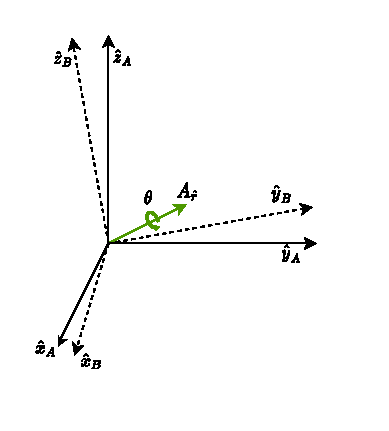
\includegraphics[width=0.7\textwidth]{figures/rotation.pdf}
  \caption{ 3D rotation around vector $\hat{r}$ between frame A and B. }
  \label{fig:rotation}
\end{figure}

\begin{equation}
  \begin{bmatrix}
    \dot{\psi}   \\
    \dot{\theta} \\
    \dot{\phi}   \\
  \end{bmatrix}
  =
  \frac{1}{\cos(\theta)}
  \begin{bmatrix}
    \sin(\phi)             & 0 & -\cos(\phi)            \\
    \cos(\theta)\cos(\phi) & 0 & \cos(\theta)\sin(\phi) \\
    \sin(\theta)\sin(\phi) & 1 & \sin(\theta)\cos(\phi)
  \end{bmatrix}
  \begin{bmatrix}
    \omega{^b_{nbx}} \\
    \omega{^b_{nby}} \\
    \omega{^b_{nbz}} \\
  \end{bmatrix}
  \label{eq:euler_equation}
\end{equation}

\begin{equation}
  {^b_a}R = {^b_2}R_x(\phi){^2_1}R_y(\theta){^1_a}R_z(\psi)
  =
  \begin{bmatrix}
    \sin(\phi)             & 0 & -\cos(\phi)            \\
    \cos(\theta)\cos(\phi) & 0 & \cos(\theta)\sin(\phi) \\
    \sin(\theta)\sin(\phi) & 1 & \sin(\theta)\cos(\phi)
  \end{bmatrix}
  \label{eq:euler_equations}
\end{equation}

Nevertheless, there is a significant flaw with this approach. As cos($\theta$) approaches zero, the differential equations degrade rapidly and the output solution becomes vastly imprecise, which indicates that these equations cannot provide effective attitude results at unique points in space \cite{spring1986euler}. This is also known as Gimbal lock. Euler angles can be represented as a gimballed system, where the three axes can be thought of as three distinct gimbals attached together \cite{mcconnell1967kinematics}. Gimbal lock happens when two axes line up, such as when the pitch and the yaw axis are aligned, and as the roll gimbal is rotated, the pitch and the yaw angle are both affected simultaneously, consequently losing orientation (figure \ref{fig:gimbal_lock}) \cite{hemingway2018perspectives}.
Euler angles commonly involve a large number of complex mathematical operations, such as matrix manipulations, which typically take up several clock cycles in a CPU, such can negatively impact computational performance. In this dissertation, a different kind of orientation representation will be used quaternions.

\begin{figure}[!h]
  \centering
  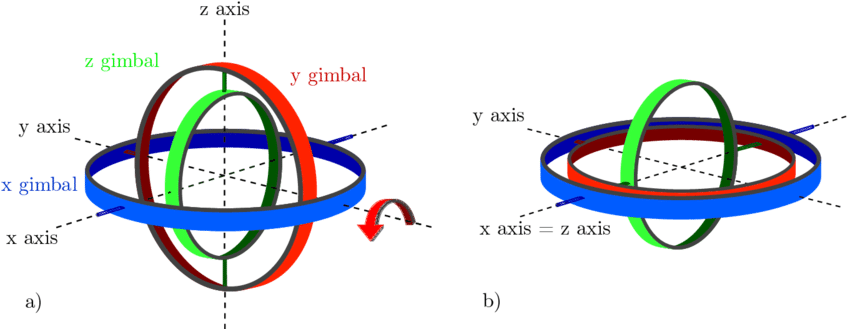
\includegraphics[width=0.7\textwidth]{figures/gimbal_lock.png}
  \caption{Representation of the Gimbal Lock problematic \cite{zeitlhofler2019nominal} - The exterior blue gimbal characterizes the x-axis, the middle, red-colored gimbal the y axis, and the inner green gimbal the z-axis. In the initial arrangement a), every axis is perpendicular to one another. Following a rotation of 90º across the red arrow (y-axis), the blue and the green gimbals occupy the same rotation axis. This condition inhibits the clear determination of the rotation axes when subsequently rotating around the x or z-axis. }
  \label{fig:gimbal_lock}
\end{figure}

\subsubsection{Quaternions}

Another commonly used attitude representation is the quaternion. To comprehend quaternions, one must first grasp the complex number relationship. A complex number can depict a rotation in a 2-dimensional coordinate frame with a real x-axis and an imaginary y-axis (or vice versa) (figure \ref{fig:complex_rotation}) \cite{lee2008representing}. A quaternion builds upon this concept, but rather than one imaginary axis, it makes use of three imaginary axes: similar to merging three complex numbers into one. Four components are required to progress from a two-dimensional definition to a three-dimensional plane: one real component $q_0$ and three imaginary $q_1$, $q_2$ and $q_3$. Quaternions are mathematically denoted as equation \ref{eq:quaternion_representation}, and are commonly represented as a vector (equation \ref{eq:quaternion_vector}), where $q_0$ is the norm, $q_1$, $q_2$, and $q_3$ are complex coordinates with $i$, $j$, $k$ being the axis versors. Equation (2.1) shows this relation with the complex number x having a real part a and imaginary part b; and the quaternion q containing a real scalar part s and an imaginary vector component ~v \cite{mukundan2002quaternions}.

\begin{figure}[!h]
  \centering
  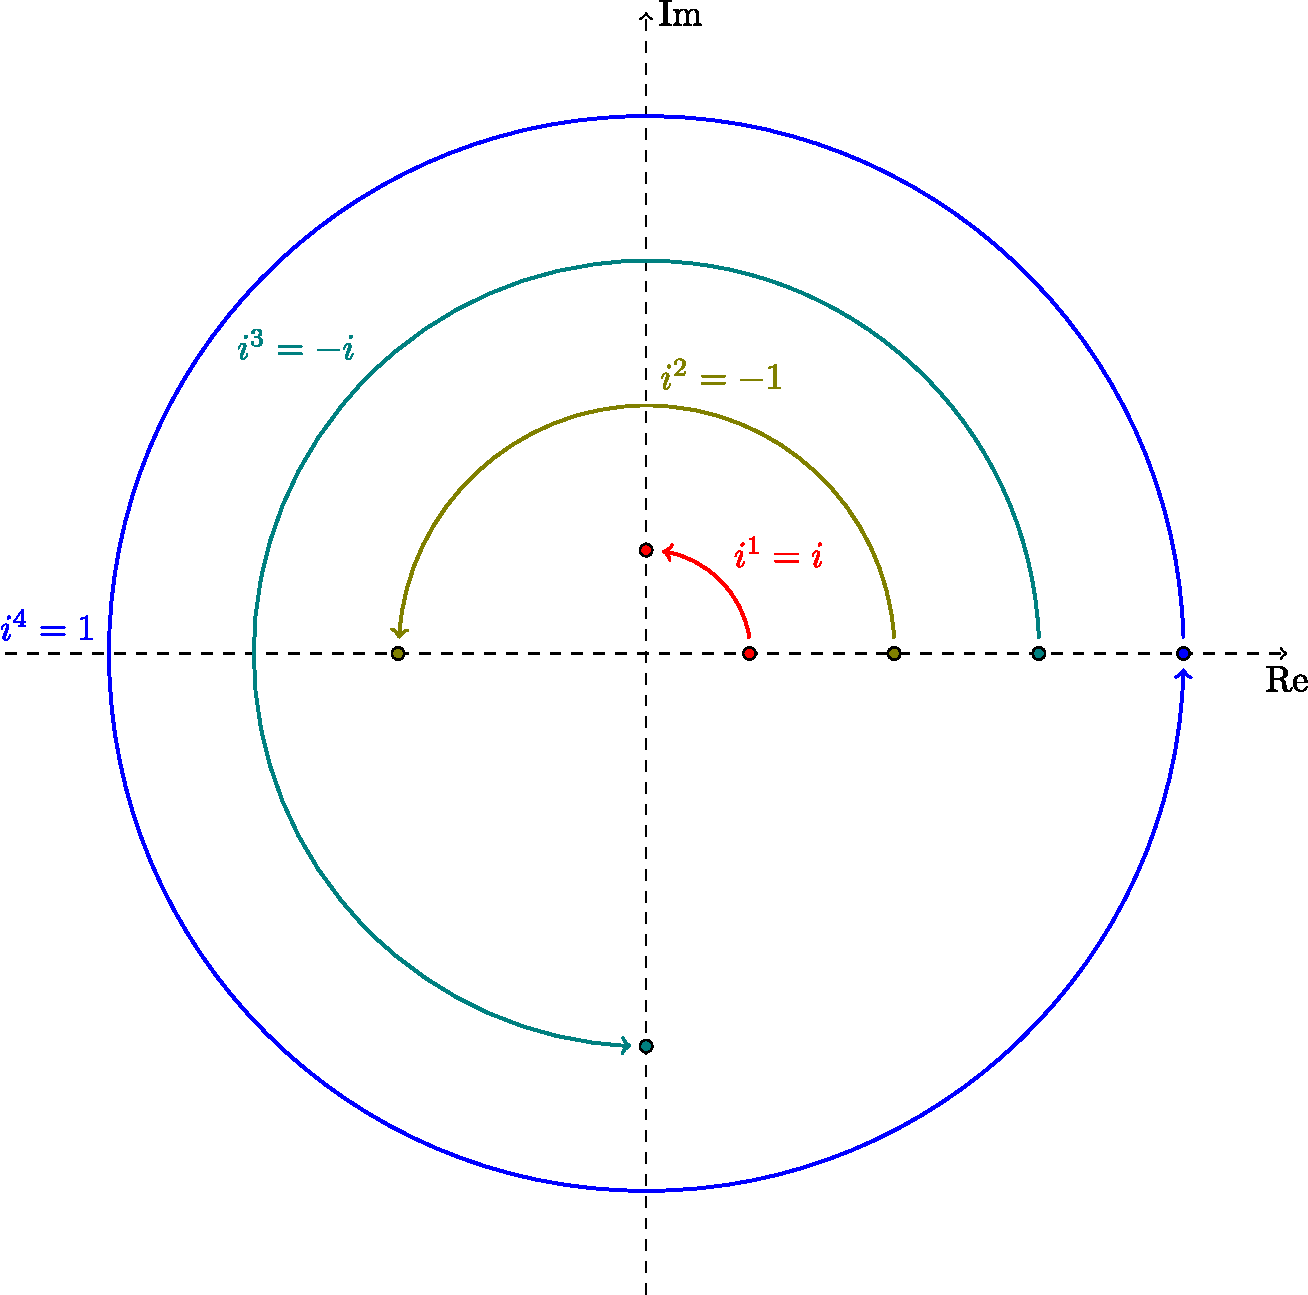
\includegraphics[width=0.7\textwidth]{figures/complex_rotation.pdf}
  \caption{90-degree rotation in a 2-dimensional coordinate frame with a real x-axis and an imaginary y-axis. }
  \label{fig:complex_rotation}
\end{figure}

\begin{equation}
  q = q_0 + q_1 i + q_2 j + q_3 k
  \label{eq:quaternion_representation}
\end{equation}

\begin{equation}
  q =     \begin{bmatrix}
    q_0 & q_1 & q_2 & q_3 \\
  \end{bmatrix}
  \label{eq:quaternion_vector}
\end{equation}

Specifically, when used for attitude description the quaternions should have a norm equal to 1 \cite{valenti2015keeping}:

\begin{equation}
  \left\lVert q\right\rVert =\sqrt{q^2_0 + q^2_1 + q^2_2 + q^2_3} =1
\end{equation}

Normalizing a quaternion is identical to normalizing a vector \cite{bar1985attitude}. The quaternion $q$ is divided by the norm of the quaternion $\left\lVert q \right\rVert$. When a quaternion is normalized, it is known as unit quaternion (also mentioned as versor of $q$) and denoted with a circumflex accent ($\hat{q}$):

\begin{equation}
  \hat{q} = \frac{q}{\left\lVert q \right\rVert }
\end{equation}


A quaternion's conjugate ($q^{\ast} $) is expressed by:

\begin{equation}
  q^{\ast}  =\begin{bmatrix}
    q_0 & -q_1 & -q_2 & -q_3 \\
  \end{bmatrix}
\end{equation}

The inverse of a quaternion (${q^{-1}}$) is therefore given by:

\begin{equation}
  q^{-1} = \frac{q^{\ast} }{\left\lVert q \right\rVert }
\end{equation}

Applying the notation as declared previously, ${^w_b}q$ constitutes the orientation of body frame ($b$) with respect to world frame ($w$). From equation \ref{eq:quaternion_representation}, the subsequent list of properties/operations is derived:

\item \textbf{Multiplication of basis elements} Every quaternion multiplication of basis elements $\boldsymbol{i}$, $\boldsymbol{j}$ and $\boldsymbol{k}$ ought to follow the succeeding list of properties (also visible in table \ref{tab:quaternion_multiplication} containing multiplication of basis elements):


\begin{equation}
  \begin{gathered}
    i^2=j^2=k^2=ijk=-1 \\
    ij = -ji = k       \\
    jk = -kj = i       \\
    ki = -ik = j       \\
  \end{gathered}
  \label{eq:quaternion_rules}
\end{equation}

\begin{figure}[H]
  \centering
  \begin{table}[H]
    \begin{center}
        \begin{tabular}[t]{l|cccc}
            \hline
            $\times$ & $1$ & $i$  & $j$  & $k$  \\
            \hline
            $1$      & $1$ & $i$  & $j$  & $k$  \\
            $i$      & $i$ & $-1$ & $k$  & $-j$ \\
            $j$      & $j$ & $-k$ & $-1$ & $i$  \\
            $k$      & $k$ & $j$  & $-i$ & $-1$ \\
            \hline
        \end{tabular}
        \caption{Quaternion multiplication of basis elements. }
        \label{tab:quaternion_multiplication}
    \end{center}
\end{table}
\end{figure}

\item \textbf{Multiplication of quaternions} The product of two quaternions, $a$ and $b$, is denoted by $\otimes$ and it is defined by the Hamilton product. It can be calculated by the product of the basis elements and the distributive law. The product can then be expanded by the distributive law into a a sum of products of basis elements. Returning the next expression:

\begin{equation}
  a \otimes b = \left[a_0 a_1 a_2 a_3\right] \otimes \left[b_0 b_1 b_2 b_3\right]     =
  \begin{bmatrix}
    a_0 b_0 + a_1 b_0\boldsymbol{i} + a_2 b_0\boldsymbol{j} + a_3 b_0\boldsymbol{k}                   \\
    a_0 b_1\boldsymbol{i} + a_1 b_1\boldsymbol{i^2} + a_2 b_1\boldsymbol{ij} + a_3 b_1\boldsymbol{ik} \\
    a_0 b_2\boldsymbol{j}+ a_1 b_2\boldsymbol{ji} + a_2 b_2\boldsymbol{j^2} + a_3 b_2\boldsymbol{jk}  \\
    a_0 b_3\boldsymbol{k} + a_1 b_3\boldsymbol{ki} + a_2 b_3\boldsymbol{kj} + a_3 b_3\boldsymbol{k^2} \\
  \end{bmatrix}
\end{equation}

As a result, the rules defined in equation \ref{eq:quaternion_rules} and table \ref{tab:quaternion_multiplication} can be applied at this step producing:

\begin{equation}
  a \otimes b =
  \begin{bmatrix}
    a_0 b_0 - a_1 b_1 - a_2 b_2 - a_3 b_3                 \\
    (a_0 b_1 + a_1 b_0 + a_2 b_3 - a_3 b_2)\boldsymbol{i} \\
    (a_0 b_2 - a_1 b_3 + a_2 b_0 + a_3 b_1)\boldsymbol{j} \\
    (a_0 b_3 + a_1 b_2 - a_2 b_1 + a_3 b_0)\boldsymbol{k} \\
  \end{bmatrix}
  \label{eq:quaternion_matrix}
\end{equation}

\item \textbf{Quaternion conjugate} Conjugation is an involution (a function that is its own inverse), conjugating an element twice yields the original constituent. The conjugate of a quaternion relates to an inverse rotation, in this case constitutes the orientation of world frame with respect to body frame:

\begin{equation}
  \textrm{$_{b}^{w}q$}^* =\textrm{$_{w}^{b}q$} = \left[q_1 - q_2 - q_3 - q_4\right]
\end{equation}

\item \textbf{Vector rotation} Let's define the following quaternion representation of the same vector but in each referential by using is pure quaternion as

$ ^wv = \begin{bmatrix}
    0 & ^wx & ^wy & ^wz
  \end{bmatrix} $
and
$^bv = \begin{bmatrix}
    0 & ^bx & ^by & ^bz
  \end{bmatrix} $. The rotation of vector $v$ from one frame to other, using a quaternion, is performed by equation 2.10.

\begin{equation}
  \textrm{$^{b}v$} = \textrm{$_{b}^{w}\hat{q}$} \otimes \textrm{$^{w}v$} \otimes \textrm{$_{b}^{w}\hat{q}$}^*
\end{equation}

\item \textbf{Composed rotations} The composition of rotations can be described in quaternions as the product between quaternions. For example, the sequence a $^a_b\hat{q} \rightarrow {^b_c\hat{q}}$ is equal to $^a_c{\hat{q}}$ and is defined as equation 2.11.


\begin{equation}
  \textrm{$_{c}^{a}\hat{q}$} = \textrm{$_{c}^{b}\hat{q}$} \otimes \textrm{$_{b}^{a}\hat{q}$}
\end{equation}

\subsection{Inertial Measurement Units}

An inertial measurement unit (IMU) is an electronic tool that quantifies and describes specific force, angular rate, and occasionally the orientation of a body. It comprises an amalgamation of accelerometers, gyroscopes, and optionally magnetometers. They have also become standard in embedded inertial systems due to their low cost, lightweight, and low power consumption. IMUs are normally employed in aircraft maneuvering (via an attitude and heading reference system), such as spacecrafts \cite{li2011calibration} \cite{haberberger2016imu} \cite{faragher2012understanding}, satellites \cite{lu2020orbit}, and unmanned aerial vehicles (UAVs) \cite{sahawneh2008development} \cite{eling2015real}, to name a few. IMUs have been employed in wearable applications with uses in  telemedicine \cite{madgwick2020extended} \cite{allen2013telemedicine} \cite{giansanti2009toward} \cite{o2021measuring}, and robotics \cite{wilson2019formulation}. Newly developed IMUs integrate satellite localization capabilities permitting these devices to operate even when satellites signals are unobtainable, such as in tunnels, indoors, or in the presence of electronic interference.
There are several different types of sensor errors. These can be noise, offset, drift, scale factor error, non-linearity, and accuracy error \cite{hanke2016classification}. The main errors that cause unreliable readings are high frequent noise, offset error and drift error. Thus, these three will be considered and reduced using suitable filters.

\begin{figure}[!h]
  \centering
  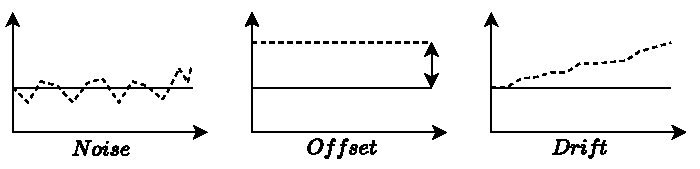
\includegraphics[width=1\textwidth]{figures/noise.pdf}
  \caption{Three main types of sensor error}
  \label{fig:noise}
\end{figure}

The first graph in the picture above represents the signal error classified as noise. The noise is high frequent and can be eliminated by using a low pass filter \cite{kaiser1977data}. The noise sources in the sensor can be categorized into three types.
1. Environmental noise, such as temperature fluctuations, gravity , etc.
2. Movements, such as vibrations, shocks .
3. Hardware noise, such as electrical and mechanical thermal noise.

The second graph is the offset error, called bias error. This error results in a shift from the zero value and can be solved by subtracting the DC component with a high pass filter. In the last graph the drift error is presented. The drift components occur from vibration, shock, and temperature variations. The main drift component in this study will be caused by numerical integration during the position calculation.
Temperature changes may cause fluctuations in the bias of the sensor signal. By using an additional sensor to measure the ambient temperature the bias induced error can be compensated by applying corrections to the output signals. The relationship between bias error and temperature depends on the sensor device. For a gyroscope the temperature change will cause an error in orientation which grows linearly with time. For an accelerometer the temperature will cause an error in position, thus grow quadratically with time. For the magnetometer the increasing temperature will lead to softening in the moving structure.

\subsubsection{Accelerometer}

An accelerometer is a device capable of measuring proper acceleration. Proper acceleration is the physical acceleration experienced by an object. It is thus acceleration relative to an inertial observer who is momentarily at rest relative to the object being measured \cite{pons2019observers}. As an example, if an accelerometer would be placed at rest on the surface of the Earth, it will measure an upwards acceleration due to Earth's gravity of g $\simeq$ 9.81 $m/s^2$. This is due to the Earth's surface exerting a normal force upwards relative to the local inertial frame. On the other hand, a free-falling accelerometer (moving in the center of the Earth's direction at around 9.81 $m/s^2$) would quantify no acceleration. Acceleration is quantified in the SI unit meters per second ($m/s^2$), or standard gravity, denoted by $g_n$, being the nominal gravitational acceleration of an object in a vacuum near the surface of the Earth. It is defined by standard as 9.80665 $m/s^2$.

The working principle of an accelerometer can be expounded by a single mass ($m$) fixed to a stiffness spring ($k$) that in turn is fastened to outer frame, as illustrated in figure \ref{fig:accelerometer_schematic} \cite{roylance1979batch}.

\begin{figure}[!h]
  \centering
  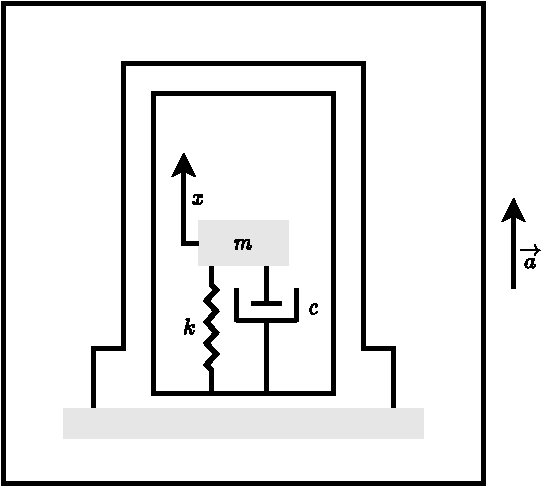
\includegraphics[width=0.5\textwidth]{figures/accelerometer.pdf}
  \caption{Schematic demonstrating the working principle of an accelerometer. \cite{roylance1979batch} }
  \label{fig:accelerometer_schematic}
\end{figure}

Often, the structure incorporates a dashpot (mechanical device which resists motion via viscous friction). The dashpot has a resistive coefficient ($c$) and is tied to the mass parallelly to the spring. When the system is affected by a linear acceleration, a force equivalent to mass times the acceleration acts upon the mass, causing it to deflect. This deflection is then converted into an analogous electrical signal. The dashpot mechanism causes the system to quickly stabilize following the acceleration. To derive the motion equation of the system Newton's second law is used, where all real forces acting on the proof-mass are equal to the inertia force on the mass. With $x$ being the displacement of the mass $m$ relative to the outer system. When the system is subject to an acceleration a, the equation of motion for the mass is:

\begin{equation}
  mx + kx + cx = \overrightarrow{F}\Leftrightarrow mx + kx + cx = m\overrightarrow{a}
\end{equation}

Where $c$ and $k$ are the dashpot resistive coefficient and spring stiffness constant, respectively. Consequently, the acceleration can be computed by measuring $x$, compression of the spring.


\subsubsection{Gyroscope}

A gyroscope is a device utilized to quantify angular velocity and orientation based on the principles of conservation of angular  \cite{zhuang2020introductory}. A conventional gyroscope accommodates a spinning wheel mounted on two gimbals letting it spin in all three axes, as shown in figure \ref{fig:gyroscope}. The rotating wheel will resist changes in orientation as an effect of the angular momentum. As a result, when a rotation is exerted on the mechanical gyroscope, the wheel will persist in its global orientation meanwhile the angles between neighboring gimbals will change \cite{marotto2013orientation}.

\begin{figure}[!h]
  \centering
  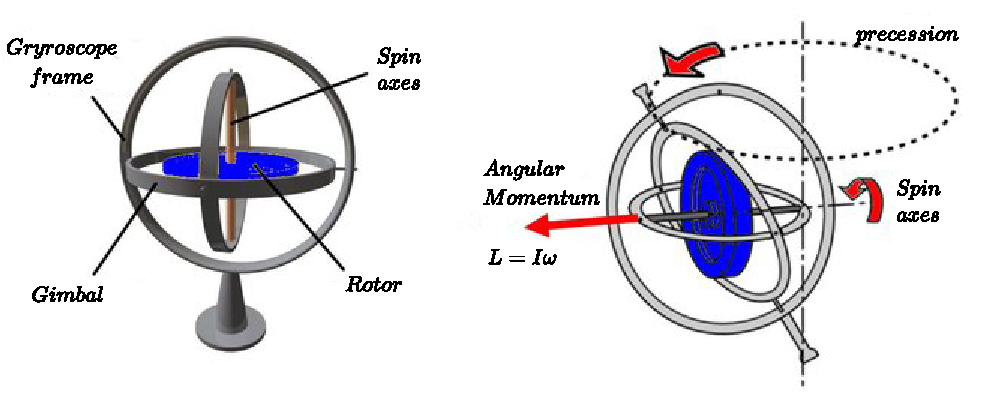
\includegraphics[width=0.7\textwidth]{figures/gyroscope.pdf}
  \caption{ Representation of a conventional gyroscope accommodating a spinning wheel mounted on two gimbals. \cite{marotto2013orientation} }
  \label{fig:gyroscope}
\end{figure}

A traditional mechanical gyroscope can merely evaluate orientation and since they contain moving parts, they can cause the output to drift over time. Modern gyroscopes (such as optical and MEMS gyroscopes) are rate-gyros, meaning they can detect angular velocity \cite{antonello2011mems}. Angular velocity ($\omega$) is quantified in the SI unit radians per second ($rad/s$), or degrees per second ($^{\circ}/s$). MEMS sensors constructed using silicon electrical methods have a smaller number of parts and are inexpensive to produce \cite{antonello2012exploring}. MEMS gyroscopes based on the Coriolis effect, which states that in a frame of reference rotating at angular velocity ($\omega$), a mass ($m$) moving with linear velocity ($v$) experiences a force (figure \ref{fig:coriolis}) \cite{trusov2011overview}:

\begin{equation}
  \overrightarrow{F}_{Coriolis} = -2m(\omega \times \overrightarrow{v} )
\end{equation}

Above, the cross product between angular velocity ($\omega$) and linear velocity ($v$) multiplies solely by orthogonal vector components. The outcome of the cross product is orthogonal to both $v$ and $\omega$. Its direction can be ascertained by the right-hand rule.

\begin{figure}[!h]
  \centering
  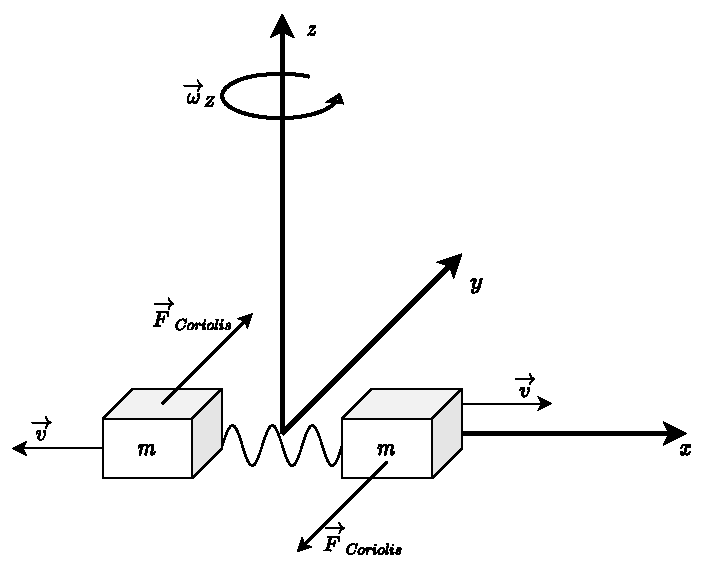
\includegraphics[width=0.7\textwidth]{figures/coriolis.pdf}
  \caption{ System where two masses are oscillating in opposite directions. When a rotation is applied, the masses are affected by the Coriolis force and the displacement is measured by a change in capacitance. \cite{passaro2017gyroscope}}
  \label{fig:coriolis}
\end{figure}

The gyroscope sensor measurements supply a body's angular rate, a measurement of the change in angle over time which is represented by $\omega(x)$ \cite{trusov2011overview}:

\begin{equation}
  \omega(x) = \frac{dx}{dt}
\end{equation}

The angular rate supplied by the gyroscope sensor can be integrated over an interval of time ($t$) and a sampling period ($T_s$). The sum of every measurement will return an absolute angle $\theta$. The integration of the angular rate is shown in equation $\ref{eq:angular_integration}$ \cite{trusov2011overview}:

\begin{equation}
  \theta = \int_{0}^{t} \omega(x) dx = \sum_{0}^{t} \omega(x)\cdot T_s
  \label{eq:angular_integration}
\end{equation}

Given a set of angular rates $w=[w_x,w_y,w_z]$ measured by the gyroscope, by equation \ref{eq:quaternion_matrix} it is possible to convert the set into a matrix of quaternion rates ($\Omega$) \cite{trusov2011overview}:

\begin{equation}
  \Omega = \begin{bmatrix}
    0   & -w_x & -w_y & -w_z \\
    w_x & 0    & w_z  & -w_y \\
    w_y & -w_z & 0    & w_x  \\
    w_z & w_y  & -w_x & 0    \\
  \end{bmatrix}
\end{equation}

From a quaternion rate at instant $t-1$, given a current angular speed it is possible to estimate the quaternion at instant $t$. Quaternion $q_t$ revolved by the gyroscope, the antecedent attitude quaternion $q_{t-1}$ is multiplied by $\Omega$, then half of the period $Ts$ \cite{trusov2011overview}.

\begin{equation}
  q_t = q_{t-1} \ast \Omega \ast \frac{1}{2} \ast T_s
\end{equation}

\subsubsection{Magnetometer}

A magnetometer is an electronic utensil that evaluates existent magnetic flux (a magnetic field's intensity). Magnetic flux is quantified in the SI unit microtesla ($\mu T$). Certain magnetometers can detect the orientation, magnitude, or relative change of a magnetic field \cite{caruso1998new}. A magnetometer accompanied with an accelerometer can successfully reckon an orientation angle. The magnetometer readings uniquely are not able to perceive a heading angle due to the presence of all sorts of distortions such as of the earth's own magnetic fields or even local disturbances of nearby metallic bodies on the sensor \cite{silva2021error} \cite{caruso1998new}. There are two categories of magnetic distortions: Hard iron and soft iron \cite{wahdan2014magnetometer}. Hard iron distortions are generated by materials that exhibit a continuous additive field, and as a result produce a persistent additive value to the measurements of the magnetometer \cite{guo2008soft}. A piece of magnetized iron or a speaker, for example, will induce a hard iron distortion in the magnetometer. If the orientation and position of the magnetic disturbance relative to the sensor is unchanging, the magnetic offset will remain constant. It is possible to compensate for hard-iron disturbances by discerning the maximum and minimum x and y offsets. The x axis and y axis offset ($\alpha$ and $\beta$, respectively) are given by the average of the maximum ($x_{max}$ and $y_{max}$) and minimum ($x_{min}$ and $y_{min}$) values for each axis \cite{daponte2017method}:

\begin{equation}
  \begin{gathered}
    \alpha = \frac{x_{max}+x_{min}}{2}\\
    \beta = \frac{y_{max}+y_{min}}{2}
  \end{gathered}
\end{equation}

By subtracting these offsets from the magnetometer readings, it is possible to substantially remove any present hard-iron disturbances.

Soft-iron distortion is the consequence of a material's influence that can warp a magnetic field but does not necessarily produce a magnetic field itself, and as a result is not additive \cite{bachmann2004investigation}. Unlike hard-iron distortion which has a continuous disturbance, a soft-iron distortion is determined by the direction of the material in respect to the sensor and the magnetic field of the same material. Calculating the soft iron distortion is computationally more expensive than the hard iron elimination. There are two axes to consider, the major and the minor axes \cite{roetenberg2005compensation}.

The major axis is the axis that runs along the x axes. This will be used to find the angle $\theta$ by calculating the magnitude of the line segment. Essentially by computing r, it is the same as calculating the magnitude of each point on the ellipse and finding the maximum point \cite{daponte2017method}.

\begin{equation}
  r=\sqrt{(x_1)^2+(y_1)^2}
\end{equation}

\begin{equation}
  \theta=\arcsin(\frac{y_1}{r})
\end{equation}

\begin{figure}[!h]
  \centering
  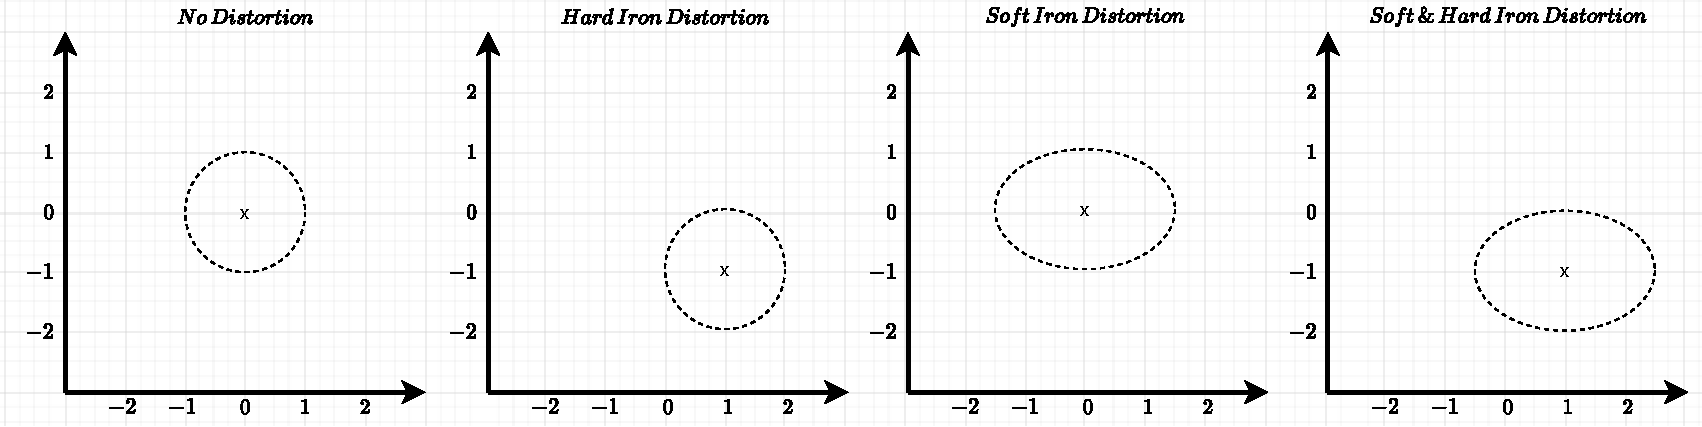
\includegraphics[width=1\textwidth]{figures/magnetometer_distortion.pdf}
  \caption{Representation of a magnetometer's different types of disturbances. \cite{daponte2017method} }
  \label{fig:magnetometer_distortion}
\end{figure}



\subsection{Sensor Fusion}
\label{sub:sensor_fusion}

Sensor fusion defines the blending of sensory information from two or more sources in a way that generates a more consistent and dependable understanding of the system. One that would otherwise not be possible when these sources were used individually \cite{bostrom2007definition}. Ideally, a gyroscope could deduce a body's attitude independently. As mentioned previously, integrating the gyroscope's readings can ascertain the attitude solution of a body. Notwithstanding, with less cost comes lower accuracy and precision. This originates from a drift build up on the gyro's readings, where error accumulates exponentially on the integrated output \cite{borenstein2009heuristic}. The accelerometer and magnetometer can work together to evaluate attitude straight from measurements of acceleration and present magnetic fields. This combination is often corrupted by disturbances such as vibrations and local magnetic interferences \cite{silva2021error}. Hence, both solutions have their respective benefits and require a rectifying term from an additional sensor. This conducts to a demand for a sensor fusion algorithm that combines both solutions in a way that emphasizes their strengths and minimizes their weaknesses \cite{hol2011sensor}. A sensor fusion algorithm will decide on the optimal trust combination of each sensor to assess attitude. A diversity of suitable algorithms exist that can fuse the output of different sensors to create a more reliable and consistent signal. This chapter will highlight some of the most prominent sensor fusion algorithms in existence:

\subsubsection{Kalman Filter}

The Kalman filter algorithm is a set of mathematical equations that provides a computationally efficient approach to estimate some unknown variables by the detected measurements\cite{welch1995introduction}. Kalman filters operate recursive functions to predict the present state of a linear problem by monitoring the current input data, the previous input data, and the previous state prediction. Two generally assigned methods for Kalman filter-based sensor fusion are state-vector fusion and measurement fusion. The state-vector fusion method (figure \ref{fig:state_kalman}) applies a group of Kalman filters to acquire individual sensor-based state estimates, which are subsequently fused to obtain an enhanced combined state estimate.

\begin{figure}[!h]
  \centering
  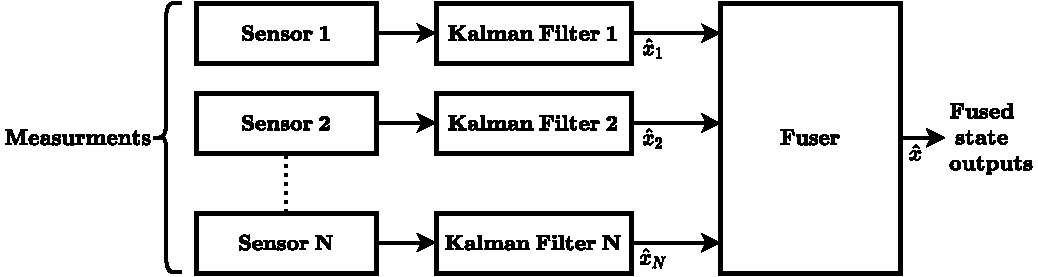
\includegraphics[width=0.7\textwidth]{figures/kalman1.pdf}
  \caption{Kalman-filter-based multi-sensor state-vector fusion. \cite{mosallaei2007process}}
  \label{fig:state_kalman}
\end{figure}

Measurement fusion (figure \ref{fig:mesearurment_kalman}) approach directly combines the sensor data to achieve a joint measurement and later uses a single Kalman filter to get hold of the final state estimate centered on the fused measurement \cite{mosallaei2007process}.

\begin{figure}[!h]
  \centering
  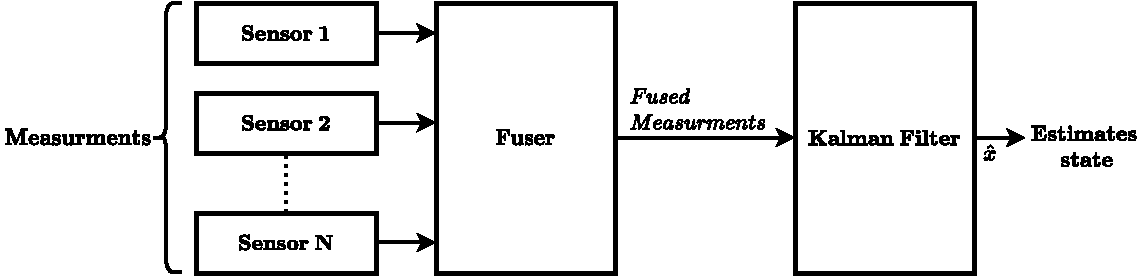
\includegraphics[width=0.7\textwidth]{figures/kalman2.pdf}
  \caption{Kalman-filter-based multi-sensor easurement fusion. \cite{mosallaei2007process}}
  \label{fig:mesearurment_kalman}
\end{figure}

When applied appropriately, Kalman filters offer highly precise orientation, even with the existence of substantial noise. Nevertheless, Kalman filters are computationally expensive rising hardware cost and latency. They are also of complex implementation, which, shared with computational overhead, can make the algorithm unfeasible for computationally restricted applications. They are regularly useful in a wide-ranging variety of applications and have become a standard method in sensor fusion. Several studies examine the possibility of using Kalman filters to predict a body's orientation and position by combining multiple sensors. The Kalman filter is founded on recursive Bayesian filtering.
Consequently, the system's noise is assumed to be Gaussian. Therefore, the Kalman filter is generally suggested for linear systems. For this reason, an extension of the classic Kalman Filter designed for non-linear systems has emerged, recognized as Extended Kalman filter \cite{wilson2019formulation}.

% \begin{figure}
%     \centering
%     \begin{subfigure}[b]{0.45\textwidth}
%         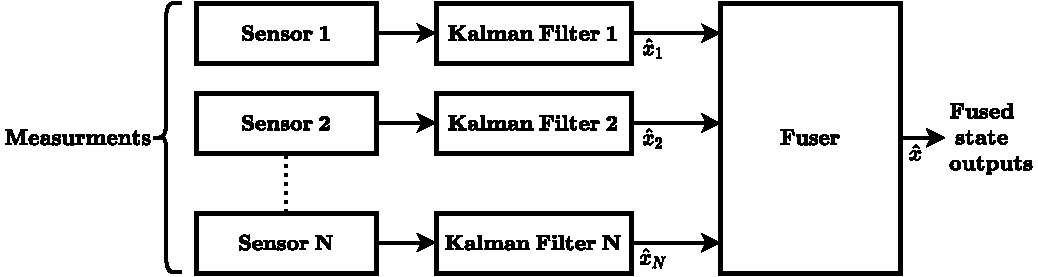
\includegraphics[width=1\linewidth]{figures/kalman1.pdf}
%         \caption{}
%         \label{fig:state_kalman}
%     \end{subfigure}
%     \begin{subfigure}[b]{0.45\textwidth}
%         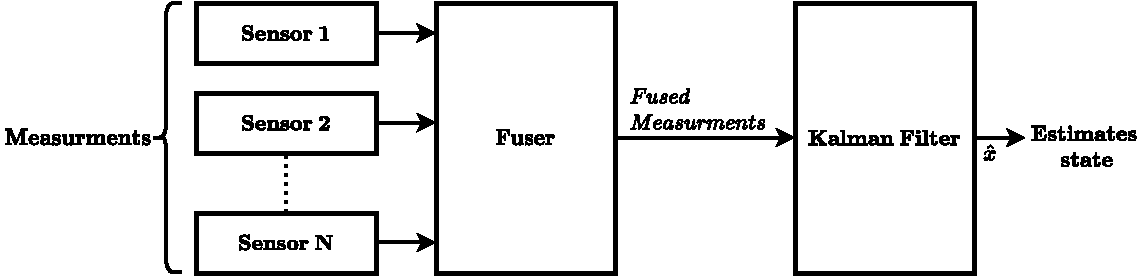
\includegraphics[width=1\linewidth]{figures/kalman2.pdf}
%         \caption{}
%         \label{fig:mesearurment_kalman}
%     \end{subfigure}

%     \caption{ Kalman-filter-based multi-sensor data fusion.
%         (a) State-vector fusion. (b) Measurement fusion. \cite{mosallaei2007process} }
% \end{figure}

\subsubsection{Complementary Filter}

The complementary filter is considered a simpler approach relatively to the Kalman filter since it is a computationally lightweight solution and straightforward to implement \cite{higgins1975comparison}. This filter takes as input two noisy sensor measurements and assumes one input is mainly formed by high-frequency signals whereas the other is mostly by low-frequency signals. Through a low pass filter, the high-frequency noise of the first input is filtered out. An identical procedure occurs with the second signal, but this time with a high pass filter to remove low-frequency noises, as illustrated in figure \ref{fig:complementary}.

\begin{figure}[!h]
  \centering
  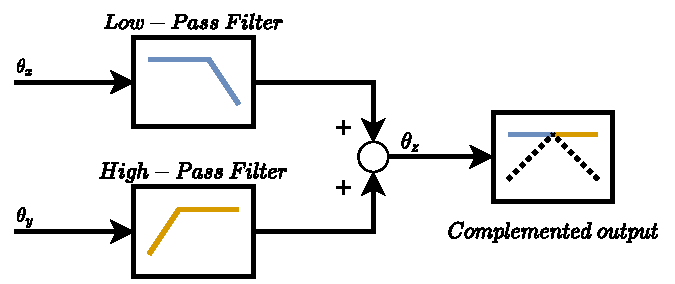
\includegraphics[width=0.7\textwidth]{figures/complementary.pdf}
  \caption{Basic complementary filter \cite{higgins1975comparison} - Two different measurement sources for estimating one variable. The noise properties of the two measurements are such that one source gives good information only in low frequency region while the other is good only in high frequency region. }
  \label{fig:complementary}
\end{figure}

The accelerometer is especially vulnerable to vibrations and centripetal forces, these can be filtered by a low pass filter behaving as a moving average filter. The gyroscope is precise and exact in the short term, but quickly loses precision in integration due to drift. For that reason, a high pass filter that allows the short-term gyroscope data is desirable, thus, removing the long-term drift.
At any given moment, the complete the signal is subject to a low pass filter (equation \ref{eq:low_pass_filter}) or a high pass filter (equation \ref{eq:high_pass_filter}), where $\theta_t$ represents current orientation, $\alpha$ is a filter coefficient, $\omega$ the gyro's angular velocity and $a$ the acceleration obtained from the accelerometer:

\begin{equation}
  y_t = (1-\alpha)x_{t} + \alpha y_{t-1}
  \label{eq:low_pass_filter}
\end{equation}

\begin{equation}
  y_t = (1-\alpha)y_{t-1} + (1-\alpha) (x_t - x_{t-1})
  \label{eq:high_pass_filter}
\end{equation}

$\alpha$ filter coefficient describes the borderline where the gyroscope measurements end, and the accelerometer readings begin and vice versa. It rules how much the output relies on the current reading or a new value that arrives. $\alpha$ is typically above 0.5 by the definition above. Where the filter coefficient $\alpha$ is determined by:

\begin{equation}
  \alpha = \frac{\tau}{\tau + \Delta t}
\end{equation}

Where $\tau$ is the wanted time constant (time interval for the readings to respond) and $\Delta t$ is the sampling period.

\begin{equation}
  \theta = \frac{\tau}{\tau + s}a + \frac{s}{\tau + s}\frac{1}{s}\omega = \frac{a+\tau \omega}{\tau + s}
\end{equation}

A mathematical model of the complementary filter can be represented as equation \ref{eq:complementary_model}, where $\theta_t$ represents current orientation, $\alpha$ is the filter coefficient, $\omega$ the gyro's angular velocity and $a$ the acceleration obtained from the accelerometer:

\begin{equation}
  \theta_t = (1 - \alpha) (\theta_{t-1} + \omega \Delta t) + \alpha a
  \label{eq:complementary_model}
\end{equation}

Yet, the complementary filter is not especially robust to noisy or biased data since it simply uses currently available information, therefore, has no direct method of compensating for sensor noise \cite{wilson2019formulation}. A conventional application of the complementary filter is to bring together measurements of vertical acceleration and barometric readings to attain an approximation of vertical velocity. Similar to the Kalman filter, new versions built upon the principles of the classic complementary filter have emerged in recent times, such as the Extended Complementary Filter (ECF). They promise a high level of accuracy and enhanced robustness to noise while preserving computational efficiency.

\subsubsection{Optimization Filters}

Up until recently, there remained mainly two distinct AHRS fusion approaches. One category including the complementary filters, and the other is related to Kalman filtering. Some recent AHRS algorithms have emerged in the literature over the past years. Two of the most prominent are the Mahony and Madgwick algorithms, which have been categorized as optimization filters. Optimization filters obtain orientation by assessing a vector representative of the sensor output at the present orientation and lessening the disparity concerning predicted and observed outputs. Optimization filters are well established for linking accuracy with computational expense and simplicity of implementation \cite{madgwick2020extended}.
Both methods make use of a quaternion representation, which is a four-dimensional complex number representing of an object orientation. Quaternions involve fewer computation time because of their minimal quantity of calculation parameters \cite{ludwig2018comparison}. Additionally, vector rotations are easily executed by quaternion multiplications.
Madgwick et al. \cite{madgwick2010efficient} pioneered a gradient descent fusion algorithm, frequently recognized as 'Madgwick Algorithm.' This gradient descent fusion algorithm first obtains a quaternion estimation of the gyroscope output integration and later corrects it with a quaternion from the accelerometer and magnetometer data. Madgwick's approach guarantees decent attitude estimation at a low computational cost. Further, it tackles the difficulty of the local magnetic disturbances that can influence all the orientation components. By reducing the constraint of the magnetic field vector rotation, it can limit the effect of the magnetic disturbances to only affect the yaw component of the orientation.

\paragraph{Other Filters}
% \subsection{Low-Cost Inertial Measurement Units}
% \subsubsection{MPU-9150 Evaluation Board 9DOF}
